
\documentclass[12pt,a4paper,doublesided,openright]{book}

\usepackage{mathbf-abbrevs}
%\usepackage{natbib}
\usepackage{pgfplots}
%\newcommand {\tbf}[1] {\textbf{#1}}
%\newcommand {\tit}[1] {\textit{#1}}
%\newcommand {\tmd}[1] {\textmd{#1}}
%\newcommand {\trm}[1] {\textrm{#1}}
%\newcommand {\tsc}[1] {\textsc{#1}}
%\newcommand {\tsf}[1] {\textsf{#1}}
%\newcommand {\tsl}[1] {\textsl{#1}}
%\newcommand {\ttt}[1] {\texttt{#1}}
%\newcommand {\tup}[1] {\textup{#1}}
%
%\newcommand {\mbf}[1] {\mathbf{#1}}
%\newcommand {\mmd}[1] {\mathmd{#1}}
%\newcommand {\mrm}[1] {\mathrm{#1}}
%\newcommand {\msc}[1] {\mathsc{#1}}
%\newcommand {\msf}[1] {\mathsf{#1}}
%\newcommand {\msl}[1] {\mathsl{#1}}
%\newcommand {\mtt}[1] {\mathtt{#1}}
%\newcommand {\mup}[1] {\mathup{#1}}

%some math functions and symbols
\newcommand{\reals}{{\mathbb R}}
\newcommand{\ints}{{\mathbb Z}}
\newcommand{\complex}{{\mathbb C}}
\newcommand{\integers}{{\mathbb Z}}
\newcommand{\sign}[1]{\operatorname{sgn}\left( #1 \right)}
\newcommand{\NP}{\operatorname{NPt}}
\newcommand{\NS}{\operatorname{NearestSet}}
\newcommand{\bres}{\operatorname{Bres}}
\newcommand{\vol}{\operatorname{vol}}
\newcommand{\vor}{\operatorname{Vor}}
\newcommand{\coef}{\operatorname{coef}}
\newcommand{\eval}{\operatorname{eval}}
\newcommand{\from}{\colon}

\newcommand{\term}{\emph}
\newcommand{\var}{\operatorname{var}}
\newcommand{\covar}{\operatorname{covar}}
%\newcommand{\prob}{{\mathbb P}}
\newcommand{\prob}{\operatorname{Pr}}
\newcommand{\expect}{{\mathbb E}}
\newcommand{\dealias}{\operatorname{dealias}}
\renewcommand{\mid}{\; ; \;}

%distribution fucntions
\newcommand{\projnorm}{\operatorname{ProjectedNormal}}
\newcommand{\vonmises}{\operatorname{VonMises}}
\newcommand{\wrapnorm}{\operatorname{WrappedNormal}}
\newcommand{\wrapunif}{\operatorname{WrappedUniform}}

\newcommand{\selectindicies}{\operatorname{selectindices}}
\newcommand{\sortindicies}{\operatorname{sortindices}}
\newcommand{\largest}{\operatorname{largest}}
\newcommand{\quickpartition}{\operatorname{quickpartition}}
\newcommand{\quickpartitiontwo}{\operatorname{quickpartition2}}

%some commonly used underlined and
%hated symbols
\newcommand{\uY}{\ushort{\mbf{Y}}}
\newcommand{\ueY}{\ushort{Y}}
\newcommand{\uy}{\ushort{\mbf{y}}}
\newcommand{\uey}{\ushort{y}}
\newcommand{\ux}{\ushort{\mbf{x}}}
\newcommand{\uex}{\ushort{x}}
\newcommand{\uhx}{\ushort{\mbf{\hat{x}}}}
\newcommand{\uehx}{\ushort{\hat{x}}}

% Brackets
\newcommand{\br}[1]{{\left( #1 \right)}}
\newcommand{\sqbr}[1]{{\left[ #1 \right]}}
\newcommand{\cubr}[1]{{\left\{ #1 \right\}}}
\newcommand{\scubr}[1]{{\{ #1 \}}}
\newcommand{\abr}[1]{\left< #1 \right>}
\newcommand{\abs}[1]{\left\vert #1 \right\vert}
\newcommand{\sabs}[1]{\vert #1 \vert}
\newcommand{\floor}[1]{{\left\lfloor #1 \right\rfloor}}
\newcommand{\sfloor}[1]{{\lfloor #1 \rfloor}}
\newcommand{\ceiling}[1]{{\left\lceil #1 \right\rceil}}
\newcommand{\ceil}[1]{\lceil #1 \rceil}
\newcommand{\round}[1]{{\left\lceil #1 \right\rfloor}}
\newcommand{\sround}[1]{\lceil #1 \rfloor}
\newcommand{\magn}[1]{\left\| #1 \right\|}
\newcommand{\fracpart}[1]{\left\langle #1 \right\rangle}
\newcommand{\sfracpart}[1]{\langle #1 \rangle}

% Referencing
\newcommand{\refeqn}[1]{\eqref{#1}}
\newcommand{\reffig}[1]{Figure~\ref{#1}}
\newcommand{\reftable}[1]{Table~\ref{#1}}
\newcommand{\refsec}[1]{Section~\ref{#1}}
\newcommand{\refappendix}[1]{Appendix~\ref{#1}}
\newcommand{\refchapter}[1]{Chapter~\ref{#1}}

\newcommand {\figwidth} {100mm}
\newcommand {\Ref}[1] {Reference~\cite{#1}}
\newcommand {\Sec}[1] {Section~\ref{#1}}
\newcommand {\App}[1] {Appendix~\ref{#1}}
\newcommand {\Chap}[1] {Chapter~\ref{#1}}
\newcommand {\Lem}[1] {Lemma~\ref{#1}}
\newcommand {\Thm}[1] {Theorem~\ref{#1}}
\newcommand {\Cor}[1] {Corollary~\ref{#1}}
\newcommand {\Alg}[1] {Algorithm~\ref{#1}}
\newcommand {\etal} {\emph{~et~al.}}
\newcommand {\bul} {$\bullet$ }   % bullet
\newcommand {\fig}[1] {Figure~\ref{#1}}   % references Figure x
\newcommand {\imp} {$\Rightarrow$}   % implication symbol (default)
\newcommand {\impt} {$\Rightarrow$}   % implication symbol (text mode)
\newcommand {\impm} {\Rightarrow}   % implication symbol (math mode)
\newcommand {\vect}[1] {\mathbf{#1}} 
\newcommand {\hvect}[1] {\hat{\mathbf{#1}}}
\newcommand {\del} {\partial}
\newcommand {\eqn}[1] {Equation~(\ref{#1})} 
\newcommand {\tab}[1] {Table~\ref{#1}} % references Table x
\newcommand {\half} {\frac{1}{2}} 
\newcommand {\ten}[1] {\times10^{#1}}
\newcommand {\bra}[2] {\mbox{}_{#2}\langle #1 |}
\newcommand {\ket}[2] {| #1 \rangle_{#2}}
\newcommand {\Bra}[2] {\mbox{}_{#2}\left.\left\langle #1 \right.\right|}
\newcommand {\Ket}[2] {\left.\left| #1 \right.\right\rangle_{#2}}
\newcommand {\im} {\mathrm{Im}}
\newcommand {\re} {\mathrm{Re}}
\newcommand {\braket}[4] {\mbox{}_{#3}\langle #1 | #2 \rangle_{#4}} 
\newcommand{\dotprod}[2]{ #1^\prime #2}
\newcommand {\trace}[1] {\text{tr}\left(#1\right)}

% spell things correctly
\newenvironment{centre}{\begin{center}}{\end{center}}
\newenvironment{itemise}{\begin{itemize}}{\end{itemize}}

%%%%% set up the bibliography style
\bibliographystyle{IEEEbib}
%\bibliographystyle{uqthesis}  % uqthesis bibliography style file, made
			      % with makebst

%%%%% optional packages
\usepackage[square,comma,numbers,sort&compress]{natbib}
		% this is the natural sciences bibliography citation
		% style package.  The options here give citations in
		% the text as numbers in square brackets, separated by
		% commas, citations sorted and consecutive citations
		% compressed 
		% output example: [1,4,12-15]

%\usepackage{cite}		
			
\usepackage{siunitx}
	%nice looking units
		
\usepackage{booktabs}
		%creates nice looking tables
		
\usepackage{amsmath,amsfonts,amssymb, amsthm, bm} % this is handy for mathematicians and physicists
			      % see http://www.ams.org/tex/amslatex.html

		 
\usepackage[vlined, linesnumbered, ruled]{algorithm2e}
	%algorithm writing package
	
\usepackage{mathrsfs}
%fancy math script

\usepackage{tikz}
\usetikzlibrary{calc}
\usepackage{pgfplots}
\pgfplotsset{compat=1.8}
\usetikzlibrary{pgfplots.groupplots}

%\usepackage{ushort}
%enable good underlining in math mode

%------------------------------------------------------------
% Theorem like environments
%
\newtheorem{theorem}{Theorem}
%\theoremstyle{plain}
\newtheorem{acknowledgement}{Acknowledgement}
%\newtheorem{algorithm}{Algorithm}
\newtheorem{axiom}{Axiom}
\newtheorem{case}{Case}
\newtheorem{claim}{Claim}
\newtheorem{conclusion}{Conclusion}
\newtheorem{condition}{Condition}
\newtheorem{conjecture}{Conjecture}
\newtheorem{corollary}{Corollary}
\newtheorem{criterion}{Criterion}
\newtheorem{definition}{Definition}
\newtheorem{example}{Example}
\newtheorem{exercise}{Exercise}
\newtheorem{lemma}{Lemma}
\newtheorem{notation}{Notation}
\newtheorem{problem}{Problem}
\newtheorem{proposition}{Proposition}
\newtheorem{remark}{Remark}
\newtheorem{solution}{Solution}
\newtheorem{summary}{Summary}
%\numberwithin{equation}{section}
%--------------------------------------------------------

%\usepackage{cite}
\usepackage{formatA4}       % margins and page size
\usepackage{lscape}
\usepackage{graphicx}
\usepackage{fancyhdr}
\usepackage{tikz}
\usetikzlibrary{calc}

\pagestyle{fancy}
\fancyhf{} % clear all header and footer fields
% odd pages
\fancyhead[OR]{\footnotesize{\textbf{\nouppercase\leftmark \quad\qquad \thepage}}} % right header
%%%%%%%%%%%%%%%%%%%%%%%%%%%%%%%
% even pages
\fancyhead[EL]{\footnotesize{\textbf{\thepage \quad\qquad \nouppercase\leftmark}}} % left header
\fancyhfoffset[OL]{0pt}
\fancyhfoffset[EL]{0pt}
\renewcommand{\footrulewidth}{0pt}
\fancypagestyle{plain}{%
\fancyhf{} % clear all header and footer fields
\fancyhead[EL]{\footnotesize{\textbf{\thepage}}} % left header
\fancyhead[OR]{\footnotesize{\textbf{\thepage}}} % right header
    }

\usepackage{setspace}   % reduces or increases the line spacing locally
\makeatletter
\renewcommand{\onehalfspacing}{%% XeLaTeX can use any Mac OS X font. See the setromanfont command below.
% Input to XeLaTeX is full Unicode, so Unicode characters can be typed directly into the source.

% The next lines tell TeXShop to typeset with xelatex, and to open and save the source with Unicode encoding.

%!TEX TS-program = xelatex
%!TEX encoding = UTF-8 Unicode

\documentclass[12pt]{article}
\usepackage{geometry}                % See geometry.pdf to learn the layout options. There are lots.
\geometry{letterpaper}                   % ... or a4paper or a5paper or ... 
%\geometry{landscape}                % Activate for for rotated page geometry
%\usepackage[parfill]{parskip}    % Activate to begin paragraphs with an empty line rather than an indent
\usepackage{graphicx}
\usepackage{amssymb}

% Will Robertson's fontspec.sty can be used to simplify font choices.
% To experiment, open /Applications/Font Book to examine the fonts provided on Mac OS X,
% and change "Hoefler Text" to any of these choices.

\usepackage{fontspec,xltxtra,xunicode}
\defaultfontfeatures{Mapping=tex-text}
\setromanfont[Mapping=tex-text]{Hoefler Text}
\setsansfont[Scale=MatchLowercase,Mapping=tex-text]{Gill Sans}
\setmonofont[Scale=MatchLowercase]{Andale Mono}

\title{Brief Article}
\author{The Author}
%\date{}                                           % Activate to display a given date or no date

\begin{document}
\maketitle

% For many users, the previous commands will be enough.
% If you want to directly input Unicode, add an Input Menu or Keyboard to the menu bar 
% using the International Panel in System Preferences.
% Unicode must be typeset using a font containing the appropriate characters.
% Remove the comment signs below for examples.

% \newfontfamily{\A}{Geeza Pro}
% \newfontfamily{\H}[Scale=0.9]{Lucida Grande}
% \newfontfamily{\J}[Scale=0.85]{Osaka}

% Here are some multilingual Unicode fonts: this is Arabic text: {\A ?????? ?????}, this is Hebrew: {\H ????}, 
% and here's some Japanese: {\J ???}.



\end{document}  
  \setstretch{1.5}%  default
  \ifcase \@ptsize \relax % 10pt
    \setstretch{1.5}%
  \or % 11pt
    \setstretch{1.5}%
  \or % 12pt
    \setstretch{1.5}%
  \fi
}

%%% fonts & special characters %%%
%\usepackage[intlimits,tbtags]{amsmath}
\allowdisplaybreaks[1]  % the lower the number in squared brackets the more hesitant LaTeX will be to allow breaks
\usepackage{nccmath}        % provides \medmath{} for medium sized math symbols
\usepackage{amsfonts,amssymb}

%%% figures & tables %%%
\usepackage{caption} % modifying captions for figures & tables
\usepackage[nottoc]{tocbibind}      % automatically includes entries for ToC, LoF, LoT in the ToC
%\usepackage[font=footnotesize]{subfigure}
\usepackage{booktabs}                                  % provides \[top,mid,bottom]rule

%%% structure of the document %%%
\usepackage{varioref}                                   % Provides \labelformat, which changes how \ref references look
    % add round brackets around the equation number:
    \labelformat{equation}{{(#1)}}

\usepackage[pdftex,hypertexnames=false,pdfstartview=FitH]{hyperref}
    % provides HTML links in the PDF-file created from the headlines
    % setup is done in file 'hyperref.cfg'
\let\orgautoref\autoref
\providecommand{\Autoref}
        {\def\equationautorefname{Equation}%
         \def\figureautorefname{Figure}%
         \def\subfigureautorefname{Figure}%
         \def\chapterautorefname{Chapter}%
         \def\sectionautorefname{Section}%
         \def\subsectionautorefname{Section}%
         \def\subsubsectionautorefname{Section}%
         \def\Itemautorefname{Item}%
         \def\tableautorefname{Table}%
         \orgautoref}

% \Autorefs is plural for the beginning of the sentence
\providecommand{\Autorefs}
        {\def\equationautorefname{Equations}%
         \def\figureautorefname{Figures}%
         \def\subfigureautorefname{Figures}%
         \def\chapterautorefname{Chapters}%
         \def\sectionautorefname{Sections}%
         \def\subsectionautorefname{Sections}%
         \def\subsubsectionautorefname{Sections}%
         \def\Itemautorefname{Items}%
         \def\tableautorefname{Tables}%
         \orgautoref}

% \autoref is used inside a sentence
% (this is a renew of the standard)
\renewcommand{\autoref}
        {\def\equationautorefname{Eq.}%
         \def\figureautorefname{Fig.}%
         \def\subfigureautorefname{Fig.}%
         \def\chapterautorefname{Chapter}%
         \def\sectionautorefname{Section}%
         \def\subsectionautorefname{Section}%
         \def\subsubsectionautorefname{Section}%
         \def\Itemautorefname{item}%
         \def\tableautorefname{Table}%
         \orgautoref}

% \autorefs is plural for inside a sentence
\providecommand{\autorefs}
        {\def\equationautorefname{Eqs.}%
         \def\figureautorefname{Figs.}%
         \def\subfigureautorefname{Figs.}%
         \def\chapterautorefname{Chapters}%
         \def\subsectionautorefname{Sects.}%
         \def\subsubsectionautorefname{Sects.}%
         \def\Itemautorefname{items}%
         \def\tableautorefname{Tables}%
         \orgautoref}

\usepackage[top=2cm,bottom=2cm,left=3.5cm,right=2cm,includehead,includefoot]{geometry}
    % UniSA guidelines: Margins should be not less than 3.5cm on the left-hand side of the page to allow for binding and between 1.5cm and 2cm on the other three sides.
\parskip 1ex
%\parindent 0pt
\widowpenalty 10000
\clubpenalty 10000
\interfootnotelinepenalty 10000 % penalty for spreading footnotes over several pages
\setcounter{secnumdepth}{2}
\setcounter{tocdepth}{2}

%%% miscellaneous %%%
\usepackage{ifthen}
\DeclareMathAlphabet{\mathpzc}{OT1}{pzc}{m}{it}

\hyphenation{}

%%%%% TABLE and FIGURE PACKAGE %%%%%
\usepackage{array}
\usepackage{multirow}
%\usepackage{subfig}
\usepackage{subfigure} %%%%%%% Added by me as an alternative to subfig package %%%%%%%%%%%%%%%
\usepackage{amsmath,amsthm}
\usepackage{footnote}
\usepackage{supertabular}
\usepackage{mathtools}
\usepackage{amssymb}
%\usepackage[ruled,vlined]{algorithm2e} % for pseudocode typing
\usepackage{longtable}
\usepackage{nomencl}
\usepackage[nopostdot, nonumberlist,acronym]{glossaries}
\usepackage{algorithmic}
\usepackage{color}
%\usepackage{algorithm}
\usepackage{enumerate}
\usepackage{datatool}
%\usepackage{minitoc} %%%%%% Added by me in order to have mini table of contents for each chapter (useful in reviewing each chapter)
%\usepackage{cite}
%\usepackage[usenames,dvipsnames]{xcolor} %%%%%%%% added by me for colorful fonts %%%%%%%%%%%%%

%\newtheorem{definition}{Definition}%[section]
%\newtheorem{theorem}{Theorem}%[section]
%\newtheorem{proposition}{Proposition}%[section]
%\newtheorem{result}{Result}%[section]
%%\newtheorem{lemma}{Lemma}%[section]
%\newtheorem{myLemma}{Lemma} %%%%%%% My definition of a lemma %%%%%%%%%%
%\newtheorem{remark}{Remark}%[section]
%\newtheorem{corollary}{Corollary}%[section]
%\newtheorem{conjecture}{Conjecture}%[section]

\DeclareMathOperator*{\maxi}{maximize} %%%%%%%%% Operators used for optimization problems %%%%%%%%%
\DeclareMathOperator*{\mini}{minimize} %%%%%%%%% Operators used for optimization problems %%%%%%%%%

%\input{texfiles/macros.tex}
%\input{texfiles/Glossary_v1.tex}

%\usepackage{glossaries}
%\usepackage[nopostdot]{glossaries}

\makeglossaries

%%%%%%%%% Acronyms %%%%%%%%%%%%%%%%%%%
\newacronym{ls}{LS}{Least Squares}
\newacronym{gps}{GPS}{Global Positioning System}
\newacronym{map}{MAP}{maximum a posteriori}
\newacronym{crt}{CRT}{Chinese Remainder Theorm}
\newacronym{mimo}{MIMO}{Multiple input multiple output}
\newacronym{ef}{EF}{Excess Fractions}
\newacronym{np}{NP}{Non-deterministic Polynomial-time}
\newacronym{mwi}{MWI}{Multi-wavelength Interferometer}
\newacronym{umr}{UMR}{Unambiguous Measurement Range}
\newacronym{nifc}{NICF}{Nearest Integer Continued Fraction}
\newacronym{mse}{MSE}{Mean Square Error}
\newacronym{mri}{MRI}{Magnetic Resonance Imaging}
\newacronym{sar}{SAR}{Synthetic Aperture Radar}


\makenomenclature
%%%%%%%%% List of Symbols %%%%%%%%%%%%%%%%%%%
\nomenclature{$\round{x}$}{Nearest integer to $x$ with half integer rounded up}
\nomenclature{$\fracpart{x}$}{the (centred) fractional part of its argument, that is, $\fracpart{x} = x - \round{x}$}
\nomenclature{$\reals$}{Set of real numbers}
\nomenclature{$\ints$}{Set of integers (also called integer lattice)}
\nomenclature{$\reals^m$}{m-dimensional Euclidean space consisting of real values}
\nomenclature{$\Lambda$}{The set of vectors i.e. a lattice}
\nomenclature{$\Lambda^*$}{Dual lattice of the lattice $\Lambda$}
\nomenclature{$\xbf$}{A lattice point}
\nomenclature{$\hat{\xbf}$}{An estimated lattice point}
\nomenclature{$\Bbf$}{Basis or generator matrix of a lattice}
\nomenclature{$\bbf_n$}{$n$th column of the basis matrix $\Bbf$}
%\nomenclature{$\ubf$}{Vector of integers}
%\nomenclature{$u_n$}{$n$th element of $\ubf$}
\nomenclature{$\Ubf$}{$n\times n$ matrix of integers with determinant one, called a unimodular matrix}
\nomenclature{$\Ibf$}{$n\times n$ identity matrix}
\nomenclature{$\upsilonbf$}{Vector of real elements}
\nomenclature{$\nubf$}{Vector of real elements with each element $0 \leq \nu_i < 1$}
\nomenclature{$\Abf$}{Gram matrix}
\nomenclature{$\mathcal{P}(\Bbf)$}{Fundamental parallelepiped formed by the basis matrix $\Bbf$}
\nomenclature{$ \vor$}{Voronoi cell of the lattice}
\nomenclature{$\interior \Lambda$}{Interior of the Voronoi cell of the lattice $\Lambda$}
\nomenclature{$\rho$}{Inradius of a lattice}
\nomenclature{$d_{\min}$}{Short vector of a lattice}
\nomenclature{$R$}{Radius of an Euclidean ball}
\nomenclature{$V$}{Volume  of an Euclidean ball}
\nomenclature{$\varphi_n$}{Estimated interferometer phase at the $n$th wavelength}
\nomenclature{$e_n$}{Fractional fringe value}
\nomenclature{$\Lambda_{1n}$}{Beat wavelength}
\nomenclature{$Z_{1n}$}{Wrapping variable at the beat wavelength}
\nomenclature{$E_{1n}$}{Fractional fringe value at the beat wavelength}
\nomenclature{$R(\cdot)$}{Residual error}
\nomenclature{$G$}{Greatest common divisor}

% Chapter 3
\nomenclature{$N$}{Number of wavelengths used for range estimation}
\nomenclature{$x(t)$}{Sinusoidal signal transmitted from a transmitter}
\nomenclature{$y(t)$}{Sinusoidal signal received at the receiver}
\nomenclature{$w(t)$}{Noise present in the received signal}
\nomenclature{$\sigma$}{Standard deviation of the noise}
\nomenclature{$f$}{Frequency of the sinusoidal signal}
\nomenclature{$\lambda$}{Wavelength of the sinusoidal signal}
\nomenclature{$\lambda_{\max}$}{Maximum wavelength}
\nomenclature{$\lambda_{\min}$}{Minimum wavelength}
\nomenclature{$\phi$}{Phase of the transmitted signal}
\nomenclature{$\theta$}{Phase of the received signal}
\nomenclature{$\hat{\theta}$}{Phase estimate}
\nomenclature{$r_0$}{True distance or range between a transmitter and receiver}
\nomenclature{$\hat{r}$}{Least squares estimate of the range $r_0$}
%\nomenclature{$L$}{Number of samples acquired by the receiver}
\nomenclature{$T$}{Sample period in seconds}
%\nomenclature{$e^{2\pi j f t}$}{Complex valued signal}
\nomenclature{$\angle$}{Complex argument}
\nomenclature{$\Phi$}{Wrapped normally distributed phase noise}
\nomenclature{$\Phi_n$}{$n$th element of the phase noise $\Phi$}
\nomenclature{$\epsilon$}{Normally distributed random variable}
\nomenclature{$\epsilonbf$}{Vector of normally distributed random variables}
\nomenclature{$\epsilon_n$}{$n$the element of the vector $\epsilonbf$}
\nomenclature{$Y$}{Phase difference}
\nomenclature{$\ybf$}{Column vector consisting of phase differences i.e. $\ybf = (Y_1,\ldots,Y_N)^{\prime}$}
\nomenclature{$LS(r)$}{Least squares estimator of the range $r$}
\nomenclature{$P$}{Smallest positive real number i.e. $P = \lcm(\lambda_1,\dots,\lambda_N)$}
\nomenclature{$\beta$}{A real number in the interval $[0,1)$}
\nomenclature{$\vbf$}{Column vector of integers $v_n$ i.e. $\vbf = (v_1,\ldots,v_N)^{\prime}$}
%\nomenclature{$v_n$}{$n$th element of the vector $\vbf$}
%\nomenclature{$\hat{\beta}$}{A real number that is a multiple of $\beta$}
\nomenclature{$z_n$}{Integer wrapping variables}
\nomenclature{$\zbf$}{Column vector of wrapping variables}
\nomenclature{$\Qbf$}{Orthogonal projection matrix}
\nomenclature{$H$}{Subspace orthogonal to $\Qbf$}
\nomenclature{$\zeta_n$}{True or correct wrapping variable at the $n$th wavelength/frequency}
\nomenclature{$\zetabf$}{A column vector of correct wrapping variables}
\nomenclature{$\hat{\zetabf}$}{Estimate of the wrapping variables}
\nomenclature{$A_k$}{An $N\times N$ matrix of integers}
\nomenclature{$A_{kmn}$}{$(m,n)$th element of the matrix $A$}
\nomenclature{$\tauls$}{An upper bound on phase measurement errors for the least squares estimator}
\nomenclature{$\taucrt$}{An upper bound on phase measurement errors for the CRT estimator}
\nomenclature{$w_n$}{Reciprocal of the $n$th wavelength}
\nomenclature{$\wbf$}{A column vector containing the reciprocal of wavelengths}
\nomenclature{$P_r(h)$}{Probability of an event $h$}
\nomenclature{$\Gamma$}{Gamma function}
\nomenclature{$r_{\max}$}{Maximum range that cab be unambiguously estimated}
\nomenclature{$\pbf$}{Vector of integers}
\nomenclature{$\qbf$}{Vector of integers}
% Chapter 4


% Chapter 5
%%%%%%%%%%%%%%%%%%%%%%%%%%%%

%\includeonly{front/title,texfiles/6_Resiliency_v4}
\raggedbottom %%%%%%%%% Added by me to overcome the unwanted spaces between paragraphs and sub headings
\newcommand{\lcm}{\operatorname{lcm}}
\newcommand{\taucrt}{\tau_{\text{\tiny{CRT}}}}
\newcommand{\tauls}{\tau_{\text{\tiny{LS}}}}
\newcommand{\interior}{\operatorname{int}}
\newcommand{\dmin}{d_{\text{min}}}   

\begin{document}
\normalspaced % control sequences defined in formatA4.sty
                 %\doublespaced
\thispagestyle{empty}
\newcommand{\doctitle}{Least Squares Estimation  of Range by Phase Unwrapping }

\begin{center}


  \huge{~\\~\\}

  \huge{\bf\doctitle}\\

  \vspace{15mm}

  {\huge{Assad Akhlaq}}\\
  {\Large MSc. Electrical Eng.} \\
{\Large BSc. Electrical Eng.}

  \vspace{20mm}
  \Large{Thesis submitted for the degree of\\
    Doctor of Philosophy\\ in \\Telecommunications}
\vspace{20 mm}
%  \Large{The University of South Australia}
  \Large{~\\}

  \begin{figure} [h]
    \centering
      
\includegraphics[width=0.80\columnwidth]{InstTelecomRsch_01.pdf}
  \end{figure}

  %\large{\textsf{Institute for Telecommunications Research\\University of South Australia}}

  %\textsf{Still to be updated}
  \vspace{20mm}

  \Large{\today}  % For submission

\end{center}


\thispagestyle{empty}
\include{copyright}
\thispagestyle{empty}
\cleardoublepage
\pagestyle{plain} % put page numbers at bottom in middle of footer - no title in header
\setcounter{page}{1}
\pagenumbering{roman}
%\dominitoc

%%%%%%%%%%%%%%%%%%%%%%%%%%%%%%%%%%%%%%%%%%%%%%%%%%%%%%%
\chapter*{Declaration}% for the actual unnumbered heading
I declare that:
%\vspace{2cm}
\begin{itemize}

\item{This thesis presents work carried out by myself and does not incorporate without acknowledgement any material previously submitted for a degree or diploma in any university.}

\item{To the best of my knowledge it does not contain any material previously published or written by another person except where due reference is made in the text; and all substantive contributions by others to the work presented, including jointly authored publications, is clearly acknowledged.}

\end{itemize}

\vspace{2cm}

Assad Akhlaq \par
\setlength\parindent{24pt}February 25, 2016
\addcontentsline{toc}{chapter}{Declaration}
\newpage

\chapter*{Abstract}% for the actual unnumbered heading
\addcontentsline{toc}{chapter}{Abstract}
 \label{Summary}
 \setstretch{1.5}
%In numerous signal processing applications, such as speech, magnetic resonance imaging (MRI) and radar imaging devices such as synthetic aperture radar (SAR), a quantity of primary interest is the phase of a received signal. For example, in radar applications, the phase may provide information about the distance to a target. An inherent property of the phase is that only its principal component is observed. In applications, this leads to ambiguities in the value of some parameter of interest (such as the distance to a target). The task of rectifying these ambiguities is called \emph{phase unwrapping}. In this thesis we consider the problem of range (or distance) estimation that is is an important component in modern technologies such as electronic surveying, global positioning, and ranging cameras.
%
%and pioneer a novel approach to phase unwrapping that is based on a fundamental task in algebraic number theory, called the \emph{closest lattice point} problem. This new approach promises to be both computationally simple, and statistically more accurate and robust than the current state-of-the-art phase unwrapping methods for range estimation.

%Range (or distance) estimation is an important component in modern technologies such as electronic surveying, global positioning, and ranging cameras. Common methods of range estimation are based upon received signal strength, time of flight (or time of arrival), and phase of arrival. Phase of arrival has become the technique of choice in modern high precision surveying, global positioning, and ranging cameras because it provides the most accurate range estimates in many applications. 
%
%%An inherent property of the phase is that only its principal component is observed. This is sometimes referred to as the problem of \emph{phase ambiguity}. The task of rectifying this phase ambiguity is called \emph{phase unwrapping}. This thesis focuses on the problem of range (or distance) estimation using phase of arrival method and pioneers a novel approach to phase unwrapping that is based on a fundamental task in algebraic number theory, that of finding a \emph{closest point} in a \emph{lattice}. This new approach promises to be both computationally simple, and statistically more accurate and robust than the current state-of-the-art phase unwrapping methods for range estimation.
% 
%We consider the problem of estimating the distance, or range, between two locations by measuring the phase of a sinusoidal signal transmitted between the locations. This method is only capable of unambiguously measuring range within an interval of length equal to the wavelength of the signal. To address this problem signals of multiple different wavelengths can be transmitted.  The range can then be measured within an interval of length equal to the least common multiple of these wavelengths. Traditional estimators developed for optical interferometry include the beat wavelength and excess fractions methods.  Most recently, estimators based on the Chinese remainder theorem (CRT) and least squares have appeared.
%
%In this thesis we focus on the least squares estimation of the range. Least squares estimation of the range requires solution of a problem from computational number theory called the \emph{closest lattice point} problem.  Algorithms to solve this problem require a \emph{basis} for this lattice.  Constructing a basis is non-trivial and an explicit construction has only been given in the case that the wavelengths can be scaled to pairwise relatively prime integers.  In this thesis we present an explicit construction of a basis without this assumption on the wavelengths.  This is important because the accuracy of the range estimator depends upon the wavelengths.  Our results suggest that significant improvement in accuracy of the least squares range estimator can be achieved by using wavelengths that cannot be scaled to pairwise relatively prime integers.
% 
%This basis construction method naturally leads to the problem of selecting wavelengths that maximise accuracy.  Procedures for selecting wavelengths for the beat wavelength and excess fractions methods have previously been described, but procedures for the CRT and least squares estimators are yet to be developed.  Our basis construction method for the least squares range estimator laid the foundation for the development of an algorithm to automatically select wavelengths. The algorithm minimises an optimisation criterion connected with the mean square error. Interesting properties of a particular class of \emph{lattices} simplify the criterion allowing minimisation by depth first search.  Numerical results indicate that wavelengths that minimise this criterion can result is considerably more accurate range estimates than wavelengths selected by ad hoc means. It is expected that these results would be of great interest to readers in the areas of electronic surveying, global positioning and ranging cameras. 

Range (or distance) estimation is an important component in modern technologies such as electronic surveying, global positioning, and ranging cameras. Common methods of range estimation are based upon received signal strength, time of flight (or time of arrival), and phase of arrival. Phase of arrival has become the technique of choice in modern high precision technologies because it provides the most accurate range estimates in many applications. We consider the problem of estimating the distance, or range, between two locations by phase measurements of sinusoidal signals transmitted between these locations. Traditional phase of arrival based estimators developed for optical interferometry include the beat wavelength and excess fractions methods. Most recently, estimators based on the Chinese remainder theorem (CRT) and least squares have appeared.

In this thesis we focus on the least squares estimation of the range. Least squares estimation of range requires solution of a problem from computational number theory called the \emph{closest lattice point} problem. Algorithms to solve this problem require a \emph{basis} for this lattice. Constructing a basis is non-trivial and an explicit construction has only been given in the case that the wavelengths can be scaled to pairwise relatively prime integers. In this thesis we present an explicit construction of a basis without this assumption on the wavelengths. This is important because the accuracy of the range estimator depends upon the wavelengths. Results show that significant improvement in accuracy of the least squares range estimator can be achieved by using wavelengths that cannot be scaled to pairwise relatively prime integers. 

All range estimators, either explicitly or implicitly, make an estimate of so called \emph{wrapping variables} related to the whole number of wavelengths that occur over the range. We discover an upper bound such that if all absolute phase measurement errors are less than this bound, then the least squares range estimator is guaranteed to correctly estimate the wrapping variables. This bound is derived using a lattice theory property called the \emph{inradius}. It is noted that this bound depends upon the values of the wavelengths used for range estimation.

These findings naturally lead to the problem of selecting wavelengths that maximise the accuracy of the least squares estimator. Procedures for selecting wavelengths for the beat wavelength and excess fractions methods have previously been described, but procedures for the CRT and least squares estimators are yet to be developed. Our basis construction method for the least squares range estimator laid the foundation for the development of an algorithm to automatically select wavelengths. The algorithm minimises an optimisation criterion connected with the mean square error. Interesting properties of a particular class of \emph{lattices} simplify the criterion allowing minimisation by depth first search. Numerical results indicate that wavelengths that minimise this criterion can result is considerably more accurate range estimates than wavelengths selected by ad hoc means. It is expected that these results would be of great interest to readers in the areas of electronic surveying, global positioning and ranging cameras.
\newpage

\chapter*{Publications}% for the actual unnumbered heading
\addcontentsline{toc}{chapter}{Publications}
 \label{Publications}
 \setstretch{1.5}
\begin{itemize}
\item{\textbf{A. Akhlaq}, R. McKilliam, and R. Subramanian, ``Basis construction for range estimation by phase unwrapping,'' \textit{IEEE Signal Processing Letters}, vol. 22, no. 11, pp. 2152 - 2156, 2015.}
\item{\textbf{A. Akhlaq}, R. McKilliam, Andre Pollok, ``Robustness of the least squares range estimator,'' \textit{Australian Communications Theory Workshop}, Jan. 2016.}
\item{\textbf{A. Akhlaq}, R. McKilliam, R. Subramanian, Andre Pollok, ``Selecting wavelengths for least squares range estimation,'' Submitted to \textit{IEEE Transactions on Signal Processing}, Jan. 2016.}
\end{itemize}
\newpage

\chapter*{Acknowledgements}% for the actual unnumbered heading
This thesis is the result of the research work carried out during my PhD at the Institute for Telecommunications Research (ITR) at the University of South Australia. Without the generous support and guidance of a number of people, this thesis would have not been accomplished.

First and foremost, I would like to express my gratitude to my principal supervisor Dr. Robby McKilliam for his valuable feedback, continuous guidance and encouragement. Robby has supported me in so many ways, specially in concept building, software programming, technical writing. Without his support it would have been very difficult for me to progress in this research field. Furthermore, I would like to thank my associate supervisors Dr. Ramanan Subramanian and Dr. Andr\'e Pollok for their valuable inputs and guidance during my research. 

I am grateful to the ITR and the University of South Australia for financial support during my PhD. Many thanks to staff and students for providing a friendly study environment at the ITR.

Most importantly, I would like to thank my parents for their unconditional support and prayers throughout my life that enabled me to achieve this milestone. Finally, I would like to thank my wife for standing by me in difficult times and for her immense love, patience and continuous encouragement. 
\addcontentsline{toc}{chapter}{Acknowledgements}
\newpage

%%%%%%%%%%%%%%%%%%%%%%%%%%%%%%%%%%%%%%%%%%%%%%%%%%%%%%%

\tableofcontents

\begin{singlespacing}

\renewcommand{\acronymname}{List of Acronyms}
\glossarystyle{long}
\renewcommand*{\glsgroupskip}{}
\setlength{\glsdescwidth}{0.95\linewidth}
\glsaddall
\renewcommand*{\arraystretch}{1.7}
\printglossaries
\renewcommand*{\arraystretch}{1}
\addcontentsline{toc}{chapter}{\acronymname}

%\newpage
\newpage
%\cleardoublepage
\renewcommand{\nomname}{List of Symbols}
%\markboth{\nomname}{\nomname}
\cleardoublepage\phantomsection\addcontentsline{toc}{chapter}{\nomname}
\printnomenclature[30mm]




\newpage
%\addcontentsline{toc}{chapter}{List of Figures}
\listoffigures
\newpage

%\addcontentsline{toc}{chapter}{List of Tables}
%\listoftables
%\newpage

%\chapter*{Summary}% for the actual unnumbered heading
%\addcontentsline{toc}{chapter}{Summary}
% \label{Summary}
 \setstretch{1.5}
%In numerous signal processing applications, such as speech, magnetic resonance imaging (MRI) and radar imaging devices such as synthetic aperture radar (SAR), a quantity of primary interest is the phase of a received signal. For example, in radar applications, the phase may provide information about the distance to a target. An inherent property of the phase is that only its principal component is observed. In applications, this leads to ambiguities in the value of some parameter of interest (such as the distance to a target). The task of rectifying these ambiguities is called \emph{phase unwrapping}. In this thesis we consider the problem of range (or distance) estimation that is is an important component in modern technologies such as electronic surveying, global positioning, and ranging cameras.
%
%and pioneer a novel approach to phase unwrapping that is based on a fundamental task in algebraic number theory, called the \emph{closest lattice point} problem. This new approach promises to be both computationally simple, and statistically more accurate and robust than the current state-of-the-art phase unwrapping methods for range estimation.

%Range (or distance) estimation is an important component in modern technologies such as electronic surveying, global positioning, and ranging cameras. Common methods of range estimation are based upon received signal strength, time of flight (or time of arrival), and phase of arrival. Phase of arrival has become the technique of choice in modern high precision surveying, global positioning, and ranging cameras because it provides the most accurate range estimates in many applications. 
%
%%An inherent property of the phase is that only its principal component is observed. This is sometimes referred to as the problem of \emph{phase ambiguity}. The task of rectifying this phase ambiguity is called \emph{phase unwrapping}. This thesis focuses on the problem of range (or distance) estimation using phase of arrival method and pioneers a novel approach to phase unwrapping that is based on a fundamental task in algebraic number theory, that of finding a \emph{closest point} in a \emph{lattice}. This new approach promises to be both computationally simple, and statistically more accurate and robust than the current state-of-the-art phase unwrapping methods for range estimation.
% 
%We consider the problem of estimating the distance, or range, between two locations by measuring the phase of a sinusoidal signal transmitted between the locations. This method is only capable of unambiguously measuring range within an interval of length equal to the wavelength of the signal. To address this problem signals of multiple different wavelengths can be transmitted.  The range can then be measured within an interval of length equal to the least common multiple of these wavelengths. Traditional estimators developed for optical interferometry include the beat wavelength and excess fractions methods.  Most recently, estimators based on the Chinese remainder theorem (CRT) and least squares have appeared.
%
%In this thesis we focus on the least squares estimation of the range. Least squares estimation of the range requires solution of a problem from computational number theory called the \emph{closest lattice point} problem.  Algorithms to solve this problem require a \emph{basis} for this lattice.  Constructing a basis is non-trivial and an explicit construction has only been given in the case that the wavelengths can be scaled to pairwise relatively prime integers.  In this thesis we present an explicit construction of a basis without this assumption on the wavelengths.  This is important because the accuracy of the range estimator depends upon the wavelengths.  Our results suggest that significant improvement in accuracy of the least squares range estimator can be achieved by using wavelengths that cannot be scaled to pairwise relatively prime integers.
% 
%This basis construction method naturally leads to the problem of selecting wavelengths that maximise accuracy.  Procedures for selecting wavelengths for the beat wavelength and excess fractions methods have previously been described, but procedures for the CRT and least squares estimators are yet to be developed.  Our basis construction method for the least squares range estimator laid the foundation for the development of an algorithm to automatically select wavelengths. The algorithm minimises an optimisation criterion connected with the mean square error. Interesting properties of a particular class of \emph{lattices} simplify the criterion allowing minimisation by depth first search.  Numerical results indicate that wavelengths that minimise this criterion can result is considerably more accurate range estimates than wavelengths selected by ad hoc means. It is expected that these results would be of great interest to readers in the areas of electronic surveying, global positioning and ranging cameras. 

Range (or distance) estimation is an important component in modern technologies such as electronic surveying, global positioning, and ranging cameras. Common methods of range estimation are based upon received signal strength, time of flight (or time of arrival), and phase of arrival. Phase of arrival has become the technique of choice in modern high precision technologies because it provides the most accurate range estimates in many applications. We consider the problem of estimating the distance, or range, between two locations by phase measurements of sinusoidal signals transmitted between these locations. Traditional phase of arrival based estimators developed for optical interferometry include the beat wavelength and excess fractions methods. Most recently, estimators based on the Chinese remainder theorem (CRT) and least squares have appeared.

In this thesis we focus on the least squares estimation of the range. Least squares estimation of range requires solution of a problem from computational number theory called the \emph{closest lattice point} problem. Algorithms to solve this problem require a \emph{basis} for this lattice. Constructing a basis is non-trivial and an explicit construction has only been given in the case that the wavelengths can be scaled to pairwise relatively prime integers. In this thesis we present an explicit construction of a basis without this assumption on the wavelengths. This is important because the accuracy of the range estimator depends upon the wavelengths. Results show that significant improvement in accuracy of the least squares range estimator can be achieved by using wavelengths that cannot be scaled to pairwise relatively prime integers. 

All range estimators, either explicitly or implicitly, make an estimate of so called \emph{wrapping variables} related to the whole number of wavelengths that occur over the range. We discover an upper bound such that if all absolute phase measurement errors are less than this bound, then the least squares range estimator is guaranteed to correctly estimate the wrapping variables. This bound is derived using a lattice theory property called the \emph{inradius}. It is noted that this bound depends upon the values of the wavelengths used for range estimation.

These findings naturally lead to the problem of selecting wavelengths that maximise the accuracy of the least squares estimator. Procedures for selecting wavelengths for the beat wavelength and excess fractions methods have previously been described, but procedures for the CRT and least squares estimators are yet to be developed. Our basis construction method for the least squares range estimator laid the foundation for the development of an algorithm to automatically select wavelengths. The algorithm minimises an optimisation criterion connected with the mean square error. Interesting properties of a particular class of \emph{lattices} simplify the criterion allowing minimisation by depth first search. Numerical results indicate that wavelengths that minimise this criterion can result is considerably more accurate range estimates than wavelengths selected by ad hoc means. It is expected that these results would be of great interest to readers in the areas of electronic surveying, global positioning and ranging cameras.
%\newpage
%
%\chapter*{Publications}% for the actual unnumbered heading
%\addcontentsline{toc}{chapter}{Publications}
% \label{Publications}
 \setstretch{1.5}
\begin{itemize}
\item{\textbf{A. Akhlaq}, R. McKilliam, and R. Subramanian, ``Basis construction for range estimation by phase unwrapping,'' \textit{IEEE Signal Processing Letters}, vol. 22, no. 11, pp. 2152 - 2156, 2015.}
\item{\textbf{A. Akhlaq}, R. McKilliam, Andre Pollok, ``Robustness of the least squares range estimator,'' \textit{Australian Communications Theory Workshop}, Jan. 2016.}
\item{\textbf{A. Akhlaq}, R. McKilliam, R. Subramanian, Andre Pollok, ``Selecting wavelengths for least squares range estimation,'' Submitted to \textit{IEEE Transactions on Signal Processing}, Jan. 2016.}
\end{itemize}
%\newpage
%
%\chapter*{Declaration}% for the actual unnumbered heading
%I declare that:
%\vspace{2cm}
\begin{itemize}

\item{This thesis presents work carried out by myself and does not incorporate without acknowledgement any material previously submitted for a degree or diploma in any university.}

\item{To the best of my knowledge it does not contain any material previously published or written by another person except where due reference is made in the text; and all substantive contributions by others to the work presented, including jointly authored publications, is clearly acknowledged.}

\end{itemize}

\vspace{2cm}

Assad Akhlaq \par
\setlength\parindent{24pt}February 25, 2016
%\addcontentsline{toc}{chapter}{Declaration}
%\newpage
%
%\chapter*{Acknowledgements}% for the actual unnumbered heading
%This thesis is the result of the research work carried out during my PhD at the Institute for Telecommunications Research (ITR) at the University of South Australia. Without the generous support and guidance of a number of people, this thesis would have not been accomplished.

First and foremost, I would like to express my gratitude to my principal supervisor Dr. Robby McKilliam for his valuable feedback, continuous guidance and encouragement. Robby has supported me in so many ways, specially in concept building, software programming, technical writing. Without his support it would have been very difficult for me to progress in this research field. Furthermore, I would like to thank my associate supervisors Dr. Ramanan Subramanian and Dr. Andr\'e Pollok for their valuable inputs and guidance during my research. 

I am grateful to the ITR and the University of South Australia for financial support during my PhD. Many thanks to staff and students for providing a friendly study environment at the ITR.

Most importantly, I would like to thank my parents for their unconditional support and prayers throughout my life that enabled me to achieve this milestone. Finally, I would like to thank my wife for standing by me in difficult times and for her immense love, patience and continuous encouragement. 
%\addcontentsline{toc}{chapter}{Acknowledgements}
%\newpage
\cleardoublepage
\end{singlespacing}
%%%%%%%%%%%%%%%%%%%% Chapter 1 - Introduction %%%%%%%%%%%%%%%%%%%%%%%%%%%%%%%%%%%%%%%%%%%%%
\pagenumbering{arabic}
%\setcounter{mtc}{9}
\chapter{Introduction}
%\minitoc
%\newpage
\graphicspath{{./}{figs/Chap1/}}
\label{Chapter1}
 \setstretch{1.5}

\section{Introduction}
%In numerous signal processing applications, such as speech, magnetic resonance imaging (MRI) and radar imaging devices such as synthetic aperture radar (SAR), a quantity of primary interest is the phase of a received signal. For example, in radar applications, the phase may provide information about the distance to a target. An inherent property of the phase is that only its principal component is observed, that is, the observed value of the phase is always in the range $[-\pi, \pi)$. In applications, this leads to ambiguities in the value of some parameter of interest (such as the distance to a target). The task of rectifying these ambiguities is called \emph{phase unwrapping}. In this thesis we consider the problem of range or distance estimation and pioneer a novel approach to phase unwrapping that is based on a fundamental task in algebraic number theory, called \emph{closest lattice point}. This new approach promises to be both computationally simple, and statistically more accurate and robust than the current state-of-the-art phase unwrapping algorithms.

Range (or distance) estimation is important in various engineering applications such as global positioning system (GPS)~\cite{Teunissen_GPS_LAMBDA_2006,Teunissen_GPS_1995}, electronic surveying~\cite{Jacobs_ambiguity_resolution_interferometery_1981, anderson1998surveying}, and ranging cameras~\cite{time_of_flight_cam_continuous_wave_2009,Arrigo_patent_2014}. Among various available methods for range estimation~\cite{Chitte_RSS_Estimation2009, HingCheung_RSSbasedRangeEstimation2012, XinrongLi_TOA_range_estimation2004, Lanzisera_TOA_range_estimation2011}, phase of arrival based methods provide the most accurate estimates of the range~\cite{Fauzia_POA_range_estimation2007, Povalac_POA_rangeestimation2011}. 
%However, this methods inherit the problem of \emph{phase ambiguity}. Phase ambiguity problem occurs due to an inherent property of the phase that the observed value of the phase is always in the range $[-\pi, \pi)$. This phase ambiguity problem occurs when the unknown range is larger than the wavelength of the signal. This problem is addressed by using multiple different frequencies at the transmitter and observing the phase at each. The range can then be measured within an interval of length equal to the lcm of the wavelengths~\cite{Xiaowei_Li_robust_CRT_2009, W.Wang_closed_form_crt_2010, Li_distance_est_wrapped_phase,Akhlaq_basis_construction_range_est_2015}.
%Range (or distance) estimation is an important component in modern technologies such as electronic surveying~\cite{Jacobs_ambiguity_resolution_interferometery_1981, anderson1998surveying}, global positioning~\cite{Teunissen_GPS_LAMBDA_2006,Teunissen_GPS_1995}, and ranging cameras~\cite{time_of_flight_cam_continuous_wave_2009,Arrigo_patent_2014}. Common methods of range estimation are based upon received signal strength~\cite{Chitte_RSS_Estimation2009, HingCheung_RSSbasedRangeEstimation2012}, time of flight (or time of arrival)~\cite{XinrongLi_TOA_range_estimation2004, Lanzisera_TOA_range_estimation2011}, and phase of arrival~\cite{Fauzia_POA_range_estimation2007, Povalac_POA_rangeestimation2011}. Phase of arrival has become the technique of choice in modern high precision surveying, global positioning, and ranging cameras~\cite{Thangarajah_PDOA_rangeestimation2012, RTK_Report2003, Grejner-Brzezinska_ambguity-resolution2007, Odijk-nteger-ambiguity-resolutionPPP, time_of_flight_cam_continuous_wave_2009,Arrigo_patent_2014} because it provides the most accurate range estimates in many applications. %This thesis focuses on the phase of arrival based range estimators.
A difficulty with phase of arrival is that only the principal component of the phase can be observed, that is, the observed value of the phase is always in the range $[-\pi, \pi)$.  This limits the range that can be unambiguously estimated.  This is sometimes referred to as the problem of \emph{phase ambiguity} and it is related to what has been called the \emph{notorious wrapping problem} in the circular statistics and meteorology literature~\cite{Fisher1993}.  One approach to address this problem is to utilise signals of multiple different wavelengths and observe the phase at each.  The range can then be measured within an interval of length equal to the least common multiple of the wavelengths.  

Range estimators from such observations have been studied by numerous authors.  Techniques include the beat wavelength method of Towers~et~al.~\cite{Towers_frequency_selection_interferometry_2003,Towers:04_generalised_frequency_selection}, the method of excess fractions~\cite{Falaggis_excess_fractions_2011,Falaggis_excess_fractions_2012,Falaggis_excess_fractions_2013,Falaggis_algebraic_solution_2014}, and methods based on the Chinese Remainder Theorem (CRT)~\cite{Oystein_Ore_general_chinese_Remainder_1952, Oded_Chinese_remaindering_with_errors_2000, Xia_generalised_CRT_2005, Xia2007, XWLi2008, W.Wang_closed_form_crt_2010, YangBin_range_estimation_with_CRT_2014, Xiao_multistage_crt_2014}.  Least squares/maximum likelihood and maximum a posteriori (MAP) estimators of range have been studied by Teunissen~\cite{Teunissen_GPS_1995}, Hassibi and Boyd~\cite{Hassibi_GPS_1998}, and more recently by Li~et~al.~\cite{Li_distance_est_wrapped_phase} and Akhlaq~et~al.~\cite{Akhlaq_basis_construction_range_est_2015}.  

This thesis focuses on the least squares estimation of range. A key realisation is that the least squares estimator can be efficiently computed by solving a well known integer programming problem, that of computing a \emph{closest point} in a \emph{lattice}~\cite{Agrell2002}.  Teunissen~\cite{Teunissen_GPS_1995} appears to have been the first to have realised this connection. Efficient general purpose algorithms for computing a closest lattice point require a~\emph{basis} for the lattice.  Constructing a basis for the least squares estimator of range is non-trivial.  Based upon the work of Teunissen~\cite{Teunissen_GPS_1995}, and under some assumptions about the distribution of phase errors, Hassibi and Boyd~\cite{Hassibi_GPS_1998} constructed a basis for the MAP estimator.  Their construction does not apply for the least squares estimator.\footnote{The least squares estimator is also the maximum likelihood estimator under the assumptions made by Hassibi and Boyd~\cite{Hassibi_GPS_1998}.  The matrix $G$ in~\cite{Hassibi_GPS_1998} is rank deficient in the least squares and weighted least squares cases and so $G$ is not a valid lattice basis.  In particular, observe that the determinant of $G$~\cite[p.~2948]{Hassibi_GPS_1998} goes to zero as the a priori assumed variance $\sigma_x^2$ goes to infinity.}  This is problematic because the MAP estimator requires sufficiently accurate prior knowledge of the range, whereas the least squares estimator is accurate without this knowledge.  

An explicit basis construction for the least squares estimator was recently given by Li~et.~al.~\cite{Li_distance_est_wrapped_phase} under the assumption that the wavelengths can be scaled to pairwise relatively prime integers. This assumption is impractical because it forces to use only the wavelengths that can be scaled to pairwise relatively prime integers. %In this thesis, we remove the need for this assumption and give an explicit construction in the general case.  
This affects the accuracy of the range estimator because the accuracy of the range estimator depends upon the wavelengths. It is possible that the wavelengths that give the most accurate range estimates could not be scaled to pairwise relatively prime integers. The dependence of the accuracy of range estimates upon the measurement wavelengths leads to two important questions:
\begin{itemise}
\item{Whether it is possible to devise a general basis construction method for the least squares range estimator that is independent of mutually co-prime restriction on the scaled wavelengths?}
\item{Given a general basis construction method, whether it is possible to select wavelengths that maximise the accuracy of the least squares range estimator?}
\end{itemise}
The first question is addressed in this thesis by employing some important properties from lattice theory. Solution to the first question naturally leads to the second important question of selecting wavelengths.
%This naturally leads to the problem of selecting wavelengths that maximise accuracy. 
However, the relationship between measurement wavelengths and range estimation accuracy is nontrivial and this complicates wavelength selection procedures. The selection procedure is typically subject to practical constraints such minimum and maximum wavelength (i.e. bandwidth constraints) and constraints on the maximum identifiable range. Procedures for wavelength selection have been described for the beat wavelength method~\cite{Towers_frequency_selection_interferometry_2003} and for the method of excess fractions~\cite{Falaggis_excess_fractions_2012}.  Some of these methods are heuristic and require a non-negligible amount of experimentation.  However, procedures for selecting wavelengths for the CRT and least squares range estimators have not yet been developed. The problem of selecting wavelengths that maximise the estimation accuracy of the least squares range estimator is addressed in the last part of the thesis.

\section{Thesis Outline and Contributions}
Estimation of range using the phase of arrival method has extensively been studied in the literature using the beat wavelength method~\cite{Towers_frequency_selection_interferometry_2003,Towers:04_generalised_frequency_selection}, the method of excess fractions~\cite{Falaggis_excess_fractions_2011,Falaggis_excess_fractions_2012,Falaggis_excess_fractions_2013,Falaggis_algebraic_solution_2014}, methods based on the Chinese Remainder Theorem (CRT)~\cite{Oystein_Ore_general_chinese_Remainder_1952, Oded_Chinese_remaindering_with_errors_2000, Xia_generalised_CRT_2005, Xia2007, XWLi2008, W.Wang_closed_form_crt_2010, YangBin_range_estimation_with_CRT_2014, Xiao_multistage_crt_2014}, and the least squares/maximum likelihood and maximum a posteriori (MAP) estimators~\cite{Teunissen_GPS_1995, Hassibi_GPS_1998, Li_distance_est_wrapped_phase}. Each of these methods have some limitations when applied to practical systems. This thesis aims to provide a practically applicable solution based on the least squares estimation of range. A brief overview of the major contributions of each chapter is presented in the following.

\subsection*{Chapter 2 \textemdash~Background Overview}
This chapter presents a brief overview of concepts and background literature required for the understanding of this thesis. We first introduce some important concepts from lattice theory. The main focus of this section is on the Voronoi cell, the nearest lattice point problem, dual lattices, and the properties of lattices generated by intersection with or projection onto a subspace. These will be the most useful concepts used for the basis construction, robustness bound, and the wavelength selection method for the least squares range estimator described in Chapters 3, 4 and 5. %Next, we introduce the range estimation problem from multiple phase observations and 
Next, we present an overview of existing phase of arrival based range estimation methods such as the beat wavelength method, the method of excess fractions, and the CRT method. We also provide a highlight of wavelengths selection methods available in the literature for phase of arrival based range estimators. 

\subsection*{Chapter 3 \textemdash~Basis Construction for the Least Squares Range Estimator}
In this chapter we first introduce the system model used for the phase of arrival based range estimator that will be used throughout the thesis. We then derive the least squares estimator of the range using multiple phase observations at multiple frequencies. We show that how the solution to the least squares range estimator can be obtained by solving a problem from computational number theory called the closest lattice point problem. Finding a closest point in a lattice requires a basis for the lattice. Constructing a basis is non-trivial and an explicit construction has only been given in the case that the wavelengths can be scaled to pairwise relatively prime integers. In this chapter we present an explicit construction of a basis without this assumption on the wavelengths. This is important because the accuracy of the range estimator depends upon the wavelengths. The solution for the least squares range estimator provided in this chapter leads to a natural question of how to select a set of wavelengths that maximise the accuracy of the least squares range estimator.
\newline
This chapter includes material published in the following journal paper:
\newline
\begin{itemize}
\item{Assad~Akhlaq, R.~G.~McKilliam, and R.~Subramanian, ``{Basis Construction for Range Estimation by Phase Unwrapping},'' \emph{IEEE Signal Processing Letters,}  Vol. 22, No. 11, November 2015.}
\end{itemize}

\subsection*{Chapter 4 \textemdash~Robustness of the Least Square Range Estimator}
The least squares range estimator makes an estimate of the so called integer \emph{wrapping variables}. These wrapping variables are related to the whole number of wavelengths that occur over the range. Accurate estimators of the wrapping variables are also expected to be the accurate estimators of the range. This chapter derives an upper bound on the phase measurement errors such that if all absolute phase measurement errors are less than this bound, then the least squares range estimator is guaranteed to correctly estimate the wrapping variables and hence the range. This bound is derived using a lattice theory property called the \emph{inradius}. It is noted that this bound depends upon the values of the wavelengths used for range estimation. This naturally leads to the question of whether it is possible to select wavelengths that maximise the inradius. This is an interesting and nontrivial problem that we address in Chapter 5.\newline
This chapter includes material published in the following conference paper:
\newline
\begin{itemize}
 \item{Assad~Akhlaq, R.~G.~McKilliam, and Andr\'e Pollok, ``{Robustness of the Least Squares Range Estimator},'' in \emph{Proc. Australian Communications Theory Workshop (AusCTW),}  Melbourne, Australia, Jan 2016.}
\end{itemize}

\subsection*{Chapter 5 \textemdash~Selecting Wavelengths for Least Squares Range Estimation }
Motivated from the results in Chapter 3 and Chapter 4, in this chapter, we develop an algorithm to automatically select wavelengths for use with the least square range estimator. In this chapter, a key realisation is made that discloses the nontrivial relationship between the measurement wavelengths and the range estimation accuracy by relating the measurement wavelengths to the determinant of the lattice. This observation is utilised to design an optimisation criterion that is connected with the mean square error of the least squares range estimator. For this purpose interesting properties of a particular class of \emph{lattices} are used. These properties lead to a simple and sufficiently accurate approximation for the mean square range error in terms of the wavelengths. The resulting constrained optimisation problem is solved by a depth first search. \newline
This chapter includes material submitted in the following journal paper:
\newline
\begin{itemize}
\item{Assad~Akhlaq, R.~G.~McKilliam, R.~Subramanian and Andr\'e Pollok, ``{Selecting Wavelengths for Least Squares Range Estimation},'' submitted to \emph{IEEE Trans. Signal Processing,}  Jan. 2016.}
\end{itemize}

\subsection*{Chapter 6 \textemdash~Conclusion and Future Work}
This chapter briefly summarises the thesis contributions. The chapter concludes with a discussion on improving the frequency/wavelength selection algorithm and provides future research directions related to the work presented in this thesis.

In essence, this thesis provides an important research contribution for practical realisation of an efficient least squares range estimator. The basis construction method for the least squares range estimator provided in~\Chap{Chapter3} removes the restriction that the scaled wavelengths must be mutually co-prime integers.~\Chap{Chapter4} provides an upper bound on phase measurement errors to guarantee the correct estimation of wrapping variables. The relaxation on the use of measurement wavelengths and identification of an upper bound on phase measurement errors in Chapters 3 and 4 pave the path towards the selection of an optimised set of wavelengths to increase the accuracy of the least squares range estimator. A simple depth first search algorithm is provided in~\Chap{Chapter5} to select wavelengths that minimises the mean square error of the least squares range estimator. \Chap{Chapter6} concludes this thesis and provides future research directions.


%%%%%%%%%%%%%%%%%%%% Chapter 2 - Background Overview %%%%%%%%%%%%%%%%%%%%%%%%%%%%%%%%%%%%%%%%%%%%%
%\setcounter{mtc}{10}
\chapter{Background Overview}
%\minitoc
%\newpage
\graphicspath{{./}{chapters/ch2/}}
 \label{Chapter2}
 \setstretch{1.5}

This thesis employs some important concepts from lattice theory to address the problem of the range (or distance) estimation. In this chapter we first introduce these important concepts from lattice theory and then describe some existing techniques used in the literature for range estimation. We also describe some existing wavelengths selection methods devised for different range estimation techniques. This discussion will lay down foundations for the remainder of the thesis. This chapter is structured as follows. In Section~\ref{sec:ch2-lattice-theory} we describe some introductory concepts from lattice theory that are required for better understanding of the rest of the thesis. Some important techniques for the range estimation are discussed in Section~\ref{sec:ch2-range-estimation-techniques}. Section~\ref{ch2:wavelength-selection-methods} presents wavelengths selection strategies available in the literature for different range estimation techniques.

\section{Lattice Theory}\label{sec:ch2-lattice-theory}
Historical foundations of this field were laid down by investigations of some famous mathematicians such as Gauss and Lagrange in the late 18th century and later by Minkowski. Lattices have now become a hot research topic due to its applications in wide range of problems such as cryptography and cryptanalysis, image processing, signal processing for MIMO communications, frequency estimation, and range estimation etc. In the following we provide an overview of some important concepts from lattice theory.
\begin{figure}[t]
  \centering
  \begin{tikzpicture}
%    \coordinate (Origin)   at (0,0);
%    \coordinate (XAxisMin) at (-3,0);
%    \coordinate (XAxisMax) at (5,0);
%    \coordinate (YAxisMin) at (0,-2);
%    \coordinate (YAxisMax) at (0,5);
%    \draw [thin, gray,-latex] (XAxisMin) -- (XAxisMax);% Draw x axis
%    \draw [thin, gray,-latex] (YAxisMin) -- (YAxisMax);% Draw y axis

    \clip (-3,-3) rectangle (6cm,4cm); % Clips the picture...
    \pgftransformcm{3}{0.6}{0.6}{3}{\pgfpoint{0cm}{0cm}}
          % This is actually the transformation matrix entries that
          % gives the slanted unit vectors. You might check it on
           % MATLAB etc. . I got it by guessing.
%    \coordinate (Bone) at (0,2);
%    \coordinate (Btwo) at (2,-2);
 %  \draw[style=help lines,dashed] (-14,-14) grid[step=1cm] (14,14);
          % Draws a grid in the new coordinates.
          %\filldraw[fill=gray, fill opacity=0.3, draw=black] (0,0) rectangle (2,2);
              % Puts the shaded rectangle
    \foreach \x in {-5,-4.8,...,5}{% Two indices running over each
      \foreach \y in {-5,-4.8,...,5}{% node on the grid we have drawn 
        \node[draw,circle,inner sep=1pt,fill] at (2*\x,2*\y) {};
            % Places a dot at those points
      }
    }
%    \draw [ultra thick,-latex,red] (Origin)
%        -- (Bone) node [above left] {$b_1$};
%    \draw [ultra thick,-latex,red] (Origin)
%        -- (Btwo) node [below right] {$b_2$};
%    \draw [ultra thick,-latex,red] (Origin)
%        -- ($(Bone)+(Btwo)$) node [below right] {$b_1+b_2$};
%    \draw [ultra thick,-latex,red] (Origin)
%        -- ($2*(Bone)+(Btwo)$) node [above left] {2$b_1+b_2$};
%    \filldraw[fill=gray, fill opacity=0.3, draw=black] (Origin)
%        rectangle ($2*(Bone)+(Btwo)$);
    %\draw [thin,-latex,red, fill=gray, fill opacity=0.3] (0,0)
        % -- ($2*(0,2)+(2,-2)$)
        % -- ($3*(0,2)+2*(2,-2)$) -- ($(0,2)+(2,-2)$) -- cycle;
  \end{tikzpicture}
  \caption{A lattice in $\reals^2$.}
  \label{fig:ch2-lattice-1}
\end{figure}
%00000000000000000000000000000000000000000000000000000000000000000000000

%00000000000000000000000000000000000000000000000000000000000000000000000

A \textbf{lattice} is a set of points in n-dimensional Euclidean space. It has a periodic structure as shown in Figure~\ref{fig:ch2-lattice-1}. Let $\mathbf{b}_1,....,\mathbf{b}_n$ be linearly independent vectors from $m$-dimensional Euclidean space $\reals^m$ with $m\geq n$.  The set of vectors
\[
\Lambda = \{ u_1\bbf_1 + \dots + u_n \bbf_n \mid u_1,\dots,u_n \in \ints \}
\]
is called an $n$-dimensional \term{lattice}.  The elements of $\Lambda$ are called \term{lattice points} or \term{lattice vectors}. 

The vectors $\bbf_1,\dots,\bbf_n$ form a \textbf{basis} for the lattice $\Lambda$.  We can equivalently write
\[
\Lambda=\{ \Bbf\ubf \mid \ubf \in \ints^n \}
\]
where $\Bbf$ is the $m\times n$ matrix with columns $\bbf_1,\dots,\bbf_n$. The matrix $\Bbf$ is called a \textbf{basis} or \textbf{generator} for $\Lambda$. The basis of a lattice is not unique. If $\Ubf$ is an $n \times n$ matrix with integer elements and determinant $\det\Ubf=\pm 1$ then  $\Ubf$ is called a \textbf{unimodular matrix} and $\Bbf$ and $\Bbf\Ubf$ are both bases for $\Lambda$.  When $m = n$ the lattice is said to be \textbf{full rank}. When $m > n$ the lattice points lie in the $n$-dimensional subspace of $\reals^m$ spanned by $\bbf_1,\dots,\bbf_n$.  The set of integers $\ints^n$ is called the \textbf{integer lattice} with the $n \times n$ identity matrix $\bf{I}$ as a basis.

\begin{figure}[t]
  \centering
  \begin{tikzpicture}
    \coordinate (Origin)   at (0,0);
    \coordinate (XAxisMin) at (-3,0);
    \coordinate (XAxisMax) at (5,0);
    \coordinate (YAxisMin) at (0,-2);
    \coordinate (YAxisMax) at (0,5);
    \draw [thin, gray,-latex] (XAxisMin) -- (XAxisMax);% Draw x axis
    \draw [thin, gray,-latex] (YAxisMin) -- (YAxisMax);% Draw y axis

   \clip (-3,-3) rectangle (6cm,4cm); % Clips the picture...
    \pgftransformcm{3}{0.6}{0.6}{3}{\pgfpoint{0cm}{0cm}}
          % This is actually the transformation matrix entries that
          % gives the slanted unit vectors. You might check it on
           % MATLAB etc. . I got it by guessing.
    \coordinate (Bone) at (0.0,0.4);
    \coordinate (Btwo) at (0.4,0.0);
    \coordinate (Bthree) at (-0.4,0.8);

 %  \draw[style=help lines,dashed] (-14,-14) grid[step=1cm] (14,14);
          % Draws a grid in the new coordinates.
          %\filldraw[fill=gray, fill opacity=0.3, draw=black] (0,0) rectangle (2,2);
              % Puts the shaded rectangle
    \foreach \x in {-6,-5.8,...,6}{% Two indices running over each
      \foreach \y in {-6,-5.8,...,6}{% node on the grid we have drawn  
        \node[draw,circle,inner sep=1pt,fill] at (2*\x,2*\y) {};
            % Places a dot at those points
      }
    }
    \draw [ultra thick,-latex,red] (Origin)
        -- (Bone) node [right] {$b_1$};
    \draw [ultra thick,-latex,red] (Origin)
        -- (Btwo) node [right] {$b_2$};
    \draw [ultra thick,-latex,red] (Origin)
        -- (Bthree) node [left] {$b_3$};
%    \draw [ultra thick,-latex,red] (Origin)
%        -- ($(Bone)+(Btwo)$) node [right] {$b_1+b_2$};
%    \draw [ultra thick,-latex,red] (Origin)
%        -- ($2*(Bone)+(Btwo)$) node [above right] {2$b_1+b_2$};
%    \filldraw[fill=gray, fill opacity=0.3, draw=black] (Origin)
%        rectangle ($2*(Bone)+(Btwo)$);
    %\draw [thin,-latex,red, fill=gray, fill opacity=0.3] (0,0)
        % -- ($2*(0,2)+(2,-2)$)
        % -- ($3*(0,2)+2*(2,-2)$) -- ($(0,2)+(2,-2)$) -- cycle;
  \end{tikzpicture}
  \caption{Two of the many possible basis matrices for a lattice in $\reals^2$ are shown i.e. $\Bbf_1 =[\bbf_1\quad \bbf_2]$ and $\Bbf_2 =[\bbf_1\quad \bbf_3]$.}
  \label{fig:ch2-lattice-2}
\end{figure}
%00000000000000000000000000000000000000000000000000000000000000000000000
%\textbf{Span:}
%00000000000000000000000000000000000000000000000000000000000000000000000

The \textbf{span} of a lattice $(\Lambda)$ is the linear space spanned by its vectors, that is,
\[
\text{span}(\Lambda) = \text{span}(\Bbf) = \{ \Bbf \ybf | \ybf \in \reals^n\}
\]
%00000000000000000000000000000000000000000000000000000000000000000000000
%\textbf{Gram matrix:}
%00000000000000000000000000000000000000000000000000000000000000000000000

Let $\Bbf$ be the basis of a lattice $\Lambda$ then the matrix
\[
\Abf = \Bbf^\prime \Bbf
\]
is called the \textbf{Gram matrix} and $\Bbf^\prime$ denotes the transpose of $\Bbf$.

%00000000000000000000000000000000000000000000000000000000000000000000000
%\textbf{Fundamental Parallelepiped:}
%00000000000000000000000000000000000000000000000000000000000000000000000

The parallelepiped formed by basis vectors $\bbf_1,\dots,\bbf_n$ is called a \textbf{fundamental parallelepiped} of the lattice $\Lambda$. For a lattice with a basis $\Bbf$ the fundamental parallelepiped $\mathcal{P}(B)$ is defined as
\[
\mathcal{P}(B) = \{\Bbf \xbf | \xbf\in \reals^n, \forall i : 0 \leq x_i < 1 \}
\]
A fundamental parallelepiped has $n$-dimensional volume $\sqrt{\Abf} = \sqrt{\det \Bbf^\prime\Bbf }$ where superscript $^\prime$ denotes the vector or matrix transpose.  This quantity is also called the determinant of the lattice and is denoted by $\det\Lambda$.  The fundamental parallelepiped for a two-dimensional lattice is shown in Figure~\ref{fig:ch2-parallelepiped} as the region covered by the dashed line parallelepiped. $\mathcal{P}(B)$ depends on the basis $\Bbf$. It can be observed that if we place a copy of $\mathcal{P}(B)$ at each lattice point in $\Lambda$ then we obtain tiling of the entire span$(\Lambda)$ as shown in Figure~\ref{fig:ch2-parallelepiped-tiling}.

\begin{figure}[t]
  \centering
  \begin{tikzpicture}
    \coordinate (Origin)   at (0,0);
    \coordinate (XAxisMin) at (-3,0);
    \coordinate (XAxisMax) at (5,0);
    \coordinate (YAxisMin) at (0,-2);
    \coordinate (YAxisMax) at (0,5);
%    \draw [thin, gray,-latex] (XAxisMin) -- (XAxisMax);% Draw x axis
%    \draw [thin, gray,-latex] (YAxisMin) -- (YAxisMax);% Draw y axis

   \clip (-3,-3) rectangle (6cm,4cm); % Clips the picture...
    \pgftransformcm{3}{0.6}{0.6}{3}{\pgfpoint{0cm}{0cm}}
          % This is actually the transformation matrix entries that
          % gives the slanted unit vectors. You might check it on
           % MATLAB etc. . I got it by guessing.
%    \coordinate (Bone) at (0,2);
%    \coordinate (Btwo) at (2,-2);
 % \draw[style=help lines,dashed] (-1,1) grid[step=1cm] (0,0);
  \draw[style=help lines,dashed] (0,0) -- (0,0.4);
  \draw[style=help lines,dashed] (0,0.4) -- (0.4,0.4);
  \draw[style=help lines,dashed] (0,0) -- (0.4,0);
  \draw[style=help lines,dashed] (0.4,0) -- (0.4,0.4);
          % Draws a grid in the new coordinates.
          %\filldraw[fill=gray, fill opacity=0.3, draw=black] (0,0) rectangle (2,2);
              % Puts the shaded rectangle
    \foreach \x in {-6,-5.8,...,6}{% Two indices running over each
      \foreach \y in {-6,-5.8,...,6}{% node on the grid we have drawn  
        \node[draw,circle,inner sep=1pt,fill] at (2*\x,2*\y) {};
            % Places a dot at those points
      }
    }
%    \draw [ultra thick,-latex,red] (Origin)
%        -- (Bone) node [above left] {$b_1$};
%    \draw [ultra thick,-latex,red] (Origin)
%        -- (Btwo) node [below right] {$b_2$};
%    \draw [ultra thick,-latex,red] (Origin)
%        -- ($(Bone)+(Btwo)$) node [below right] {$b_1+b_2$};
%    \draw [ultra thick,-latex,red] (Origin)
%        -- ($2*(Bone)+(Btwo)$) node [above left] {2$b_1+b_2$};
%    \filldraw[fill=gray, fill opacity=0.3, draw=black] (Origin)
%        rectangle ($2*(Bone)+(Btwo)$);
    %\draw [thin,-latex,red, fill=gray, fill opacity=0.3] (0,0)
        % -- ($2*(0,2)+(2,-2)$)
        % -- ($3*(0,2)+2*(2,-2)$) -- ($(0,2)+(2,-2)$) -- cycle;
  \end{tikzpicture}
  \caption{A lattice in $\reals^2$.}
  \label{fig:ch2-parallelepiped}
\end{figure}

\begin{figure}[t]
  \centering
  \begin{tikzpicture}
    \coordinate (Origin)   at (0,0);
    \coordinate (XAxisMin) at (-3,0);
    \coordinate (XAxisMax) at (5,0);
    \coordinate (YAxisMin) at (0,-2);
    \coordinate (YAxisMax) at (0,5);
%    \draw [thin, gray,-latex] (XAxisMin) -- (XAxisMax);% Draw x axis
%    \draw [thin, gray,-latex] (YAxisMin) -- (YAxisMax);% Draw y axis

    \clip (-3,-3) rectangle (6cm,4cm); % Clips the picture...
    \pgftransformcm{3}{0.6}{0.6}{3}{\pgfpoint{0cm}{0cm}}
          % This is actually the transformation matrix entries that
          % gives the slanted unit vectors. You might check it on
           % MATLAB etc. . I got it by guessing.
%    \coordinate (Bone) at (0,2);
%    \coordinate (Btwo) at (2,-2);
 \draw[style=help lines,dashed] (-6,-6) grid[step=0.4cm] (6,6);
          % Draws a grid in the new coordinates.
          %\filldraw[fill=gray, fill opacity=0.3, draw=black] (0,0) rectangle (2,2);
              % Puts the shaded rectangle
    \foreach \x in {-6,-5.8,...,6}{% Two indices running over each
      \foreach \y in {-6,-5.8,...,6}{% node on the grid we have drawn  
        \node[draw,circle,inner sep=1pt,fill] at (2*\x,2*\y) {};
            % Places a dot at those points
      }
    }
%    \draw [ultra thick,-latex,red] (Origin)
%        -- (Bone) node [above left] {$b_1$};
%    \draw [ultra thick,-latex,red] (Origin)
%        -- (Btwo) node [below right] {$b_2$};
%    \draw [ultra thick,-latex,red] (Origin)
%        -- ($(Bone)+(Btwo)$) node [below right] {$b_1+b_2$};
%    \draw [ultra thick,-latex,red] (Origin)
%        -- ($2*(Bone)+(Btwo)$) node [above left] {2$b_1+b_2$};
%    \filldraw[fill=gray, fill opacity=0.3, draw=black] (Origin)
%        rectangle ($2*(Bone)+(Btwo)$);
    %\draw [thin,-latex,red, fill=gray, fill opacity=0.3] (0,0)
        % -- ($2*(0,2)+(2,-2)$)
        % -- ($3*(0,2)+2*(2,-2)$) -- ($(0,2)+(2,-2)$) -- cycle;
  \end{tikzpicture}
  \caption{Tiling of the entire $span(\Lambda)$ by parallelepiped placed at each lattice point.}
  \label{fig:ch2-parallelepiped-tiling}
\end{figure}

%\textbf{Voronoi Cell:}

The (closed) \textbf{Voronoi cell}, denoted $\vor\Lambda$, of an $n$-dimensional lattice $\Lambda$ in $\reals^m$ is the subset of $\reals^m$ containing all points nearer or of equal distance (here with respect to the Euclidean norm) to the lattice point at the origin than to any other lattice point. If the lattice is full rank so that $n=m$ then the volume of the Voronoi cell is equal to the volume of a fundamental parallelepiped, that is, $\det\Lambda$.  Otherwise, if the $m > n$ the Voronoi cell is unbounded in those directions orthogonal to the subspace spanned by the basis vectors $\bbf_1,\dots,\bbf_n$.  In this case the intersection of the Voronoi cell with this subspace has $n$-dimensional volume equal to $\det\Lambda$. 

The Voronoi cell $\vor\Lambda$ tessellates $\reals^N$ in the sense that
\[
\reals^N = \bigcup_{\xbf \in \Lambda} (\vor\Lambda + \tbf)
\]
and $\vor\Lambda$ and a translate $\vor\Lambda + \tbf$ by a lattice point $\tbf \in \Lambda\backslash  \{\zerobf\}$ intersect at most on the boundary of $\vor\Lambda$.  The set $\Lambda \backslash  \{\zerobf\}$ denotes those lattice points from $\Lambda$ not equal to the origin $\zerobf$.  In particular, if $\interior\Lambda$ denotes the interior of the Voronoi cell, then the intersection of $\interior\Lambda$ and $\vor \Lambda + \tbf$ is empty for all $\tbf \in \Lambda \backslash  \{\zerobf\}$.  % Equivalently, if $\tbf \in \Lambda$, $\wbf \in \vor\Lambda$, and $\ybf \int\Lambda$, and
% \[
% \]
This leads to the following simple property that we will find useful.

\begin{remark}\label{remarksimpleintvor}
If $\tbf \in \Lambda$, $\ubf \in \vor\Lambda$, $\vbf \in \interior\Lambda$, and $\ubf = \vbf + \tbf$, then $\tbf = \zerobf$.
\end{remark}

%\textbf{Hyperballs:}

Let $r$ denote the radius of an n-dimensional \textbf{Euclidean ball}. The volume $V_n$ of this ball is given as
\[
V_n = \frac{\pi^{n/2}r^n}{\Gamma(n/2 + 1)} 
\]
where $\Gamma$ is the Gamma function $\Gamma(n)=(n-1)!$ for $n\in \ints^+$. The radius of this ball can be expressed as
\[
r =  \dfrac{\left (V_n \Gamma(n/2 + 1)\right)^{1/n}}{\sqrt{\pi}} 
\]

The probability $P_r(\Lambda, \sigma^2)$ that an independent and identically distributed n-variate Gaussian random variable lies inside the Voronoi cell can be upper bounded by the probability that this n-variate Gaussian random variable lies within a ball of volume equal to that of the Voronoi cell~\cite[Sec.~IV.C]{Hassibi_GPS_1998}, i.e.,
\begin{equation}\label{ch2:upperBoundUsingSphere}
P_r(\Lambda, \sigma^2) \leq F_n \left( \frac{ \left (  \Gamma(n/2 + 1)  \text{det}\Lambda  \right)^{2/n} } {\pi \sigma^2} \right)
\end{equation}
where $F_n(x)$ is the chi-square cumulative distribution function with $n$ degrees of freedom,  $\Gamma(x)$ is the gamma function.

The \textbf{inradius} or \textbf{packing radius} $\rho = \dmin/2$ is the length of a point on the boundary of the Voronoi cell that is closest to the origin (Figure~\ref{fig:bound_dmin}).  Equivalently, the inradius is the radius of the largest sphere that fits inside the Voronoi cell.  It is also the radius of the largest sphere that can be centered at each lattice point such that no two spheres intersect.  Such an arrangement of spheres is called a \textbf{sphere packing} (Figure~\ref{fig:bound_dmin}).

\begin{figure}[t]
\begin{center}   
\includegraphics{chapters/ch2/figs/latticefigures-1.mps}
\caption{The inradius $\rho = \dmin/2$ of the 2-dimensional lattice with basis $\bbf_1 = [3,0.72]^\prime, \bbf_2 = [0.6,3.6]^\prime$. The dots are the lattice points.  The origin $\zerobf$ is the lattice point in the center of the figure.  This lattice has two short vectors.  The shaded region shows the Voronoi cell of the lattice.  The solid circles exhibit a sphere packing.  The dashed circle has area (2-volume) equal to that of the Voronoi cell. The sphere with volume equal to the Voronoi cell is used in the upper bound~\ref{upperBoundUsingSphere}.}
\label{fig:bound_dmin}
\end{center}  
\end{figure} 

%\textbf{Dual Lattice}

Let $\Lambda$ be an $n$-dimensional lattice and let $H$ be the $n$-dimensional subspace spanned by its lattice points. The \textbf{dual lattice} of $\Lambda$, denoted $\Lambda^*$, contains those points from $H$ that have integer inner product with all points from $\Lambda$, that is,
\[
\Lambda^* = \{ \xbf  \in H \mid \xbf^\prime \ybf \in \ints \text{ for all } \ybf \in \Lambda \}.
\]
The determinant of a lattice and its dual are reciprocals, that is, $\det\Lambda = (\det\Lambda^*)^{-1}$~\cite[p. 10]{SPLAG}.  A lattice and its dual have interesting properties when intersected with or projected onto a subspace.  %These properties will be particularly useful for the purpose of range estimation.

\begin{proposition} \label{prop:ch2-projectedintersection}
Let $\Lambda\subset\reals^n$ be an $n$ dimensional lattice, and let $H$ be a $n-k$ dimensional subspace of $\reals^n$.  Let $H^\perp$ be the $k$ dimensional space orthogonal to $H$ and let $p$ be the orthogonal projection onto $H$.  The set $\Lambda \cap H$ is an $n-k$ dimensional lattice if and only if $\Lambda \cap H^\perp$ is a $k$ dimensional lattice.  Moreover, if $\Lambda \cap H$ is an $n-k$ dimensional lattice then:
\begin{enumerate}
\item The dual of $\Lambda \cap H$ is the orthogonal projection of $\Lambda^*$ onto $H$, that is, $(\Lambda \cap H)^* = p(\Lambda^*)$.
\item The determinants of $\Lambda$, $\Lambda \cap H$ and $\Lambda^* \cap H^{\perp}$ are related by $\det(\Lambda) \det(\Lambda^* \cap H^{\perp}) = \operatorname{det}(\Lambda \cap H)$.
\end{enumerate}
\end{proposition}
\begin{proof}
Proposition~1.3.4 and Corollary~1.3.5 of \cite{Martinet2003}.
\end{proof}

For the purpose of range estimation we will be particularly interested in Proposition~\ref{prop:ch2-projectedintersection} when $\Lambda$ is the integer lattice $\ints^n$ and $k = 1$.  We state this special case in the following corollary.

\begin{corollary} \label{cor:intlatticedim1}
Let $\vbf\in\ints^n$, let $H$ be the $n-1$ dimensional subspace orthogonal to $\vbf$, and let
\[
\Qbf = \Ibf - \frac{\vbf\vbf^\prime}{\vbf^\prime\vbf} = \Ibf - \frac{\vbf\vbf^\prime}{\|\vbf\|^2}
\]
be the $n\times n$ orthogonal projection matrix onto $H$.  The set of vectors $\ints^n\cap H$ is an $n-1$ dimensional lattice with determinant 
\[
\det(\ints^n \cap H) = \|\vbf\|
\]
and dual lattice
\[
(\ints^n \cap H)^* = \{ \Qbf \zbf \mid \zbf \in \ints^n \}.
\]
\end{corollary}

%Given a lattice $\Lambda$ in $\reals^m$ and a vector $\ybf \in \reals^m$, a problem of interest is to find a lattice point $\xbf \in \Lambda$ such that the squared Euclidean norm
%\[
%\| \ybf - \xbf \|^2 = \sum_{i=1}^m (y_i - x_i)^2
%\] 
%is minimised.  This is called the \term{closest lattice point problem} (or \term{closest vector problem}) and a solution is called a \term{closest lattice point} (or simply \term{closest point}) to $\ybf$ \cite{Agrell2002, MicciancioVoulgaris_deterministic_jv_2013}.  The closest lattice point problem and the Voronoi cell are related in that $\xbf\in\Lambda$ is a closest lattice point to $\ybf$ if and only if $\ybf - \xbf \in \vor\Lambda$. 
% A related problem is to find a lattice point of minimum nonzero Euclidean length, that is, a lattice point of length
% \[
% \min_{\xbf\in \Lambda \backslash \{ \zerobf \} } \| x \|^2,
% \]
% where $\Lambda \backslash  \{\zerobf\}$ denotes the set of lattice points not equal to the origin $\zerobf$.  This is called the \emph{shortest vector problem}.  

% The closest lattice point problem and the shortest vector problem have interested mathematicians and computer scientists due to their relationship with integer programming~\cite{Lenstra_integerprogramming1983,Kannan1987_fast_general_np,Babai1986}, the factoring of polynomials~\cite{Lenstra1982}, and 
%cryptanalysis~\cite{Joux_toolbox_cryptanal1998,NyguyenStern_two_faces_crypto,Micciancio_lattice_based_post_quantum_crypto}.  

%\textbf{Closest lattice point problem}

Given a vector $\ybf \in \reals^m$, a problem of interest is to find a lattice point $\xbf \in \Lambda$ such that the squared Euclidean norm
\[
\| \ybf - \xbf \|^2 = \sum_{i=1}^m (y_i - x_i)^2 
\]  
is minimised.  This is called the \textbf{closest lattice point problem} (or \textbf{closest vector problem}) and a solution is called a \textbf{closest lattice point} (or simply \textbf{closest point}) to $\ybf$ \cite{Agrell2002,McKilliam2009CoxeterLattices,MicciancioVoulgaris_deterministic_jv_2013,McKilliam_closest_point_lattice_first_kind_2014}.  The closest lattice point problem and the Voronoi cell are related in that $\xbf\in\Lambda$ is a closest point to $\ybf$ if and only if $\ybf - \xbf \in \vor\Lambda$.  

%\textbf{Short vector}

A \textbf{short vector} in a lattice $\Lambda$ is a lattice point of minimum nonzero Euclidean length, that is, a lattice point of length
\[
\dmin =  \min_{\xbf \in \Lambda \backslash \{ \zerobf \} } \| \xbf \|^2.
\]   
The length $\dmin$ of a short vector is the smallest distance between any two lattice points. 

%The closest lattice point problem has numerous engineering applications. For example, the closest lattice point corresponds to the minimum distortion point when a lattice is used as a quantiser and it is called lattice decoding when a lattice is used to construct codes~\cite{Conway1983VoronoiCodes,Erex2004_lattice_decoding}. The problem also occurs in communications systems involving multiple antennas~\cite{Wubben_2011} and has also found applications to circular statistics~\cite{McKilliam_mean_dir_est_sq_arc_length2010}, single frequency estimation~\cite{McKilliamFrequencyEstimationByPhaseUnwrapping2009}, and related signal processing problems~\cite{Clarkson2007,McKilliam2009IndentifiabliltyAliasingPolyphase,McKilliam_pps_unwrapping_tsp_2014,McKilliam_fast_sparse_period_est_2015}. In the context of range estimation from phase observations, the closest lattice point problem has been applied by Teunissen~\cite{Teunissen_GPS_1995}, Hassibi and Boyd~\cite{Hassibi_GPS_1998} and more recently Li~et.~al.~\cite{Li_distance_est_wrapped_phase, Li_coloured_range_est_case}.
%
%The closest lattice point problem is known to be NP-hard under certain conditions when the lattice itself, or rather a basis thereof, is considered as an additional input parameter~\cite{micciancio_hardness_2001, Dinur2003_approximating_CVP_NP_hard, Jalden2005_sphere_decoding_complexity}. Nevertheless, algorithms exist that can compute a closest lattice point in reasonable time if the dimension is small (less that about 60)~\cite{Agrell2002,MicciancioVoulgaris_deterministic_jv_2013}.  %Since the paper of Viterbo and Boutros~\cite{Viterbo_sphere_decoder_1999}, these algorithms have gone by the name ``sphere decoders'' in the communications engineering and signal processing literature. 
%	Although the problem is NP-hard in general, fast algorithms are known for specific highly regular lattices~\cite{Conway1982FastQuantDec, Conway1986SoftDecLeechGolay,McKilliam2009CoxeterLattices, McKilliam_closest_point_lattice_first_kind_2014}.  For the purpose of range estimation the dimension of the lattice will be $N-1$ where $N$ is the number of frequencies transmitted.  Usually $N$ is not large.  In this case general purpose algorithms for computing a closest lattice point, such as those described in~\cite{Agrell2002}, are fast.  
	
The closest lattice point problem has numerous engineering applications.  For example, if a lattice is used as a vector quantiser then the closest lattice point corresponds to the minimum distortion point~\cite{Conway1983VoronoiCodes,Conway1982VoronoiRegions,Conway1982FastQuantDec}.  If the lattice is used as a code, then the closest lattice point corresponds to what is called \term{lattice decoding}\index{lattice decoding} and has been shown to yield arbitrarily good codes~\cite{Erex2004_lattice_decoding,Erez2005}.  The problem also occurs in communications systems involving multiple antennas~\cite{Ryan2008,Wubben_2011} and has found applications to circular statistics~\cite{McKilliam_mean_dir_est_sq_arc_length2010}, single frequency estimation~\cite{McKilliamFrequencyEstimationByPhaseUnwrapping2009}, and related signal processing problems~\cite{McKilliam2007,Clarkson2007,McKilliam2009IndentifiabliltyAliasingPolyphase,Quinn_sparse_noisy_SSP_2012}.  In the context of range estimation from phase observations, the closest lattice point problem has previously been applied by numerous authors including Teunissen~\cite{Teunissen_GPS_1995}, Hassibi and Boyd~\cite{Hassibi_GPS_1998} and more recently Li~et.~al.~\cite{Li_distance_est_wrapped_phase}.

The closest lattice point problem is known to be NP-hard under certain conditions when the lattice itself, or rather a basis thereof, is considered as an additional input parameter~\cite{micciancio_hardness_2001, Dinur2003_approximating_CVP_NP_hard, Jalden2005_sphere_decoding_complexity}. Nevertheless, algorithms exist that can compute a closest lattice point in reasonable time if the dimension is small (less that about 60)~\cite{Pohst_sphere_decoder_1981,Kannan1987_fast_general_np,Agrell2002,Viterbo_sphere_decoder_1999,Micciancio09adeterministic,schnorr_euchner_sd_1994}.  Since the paper of Viterbo and Boutros~\cite{Viterbo_sphere_decoder_1999}, these algorithms have gone by the name ``sphere decoders'' in the communications engineering and signal processing literature. 

Although the problem is NP-hard in general, fast algorithms are known for specific highly regular lattices~\cite{Conway1982FastQuantDec, Conway1986SoftDecLeechGolay,McKilliam2009CoxeterLattices, McKilliam_closest_point_lattice_first_kind_2014}.  For the purpose of range estimation the dimension of the lattice will be $N-1$ where $N$ is the number of frequencies transmitted.  Usually $N$ is not large.  In this case general purpose algorithms for computing a closest lattice point, such as those described in~\cite{Agrell2002}, are fast. 
%00000000000000000000000000000000000000000000000000000000000000000000000



%Let $\Lambda$ be an $n$-dimensional lattice and let $H$ be the $n$-dimensional subspace spanned by its lattice points. The \term{dual lattice} of $\Lambda$, denoted $\Lambda^*$, contains those points from $H$ that have integer inner product with all points from $\Lambda$, that is,
%\[
%\Lambda^* = \{ \xbf  \in H \mid \xbf^\prime \ybf \in \ints \text{ for all } \ybf \in \Lambda \}.
%\] 
% 


% For a given lattice $\Lambda$ with generator matrix $\mathbf{B}$, the minimum distance of the lattice or the length shortest lattice vector $d_{\min}$ is defined as 
  
%  \[
%  d_{\min} = \underset{\zbf \in \mathbf{\ints}^n , \zbf\neq 0}{\operatorname{min}} \|\mathbf{Bz} \|. 
%  \]
%  $d_{\min}$ is the length of the shortest lattice vector other than origin i.e. it is the distance between the origin and its closest lattice point as shown in Figure~\ref{fig:bound_dmin}. The inradius of a lattice is equal to the half of the length of the shortest lattice vector i.e. $\frac{d_{\min}}{2}$.
 


%**********************************************************************************************************************************************************************************
%\section{Range Estimation and Phase Ambiguity Problem}\label{sec:ch2-range-estimation}
%*********************************************************************************************************************************************************************************
%Range (or distance) estimation is an important component of modern technologies such as electronic surveying~\cite{Jacobs_ambiguity_resolution_interferometery_1981, anderson1998surveying} and global positioning systems (GPS)~\cite{Teunissen_GPS_LAMBDA_2006,Teunissen_GPS_1995}.  Common methods of range estimation are based upon received signal strength~\cite{Chitte_RSS_Estimation2009, HingCheung_RSSbasedRangeEstimation2012}, time of flight (or time of arrival)~\cite{XinrongLi_TOA_range_estimation2004, Lanzisera_TOA_range_estimation2011}, and phase of arrival~\cite{Jacobs_ambiguity_resolution_interferometery_1981,Towers_frequency_selection_interferometry_2003,Li_distance_est_wrapped_phase}.  This thesis focuses on the phase of arrival method which provides the most accurate range estimates in many applications.  Phase of arrival has become the technique of choice in modern high precision surveying and global positioning ~\cite{Odijk-nteger-ambiguity-resolutionPPP, Teunissen_GPS_LAMBDA_2006, Teunissen_GPS_1995}. A difficulty with phase of arrival is that only the principal component of the phase can be observed, that is, the observed value of the phase lies within the interval $[-\pi, \pi)$.  This limits the range that can be unambiguously estimated.  One approach to address this problem is to utilise signals of multiple different wavelengths and observe the phase at each. The range can then be measured within an interval of length equal to the least common multiple of these wavelengths. 
%
%Range estimators from such observations have been studied by numerous authors~\cite{Teunissen_GPS_1995,Hassibi_GPS_1998,Towers_frequency_selection_interferometry_2003,Towers:04_generalised_frequency_selection,Li_distance_est_wrapped_phase, Xia2007, XWLi2008,Xiao_multistage_crt_2014}.  Techniques include the beat wavelength method of Towers~et.~al.~\cite{Towers_frequency_selection_interferometry_2003,Towers:04_generalised_frequency_selection}, the method of excess fractions~\cite{Falaggis_excess_fractions_2013}, and methods based on the Chinese Remainder Theorem (CRT)~\cite{Oystein_Ore_general_chinese_Remainder_1952,Yuke_new_CRT_1998, Oded_Chinese_remaindering_with_errors_2000, G.Wang_location_and_imaging_2004, Xia_generalised_CRT_2005, Xia2007, XWLi2008, Xiaowei_Li_robust_CRT_2009, W.Wang_closed_form_crt_2010, Xiaowei_Li_location_and_imaging_2011, YangBin_range_estimation_with_CRT_2014, Xiao_multistage_crt_2014}.  Least squares/maximum likelihood and maximum a posteriori (MAP) estimators of range have been studied by Teunissen~\cite{Teunissen_GPS_1995}, Hassibi and Boyd~\cite{Hassibi_GPS_1998}, and more recently by Li~et.~al.~\cite{Li_distance_est_wrapped_phase}.  A key realisation is that least squares and MAP estimators can be computed by solving a problem from computational number theory known as the~\emph{closest lattice point problem}~\cite{Babai1986,Agrell2002}.  Teunissen~\cite{Teunissen_GPS_1995} appears to have been the first to have realised this connection. 
%
%Common range estimators are based upon received signal strength~\cite{Chitte_RSS_Estimation2009, HingCheung_RSSbasedRangeEstimation2012}, time of flight (or time of arrival)~\cite{XinrongLi_TOA_range_estimation2004, Lanzisera_TOA_range_estimation2011}, and phase of arrival~\cite{Jacobs_ambiguity_resolution_interferometery_1981,Towers_frequency_selection_interferometry_2003,Li_distance_est_wrapped_phase}.  %This thesis focuses on the least squares estimation of range based on the phase of arrival method that will be discussed in Chapter~\ref{Chapter3}. 
%In this section we describe some important range estimation methods from multiple phase measurements. A good understanding of these methods will be helpful for comparison with the least squares range estimator in the later chapters.

%**********************************************************************************************************************************************************************************
\section{Range Estimation Techniques}\label{sec:ch2-range-estimation-techniques}
%*********************************************************************************************************************************************************************************
%Common range estimators are based upon received signal strength~\cite{Chitte_RSS_Estimation2009, HingCheung_RSSbasedRangeEstimation2012}, time of flight (or time of arrival)~\cite{XinrongLi_TOA_range_estimation2004, Lanzisera_TOA_range_estimation2011}, and phase of arrival~\cite{Jacobs_ambiguity_resolution_interferometery_1981,Towers_frequency_selection_interferometry_2003,Li_distance_est_wrapped_phase}. This thesis focuses on the least squares estimation of range based on the phase of arrival method that will be discussed in Chapter~\ref{Chapter3}. 
In this section we describe some important range estimators that employ multiple phase observations to estimate the unknown range.  A good understanding of these methods will be helpful for comparison with the least squares range estimator in the later chapters. These range estimators are based upon: (i) the beat wavelength method, (ii) the method of excess fractions, and (iii) the CRT based method. %We first briefly describe the notation used in this work. 
%Suppose that a multi-wavelength interferometer (MWI) with $N$  measurement wavelengths $\lambda_1, \ldots, \lambda_N$ is used to measure an unknown distance $r_0$. Let $\theta_1,\ldots,\theta_N$ be the corresponding estimated values of the interferometer phases. These phase values lie in the interval $[-\pi, \pi]$. The estimated interferometer phase $\theta_n$ corresponding to the wavelengths $\lambda_n$ can also be related to a so called \emph{fractional fringe value} $e_n$ defined as
%\[
%\eta_n = \theta_n/2\pi
%\]
%Suppose that a transmitter sends a signal of the form
%\begin{equation}\label{eq:xtranssignal}
%x(t) = \sin (2\pi ft + 2\pi\phi)
%\end{equation}
%of known phase $\phi$ and frequency $f$ in Hertz.  The signal is assumed to propogate by line of sight to a reciever resulting in the signal 
%\begin{equation}
%y(t) = \alpha x(t - r_0/c) + w(t) = \alpha \sin (2\pi ft + 2\pi\theta) + w(t)
%\end{equation}
%where $r_0$ is the distance (or range) in meters between receiver and transmitter, $c$ is the speed at which the signal propagates in meters per second, $\alpha$ is the amplitude of the received signal, $w(t)$ represents noise,
%\begin{equation}
%\theta = \phi - \dfrac{ f }{c}r_0 = \phi - \dfrac{r_0}{\lambda}
%\end{equation}
%is the phase of the received signal, and $\lambda = c/f$ is the wavelength.  Alternatively, the transmitter and receiver could be in the same location and the receiver obtains the signal after being reflected off a target.  In this case the range of the target would be $r_0/2$.
%
%Our aim is to estimate $r_0$ from the signal $y(t)$.  To do this we first calculate an estimate $\hat{\theta}$ of the principal component of the phase $\theta$.  In optical ranging applications $\hat{\theta}$ might be given by an interferometer.  In sonar or radio frequency ranging applications $\hat{\theta}$ might be obtained from the complex argument of the demodulated signal $y(t)e^{-2\pi j f t}$.  Whatever the method of phase estimation, 
%The range $r_0$ is related to the phase estimates $\hat{\theta}_n$ by the phase differences
%\begin{equation}
%Y = \sfracpart{\phi - \hat{\theta}} = \sfracpart{ r_0/\lambda + \Phi }
%\end{equation}
%where $\Phi$ represents phase noise and $\sfracpart{x} = x - \floor{x + \tfrac{1}{2}}$ where $\floor{x}$ denotes the greatest integer less than or equal to $x$.  %That is, $\fracpart{x}$ is the \emph{centered} fractional part of $x$. %For the purpose of analysis, it is convenient to model the phase noise using the~\emph{wrapped normal distribution}~\cite[p.~50]{Mardia_directional_statistics}\cite[p.~76]{McKilliam2010thesis}\cite[p.~47]{Fisher1993}.  That is, we model the phase noise as $\fracpart{\Phi}$ where $\Phi$ is normally distributed with zero mean. With this assumption $\hat{\theta} = \fracpart{ \theta - \fracpart{\Phi} } = \fracpart{ \theta - \Phi } $ and so, the phase noise may equivalently be modelled as normally distributed \emph{without wrapping} ~\cite{Hassibi98,WenchaoLi2013}.
%For all integers $k$, 
%\begin{equation}
%Y = \fracpart{ r_0/\lambda + \Phi } = \sfracpart{(r_0 + k\lambda)/\lambda + \Phi}
%\end{equation}
%and so the range is identifiable only if $r_0$ is assumed to lie in an interval of length $\lambda$.  A natural choice is the interval $[0, \lambda)$. This poses a problem if the range $r_0$ is larger than the wavelength $\lambda$.  To alleviate this, a common approach is to transmit multiple signals %$x_1(t),\ldots,x_N(t)$
%$x_n(t) = \sin (2\pi f_nt + 2\pi\phi)$ for $n = 1,\dots,N$, each with a different frequency $f_n$.  Now $N$ phase estimates $\hat{\theta}_1,\dots,\hat{\theta}_N$ are computed along with phase differences 
%\begin{equation}\label{eq:Yndefn}
%Y_n = \sfracpart{\phi - \hat{\theta}_n} = \fracpart{ r_0/\lambda_n + \Phi_n} \qquad n = 1,\dots,N
%\end{equation}
%where $\lambda_n = c/f_n$ is the wavelength of the $n$th signal and $\Phi_1,\dots,\Phi_N$ represent phase noise. 
%The relationship between the so called \emph{wrapping variables} (or integer fringe orders) $z_n$ that are related to the whole number of wavelengths that occur over the range, the fractional fringe order $\eta_n$ and the unknown range $r_0$ is given by
%\begin{equation}\label{eq:r0-zn-yn}
%r_0 = (z_n + \eta_n)\lambda_n \quad n=1,\ldots,N
%\end{equation}
In the following subsections we briefly describe these range estimators. 
\subsection{The Beat Wavelength Method}
First we briefly describe the notation used for the beat wavelength method and the method of excess fractions. Suppose that a multi-wavelength interferometer (MWI) with $N$  measurement wavelengths $\lambda_1, \ldots, \lambda_N$ is used to measure an unknown distance $r_0$. Let $\theta_1,\ldots,\theta_N$ be the corresponding estimated values of the interferometer phases. These phase values lie in the interval $[-\pi, \pi]$. The estimated interferometer phase $\theta_n$ corresponding to the wavelengths $\lambda_n$ can also be related to a so called \emph{fractional fringe value} $e_n$ defined as~\cite{Falaggis-generalized-th-of-PU-2012}
\[
e_n = \theta_n/2\pi.
\]
where $e_n$ is wrapped into the interval $[-0.5, 0.5]$. The relationship between the so called \emph{wrapping variables} (or integer fringe orders) $z_n$ that are related to the whole number of wavelengths that occur over the range, the fractional fringe order $e_n$ and the unknown range $r_0$ is given by
\begin{equation}\label{eq:r0-zn-yn}
r_0 = (z_n + e_n)\lambda_n, \qquad n=1,\ldots,N
\end{equation}

Beat wavelength method introduced by Wyant~\cite{Wyant:71} provides direct calculation of the wrapping variables. The maximum measurable distance using the beat wavelength approach is equal to the largest beat wavelength. 
%In the following we describe the two wavelength and multi-wavelength interferometry using the beat wavelength method.
%\subsubsection{Two Wavelength Interferometry}
%In two wavelength interferometry two measurement wavelengths $\lambda_1$ and $\lambda_2$ are used to measure the unknown range.  Let $\theta_1$ and $\theta_2$ be the wrapped phases and $z_1$ and $z_2$ be the wrapping variables (or integer fringe orders) at wavelengths $\lambda_1$ and $\lambda_2$. In beat wavelength method, the beat wavelength and the beat phase are defined respectively as
%\[
%\Lambda_{12} = \dfrac{\lambda_1\lambda_2}{(\lambda_2 - \lambda_1)}
%\]
%and
%\[
%\Theta_{12} = \theta_2 - \theta_1,
%\]
%which is normally wrapped into the interval $[-\pi, \pi)$ and the fringe order (wrapping variable) is 
%\[
%Z_{12} = z_1 - z_2.
%\] 
%The maximum measurable distance $r_{\text{max}}$ with conventional beat wavelength method is $r_{\text{max}} \leq \Lambda_{12}$. In this case $Z_{12}=0$ and the unknown range $r_0$ is 
%\[
%r_0 = \left( z_1 + \dfrac{\theta_1}{2\pi}  \right)\lambda_1 = \left( z_1 + e_1  \right)\lambda_1 = \left( \dfrac{\Theta_{12}}{2\pi}  \right)\Lambda_{12} = E_{12}\Lambda_{12},
%\]
%where $E_{12} =  e_2 - e_1 = \frac{\theta_2}{2\pi} - \frac{\theta_1}{2\pi}$. The wrapping variable (or fringe order) at $\lambda_1$ can be found from
%\[
%z_1 = \round{\dfrac{\Theta_{12}}{2\pi} \dfrac{\Lambda_{12}}{\lambda_1} - \dfrac{\theta_1}{2\pi}} = \round{E_{12} \dfrac{\Lambda_{12}}{\lambda_1} - e_1}.
%\]
%The noise present in the phase measurement is amplified due to the fact that the beat phase $\Theta_{12}$ is scaled by $\Lambda_{12}/\lambda_1$. Once $z_1$ is found the range can be calculated using~\ref{eq:r0-zn-yn}.
%\subsubsection{Multi-wavelength Interferometry}
When multiple beat wavelengths are used for range estimation, the longest one determines the unambiguous measurement range. The measurement uncertainty is dependent upon the ratio of the beat wavelength to the measurement wavelength. Therefore, the shortest beat wavelength gives the lowest uncertainty. In multi-wavelength Interferometry the result from one beat wavelength is typically used to calculate the fringe order (or wrapping variable) of the next smaller beat wavelength. In beat wavelength method the unknown range $r_0$ is related to the wavelengths as follows~\cite{Falaggis-generalized-th-of-PU-2012}
\[
r_0 = (Z_{1n} + E_{1n})\Lambda_{1n} \qquad n=1,\ldots, N
\]
where $Z_{1n} = z_1 - z_n$, $E_{1n}= e_1 - e_n = \theta_{1}/2\pi - \theta_{n}/2\pi$ and $\Lambda_{1n}$ is called the \term{beat wavelength} defined as
\[
\Lambda_{1n} = \dfrac{\Lambda_n\Lambda_1}{\Lambda_n - \Lambda_1}
\]
A series of steps are carried out to calculate the wrapping variable $z_1$ at the smallest wavelength $\lambda_1$. In the first step, $r_0$ is estimated using the information available at the largest synthetic wavelength $\Lambda_{12}$. As the maximum measurable distance cannot be larger than the largest synthetic wavelength, it follows that the wrapping variable $Z_{12}$ at the largest synthetic wavelength is equal to zero. Therefore, we have~\cite{Falaggis-generalized-th-of-PU-2012}
\[
r_0 = (Z_{12} + E_{12}) \Lambda_{12} = E_{12} \Lambda_{12}
\]
The results from first step are then used to calculate the wrapping variable for the next smaller synthetic wavelength $\Lambda_{13}$.
% i.e.
%\[
%r_0 = (Z_{02} + \Phi_{02}) \Lambda_{02}.
%\]
%Using the value of $r_0$ from first step we can write
%\[
%(Z_{02} + \Phi_{02}) \Lambda_{02} = \Phi_{01} \Lambda_{01}
%\] 
%\[
%Z_{02} = \round{ \Phi_{01} \dfrac{\Lambda_{01}}{\Lambda_{02}} - \Phi_{02}}
%\] 
The results from second step are then used to calculate the wrapping variable for the next smaller synthetic wavelength $\Lambda_{14}$ and so on in the same manner using
\[
(Z_{1(n+1)} + E_{1(n+1)})\Lambda_{1(n+1)} = (Z_{1n} + E_{1n})\Lambda_{1n},
\]
as
\[
Z_{1(n+1)} = \round{ (Z_{1n} + E_{1n}) \dfrac{\Lambda_{1n}}{\Lambda_{1(n+1)}} -  E_{1(n+1)}}.
\]
%as
%\[
%Z_{1(n+1)} = \round{ (Z_{1n} + E_{1n}) \dfrac{1 - \alpha_{n}}{1 - \alpha_{n+1}} -  E_{1(n+1)}}
%\]
%with
%\[
%(1 - \alpha_n) = \dfrac{\lambda_{1N}}{\Lambda_{1n}}
%\]
%where $\alpha_n$ is a dimensionless quantity, $0 < \alpha_n < 1$. $\alpha_n$ is introduced in~\cite{Falaggis_excess_fractions_2011} to show the effect of the centre wavelengths.
In the final step, the wrapping variable at the smallest measurement wavelength is carried out using
\[
z_1 = \round{(Z_{1N} + E_{1N})\emph{sf}  - e_1 }
\]
where $sf$ is so called scaling factor given as
\[
\emph{sf} = \dfrac{\Lambda_{1N}}{\lambda_1} = \dfrac{\lambda_{N}}{\lambda_{N} - \lambda_1}
\]
%The coefficients $\alpha_n$ and \emph{sf} are introduced to simplify and generalise the problem without referring to the wavelengths. Several sets of wavelengths may generate the same values of $\alpha_n$ and \emph{sf}. In the presence of noise, the actual values of the coefficients $\alpha_n$ and \emph{sf} determine the measurement reliability of the multi-wavelength interferometer. The coefficients $\alpha_n$ and \emph{sf} can be adjusted to choose an optimised set of wavelengths for an optimised performance of the interferometer. Hierarchical approaches~\cite{Wagner2000, Nadeborn1996, Towers:04_generalised_frequency_selection, Huntley1997131, Burke2002} are one class of optimum wavelengths selection for multiple beat wavelength interferometry. 

The length of the beat wavelength is inversely proportional to the wavelength separation, and hence to measure a longer distance the two measurement wavelengths must be very close to each other. For example, a wavelength separation of approximately 2 pico meters generates a beat wavelength of 1 meter in $C$ band~\cite{Falaggis:09}. This small separation represents a limitation for practical systems and hence the beat wavelength method is not applicable to long range metrology. Hence, extended beat wavelength methods~\cite{deGroot_94, Falaggis:09, Towers2011} have been developed to increase the unambiguous measurement range. 


\subsection{The Method of Excess Fractions}
Another popular method to estimate the wrapping variables is the Michelson-Benoit's method of Excess Fractions (EF)~\cite{Falaggis_excess_fractions_2011}. It consists of a comparison of the measured phases at each wavelength to estimate the unknown distance $r_0$. The relation between the unknown wrapping variables $z_n$, the fractional fringe value $e_n$ and the unknown range $r_0$ is given by~\ref{eq:r0-zn-yn}. The wrapping variable at the smallest wavelength $z_1$ must lie within the interval $[0, m_{1\text{max}}]$, with $m_{1\text{max}} = \round{\text{UMR}/\lambda_1 -1}$. It is possible to represent~\ref{eq:r0-zn-yn} as
\[
r_0 = (Z_{1n} + E_{1n})\Lambda_{1n},
\]
where $Z_{1n} = z_1 - z_n$, $E_{1n}=e_{1} -e_{n}$ and $\Lambda_{1n}$ is called the \term{beat wavelength} defined as
\[
\Lambda_{1n} = \dfrac{\Lambda_n\Lambda_1}{\Lambda_n - \Lambda_1}
\]
In EF, a residual error corresponding to the smallest measurement wavelength $\lambda_1$ is defined in order to find the correct wrapping variable $z_1$. To do this, the wrapping variable at the $n$th wavelength $z_n$ is first calculated using~\cite{Falaggis_excess_fractions_2011}
\[
z_n = (z_1 + e_1)\dfrac{\lambda_1}{\lambda_n} - e_n.
\]
The residual error $r_n$ is then defined as the difference between this calculated value of $z_n$ and the nearest integer of this value~\cite{Falaggis_excess_fractions_2011}, i.e.,
\begin{equation}\label{eq:residual-error-1}
r_n(z_1) = \fracpart{(z_1 + e_1)\dfrac{\lambda_1}{\lambda_n} - e_n},
\end{equation}
where $\fracpart{x}=x - \round{x}$. We can also express the residual error in terms of the beat wavelength as 
\[
(z_1 + e_1)\lambda_1 = (Z_{1n} + E_{1n})\Lambda_{1n},
\]
hence,
\begin{equation}\label{eq:residual-error-2}
r_n (z_1) = \fracpart{ - \dfrac{(z_1 + e_1)\lambda_1}{\Lambda_{1n}} + E_{1n}}
\end{equation}
Note that equations~\ref{eq:residual-error-1} and~\ref{eq:residual-error-2} are equivalent. For convenience a dimensionless scaling factor $\emph{sf}_n= \Lambda_{1n}/\lambda_1$ is introduced in~\cite{Falaggis_excess_fractions_2011}, where $\emph{sf}_n> 1$. Hence
\begin{equation}\label{eq:residual-error-3}
r_n (z_1) = \fracpart{ - \dfrac{(z_1 + e_1)}{\emph{sf}_n} + E_{1n}}
\end{equation}
In general case, when $N$ measurement wavelengths are used, an overall residual error $R(z_1)$ can be defined as~\cite{Falaggis_excess_fractions_2011}
\begin{equation}\label{eq:overall-residual-error}
R(z_1) = \sqrt{ \sum_{n=1}^{N} | r_n(z_1) |^2  }. 
\end{equation}
Eq.~\ref{eq:overall-residual-error} must be evaluated for all possible values of $z_1$. Then the most likely solution for the wrapping variable $z_1$ and hence the range $r_0$ is identified by that value of $z_1$ that results in minimum overall residual error in~\ref{eq:overall-residual-error}.

The excess fractions method for range estimation becomes prohibitively computationally expensive with an increase in the ratio between the UMR and $\lambda_1$, that is, an increase in the value of $m_{1\max}$. Recently, a modified excess fractions solution called the \emph{algebraic solution for phase unwrapping} is provided in~\cite{Falaggis_algebraic_solution_2014} that is computationally fast but at the expense of a degradation in the performance of the range estimator.

\subsection{The CRT Based Method}
The CRT based method for range estimation is based upon the Chinese remainder theorem (CRT). The Chinese remainder theorem can uniquely solve any pair of congruences that have relatively prime moduli. 

Let $r_0$ be the unknown range that we want to estimate and let $\lambda_1, \lambda_2, \ldots,\lambda_N$ be pairwise relatively prime wavelengths, and $r_1,r_2,\ldots,r_N$ be remainders of $r_0$ modulo $\lambda_n$, for $n=1,2,\ldots,N$. Then the system of congruences 
 \[
 r_0 = r_n \;\;\; (\text{mod}\;\; \lambda_n) \quad 1\leq n \leq N
 \]
 has a unique solution modulo $P = \lambda_1 \times \lambda_2 \times \ldots \times \lambda_N$, which is given by
 \[
 r_0 = r_1 v_1 y_1 + r_2 v_2 y_2 + \ldots + r_n v_n y_n \;\;\; (\text{mod}\;\; P),
 \]
 where $v_n = P/\lambda_n$ and $y_n = v_n^{-1} \;\; (\text{mod}\;\; \lambda_n) \;\; \text{for} \;\; 1 \leq n \leq N$.

This is called the classical CRT. If any pair of moduli $\lambda_i$ have gcd $G$, then the CRT has the form, described in~\cite{Oystein_Ore_general_chinese_Remainder_1952}, called the traditional CRT or general CRT.  However, it is well known that CRT is not robust, i.e., a small error in remainders results in a large error in the estimated range. One of the methods to resist these remainder errors is to assume that all the wavelengths $\lambda_n$ have a common gcd $G>1$, then the estimation of range is robust to remainder errors. In the following we briefly describe this kind of CRT based range estimator~\cite{W.Wang_closed_form_crt_2010} that leads to the searching based robust CRT range estimators in~\cite{Xia2007, Xiaowei_Li_robust_CRT_2009} and then to a closed form robust CRT in~\cite{W.Wang_closed_form_crt_2010}.
%, if $r_0 < \text{lcm}\{ \lambda_1, \lambda_2, \ldots, \lambda_N \}$ and the remainder error level is less than $G/4$.

Let
\[
\Gamma_n = \lambda_n/G, \quad n=1,2,\ldots,N.
\]
Then $\Gamma_n$, for $n=1,2,\ldots,N$, are co-prime, i.e. the gcd of any pair $\Gamma_m$ and $\Gamma_n$ for $m\neq n$ is 1. Define 
\[
\Gamma = \Gamma_1\Gamma_2 \cdots \Gamma_N
\]
and let
\[
\gamma_n = \Gamma_1 \cdots \Gamma_{n-1} \Gamma_{n+1} \cdots \Gamma_N = \Gamma/\Gamma_n.
\]
Obviously, $\Gamma_n$ and $\gamma_n$ are co-prime. So the modular multiplicative inverse of $\gamma_n$ and $\Gamma_n$ exists. Denote it by $\bar{\gamma}_n$, i.e., 
\[
\bar{\gamma}_n \gamma_n \equiv 1 \;\; \text{mod} \;\; \Gamma_n  \quad \text{or} \;\; \bar{\gamma}_n \gamma_n + k\Gamma_n =1, 
\]
where $k \in \ints$. Let 
\[
q_n \triangleq \floor{\frac{r_n}{G}},
\] 
then
\[
r_n = q_n G + c
\]
where $c = r_0\; \text{mod}\; G$ is the common remainder of $r_n$ modulo $G$ for $1<n<N$. Define
\[
R_0  \triangleq \floor{r_0/G}.
\]
Then using results from the classical CRT, we have following conclusion. If $0 \leq R_0 \leq \Gamma$, $R_0$ can be constructed as
\[
R_0 = \sum_{n=1}^N \bar{\gamma}_n \gamma_n q_n \; \text{mod} \; \Gamma.
\]
Therefore, $r_0$ can be uniquely reconstructed by
\[
r_0 = R_0G + c.
\]
However, it is well known that the CRT is not robust, i.e., a small error from any remainder may result in a large error in the final estimate of $r_0$. A searching based robust CRT is proposed in~\cite{XiaoweiLi2010, Xia2007} to estimate $r_0$ from erroneous remainders. Let the $n$th erroneous remainder be
\[
\hat{r}_n \triangleq r_n + \Delta r_n 
\]
where $\Delta r_n$ denotes the error or noise and it is assumed that $|\Delta r_n | \leq \tau$, where $\tau$ is the maximum error level or remainder error bound. According to~\cite{Xia2007} the reconstruction of $r_0$ is robust if the remainder error bound $\tau$ is less than a quarter of the gcd $G$ of the measurement wavelengths i.e. $\tau < G/4$. Algorithm provided in~\cite{Xiaowei_Li_robust_CRT_2009} reduces the computational complexity of the algorithm provided in~\cite{Xia2007}. Motivated from the results in~\cite{Xia2007, Xiaowei_Li_robust_CRT_2009}, a closed form robust CRT algorithm and a necessary and sufficient condition on the remainder errors is also provided in~\cite{W.Wang_closed_form_crt_2010}. However, these robust CRT algorithms are only valid for the special case when the gcd of all the moduli (wavelengths) is more than one and the remaining integers after division by these wavelengths are co-prime. Recently, a single-stage and a multi-stage CRT~\cite{Xiao_multistage_crt_2014} is proposed that removes the constraint used in~\cite{Xia2007, Xiaowei_Li_robust_CRT_2009, W.Wang_closed_form_crt_2010}, i.e., this CRT algorithm is valid for a general set of integer wavelengths and is more appealing for practical applications. 




%Let $r_0$ be the unknown distance, $\lambda_1 < \lambda_2 < \cdots < \lambda_N$ be $N$ wavelengths, and $r_1, r_2, \ldots, r_N$ be the $N$ remainders of $r_0$, i.e.,
%\[
%r_0  = r_n \quad \text{mod} \;\; \lambda_n
%\]
%or
%\[
%r_0  = k_n\lambda_n + r_n
%\]
%where $0 \leq r_n \leq \lambda_n$ and $k_i$ is unknown integer


%\subsection{The Lest Squares Range Estimator}
%Given $N$ phase estimates $\hat{\theta}_1,\dots,\hat{\theta}_N$ along with phase differences
%\begin{equation}\label{eq:Yndefn2}
%Y_n = \sfracpart{\phi - \hat{\theta}_n} = \fracpart{ r_0/\lambda_n + \Phi_n} \qquad n = 1,\dots,N
%\end{equation}
%the least squares estimator of the range $r_0$ is the minimiser of the function
%\begin{align*}
%LS(r) &= \sum_{n=1}^{N} \fracpart{Y_n - r/\lambda_n}^2 \\
%&= \sum_{n=1}^{N} \fracpart{Y_n - rv_n}^2
%\end{align*}
%where $v_n = 1/\lambda_n$. The objective function $LS(r)$ is periodic with period equal to the smallest positive real number $P$ such that $v_nP = P/\lambda_n \in \ints$ for all $n = 1,\ldots,N$, that is, $P=\lcm(\lambda_1, \ldots, \lambda_N)$ is the least common multiple of the wavelengths.

\section{Optimal Wavelengths Selection for Range Estimators}\label{ch2:wavelength-selection-methods}

The accuracy of all the range estimators strongly depends upon the measurement wavelengths. In fact, there exists a nontrivial relationship between the measurement wavelengths, the phase noise, and the accuracy of the measured range. It is indispensable to exploit this nontrivial relationship to select wavelengths that can maximise the accuracy of these range estimators. Wavelengths selection methods for the beat wavelength method and the method of excess fractions have been developed in the literature. However, no such methods have been found in the literature for the least squares and CRT based range estimators. In this section we provide a brief overview of the most popular wavelengths selection methods for the beat wavelength and excess fractions method. In~\Chap{Chapter5} we will compare the performance of our proposed wavelengths selection algorithm for the least squares range estimator with these methods.

\subsection{Wavelengths Selection for the Beat Wavelength Method}
A frequency (or wavelength) selection strategy for the beat wavelength method is provided in~\cite{Towers_frequency_selection_interferometry_2003}. This method is based upon an optimisation criterion that results in geometric series of wavelengths. This method is not only more efficient in terms of extending the range but also results in more reliable range estimates. The method is first developed for two wavelengths and then generalised to $N$ wavelengths. Here, we provide a brief overview of this wavelengths selection method.

In two-frequency interferometry with two wavelengths $\lambda_1$ and $\lambda_2$ with $\lambda_1 < \lambda_2$, the relationships between the phase and the unknown distance (also called optical path difference in optical metrology) $r_0$ are given by
\[
\theta_1 = \frac{2\pi r_0}{\lambda_1} \qquad \theta_2 = \frac{2\pi r_0}{\lambda_2}.
\]
The phase difference between $\theta_1$ and $\theta_2$ is, therefore,
\[
E_{12} = \theta_1 - \theta_2 = 2\pi r_0 \left(  \frac{\lambda_2 - \lambda_1}{\lambda_2\lambda_1}   \right)= \frac{2\pi r_0}{\Lambda_{12}}
\]
where $\Lambda_{12}$ is the synthetic or beat wavelength generated, $\lambda_1 < \lambda_2 <\Lambda_{12}$, and $L \leq \Lambda_{12}$. It should be noted that the measurement sensitivity is reduced when one considers measurement at the beat wavelength $\Lambda_{12}$ compared with that on $\lambda_1$. Therefore, the \emph{dynamic range} can be maximised by combining unambiguous range given by $\Lambda_{12}$ with the increased sensitivity gained at $\lambda_1$. The ratio $\Lambda_{12}/\lambda_1$ defines a normalised unambiguous range. The upper limit for this ratio is determined by the standard deviation noise, $\sqrt{2}\sigma_{\theta}$, present in $E_{12}$, where $\sigma_{\theta}$ represents the standard deviation of the phase noise in each value of the wrapped phase. In order to determine the wrapping variables (or interference order) with $6\sigma$ reliability, the normalised unambiguous range is limited by~\cite{Towers_frequency_selection_interferometry_2003}
\begin{equation}\label{norml-range-2-freq}
\frac{\Lambda_{12}}{\lambda_2} \leq \dfrac{2 \pi}{6\sqrt{2}\sigma_{\theta}}.
\end{equation}
The dynamic range is defined as the ratio of unabmiguous measurement range to the resolution. For two frequencies the dynamic range is given as~\cite{Towers_frequency_selection_interferometry_2003}
\[
\frac{2\pi \Lambda_{12}}{\lambda_1\sigma_{\theta}},
\]
which is insufficient for many range engineering applications~\cite{Towers_frequency_selection_interferometry_2003}. To extend this range a third frequency with wavelength $\lambda_3$ is introduced to generate another beat wavelength
\[
\Lambda_{13} = \frac{\lambda_1\lambda_3}{\lambda_3 - \lambda_1}.
\]
Now two normalised measurement ranges $\Lambda_{12}/\Lambda_{13}$ and $\Lambda_{13}/\lambda_1$ are produced, with
\[
\frac{\Lambda_{12}}{\Lambda_{13}} \times \frac{\Lambda_{13}}{\lambda_1} = \frac{r_0}{\lambda_1}.
\]
The reliability in both normalised measurement ranges must be equal to maximise the reliability of estimating the wrapping variables. Hence, for optimum frequency selection in three frequency interferometry $\Lambda_{12}/\Lambda_{13} = \Lambda_{13}/\lambda_1 = \sqrt{r_0/\lambda_1}$ and the normalised measurement range for $6\sigma$ reliability is
\begin{equation}\label{norml-range-3-freq}
\sqrt{\frac{r_0}{\lambda_1}} \leq \frac{2\pi}{6\sqrt{2}\sigma_{\theta}}.
\end{equation}
It can be observed from~\ref{norml-range-2-freq} and~\ref{norml-range-3-freq} that the unambiguous measurement range with optimum three frequencies is square of that for two frequencies. Inequalities~\ref{norml-range-2-freq} and~\ref{norml-range-3-freq} are then used to derive a general expression that relates the wavelengths at $N$ frequencies. The general optimisation  criterion for optimum noise immunity is defined as
\begin{equation}\label{general-optim-criterion}
\Lambda_{12}/\Lambda_{13} = \Lambda_{13}/\Lambda_{14} = \dots = \Lambda_{1N}/\lambda_{1}.
\end{equation}
A number of wavelengths selection expression can satisfy this criterion but the authors in~\cite{Towers_frequency_selection_interferometry_2003} presented a geometric series for selecting optimum wavelengths that maximises the measurement range and reliability, and is given as
\begin{equation}
\frac{1}{\lambda_n} = \frac{1}{\lambda_1} - \left( \frac{1}{\lambda_1} \right)^{(n-2)/(N-1)}\left(\frac{1}{r_0} \right)^{(N-n+1)/(N-1)}, \qquad i=2, \ldots, N,
\end{equation}
where $N$ is the number of wavelengths, $\lambda_1$ is the smallest available wavelength, and $\lambda_n$ is the wavelength at the $n$th frequency. However, it should be noted that the beat wavelength method is only limited to measure very small distances due to the fact that the maximum measurable distance is limited to the beat wavelength. To measure a long distance, long beat wavelengths must be generated. The generation of longer beat wavelengths requires very small separation among the measurement frequencies, which makes it unsuitable for practical application. 

\subsection{Wavelengths Selection for the Excess Fractions Method}

The reliability of excess fractions based range estimators also depends upon the phase noise and the nontrivial relationship between the measurement wavelengths and the measured range. A wavelengths selection procedure for the excess fractions based range estimator is provided in~\cite{Falaggis_excess_fractions_2012} based on the results obtained in~\cite{Falaggis_excess_fractions_2011}. An overview of there approach is as follows:

As the phase noise is often assumed to be Guassian, the noise in the fractional fringe orders $e_0$ and $e_n$ can respectively be described with standard deviations $\sigma_{e_1}$ and $\sigma_{e_n}$. It is shown in~\cite{Falaggis_excess_fractions_2011} that an upper bound on the uncertainty in the overall residual error $R$ is given by
\begin{equation}\label{eq:noise-criterion-ef}
\sigma_R \leq \sqrt{   (N-1)\sigma_{e_1}^2 + \frac{1}{R^2} \sum_{n=1}^{N} (r_i(e_1, e_n))^2 \sigma_{e_n}^2      }
\end{equation}
The absolute values of two dimensionless quantities $\delta$ and $\psi_{sf}$ are defined as~\cite{Falaggis_excess_fractions_2011, Falaggis_excess_fractions_2012}
\[
\delta = \frac{1}{sf}\sqrt{1 + \sum_{n=2}^{N-1}(1 - \alpha_i)^2},
\]
and
\begin{equation}\label{eq:psi-NICF}
\psi_{sf} = \abs{\frac{1}{T_{sf}}}
\end{equation}
where the parameters $0 < \alpha_{N-1} < \alpha_{N-2} < \cdots < \alpha_1 < 1$ and $T_{sf}$ is obtained by nearest integer continued fraction (NICF) of $1/sf$, as
\[
x_0 = \frac{1}{sf} \approx \frac{s_k}{q_k} < 1.
\]
This NICF development has to fulfil, in the presence of an uncertainty in the residual error $\sigma_R$, the criterion~\cite{Falaggis_excess_fractions_2011, Falaggis_excess_fractions_2012}
\begin{align}
S &= \abs{s_{k+1}} \qquad \qquad Q = \abs{q_{k+1}} \label{eq:noise-limit-ef1} \\ 
&\text{if} \quad \{ \exists\; !k \in \mathbb{N} \;| \; \abs{1/V} < 6\sigma_R \leq \abs{1/T} \}, \label{eq:noise-limit-ef2}
\end{align}
with 
\begin{align}
T &= p_{k+1}/x_0, \qquad V = p_{k+2}/x_0 \qquad W = \abs{q_k} \qquad \text{for}\;\; \fracpart{x_{k+1}} \neq 0 \\
T &= p_{k+1}/x_0, \qquad V = +\infty \qquad W = 0 \qquad \text{for}\;\; \fracpart{x_{k+1}} = 0
\end{align}
where the parameters $Q$, $S$, $T$, and $W$ describe the properties of the two-wavelength interferometer. The coefficients $x_k$ are derived from NICF of $1/sf$ and are defined in Appendix A of~\cite{Falaggis_excess_fractions_2011}. It should be noted that the noise limit  in~\ref{eq:noise-limit-ef2} determines the unambiguous measurement range (UMR) of the interferometer.

The parameters $\psi_{\alpha(N-1)}, \psi_{\beta(N-2)}, \ldots, \psi_{\beta_1}$ for the case of three or more wavelengths are derived in~\cite{Falaggis_excess_fractions_2011} as
%\begin{align}
%sf_{\alpha} &= \fracpart{(1 - \alpha_{N-1})S_{sf}}, \\
%sf_{\beta(N-2)} &= \fracpart{\beta_{(N-2)S_{\alpha}}}, \\
%sf_{\beta(N-1)} &=  \fracpart{\beta_{(N-1)S_{\beta_{N-2}}}}, \\
%& \ldots \ldots \\
%sf_{\beta_2} &= \fracpart{\beta_2 S_{\beta_3}}
%\end{align}
%as,
\[
\psi_{\alpha} = \frac{1}{T_{\alpha}} \frac{1}{\sqrt{1 + (1 - \alpha_{N-1})^2}}
\]
and
\[
\psi_{\beta} = \frac{1}{T_{\beta_n}} \frac{1}{\sqrt{1 + (\beta_n)^2}}
\]
with
\[
\beta_n = \frac{1 - \alpha_n}{1 - \alpha_{n+1}}
\]
where $1/T_{\alpha}$ and $1/T_{\beta}$ are also obtained from the NICF in the same way as described in~\ref{eq:psi-NICF}. Reliable measurements are obtained if the corresponding values of $\delta$ and $\psi$ satisfy the noise criterion
\[
\text{min} \{   \delta, \psi_{sf}, \psi_{\alpha(N-1)}, \psi_{\alpha(N-2)} , \ldots, \psi_{\beta_2}  \} \geq 6\sigma_R,
\]
where the upper bound for $\sigma_R$ can be obtained from~\ref{eq:noise-criterion-ef}.

Among many solution, one generic solution for optimum wavelengths selection is given by~\cite{Falaggis_excess_fractions_2012}
\[
(1 - \alpha_{N-1}) = \beta_{(N-2)} = \ldots = \beta_n = \beta_2 = \beta,
\]
so that,
\[
\psi_{\alpha(N-1)} = \psi_{\beta(N-2)} = \ldots = \psi_{\beta_2} = \psi_{\beta},
\]
and
\[
\delta = \frac{1}{sf} \sqrt{1 + \sum_{n=2}^{N-1} \beta^{2n}}
\]
where $\beta$ is chosen such that the noise criterion is satisfied. Given the smallest measurement wavelength $\lambda_1$, the largest measurement wavelength is calculated as
\[
\frac{1}{\lambda_N} = \frac{1}{\lambda_1} - \frac{1}{sf}\frac{1}{\lambda_1}
\]
where $sf$ is chosen such that the noise criterion is satisfied. Once the values of $sf$, $\beta$ and $\lambda_1$ are obtained, the remaining wavelengths can be found by the geometric series~\cite{Falaggis_excess_fractions_2012}
\[
\frac{1}{\lambda_n} =  \frac{1}{\lambda_1} - \frac{\beta^{N-n}}{sf} \frac{1}{\lambda_1}
\]
Compared to the existing wavelengths selection algorithms, this selection method provides a number of solutions that result in the same performance for the excess fractions based range estimator. Hence, all these solutions can be regarded as optimal.

To the author's best knowledge, wavelengths selection methods for the CRT and least squares range estimators are not present in the literature. In this thesis, for the first time, we address the problem of wavelengths selection for the least squares range estimator that will be described in~\Chap{Chapter5}.

\section{Summary}
In this chapter, we first provided a brief introduction of important concepts from the theory of lattices. These useful concepts from lattice theory laid down the foundation that is necessary to understand the rest of the thesis. We also discussed some important range estimation methods available in the literature for comparison with the least squares range estimator in later chapters. Optimal wavelengths selection methods are only available for the range estimators based on the beat wavelength method and the method of excess fractions. A brief introduction of these wavelengths selection methods is also provided to complete the overview of the literature related to this thesis.



















%%%%%%%%%%%%%%%%%%%% Chapter 3 - Network and Routing Models %%%%%%%%%%%%%%%%%%%%%%%%%%%%%%%%%%%%%%%%%%%%%
%\setcounter{mtc}{11}
\chapter{Basis Construction for the Least Square Range Estimator}
%\minitoc
%\newpage
\graphicspath{{./}{chapters/ch3/}}
\label{Chapter3}
 \setstretch{1.5}
\section{Introduction}
%
%Range (or distance) estimation is an important component of modern technologies such as electronic surveying~\cite{Jacobs_ambiguity_resolution_interferometery_1981, anderson1998surveying} and global positioning~\cite{Teunissen_GPS_LAMBDA_2006,Teunissen_GPS_1995}.  Common methods of range estimation are based upon received signal strength~\cite{Chitte_RSS_Estimation2009, HingCheung_RSSbasedRangeEstimation2012}, time of flight (or time of arrival)~\cite{XinrongLi_TOA_range_estimation2004, Lanzisera_TOA_range_estimation2011}, and phase of arrival~\cite{Jacobs_ambiguity_resolution_interferometery_1981,Towers_frequency_selection_interferometry_2003,Li_distance_est_wrapped_phase}.  This paper focuses on the phase of arrival method which provides the most accurate range estimates in many applications.  Phase of arrival has become the technique of choice in modern high precision surveying and global positioning ~\cite{Odijk-nteger-ambiguity-resolutionPPP, Teunissen_GPS_LAMBDA_2006, Teunissen_GPS_1995}.
% 
%A difficulty with phase of arrival is that only the principal component of the phase can be observed.  This limits the range that can be unambiguously estimated.  One approach to address this problem is to utilise signals of multiple different wavelengths and observe the phase at each.   %The range can then be measured within an interval of length equal to the least common multiple of these wavelengths.  
%Range estimators from such observations have been studied by numerous authors~\cite{Teunissen_GPS_1995,Hassibi_GPS_1998,Towers_frequency_selection_interferometry_2003,Towers:04_generalised_frequency_selection,Li_distance_est_wrapped_phase, Xia2007, XWLi2008,Xiao_multistage_crt_2014}.  Techniques include the beat wavelength method of Towers~et.~al.~\cite{Towers_frequency_selection_interferometry_2003,Towers:04_generalised_frequency_selection}, the method of excess fractions~\cite{Falaggis_excess_fractions_2013}, and methods based on the Chinese Remainder Theorem (CRT)~\cite{Oystein_Ore_general_chinese_Remainder_1952,Yuke_new_CRT_1998, Oded_Chinese_remaindering_with_errors_2000, G.Wang_location_and_imaging_2004, Xia_generalised_CRT_2005, Xia2007, XWLi2008, Xiaowei_Li_robust_CRT_2009, W.Wang_closed_form_crt_2010, Xiaowei_Li_location_and_imaging_2011, YangBin_range_estimation_with_CRT_2014, Xiao_multistage_crt_2014}.  Least squares/maximum likelihood and maximum a posteriori (MAP) estimators of range have been studied by Teunissen~\cite{Teunissen_GPS_1995}, Hassibi and Boyd~\cite{Hassibi_GPS_1998}, and more recently by Li~et.~al.~\cite{Li_distance_est_wrapped_phase}.  A key realisation is that least squares and MAP estimators can be computed by solving a problem from computational number theory known as the~\emph{closest lattice point problem}~\cite{Babai1986,Agrell2002}.  Teunissen~\cite{Teunissen_GPS_1995} appears to have been the first to have realised this connection. %Hassibi and Boyd~\cite[Sec. VII]{Hassibi_GPS_1998} consider weighted least squares and MAP estimators
%
%Efficient general purpose algorithms for computing a closest lattice point require a~\emph{basis} for the lattice.  Constructing a basis for the least squares estimator of range is non-trivial.  Based upon the work of Teunissen~\cite{Teunissen_GPS_1995}, and under some assumptions about the distribution of phase errors, Hassibi and Boyd~\cite{Hassibi_GPS_1998} constructed a basis for the MAP estimator.  Their construction does not apply for the least squares estimator.\footnote{The least squares estimator is also the maximum likelihood estimator under the assumptions made by Hassibi and Boyd~\cite{Hassibi_GPS_1998}.  The matrix $G$ in~\cite{Hassibi_GPS_1998} is rank deficient in the least squares and weighted least squares cases and so $G$ is not a valid lattice basis.  In particular, observe that the determinant of $G$~\cite[p.~2948]{Hassibi_GPS_1998} goes to zero as the a priori assumed variance $\sigma_x^2$ goes to infinity.}  This is problematic because the MAP estimator requires sufficiently accurate prior knowledge of the range, whereas the least squares estimator is accurate without this knowledge.  An explicit basis construction for the least squares estimator was recently given by Li~et.~al.~\cite{Li_distance_est_wrapped_phase} under the assumption that the wavelengths can be scaled to pairwise relatively prime integers.  In this paper, we remove the need for this assumption and give an explicit construction in the general case.  This is important because the accuracy of the range estimator depends upon the wavelengths.  Simulations show that a more accurate range estimator can be obtained using wavelengths that are suitable for our basis, but are not suitable for the basis of Li~et.~al.~\cite{Li_distance_est_wrapped_phase}.  %An estimator based on the recently develop multi-stage CRT of Xiao~et.~al.\cite{Xiao_multistage_crt_2014}

In this chapter, we consider the problem of estimating the distance, or range, between two locations by measuring the phase of a sinusoidal signal transmitted between the locations. This method is only capable of unambiguously measuring range within an interval of length equal to the wavelength of the signal. To address this problem signals of multiple different wavelengths can be transmitted.  The range can then be measured within an interval of length equal to the least common multiple of these wavelengths.  

Estimation of the range requires solution of a problem from computational number theory called the \emph{closest lattice point} problem.  Algorithms to solve this problem require a \emph{basis} for this lattice.  Constructing a basis is non-trivial and an explicit construction has only been given in the case that the wavelengths can be scaled to pairwise relatively prime integers.  In this chapter we present an explicit construction of a basis without this assumption on the wavelengths.  This is important because the accuracy of the range estimator depends upon the wavelengths.  Numerical results indicate that significant improvement in accuracy can be achieved by using wavelengths that cannot be scaled to pairwise relatively prime integers.

The chapter is organised as follows.  Section \ref{ch3:sec:ls-estimator} presents the system model and derives the least squares range estimator. Section~\ref{ch3:sec:range-estim-clos-1} shows how the least squares range estimator can be solved by computing a closest point in a lattice.  In Section \ref{ch3:sec:basis-const} we describe an explicit basis construction method for this lattice. Numerical results are discussed in Section~\ref{ch3:sec:simulation-results}.

\section{System Model}\label{ch3:sec:ls-estimator}
Consider the problem of estimating the distance between a transmitter and a receiver using phase only measurements. An important component of the system model of the least squares range estimator is the phase noise. The phase noise is often assumed to be Gaussian in the literature without proper justification. However, an additive Gaussian assumption about the phase noise is questionable because the principal component of the phase is contained in the interval $[-\pi , \pi)$ (or $[-1/2, 1/2]$ in our notation), but the support of the normal distribution is the entire real line. This section shows that the wrapped normal distribution ~\cite[p. 50]{Mardia_directional_statistics}~\cite[p. 76]{McKilliam2010thesis}~\cite[p. 47]{Fisher1993} with support on $[-1/2, 1/2 ]$ is a reasonable model for the phase noise. For the least squares estimator it happens that the �wrapping� can be ignored and that the wrapped normal model for the phase noise is actually equivalent to the normal distribution without wrapping. Some authors have stated that the normal assumption is a reasonable approximation when the variance of the phase noise is small ~\cite{Tretter1985, Li_distance_est_wrapped_phase, Vrana1993}. We show the equivalence between the wrapped normal and normal distribution for the least squares range estimator actually holds regardless of the value of the noise variance. In the following we describe system model for range estimation problem followed by the justification of an additive Gaussian noise assumption for the phase noise.

Suppose that a transmitter sends a signal of the form
\begin{equation}\label{ch3:eq:xtranssignal}
x(t) = \sin (2\pi ft + 2\pi\phi)
\end{equation}
of known phase $\phi$ and frequency $f$ in Hertz.  The signal is assumed to propagate by line of sight to a receiver resulting in the signal 
\begin{equation}
y(t) = \alpha x(t - r_0/c) + w(t) = \alpha \sin (2\pi ft + 2\pi\theta) + w(t)
\end{equation}
where $r_0$ is the distance (or range) in meters between receiver and transmitter, $c$ is the speed at which the signal propagates in meters per second, $\alpha$ is the amplitude of the received signal, $w(t)$ represents noise,
\begin{equation}
\theta = \phi - \dfrac{ f }{c}r_0 = \phi - \dfrac{r_0}{\lambda}
\end{equation}
is the phase of the received signal, and $\lambda = c/f$ is the wavelength.  Alternatively, the transmitter and receiver could be in the same location and the receiver obtains the signal after being reflected off a target.  In this case the range of the target would be $r_0/2$.

The receiver is assumed to be \emph{synchronised} by which it is meant that the phase $\phi$ and frequency $f$ are known to the receiver.  Our aim is to estimate $r_0$ from the signal $y(t)$. To do this we first calculate an estimate $\hat{\theta}$ of the principal component of the phase $\theta$.  In optical ranging applications the phase estimate might be given by an interferometer.  In sonar or radio frequency ranging applications the signal $y(t)$ might first be sampled.  In this case the receiver acquires, say $L$, samples of the form
\begin{equation}
y(\ell T) = \alpha \sin(2\pi f \ell T + 2\pi\theta) + w(\ell T) \;\;\; \ell=0,\dots,L-1
\end{equation}
where $T < \tfrac{1}{2f}$ is the sample period in seconds.  It could be that the signal is sampled after first being demodulated by an analogue circuit to a lower frequency.  In this case $x(t)$ would represent the~\emph{baseband} transmitted signal prior to modulation.  If a complex heterodyne modulator is used then the real valued signal $x(t)$ from~\ref{ch3:eq:xtranssignal} might instead be considered as the complex valued signal $x(t) = e^{2\pi j f t}$.  This would not fundamentally alter our results.  We keep to the real valued setting here because it also covers the case where no modulation is used and the baseband signal is sampled directly.  This is likely the case in sonar and low frequency radio ranging applications.

Given samples, a pragmatic phase estimator involves first computing the complex number
\begin{equation}
a = \frac{2j}{L}\sum_{\ell=0}^{L-1} y(\ell T) e^{-2\pi j f \ell T} =  \alpha e^{2\pi j \theta} +  \alpha e^{-2\pi j \theta}A +  W
%%%TEST: This relationship is tested by functions testAWithoutNoise and testAWithNoise in code/scala/test/PhaseEstimatorTest.scala
\end{equation}
where $W = \frac{2j}{L} \sum_{\ell=0}^{L-1}  w(\ell T) e^{-2\pi j f \ell T}$ and
\[
%\begin{equation}\label{ch3:eq:A}
A =  e^{-2\pi j f  T (L-1)} \frac{  \sin(2\pi fLT)  }{L \sin(2\pi fT)  } .
%\end{equation}
\]
Observe that $A\to 0$ as the number of samples $L\to\infty$.  Put
\[
b = a - a^*A = \alpha e^{2 \pi j \theta} + X
\]
where $X = W - W^*A$ and superscript $^*$ denotes the complex conjugate.  The phase estimate is
\begin{equation}
\hat{\theta} = \frac{1}{2\pi}\angle b = \fracpart{ \theta - \Phi }
\end{equation}
where $\angle$ denotes the complex argument and
\[
\Phi = -\frac{1}{2\pi} \angle\left( 1 + \frac{e^{-2\pi j \theta}}{\alpha} X\right)
\]
is the \emph{phase noise} induced by $X$~\cite{Tretter1985,Quinn2009_dasp_phase_only_information_loss}.  The notation $\fracpart{\cdot}$ denotes the (centred) fractional part of its argument, that is, if $\round{x}$ denotes the nearest integer to $x$ with half integer rounded up, then $\fracpart{x} = x - \round{x}$.
%if $\sfloor{x}$ denotes the greatest integer less than or equal to $x$, then $\fracpart{x} = x - \sfloor{x+0.5}$.  
With this definition $\fracpart{x}$ is always in the interval $[-0.5, 0.5)$.

Under the common assumption that the noise samples $w(0),w(T),\dots,w((L-1)T)$ are independent and identically distributed with zero mean and variance $\sigma^2$ it follows that $X$ is a zero mean complex valued random variable with finite variance.
% \[
% E\abs{X}^2 = \text{TODO}.
% \] 
Furthermore, as $L\to\infty$, the distribution of $\sqrt{L} X$ can be shown to converge to the circularly symmetric complex normal distribution with independent real and imaginary parts having variance $\sigma^2/2$.  
%Under mild conditions on the noise variables $w(0),w(T),\dots,w((L-1)T)$ it can be shown that, as $L\to\infty$, the distribution of $\sqrt{L} X$ converges to a complex normal distribution.  For example, under the common assumption $w(0),w(T),\dots,w((L-1)T)$ are independent and identically distributed, it can be shown that $\sqrt{L} X$ converges to the circularly symmetric complex normal distribution with independent real and imaginary parts having variance $\sigma^2/2$.  
This realisation motivates use of the \emph{projected normal distribution} to model the phase noise~\cite[p.~46]{Mardia_directional_statistics}\cite[p.~81]{McKilliam2010thesis}.  However, for the purpose of analysis, it will be more convenient to model the phase noise using the~\emph{wrapped normal distribution}~\cite[p.~50]{Mardia_directional_statistics}\cite[p.~76]{McKilliam2010thesis}\cite[p.~47]{Fisher1993}.  That is, we model the phase noise as $\Phi = \fracpart{\epsilon}$ where $\epsilon$ is normally distributed with zero mean.  This assumption is reasonable because the projected normal and wrapped normal distributions are similar as observed in Figure~\ref{ch3:fig:proj-norm-wrappednorm-close}.  With this assumption
\begin{equation}
\hat{\theta} = \fracpart{ \theta - \Phi } = \fracpart{ \theta - \fracpart{\epsilon} } = \fracpart{ \theta - \epsilon }
\end{equation}
and so, the phase noise may equivalently be modelled as normally distributed \emph{without wrapping}.  This is a highly convenient consequence of the wrapped normal assumption.  The assumption of normally distributed phase noise is common in the range estimation literature but is usually made without justification~\cite{Hassibi98,Li_distance_est_wrapped_phase}.  The assumption is justified by the discussion above.
%%%%%%%%%%%%%%%%%%%%%%%%%%%%%%%%%%%%%%%%%%%%%%%%%%%%%%%%%%%%%%%%%%%%%
\begin{figure}[t]
  \centering 
  \begin{tikzpicture}
    \selectcolormodel{gray} 
    \begin{axis}[font=\footnotesize,xmode=normal,ymode=normal,height=11cm,width=14cm,xlabel={$x$},ylabel={f(x)},ylabel style={at={(0.08,0.50)}},xlabel style={at={(0.5,0.1)}}, legend style={draw=none,fill=none,legend pos=north west,cells={anchor=west},font=\footnotesize}]
      \addplot[solid] table {chapters/ch3/figs/projectedNormalpdf1}; % 30
      \addplot[dotted] table {chapters/ch3/figs/wrappedNormalpdf1};% 0.11 (originally set to 0.08 at the start in KL distance program)
      \node [above] at (500,80) {$\sigma^2 = 0.11$};
      \addplot[solid] table {chapters/ch3/figs/projectedNormalpdf2}; % 4.0 
      \addplot[dotted] table {chapters/ch3/figs/wrappedNormalpdf2};% 0.062 (originally set to 0.05 at the start in KL distance program )
      \node [above] at (500,180) {$\sigma^2 = 0.06$};
      \addplot[solid] table {chapters/ch3/figs/projectedNormalpdf3}; % 0.3
      \addplot[dotted] table {chapters/ch3/figs/wrappedNormalpdf3};% 0.0076(originally set to 0.0008 at the start in KL distance program )
      \node [above] at (540,455) {$\sigma^2 = 0.0076$};
      \legend{Projected normal ,Wrapped normal} 
   \end{axis}  
  \end{tikzpicture}  
  \caption{Comparison of projected normal and wrapped normal distributions for different values of $\sigma^2$.}
  \label{ch3:fig:proj-norm-wrappednorm-close}  
\end{figure} 
%%%%%%%%%%%%%%%%%%%%%%%%%%%%%%%%%%%%%%%%%%%%%%%%%%%%%%%%%%%%%%%%%%%%%

%Consider the problem of estimating the distance between a transmitter and a receiver using phase only measurements. 
%Suppose that a transmitter sends a signal $x(t) = e^{2\pi j(ft + \phi)}$ with phase $\phi$ and frequency $f$ in Hertz.  The signal is assumed to propagate by line of sight to a receiver resulting in the signal 
%\[
%y(t) = \alpha x(t - r_0/c) + w(t) = \alpha e^{2\pi j(ft + \theta)} + w(t)
%\]
%where $r_0$ is the distance (or range) in meters between receiver and transmitter, $c$ is the speed at which the signal propagates in meters per second, $\alpha > 0$ is the real valued amplitude of the received signal, $w(t)$ represents noise, $\theta = \phi - r_0/\lambda$ is the phase of the received signal, and $\lambda = c/f$ is the wavelength.  The receiver is assumed to be \emph{synchronised} by which it is meant that the phase $\phi$ and frequency $f$ are known to the receiver.  

Our aim is to estimate $r_0$ from the signal $y(t)$.  To do this we first calculate an estimate $\hat{\theta}$ of the principal component of the phase $\theta$.  In optical ranging applications $\hat{\theta}$ might be given by an interferometer.  In sonar or radio frequency ranging applications $\hat{\theta}$ might be obtained from the complex argument of the demodulated signal $y(t)e^{-2\pi j f t}$.  Whatever the method of phase estimation, the range $r_0$ is related to the phase estimate $\hat{\theta}$ by the phase difference
\begin{equation}
Y = \sfracpart{\phi - \hat{\theta}} = \sfracpart{ r_0/\lambda + \Phi } = \sfracpart{ r_0/\lambda + \fracpart{\epsilon} } = \sfracpart{ r_0/\lambda + \epsilon} 
\end{equation}
where $\Phi$ represents phase noise. % and $\sfracpart{x} = x - \floor{x + \tfrac{1}{2}}$ where $\floor{x}$ denotes the greatest integer less than or equal to $x$.  %That is, $\fracpart{x}$ is the \emph{centered} fractional part of $x$. %For the purpose of analysis, it is convenient to model the phase noise using the~\emph{wrapped normal distribution}~\cite[p.~50]{Mardia_directional_statistics}\cite[p.~76]{McKilliam2010thesis}\cite[p.~47]{Fisher1993}.  That is, we model the phase noise as $\fracpart{\Phi}$ where $\Phi$ is normally distributed with zero mean. With this assumption $\hat{\theta} = \fracpart{ \theta - \fracpart{\Phi} } = \fracpart{ \theta - \Phi } $ and so, the phase noise may equivalently be modelled as normally distributed \emph{without wrapping} ~\cite{Hassibi98,WenchaoLi2013}.
For all integers $k$, 
\begin{equation}
Y = \fracpart{ r_0/\lambda + \epsilon } = \sfracpart{(r_0 + k\lambda)/\lambda + \epsilon}
\end{equation}
and so ranges $r_0$ and $r_0 + k \lambda$ result in the same phase difference.  For this reason the range is identifiable from the phase only if we assume $r_0$ to lie in some interval of length $\lambda$.  A natural choice is the interval $[0, \lambda)$.  This poses a problem if the range $r_0$ is larger than the wavelength $\lambda$. To alleviate this, a common approach is to transmit multiple signals %$x_1(t),\ldots,x_N(t)$
$x_n(t) = \sin (2\pi f_n t + 2\pi\phi_n)$ for $n = 1,\dots,N$, each with a different frequency $f_n$.  Now $N$ phase estimates $\hat{\theta}_1,\dots,\hat{\theta}_N$ are computed along with phase differences 
\begin{equation}\label{ch3:eq:Yndefn}
Y_n = \sfracpart{\phi - \hat{\theta}_n} = \fracpart{ r_0/\lambda_n + \epsilon_n} \qquad n = 1,\dots,N
\end{equation}
where $\lambda_n = c/f_n$ is the wavelength of the $n$th signal and $\epsilon_1,\dots,\epsilon_N$ represent phase noise.  Given $Y_1,\dots,Y_N$, a pragmatic estimator of the range $r_0$ is a minimiser of the least squares objective function
\begin{equation}
LS(r) = \sum_{n=1}^N \fracpart{Y_n - r/\lambda_n}^2.
\end{equation}
This least squares estimator is also the maximum likelihood estimator under the assumption that the phase noise variables $\Phi_1,\dots,\Phi_N$ are independent and identically wrapped normally distributed with zero mean~\cite[p.~50]{Mardia_directional_statistics}\cite[p.~76]{McKilliam2010thesis}\cite[p.~47]{Fisher1993}.

The objective function $LS$ is periodic with period equal to the smallest positive real number $P$ such that $P/\lambda_n \in \ints$ for all $n=1,\dots,N$, that is, $P = \lcm(\lambda_1,\dots,\lambda_N)$ is the least common multiple of the wavelengths.  The least common multiple is the smallest positive integer such that $P/\lambda_1, \dots, P/\lambda_N$ are all integers.  Observe that the ranges $r_0$ and $r_0 + kP$ for any integer $k$ result in the same phase differences $Y_1,\dots,Y_N$ and so $r_0$ can be uniquely identified only within an interval of length $P$. The range is identifiable if we assume $r_0$ to lie in an interval of length $P$.  A natural choice is the interval $[0,P)$ and we correspondingly define the least squares estimator of the range $r_0$ as
\begin{equation}\label{ch3:eq:hatrininterval}
\hat{r} = \arg\min_{r \in [0,P)} LS(r).
\end{equation}
If $\lambda_n/\lambda_m$ is irrational for some $n$ and $m$ then the least common multiple $P$ does not exist and the objective function $LS$ is not periodic.  In this thesis we assume this is not the case and that a finite period $P$ does exist. This is a common assumption in the literature and in practice.

%**************************************************************************************************************************************************************
%		Section III :  Lattice theory
%%**************************************************************************************************************************************************************
%\section{Lattice theory}\label{ch3:sec:lattice-theory}
%
%Let $\Bbf$ be the $m\times n$ matrix with linearly independent column vectors $\bbf_1,\dots,\bbf_n$ from $m$-dimensional Euclidean space $\reals^m$ with $m\geq n$. The set of vectors
%\[
%\Lambda=\{ \Bbf\ubf \mid \ubf \in \ints^n \}
%\]
%is called an $n$-dimensional \term{lattice}. 
%The matrix $\Bbf$ is called a \term{basis} or \term{generator} for $\Lambda$.  The basis of a lattice is not unique. If $\Ubf$ is an $n \times n$ matrix with integer elements and determinant $\det\Ubf=\pm 1$ then  $\Ubf$ is called a \term{unimodular matrix} and $\Bbf$ and $\Bbf\Ubf$ are both bases for $\Lambda$. The set of integers $\ints^n$ is called the \term{integer lattice} with the $n\times n$ identity matrix $\Ibf$ as a basis.
%Let $\Lambda$ be an $n$-dimensional lattice and let $H$ be the $n$-dimensional subspace spanned by its lattice points. The \term{dual lattice} of $\Lambda$, denoted $\Lambda^*$, contains those points from $H$ that have integer inner product with all points from $\Lambda$, that is,
%\[
%\Lambda^* = \{ \xbf  \in H \mid \xbf^\prime \ybf \in \ints \text{ for all } \ybf \in \Lambda \}.
%\]
%The following proposition follows as a special case of Proposition~1.3.4 and Corollary~1.3.5 of \cite{Martinet2003}.
%
%\begin{proposition} \label{ch3:cor:intlatticedim1}
%Let $\vbf\in\ints^n$, let $H$ be the $n-1$ dimensional subspace orthogonal to $\vbf$, and let
%\[
%\Qbf = \Ibf - \frac{\vbf\vbf^\prime}{\vbf^\prime\vbf} = \Ibf - \frac{\vbf\vbf^\prime}{\|\vbf\|^2}
%\]
%be the $n\times n$ orthogonal projection matrix onto $H$.  The set of vectors $\ints^n\cap H$ is an $n-1$ dimensional lattice with % determinant 
%% \[
%% \det(\ints^n \cap H) = \|\vbf\|
%% \]
%% and 
%dual lattice $(\ints^n \cap H)^* = \{ \Qbf \zbf \mid \zbf \in \ints^n \}$.
%\end{proposition}
%
%
%Given a lattice $\Lambda$ in $\reals^m$ and a vector $\ybf \in \reals^m$, a problem of interest is to find a lattice point $\xbf \in \Lambda$ such that the squared Euclidean norm $\| \ybf - \xbf \|^2 = \sum_{i=1}^m (y_i - x_i)^2$ is minimised.  This is called the \term{closest lattice point problem} (or \term{closest vector problem}) and a solution is called a \term{closest lattice point} (or simply \term{closest point}) to $\ybf$ \cite{Agrell2002}.  %The closest lattice point problem and 
%
%The closest lattice point problem is known to be NP-hard~\cite{micciancio_hardness_2001, Jalden2005_sphere_decoding_complexity}. Nevertheless, algorithms exist that can compute a closest lattice point in reasonable time if the dimension is small (less that about 60)~\cite{Kannan1987_fast_general_np,schnorr_euchner_sd_1994,Viterbo_sphere_decoder_1999,Agrell2002,MicciancioVoulgaris_deterministic_jv_2013}.  These algorithms have gone by the name ``sphere decoder'' in the communications engineering and signal processing literature. 
%Although the problem is NP-hard in general, fast algorithms are known for specific highly regular lattices~\cite{McKilliam2009CoxeterLattices,McKilliam_closest_point_lattice_first_kind_2014}. For the purpose of range estimation the dimension of the lattice will be $N-1$ where $N$ is the number of frequencies transmitted.  The number of frequencies is usually small (less than 10) and, in this case, general purpose algorithms for computing a closest lattice point are fast~\cite{Agrell2002}. 

%**************************************************************************************************************************************************************
%		Section IV :  Range estimation and the closest lattice point problem
%**************************************************************************************************************************************************************
\section{Range estimation and the closest lattice point problem} \label{ch3:sec:range-estim-clos-1}

In this section we show how the least squares range estimator $\hat{r}$ from~\ref{ch3:eq:hatrininterval} can be efficiently computed by computing a closest point in a lattice of dimension $N-1$.  The derivation is similar to those in~\cite{McKilliamFrequencyEstimationByPhaseUnwrapping2009,McKilliam_mean_dir_est_sq_arc_length2010,McKilliam_pps_unwrapping_tsp_2014}.  Our notation will be simplified by the change of variable $r = P\beta$, where $P$ is the least common multiple of the wavelengths.  Put $v_n = P/\lambda_n \in \ints$ and define the function
\[
F(\beta) = LS(P\beta) = \sum_{n=1}^N\fracpart{Y_n - \beta v_n}^2.
\]
Because $LS$ has period $P$ it follows that $F$ has period $1$.  If $\hat{\beta}$ minimises $F$ then $P\hat{\beta}$ minimises $LS$ and, because $\hat{r} \in [0,P)$, we have 
\[
\hat{r} = P( \hat{\beta} - \sfloor{\hat{\beta}} ).
\]
It is thus sufficient to find a minimiser $\hat{\beta} \in \reals$ of $F$. Observe that 
\[
\fracpart{Y_n - \beta v_n}^2 = \min_{z \in \ints} (Y_n - \beta v_n - z)^2
\]
and so $F$ may equivalently be written
\[
F(\beta) = \min_{z_1,\dots,z_N \in \ints} \sum_{n=1}^N (Y_n - \beta v_n - z_n)^2.
\]
The integers $z_1,\dots,z_N$ are often called \emph{wrapping variables} and are related to the number of whole wavelengths that occur over the range $r_0$ between transmitter and receiver. The minimiser $\hat{\beta}$ can be found by jointly minimising the function
\[
F_1(\beta, z_1,\dots,z_N) = \sum_{n=1}^N (Y_n - \beta v_n - z_n)^2
\] 
over the real number $\beta$ and integers $z_1,\dots,z_N$.  This minimisation problem can be solved by computing a closest point in a lattice.  %It is easier to see this if we write in vector form.  
To see this, define column vectors 
\begin{align*}
\ybf &= (Y_1,\dots,Y_N)^\prime \in \reals^N, \\
\zbf &= (z_1,\dots,z_N)^\prime \in \ints^N, \\
\vbf &= (v_1,\dots,v_N)^\prime = \left(P/\lambda_1,\dots,P/\lambda_N\right)^\prime \in \ints^N.
\end{align*}
Now
\[
F_1(\beta, z_1,\dots,z_N) = F_1(\beta, \zbf) =  \| \ybf - \beta\vbf - \zbf \|^2.
\]
The minimiser of $F_1$ with respect to $\beta$ as a function of $\zbf$ is
\[ 
\hat{\beta}(\zbf) = \frac{(\ybf - \zbf)^\prime\vbf}{\vbf^\prime\vbf}.
\] 
Substituting this into $F_1$ gives
\begin{align*}
F_2(\zbf) &= \min_{\beta \in \reals} F_1(\beta, \zbf) \\
&= F_1\big(\hat{\beta}(\zbf), \zbf\big) \\
&=  \| \ybf - \hat{\beta(\zbf)}\vbf - \zbf \|^2 \\
&=  \| \ybf -   \frac{(\ybf - \zbf)^\prime\vbf}{\vbf^\prime\vbf} \vbf - \zbf \|^2 \\
&=  \| \ybf - \zbf - \frac{\vbf \vbf^\prime}{\vbf^\prime\vbf}(\ybf - \zbf)  \|^2\\
&= \| \Qbf\ybf - \Qbf\zbf \|^2
\end{align*}
%\[
%F_2(\zbf) = \min_{\beta \in \reals} F_1(\beta, \zbf) = F_1\big(\hat{\beta}(\zbf), \zbf\big) = \| \Qbf\ybf - \Qbf\zbf \|^2
%\]
where $\Qbf = \Ibf - \vbf\vbf^\prime/\|\vbf\|^2$ is the orthogonal projection matrix onto the $N-1$ dimensional subspace orthogonal to $\vbf$.  Denote this subspace by $H$.  By Corollary~\ref{cor:intlatticedim1} the set $\Lambda = \ints^N \cap H$ is an $N-1$ dimensional lattice with dual lattice $\Lambda^* = \{ \Qbf \zbf \mid \zbf \in \ints^N \}$.  We see that the problem of minimising $F_2(\zbf)$ is precisely that of finding a closest point in the lattice $\Lambda^*$ to $\Qbf\ybf \in \reals^N$.  Suppose we find $\hat{\xbf} \in \Lambda^*$ closest to $\Qbf \ybf$ and a corresponding $\hat{\zetabf} \in \ints^N$ such that $\hat{\xbf} = \Qbf\hat{\zetabf}$.  Then $\hat{\zetabf}$ minimises $F_2$ and $\hat{\beta}(\hat{\zetabf})$ minimises $F$.  The least squares range estimator in the interval $[0,P)$ is then
\begin{equation}\label{ch3:eq:leastsquaresrangehatz}
\hat{r} = P\big(\hat{\beta}(\hat{\zetabf}) - \sfloor{\hat{\beta}(\hat{\zetabf})}\big). %= P\left(\frac{(\ybf - \hat{\zetabf})^\prime\vbf}{\vbf^\prime\vbf} - \floor{\frac{(\ybf - \hat{\zetabf})^\prime\vbf}{\vbf^\prime\vbf}} \right)
\end{equation}

It remains to provide a method to compute a closest point $\hat{\xbf} \in \Lambda^*$ and a corresponding $\hat{\zetabf} \in \ints^N$.  In order to use known general purpose algorithms we must first provide a basis for the lattice $\Lambda^*$~\cite{Agrell2002}.  The projection matrix $\Qbf$ is \emph{not} a basis because it is not full rank.  As noted by Li~et.~al.~\cite{Li_distance_est_wrapped_phase}, a modification of the Lenstra-Lenstra-Lovas algorithm due to Pohst~\cite{Pohst_modified_LLL_reduced_rank_1987} can be used to compute a basis given $\Qbf$.  However, it is preferable to have an explicit construction as described in the next section.
%**************************************************************************************************************************************************************
%		Section IV :  Basis Construction
%**************************************************************************************************************************************************************
\section{Basis Construction Method}\label{ch3:sec:basis-const}
Li~et.~al.~\cite{Li_distance_est_wrapped_phase} give a construction under the assumption that the wavelengths $\lambda_1,\dots,\lambda_N$ can be scaled to relatively prime integers, that is, there exists $c \in \reals$ such that $\gcd(c\lambda_k,c\lambda_n) = 1$ for all $k \neq n$.\footnote{The assumption that the wavelengths are pairwise relatively prime is made implicitly in equation (75) in~\cite{Li_distance_est_wrapped_phase}.}  We now remove the need for this assumption and construct a basis in the general case.  As a secondary benefit, we believe our construction to be simpler than that in~\cite{Li_distance_est_wrapped_phase}.  The following proposition is required. 

\begin{proposition}\label{ch3:prop:unimodMbasisfinder}
Let $\mathbf{U}$ be an $N \times N$ unimodular matrix with first column given by $\vbf$.  A basis for the lattice $\Lambda^*$ is given by the projection of the last $N-1$ columns of $\mathbf{U}$ orthogonally onto $H$.  That is, $\Qbf\ubf_2, \dots, \Qbf\ubf_{N}$ is a basis for $\Lambda^*$ where $\ubf_1,\dots,\ubf_{N}$ are the columns of $\Ubf$.
\end{proposition}
\begin{IEEEproof}
Because $\mathbf{U}$ is unimodular it is a basis matrix for the integer lattice $\ints^N$.  So, every lattice point $\zbf \in \ints^N$ can be uniquely written as $\zbf = c_1 \ubf_1 + \dots + c_{N} \ubf_{N}$ where $c_1,\dots,c_N\in\ints$.  The lattice 
\begin{align*}
\Lambda^* &= \{ \Qbf\zbf \mid \zbf \in \ints^N \} \\
&= \{ \Qbf (c_1 \ubf_1 + \dots + c_{N} \ubf_{N})  \mid c_1,\dots,c_N\in\ints \} \\
&= \{ c_2 \Qbf\ubf_2 + \dots + c_{N} \Qbf\ubf_{N}  \mid c_{2},\dots,c_{N}\in\ints \}
\end{align*}
because $\Qbf\mathbf{u}_1 = \Qbf\vbf = \zerobf$ is the origin.  It follows that $\Qbf\ubf_2,\dots,\Qbf\ubf_{N}$ form a basis for $\Lambda^*$.
\end{IEEEproof}

%\newcommand{\gcd}{\operatorname{gcd}} 

To find a basis for $\Lambda^*$ we require a matrix $\mathbf{U}$ as described by the previous proposition.  Such a matrix is given by Li~et.~al.~\cite[Eq.~(76)]{Li_distance_est_wrapped_phase} under the assumption that the wavelengths can be scaled to pairwise relatively prime integers.  We do not require this assumption here.  %This is important because the optimised frequencies for range estimation may not be pairwise relatively prime. In the following, we describe that how to find the matrix $\mathbf{U}$ under the general case when the wavelengths $\lambda_1,\dots,\lambda_N$ are not pairwise relatively prime integers. The proposed method is valid for any real number wavelengths until they share a least common multiple.
Because $P = \lcm(\lambda_1,\dots,\lambda_N)$ it follows that the integers $v_1,\dots,v_N$ are \emph{jointly} relatively prime, that is, $\gcd(v_1,\dots,v_N) = 1$.  Define integers $g_{1},\dots,g_N$ by $g_N = v_N$ and
\[
g_k = \gcd(v_k,\dots,v_N) = \gcd(v_k,g_{k+1}), \;\; k = 1,\dots,N-1
\]
and observe that $g_{k+1}/g_k$ and $v_k/g_k$ are relatively prime integers.  For $k = 1,\dots,N-1$, define the $N$ by $N$ matrix $\Abf_k$ with $m,n$th element
\[
A_{kmn} = \begin{cases}
v_k/g_k & m=n=k \\
g_{k+1}/g_k & m=k+1, n=k \\
a_k & m=k, n=k+1 \\
b_k & m=n=k+1 \\
I_{mn} & \text{otherwise}
\end{cases}
\]
where $I_{mn} = 1$ if $m=n$ and $0$ otherwise.  The integers $a_k$ and $b_k$ are chosen to satisfy 
\begin{equation}\label{ch3:eq:akbkexteuc}
b_k \frac{v_k}{g_k} - a_k \frac{g_{k+1}}{g_k} = 1
\end{equation}
and can be computed by the extended Euclidean algorithm.  The matrix $\Abf_k$ is equal to the identity matrix everywhere except at the $2$ by $2$ block of indices $k \leq m \leq k+1$ and $k \leq n \leq k+1$.  % For example,
% \[
% \Abf_{1} =  \left(\begin{array}{ccccc}
% v_1 & a_{1} & 0 & \cdots & 0 \\
% g_2 & b_{1} & 0 & \cdots & 0 \\
% 0 & 0 & 1 & \cdots & 0 \\
% \vdots & \vdots & \vdots & \ddots & \vdots \\
% 0 & 0 & 0 & \cdots & 1 
% \end{array}
% \right)
% \]
% because $g_1 = \gcd(v_1,\dots,v_N) = 1$.
The matrix $\Abf_k$ is unimodular for each $k$ because it has integer elements and because the determinant of the $2$ by $2$ matrix
\[
\left\vert\begin{array}{cc}
v_k/g_k & a_{k} \\
g_{k+1}/g_k & b_{k}  
\end{array}
\right\vert = b_k \frac{v_k}{g_k} - a_k \frac{g_{k+1}}{g_k} = 1
\]
as a result of~\ref{ch3:eq:akbkexteuc}. A matrix $\Ubf$ satisfying the requirements of Proposition~\ref{ch3:prop:unimodMbasisfinder} is now given by the product
\[
\Ubf = \prod_{k=1}^{N-1} \Abf_k = \Abf_{N-1}\times \Abf_{N-2} \times \dots \times \Abf_1.
\]
That $\Ubf$ is unimodular follows immediately from the unimodularity of $\Abf_1,\dots,\Abf_{N-1}$.  It remains to show that the first column of $\Ubf$ is equal to $\vbf$.  Let $\vbf_1,\dots,\vbf_{N-1}$ be column vectors of length $N$ defined as
\begin{align*}
&\vbf_k = (v_1,\dots,v_k, g_{k+1},0,\dots,0)^\prime, \qquad k = 1,\dots,N-2 \\
&\vbf_{N-1} = (v_1,\dots,v_{N-1}, g_{N})^\prime = \vbf.
\end{align*}
One can readily check that $\vbf_{k+1} = \Abf_{k+1}\vbf_k$ for all $k=1,\dots,N-1$.  The first column of the matrix $\Abf_1$ is $\vbf_1$ and so, by induction, the first column of the product $\prod_{k=1}^K \Abf_k$ is $\vbf_K$ for all $K = 1,\dots,N-1$. It follows that the first column of $\Ubf$ is $\vbf_{N-1} = \vbf$ as required.  %We have asserted that $\Ubf$ satisfies the requirements of Proposition~\ref{ch3:prop:unimodMbasisfinder}.

Let $\Ubf_2$ be the $N$ by $N-1$ matrix formed by removing the first column from $\Ubf$, that is, $\Ubf_2 =(\ubf_2,\dots,\ubf_N)$.  By Proposition~\ref{ch3:prop:unimodMbasisfinder} a basis for $\Lambda^*$ is given by projecting the columns of $\Ubf_2$ orthogonally to $\vbf$, that is, a basis matrix for $\Lambda^*$ is the $N$ by $N-1$ matrix $\Bbf = \Qbf\Ubf_2$.  Given $\Bbf$ a general purpose algorithm~\cite{Agrell2002} can be used to compute $\hat{\ubf} \in \ints^{N-1}$ such that $\hat{\xbf} = \Bbf\hat{\ubf}$ is a closest lattice point in $\Lambda^*$ to $\Qbf\ybf \in \reals^{N}$.  Now
\[
\hat{\xbf} = \Bbf\hat{\ubf} = \Qbf\Ubf_2\hat{\ubf} = \Qbf\hat{\zetabf}
\]
and so 
\begin{equation}\label{ch3:eq:hatz}
\hat{\zetabf} = \Ubf_2\hat{\ubf} \in \ints^N.  
\end{equation}
The least squares range estimator $\hat{r}$ is then given by~\ref{ch3:eq:leastsquaresrangehatz}. 

% Explicitly the basis vectors are
% \begin{align*}
% \bbf_{1} &= \Qbf(a_{12}\ebf_{1} + a_{22}\ebf_{2}) = a_{12}\ebf_{1} + a_{22}\ebf_{2} - \frac{a_{12}v_1 + a_{22}v_2}{\|\vbf\|^2}\vbf \\
% \bbf_{n} &= \Qbf\ebf_{n+1} = \ebf_{n+1} - \frac{v_{n+1}}{\|\vbf\|^2}\vbf \qquad n = 2,\dots,N-1
% \end{align*}
% where $\ebf_{n}$ denotes the vector with a one in the $n$th position and zeros elsewhere.

% The elements of $\Ubf$ are
% \[
% U_{mn} = \begin{cases}  
% v_m & n = 1 \\    
% a_{11} + a_{12}v_2 & n=m=1 \\ 
% a_{21} + a_{22}v_2 & m=2,n=1 \\ 
% a_{12} & m=1,n=2 \\
% a_{22} & m=n=2 \\
% 1 & n=m>1 \\
% 0 & \text{otherwise}
% \end{cases} 
% \]
%\newcommand*{\Resize}[2]{\resizebox{#1}{!}{$#2$}}


\begin{figure}[t]
  \centering 
  \begin{tikzpicture}
    \selectcolormodel{gray}
    \begin{axis}[font=\footnotesize,xmode=log,ymode=log,height=11cm,width=14cm,ylabel={MSE},ylabel style={at={(-0.09,0.55)}},xlabel style={at={(0.53,-0.05)}}, legend style={draw=none, fill=none, at={(1,1)}, legend pos=south east, inner xsep = 1pt, inner ysep = 1pt, nodes = {inner sep=0.05pt, text depth = 0.05cm}},xmin=0.9e-6,xmax=1.5e-2,xlabel={$\sigma^2$}]
	% \addplot[dashed] table {code/data/LeastSquaresA};
	\addplot[mark=o,only marks,mark options={scale= 0.5}] table {chapters/ch3/figs/LeastSquaresA};
        \addplot[mark=*,only marks,mark options={scale= 0.5}] table {chapters/ch3/figs/LeastSquaresB};
		
% \addplot[mark=o,only marks,mark options={scale= 0.5}] table {code/data/CRTA};
	\addplot[solid] table {chapters/ch3/figs/CRTA};
	% \addplot[solid] table {code/data/LeastSquaresB};
	\addplot[dashed] table {chapters/ch3/figs/CRTB};
	\addplot[dotted] table {chapters/ch3/figs/TwoStageCRTB};
	\legend{Least squares A, Least squares B, 1-stage CRT A, 1-stage CRT B, 2-stage CRT B}
   \end{axis}  
  \end{tikzpicture}   
 
% \vspace{0.1cm}

%   \begin{tikzpicture}
%     \selectcolormodel{gray} 
%     \begin{axis}[font=\footnotesize,xmode=log,ymode=log,height=3.5cm,width=9cm,xlabel={$\sigma^2$},ylabel={MSE},ylabel style={at={(-0.09,0.55)}},xlabel style={at={(0.5,-0.0)}}, legend style={ draw=none, fill=none, at={(1,1)}, legend pos=south east, inner xsep = 1pt, inner ysep = 1pt, nodes = {inner sep=0.05pt, text depth = 0.05cm}},xmin=9e-5,xmax=1.4e-3]
% 	\addplot[mark=o,only marks,mark options={scale= 0.5}] table {code/data/LeastSquaresAzoomed};
% 	% \addplot[mark=*,only marks,mark options={scale=0.5}] table {code/data/Babai};
% 	\addplot[mark=*,only marks,mark options={scale= 0.5}] table {code/data/LeastSquaresBzoomed};
% 	%\legend{Least squares A, Least squares B}
%    \end{axis}  
%   \end{tikzpicture}  
  
  \caption{Sample mean square error of the least squares and single and multi-stage CRT range estimator with wavelengths $A$ and $B$.}\label{ch3:fig:leastsquares_and_crt-1}   
\end{figure} 


  
\section{Numerical Results}\label{ch3:sec:simulation-results}

%c = 5.924555610077000e+12/2310
%\[ 
%c\times B = {6755479601, 11328022199, 21388287401, 26807943937, 28078462607}
%\]

In this section we present the results of Monte-Carlo simulations with the least squares range estimator and the range estimator based on the single stage and multi-stage CRT algorithms of Xiao~et.~al.~\cite{Xiao_multistage_crt_2014}. In each simulation the phase noise variables $\Phi_1,\dots,\Phi_N$ are wrapped normally distributed, that is, $\Phi_n = \fracpart{\epsilon_n}$ where $\epsilon_1,\dots,\epsilon_N$ are independent and normally distributed with zero mean and variance $\sigma^2$.  In this case, the least squares estimator is also the maximum likelihood estimator. The number of Monte-Carlo trials used for each value of $\sigma^2$ is $10^7$. 


Figure~\ref{ch3:fig:leastsquares_and_crt-1} shows the sample mean square error for $\sigma^2$ in the range $10^{-6}$ to $10^{-2}$. Simulations with $N=4$ wavelengths are performed and the true range $r_0 = 20\pi$. We consider two different sets of wavelengths
\[
A = \{2, 3, 5, 7\}, \;\;\; B = \{\tfrac{210}{79}, \tfrac{210}{61}, \tfrac{210}{41}, \tfrac{210}{31}\}.
\]
For both sets the wavelengths are from the interval $[2,7]$ and $P = 210 = \lcm(A) = \lcm(B)$ so that the identifiable range is the same.  The first set $A$ contains pairwise relatively prime integers and so is suitable for the basis of Li~et.~al.~\cite{Li_distance_est_wrapped_phase}, our basis, and the CRT estimator.  This set $A$ was used in the simulations in~\cite{Li_distance_est_wrapped_phase}.  The second set $B$ is not suitable for the basis of Li~et.~al.~\cite{Li_distance_est_wrapped_phase} because its elements can not be scaled to pairwise relatively prime integers.  To see this, observe that the smallest positive number by which we can multiply the elements of $B$ to obtain integers is $c = \tfrac{6124949}{210}$.  Multiplying the elements by $c$ we obtain the set
\[
c \times B = \{77531, 100409, 149389, 197579 \}
\]  
and these elements are not pairwise relatively prime.% because, for example, $\gcd(77531, 100409) = 1271$.

Figure~\ref{ch3:fig:leastsquares_and_crt-1} shows the results of simulations with both sets $A$ and $B$.  The behaviour of the least squares and single-stage CRT estimators is similar for the wavelengths $A$.  No benefit is gained by applying the multi-stage CRT estimator with wavelengths $A$.  When the noise variance $\sigma^2$ is small the least squares estimator exhibits slightly smaller mean square error than the CRT estimator.  As $\sigma^2$ increases the sample mean square error exhibits a `threshold' effect and increases suddenly.  For wavelengths $A$ this threshold occurs at $\sigma^2 \approx 2 \times 10^{-4}$.  Different behaviour is exhibited with wavelengths $B$.  When the noise variance $\sigma^2$ is small the least squares estimator exhibits slightly smaller mean square error with wavelengths $A$ than with $B$.  However, the threshold with wavelengths $B$ occurs at $\sigma^2 \approx 4\times 10^{-4}$.  Wavelengths $B$ are more accurate than $A$ when $\sigma^2$ is greater than approximately $2\times 10^{-4}$.  The single-stage CRT estimator performs comparatively poorly with wavelengths $B$.  The threshold occurs at approximately $\sigma^2 \approx 10^{-6}$.  Only small improvement is gained by use of the multi-stage CRT estimator by splitting the wavelength from $B$ into two sets $\{\tfrac{210}{79}, \tfrac{210}{31}\}$ and $\{\tfrac{210}{61}, \tfrac{210}{41}\}$.  Simulations indicate that this is the best splitting of $B$ for the multi-stage CRT estimator.

Figure~\ref{ch3:fig:leastsquares_and_crt-2} plots the sample mean square error of the least squares range estimator and the range estimator based on the single stage and multi-stage CRT algorithms of Xiao~et.~al.~\cite{Xiao_multistage_crt_2014} with $N=5$ wavelenths. In each simulation the true range $r_0 = 20\pi$. Two different sets of wavelengths are considered,
\[
C = \{2, 3, 5, 7, 11\}, \;\;\; D = \{\tfrac{2310}{877}, \tfrac{2310}{523}, \tfrac{2310}{277}, \tfrac{2310}{221} , \tfrac{2310}{211}\}.
\]
The wavelengths from both sets are contained in the interval $[2,11]$ and $P = 2310 = \lcm(C) = \lcm(D)$ so that the identifiable range is the same.  The first set $C$ contains pairwise relatively prime integers and so is suitable for the basis of Li~et.~al.~\cite{Li_distance_est_wrapped_phase}, our basis, and the CRT estimator.  This set $C$ was used in the simulations in~\cite{Li_distance_est_wrapped_phase}.  The second set $D$ is not suitable for the basis of Li~et.~al.~\cite{Li_distance_est_wrapped_phase} because its elements can not be scaled to pairwise relatively prime integers.  To see this, observe that the smallest positive number by which we can multiply the elements of $D$ to obtain integers is $c = \tfrac{5924555610077}{2310}$.  Multiplying the elements by $c$ we obtain the set
\[
c \times D = \{6755479601, 11328022199, 21388287401, 26807943937, 28078462607 \}
\]  
and these elements are not pairwise relatively prime.   

The behaviour of the least squares and single-stage CRT estimators is similar for the wavelengths $C$.  No benefit is gained by applying the multi-stage CRT estimator with wavelengths $C$.  When the noise variance $\sigma^2$ is small the least squares estimator exhibits slightly smaller mean square error than the CRT estimator.  As $\sigma^2$ increases the sample mean square error exhibits a `threshold' effect and increases suddenly.  For wavelengths $C$ this threshold occurs at $\sigma^2 \approx 6 \times 10^{-5}$.  

Different behaviour is exhibited with wavelength $D$.  When the noise variance $\sigma^2$ is small the least squares estimator exhibits slightly smaller mean square error with wavelengths $C$ than with $D$.  However, the threshold with wavelengths $D$ occurs at $\sigma^2 \approx 2\times 10^{-4}$.  Wavelengths $D$ are more accurate than $C$ when $\sigma^2$ is greater than approximately $6\times 10^{-5}$.  The single-stage CRT estimator performs comparatively poorly with wavelengths $D$.  The threshold occurs at approximately $\sigma^2 \approx 7 \times 10^{-9}$.  Only small improvement is gained by use of the multi-stage CRT estimator by splitting the wavelengths from $D$ into two sets $\{\tfrac{2310}{221},\tfrac{2310}{211}\}$ and $\{\tfrac{2310}{877}, \tfrac{2310}{523}, \tfrac{2310}{277}\}$.  Simulations indicate that this is the best splitting of the wavelengths for the multi-stage CRT estimator in this case.

\begin{figure}
  \centering 
  \begin{tikzpicture}
    \selectcolormodel{gray} 
    \begin{axis}[font=\footnotesize,xmode=log,ymode=log,height=11cm,width=14cm,ylabel={MSE},ylabel style={at={(-0.09,0.55)}},xlabel style={at={(0.53,-0.05)}}, legend style={draw=none, fill=none, at={(1,1)}, legend pos=south east, inner xsep = 1pt, inner ysep = 1pt, nodes = {inner sep=0.05pt, text depth = 0.05cm}},xmin=7e-9,xmax=2e-2,xlabel={$\sigma^2$}]
	% \addplot[dashed] table {code/data/LeastSquaresA};
	\addplot[mark=o,only marks,mark options={scale= 0.5}] table {chapters/ch3/figs/LeastSquaresC};
        \addplot[mark=*,only marks,mark options={scale= 0.5}] table {chapters/ch3/figs/LeastSquaresD};
		
% \addplot[mark=o,only marks,mark options={scale= 0.5}] table {code/data/CRTA};
	\addplot[solid] table {chapters/ch3/figs/CRTC}; 
	% \addplot[solid] table {code/data/LeastSquaresB};
	\addplot[dashed] table {chapters/ch3/figs/CRTD};
	\addplot[dotted] table {chapters/ch3/figs/TwoStageCRTD};
	\legend{Least squares C, Least squares D, 1-stage CRT C, 1-stage CRT D, 2-stage CRT D}
   \end{axis}  
  \end{tikzpicture}   
 \caption{Sample mean square error of the least squares range estimator and the range estimator based on the single stage and multi-stage CRT algorithms of Xiao~et.~al.~\cite{Xiao_multistage_crt_2014} with $N=5$ wavelenths.}\label{ch3:fig:leastsquares_and_crt-2}   
\end{figure} 



The wavelengths $B$ and $D$ have been selected based on a heuristic optimisation criterion. The properties of this criterion and the method of selecting these wavelengths are discussed in the following chapters.
%The variance decreases as $\sum_{n=1}^N \lambda_n^{-2}$ increases. 

% Furthermore, an upper bound on the probability of correctly estimating the wrapping variables is given as
% \begin{equation}\label{eq:upperboundcorrectwrapping}
% P_c \leq F_{N-1}\left(\frac{\Gamma\big( \tfrac{N}{2} + \tfrac{1}{2} \big)^{2/(N-1)}\pi}{\|\vbf\|^{2/(N-1)}\sigma^2}\right)
% \end{equation}
% where $F_{N-1}(x)$ is the chi-square cumulative distribution function with $N-1$ degrees of freedom and $\Gamma(x)$ is the gamma function.  This bound depends upon the wavelengths $\lambda_1,\dots,\lambda_N$ only through the term
% \begin{equation}\label{eq:PsqrSumlambda}
% \|\vbf\|^2 = P^2 \sum_{n=1}^N \lambda_n^{-2} = \text{lcm}^2(\lambda_1,\dots,\lambda_N) \sum_{n=1}^N \lambda_n^{-2}.
% \end{equation}
% The bound increases as this term decreases.  

% Wavelength sets $B$ and $D$ in the simulation results are obtained by jointly minimizing \ref{eq:approxwhenwrappingiscorrect} and \ref{eq:PsqrSumlambda}. These wavelength sets provide an improvement in the `threshold point' (the point at which the MSE curve suddenly increases) at the expense of a minor loss in the high SNR region ( i.e. the linear region of the curve). The linear region of the curve need not to be the same for two different wavelength sets. It moves in between some maximum and minimum position with a change in the wavelengths that are used to estimate the range.
% \newline\newline 

% \textbf{Example:}
% Let us take an example given in the simulation results where maximum useable wavelength is $\lambda_{\max}=7$ and the minimum useable wavelength is $\lambda_{\min}=2$. We want to measure a maximum range of $210$ using $N=4$ wavelengths. The linear region of the MSE curve can take any value between a minimum and a maximum. The minimum value of the linear region of the MSE curve occurs when the wavelengths are set to $B1 = [210/105, 210/104, 210/104, 210/104]$ (i.e when the wavelengths are close to $\lambda_{\max}$) and the maximum value occurs when the measurement wavelengths are set to $B2 = [210/30, 210/31, 210/31, 210/31]$ (i.e when the wavelengths are close to $\lambda_{\min}$) . However, the optimised wavelength set that we found by jointly minimizing equations  \ref{eq:approxwhenwrappingiscorrect} and \ref{eq:PsqrSumlambda} is $B = [210/79, 210/61, 210/41, 210/31]$. Note that $\text{lcm}(B)=\text{lcm}(B1)=\text{lcm}(B2)=210$. This behavior is shown in the following figure.
% \begin{figure}[t] 
% 	\centering      
% 		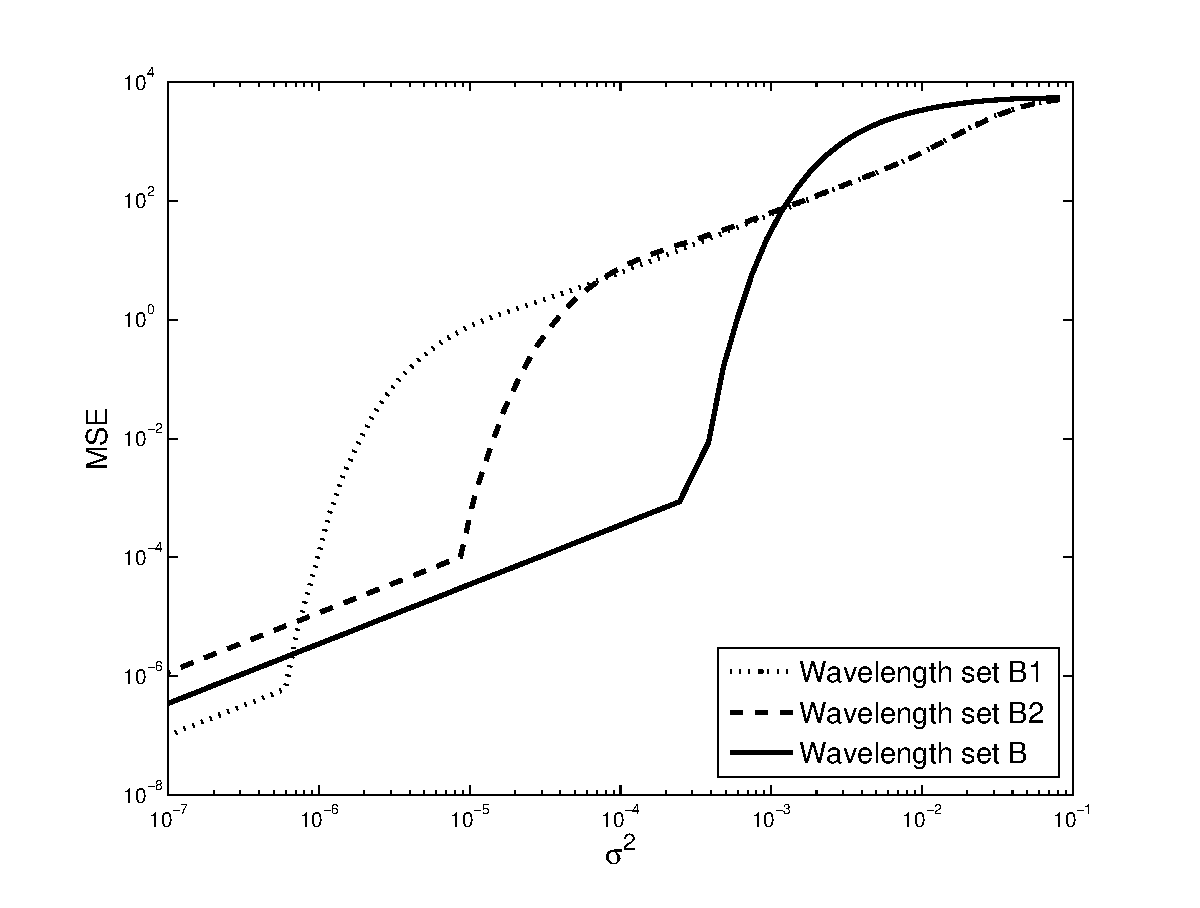
\includegraphics[scale=0.60]{code/data/Comparison_B1_B2_B.eps} 
% 		\caption{Effect of measurement wavelengths of the MSE curve.}     
% 		\label{fig:msecomparison}   
% \end{figure} 

%In Figure~{fig:benchmarks} we compare the computational complexity of the least squares range estimator with the CRT based range estimator. The computational complexity of the least squares range estimator (computed using a sphere decoder~\cite{Agrell2002}) grows exponentially with the number of wavelengths.  However, because the number of wavelengths is small in practice (we don't know of applications that use more than 10 wavelengths) computational complexity is not of serious concern. Figure~\ref{ch3:fig:benchmarks} shows the computation time required for the least squares estimator computed using a sphere decoder and the single stage CRT estimator of Xiao~et.~al.~\cite{Xiao_multistage_crt_2014} as the number of wavelengths $N$ increases.  The wavelengths are set to integers $\{1,2,3,\dots,N\}$ in each benchmark. In these benchmarks the least squares estimator is actually faster than the CRT for $N$ less than 38.  However, for large $N$ the sphere decoder becomes prohibitively expensive.
%
%
%\begin{figure}
%\centering
%  \begin{tikzpicture}
%    \selectcolormodel{gray} 
%    \begin{axis}[font=\footnotesize,ymode=log,height=11cm,width=14cm,xlabel={$N$},ylabel={time (ms)}, legend style={draw=none,fill=none,legend pos=north west,cells={anchor=west},font=\footnotesize}]
%      \addplot[mark= ] table {chapters/ch3/figs/LeastSquaresBenchmark};
%      \addplot[mark= ,dashed] table {chapters/ch3/figs/CRTBenchmark};
%      \legend{Least squares, CRT}
%   \end{axis}
%  \end{tikzpicture}  
% \caption{Computation time benchmark: Least squares estimator vs CRT estimator.}
% \label{ch3:fig:benchmarks}
%\end{figure} 



% The computational complexity mainly depends on the closest lattice point algorithm. This paper employs sphere decoder whereas \cite{Li_distance_est_wrapped_phase} used Babi's algorithm to find the closest lattice point.  As the number of wavelengths used in practical systems are usually less than ten (e.g. two for GPS) the sphere decoder's complexity is close to  the Babai's algorithm for low dimensions (less than ten). Furthermore, it has been noted that the proposed algorithm is faster than the CRT method proposed in~\cite{Xiao_multistage_crt_2014}.


 \section{Summary}
%In this chapter, we considered the problem of estimating the range (or distance) between two locations using the phase of arrival method which provides the most accurate range estimates in many applications. A difficulty with phase of arrival is that only the principal component of the phase can be observed. This limits the range that can be unambiguously estimated to the wavelength of the signal. This problem is addressed by utilising signals of multiple different wavelengths and observing the phase at each. 

In this chapter we have considered least squares/maximum likelihood estimation of range from observation of phase at multiple wavelengths. We showed that the least squares range estimator can be computed by solving a problem from computational number theory known as the~\emph{closest lattice point problem}. Efficient general purpose algorithms for computing a closest lattice point require a~\emph{basis} for the lattice.  Constructing a basis for the least squares estimator of range is non-trivial. Bases have previously been constructed under the assumption that the wavelengths can be scaled to relatively prime integers.  In this chapter, interesting properties of lattices generated by intersection with or projection onto a subspace are used to construct a basis in the general case. Furthermore, the basis construction method provided in this research is simpler than the existing method provided in~\cite{Li_distance_est_wrapped_phase}. 

The construction of basis for the general case is important because the accuracy of the range estimator depends upon the wavelengths. Simulations indicate that this can dramatically improve range estimates.  These results lead to important problems of characterising the dependence of the least squares range estimator upon the measurement wavelengths and selecting wavelengths to maximise the accuracy of the least squares estimator that is addressed in the following chapters.







%%%%%%%%%%%%%%%%%%%% Chapter 4 - Fast Convergence rate Routing %%%%%%%%%%%%%%%%%%%%%%%%%%%%%%%%%%%%%%%%%%%%%
%\setcounter{mtc}{12}
\chapter{Robustness of the Least Squares Range Estimator}
%\minitoc
%\newpage
\graphicspath{{./}{chapters/ch4/}}
\label{Chapter4}
 \setstretch{1.5}

\section{Introduction}\label{ch4:sec:Introduction}

%Range (or distance) estimation is important in various localization systems such as global positioning system (GPS)~\cite{Teunissen_GPS_LAMBDA_2006,Teunissen_GPS_1995} and electronic surveying~\cite{Jacobs_ambiguity_resolution_interferometery_1981, anderson1998surveying}. Among various available methods for range estimation, phase of arrival based methods provide the most accurate estimates of the range. However, this method inherits the problem of \emph{phase ambiguity}. Phase ambiguity problem occurs due to an inherent property of the phase that the observed value of the phase is always in the range $[-\pi, \pi)$. This phase ambiguity problem occurs when the unknown range is larger than the wavelength of the signal. This problem is addressed by using multiple different frequencies at the transmitter and observing the phase at each. The range can then be measured within an interval of length equal to the lcm of the wavelengths~\cite{Xiaowei_Li_robust_CRT_2009, W.Wang_closed_form_crt_2010, Li_distance_est_wrapped_phase,Akhlaq_basis_construction_range_est_2015}.
%
%One solution to this problem is based on the Chinese remainder theorem (CRT) when the wavelengths can be scaled to pairwise relatively prime integers. CRT based range estimators are also proposed when the wavelengths can not be scaled to pairwise relatively prime integers~\cite{Oystein_Ore_general_chinese_Remainder_1952, Yuke_new_CRT_1998}. However, it is well known that CRT based range estimators are not robust i.e. a small error in the remainder may produce a large error in the estimated solution. Both approximate and exact techniques for computing the least squares range estimator and related estimators have also been studied by Teunissen~\cite{Teunissen_GPS_1995}, Hassibi and Boyd~\cite{Hassibi_GPS_1998}, Xiaoet~al.~\cite{Li_distance_est_wrapped_phase, Li_coloured_2013} and most recently by Assad~et~al.~\cite{Akhlaq_basis_construction_range_est_2015}.  

%Range (or distance) estimation is an important component of modern technologies such as electronic surveying~\cite{Jacobs_ambiguity_resolution_interferometery_1981, anderson1998surveying} and global positioning~\cite{Teunissen_GPS_LAMBDA_2006,Teunissen_GPS_1995}.  Common methods of range estimation are based upon received signal strength~\cite{Chitte_RSS_Estimation2009, HingCheung_RSSbasedRangeEstimation2012}, time of flight (or time of arrival)~\cite{XinrongLi_TOA_range_estimation2004, Lanzisera_TOA_range_estimation2011}, and phase of arrival~\cite{Jacobs_ambiguity_resolution_interferometery_1981,Towers_frequency_selection_interferometry_2003,Li_distance_est_wrapped_phase}.  This paper focuses on the phase of arrival method which provides the most accurate range estimates in many applications.  Phase of arrival has become the technique of choice in modern high precision surveying and global positioning ~\cite{Odijk-nteger-ambiguity-resolutionPPP, Teunissen_GPS_LAMBDA_2006, Teunissen_GPS_1995}. 
%
%A difficulty with phase of arrival is that only the principal component of the phase can be observed.  This limits the range that can be unambiguously estimated.  One approach to address this problem is to utilise signals of multiple different wavelengths and observe the phase at each.  The range can then be measured within an interval of length equal to the least common multiple of the wavelengths.  Range estimators from such observations have been studied by numerous authors~\cite{Teunissen_GPS_1995,Hassibi_GPS_1998,Towers_frequency_selection_interferometry_2003,Towers:04_generalised_frequency_selection,Li_distance_est_wrapped_phase, Xia2007, XWLi2008,Xiao_multistage_crt_2014}.  Techniques include the beat wavelength method of Towers~et~al.~\cite{Towers_frequency_selection_interferometry_2003,Towers:04_generalised_frequency_selection}, the method of excess fractions~\cite{Falaggis_excess_fractions_2013}, and methods based on the Chinese Remainder Theorem (CRT)~\cite{Oystein_Ore_general_chinese_Remainder_1952,Yuke_new_CRT_1998, Oded_Chinese_remaindering_with_errors_2000, G.Wang_location_and_imaging_2004, Xia_generalised_CRT_2005, Xia2007, XWLi2008, Xiaowei_Li_robust_CRT_2009, W.Wang_closed_form_crt_2010, Xiaowei_Li_location_and_imaging_2011, YangBin_range_estimation_with_CRT_2014, Xiao_multistage_crt_2014}.  Least squares/maximum likelihood and maximum a posteriori estimators of range have been studied by Teunissen~\cite{Teunissen_GPS_1995}, Hassibi and Boyd~\cite{Hassibi_GPS_1998}, and more recently by Li~et~al.~\cite{Li_distance_est_wrapped_phase} and Akhlaq~et~al.~\cite{Akhlaq_basis_construction_range_est_2015}.  A key realisation is that the least squares estimator can be efficient computed by solving a well known integer programming problem, that of computing a \emph{closest point} in a \emph{lattice}~\cite{Agrell2002}.    Teunissen~\cite{Teunissen_GPS_1995} appears to have been the first to have realised this connection.
 


All of the range estimators such as beat wavelength, excess fractions, CRT and least squares either explicitly, or implicitly, make an estimate of so called integer \emph{wrapping variables} related to the whole number of wavelengths that occur over the range.  Given estimates of the wrapping variables, an estimate of the range is typically given by linear regression.  It is expected that accurate estimators of the wrapping variables will also be accurate estimators of the range. Identification of a criterion that guarantees the correctness of these wrapping variables for the least squares range estimator is important because it provides a basis for selecting wavelengths/frequencies to be used for range estimation. In this chapter we first define the \emph{wrapping variables} and then find a condition on the phase measurement errors that guarantees the correctness of these variables. This finding further motivates the search for methods of selecting wavelengths that can maximise the probability of correctness of these wrapping variables, which is the focus of next chapter.

Robust range estimators from erroneous phase measurements (remainders) for CRT based range estimators are proposed in~\cite{Xiaowei_Li_robust_CRT_2009, W.Wang_closed_form_crt_2010} . They derived an upper bound $\taucrt$ such that if all the absolute phase measurement errors are less than $\taucrt$, then the CRT estimator is guaranteed to correctly estimate the wrapping variables. They called $\taucrt$ the \emph{robustness bound}. Their robustness bound holds only if the greatest common divisor (gcd) of all the wavelengths is greater than one and the remaining wavelengths after division by this gcd are co-prime. Recently a robust CRT based range estimator was also proposed in~\cite{Xiao_multistage_crt_2014} for the general case without the constraint used in ~\cite{Xiaowei_Li_robust_CRT_2009, W.Wang_closed_form_crt_2010}. 

In this chapter we derive a similar upper bound $\tauls$ for the least squares range estimator that indicates the superior performance of the least squares range estimator compared to the CRT estimator.  If all absolute phase measurement errors are less than $\tauls$, then the least squares range estimator is guaranteed to correctly estimate the wrapping variables.  The bound is derived from a lattice property called the \emph{inradius}.  We find that  $\tauls > \taucrt$ in many cases.  This corroborates with existing empirical evidence suggesting that the least squares estimator is often more accurate than those estimators based on the CRT~\cite{Akhlaq_basis_construction_range_est_2015}.

The chapter is organised as follows. Section \ref{ch4:sec:phase-and-range-relation} presents the concept of correct wrapping variables.  Section \ref{ch4:sec:robustness-bound} derives our upper bound $\tauls$ for the least squares range estimator based upon the inradius of a lattice.  Section \ref{ch4:sec:sim-results} compares the proposed bound $\tauls$ with the bound $\taucrt$ for the CRT based estimator of Xiao~et~al.~\cite{Xiao_multistage_crt_2014}.  We find that $\tauls > \taucrt$ in many cases.  The results of Monte-Carlo simulations are presented and it is found that the bounds $\tauls$ and $\taucrt$ provide insight about the mean square error of these range estimators.

%**************************************************************************************************************************************************************
%		Section II :  System Model
%**************************************************************************************************************************************************************
\section{Concept of Correct Wrapping Variables}\label{ch4:sec:phase-and-range-relation}
%Suppose that a transmitter sends a sinusoidal signal 
%\[
%s(t)=  \sin (2\pi ft + 2\pi\phi)
%\] 
%with known phase $\phi$. The signal is assumed to propagate by line of sight to a receiver resulting in the signal 
%\[
%y(t) = \alpha s(t - r_0/c) + \omega(t) = \alpha \sin (2\pi ft + 2\pi\theta) +  \omega(t)
%\]
%where $r_0$ is the distance (or range) between the transmitter and the receiver, $c$ is the speed at which the signal propagates, $\alpha$ is the amplitude of the received signal, and $\omega(t)$ represents noise. The phase of the received signal is
%\[
%\theta = \phi - \dfrac{ f }{c}r_0 = \phi - \dfrac{r_0}{\lambda}
%\]
%where $\lambda = c/f$ is the wavelength. In order to estimate the range $r_0$ the receiver first makes an estimate $\hat{\theta} \in [-\tfrac{1}{2}, \tfrac{1}{2})$ of the principal component of the phase $\theta$. The range $r_0$ is related to the phase estimate $\hat{\theta}$ by the phase difference
%\begin{equation*}
%Y = \sfracpart{\phi - \hat{\theta}} = \fracpart{ r_0/\lambda + \Phi },
%\end{equation*}
%where $\Phi$ represents phase noise and $\sfracpart{x} = x - \round{x}$ denotes the \emph{centered} fractional part of $x$, where $\round{x}$ is the  closest integer to $x$ with half integers rounded up. Observe that ranges $r_0$ and $r_0 + k\lambda$ for any integer $k$ result in the same  phase difference $Y$.  For this reason, the range is identifiable from the phase difference only if we assume $r_0$ to lie in some interval of length $\lambda$.  
%%, or more generally, in some set of coset representatives of the quotient group $\reals / \lambda\ints$.  
%A natural choice is the interval $[0, \lambda)$.
%
%This poses a problem if the range $r_0$ is larger than the wavelength $\lambda$.  A common approach to address this problem is to transmit multiple signals at multiple different frequencies and observe the phase at each. In this approach, $N$ phase estimates $\hat{\theta}_1,\ldots,\hat{\theta}_N$ and $N$ phase differences 
%%\begin{equation}\label{eq:Yndefn}
%\begin{equation}\label{eq:Yndefn}
%Y_n = \sfracpart{\phi - \hat{\theta}_n} = \fracpart{ r_0/\lambda_n + \Phi_n}, \qquad n = 1, \dots, N
%%& = \fracpart{ r_0/\lambda_n + X_n} \qquad n = 1,\dots,N 
%%& = r_0/\lambda_n + X_n - z_{0n}
%\end{equation}
%%\end{equation}
%are computed, where $\lambda_n = c/f_n$ is the wavelength of the $n$th signal and $\Phi_1,\dots,\Phi_n$ represent phase noise.  Let $P = \lcm(\lambda_1,\dots,\lambda_N)$ be the least common multiple of the wavelengths.  The least common multiple is the smallest postive integer such that $P/\lambda_1, \dots, P/\lambda_N$ are all integers.  Observe that the ranges $r_0$ and $r_0 + kP$ for any integer $k$ result in the same phase differences $Y_1,\dots,Y_N$ and so $r_0$ can be uniquely identified only within an interval of length $P$.  A natural choice is the interval $[0,P)$.  The least common multiple $P$ is typically much larger than any individual wavelength and so the identifiable range can be considerably enlarged by the use of multiple wavelengths.   If $\lambda_n/\lambda_m$ is irrational for any $n$ and $m$ then the least common multiple $P$ does not exist.  In this paper we assume this is not the case and that a finite least common multiple $P$ does exist.  This is a common assumption in the literature and in practice.  %In what follows we will call the ranges $r_0$ and $r_0 + kP$ as 
%
In this section, we further extend the system model presented in~\ref{ch3:sec:ls-estimator} and define the correct wrapping variables. The understanding of correct wrapping variables is necessary to define the bound $\tauls$ for the least squares range estimator in the next section. Recall that the phase differences can be written in the form 
\begin{align*}
Y_n &=  \fracpart{ r_0/\lambda_n + \Phi_n} =  r_0/\lambda_n + \Phi_n + \zeta_n
\end{align*}
where the integers
\[
\zeta_n = -\round{r_0/\lambda_n + \Phi_n} \qquad n = 1 ,\dots, N 
\]
are called \emph{wrapping variables}. The wrapping variables are related to the number of whole wavelengths that occur over the range $r_0$ between the transmitter and the receiver.  Writing in column vector form
\begin{equation}\label{ch4:eq:Yndefn_vecform}
\ybf = r_0\wbf + \Phibf + \zetabf
\end{equation}
where the column vectors
\[
\ybf = \left(\begin{matrix} Y_1 \\ \vdots \\ Y_N \end{matrix}\right)  \;\; 
\zetabf = \left( \begin{matrix} \zeta_1 \\ \vdots \\ \zeta_N \end{matrix}\right) \;\;
\wbf = \left( \begin{matrix} \frac{1}{\lambda_1} \\ \vdots \\ \frac{1}{\lambda_N} \end{matrix} \right) \;\; 
\Phibf = \left( \begin{matrix} \Phi_1 \\ \vdots \\ \Phi_N \end{matrix} \right) .
\]
%\begin{align*}
%\ybf &= (Y_1,\dots,Y_N)^\prime \in \reals^N, \\
%\zetabf &= (\zeta_1,\dots,\zeta_N)^\prime \in \ints^N, \\
%\wbf &= \left(1/\lambda_1,\dots,1/\lambda_N\right)^\prime \in \reals^N , \\
%\Phibf &=(\Phi_1,\dots,\Phi_N)^\prime \in \reals^N.
%\end{align*}
The $n$th element of the vector $\wbf$ is the reciprocal of the $n$th wavelength, that is, $w_n = 1/\lambda_n$.  Observe $P$ is the smallest positive number such that the vector 
\[
\vbf = P\wbf = (P/\lambda_1, \dots, P/\lambda_N) \in \ints^N,
\]
that is, such that the elements of $\vbf = P\wbf$ are all integers. Equivalently, $P$ is the unique positive real number such that the elements of $\vbf$ are jointly relatively prime, that is, such that 
\[
\gcd(v_1,\dots,v_N) = \gcd(P/\lambda_1, \dots, P/\lambda_N) = 1.
\]
Common range estimators, such as the least squares estimator, those estimators based on the CRT, and the method of excess fractions, operate in two stages. In the first stage, an estimate $\hat{\zetabf}$ of the wrapping variables $\zetabf$ is made. Given $\hat{\zetabf}$, an estimate of the range $r_0$ is typically given by linear regression, that is, 
%\begin{equation}\label{betahatz}
\begin{equation}\label{ch4:eq:rhatlinreg}
\hat{r}  = \frac{(\ybf - \hat{\zetabf})^\prime\wbf}{\wbf^\prime\wbf}
\end{equation}
%\end{equation}
where superscript $^\prime$ indicates the vector or matrix transpose. For any integer $k$, the ranges $r_0$ and $r_0 + kP$ are equivalent and so the range estimates $\hat{r}$ and $\hat{r} + kP$ for any integer $k$ are equivalent.  % To account for this, the least squares range estimator is given by~\cite[Eq.~(6)]{Akhlaq_basis_construction_range_est_2015}
% \begin{equation}\label{hatrangeLS}
% \hat{r}_{\text{LS}}  = \hat{r} - P \floor{\hat{r}/P}.
% \end{equation}
It follows that estimates $\hat{\zetabf}$ and $\hat{\zetabf} + kP\wbf$ of the wrapping variables are equivalent, because
\[
\frac{(\ybf - \hat{\zetabf} + kP\wbf)^\prime\wbf}{\wbf^\prime\wbf} = \hat{r} + kP.
\]
For this reason, the estimated wrapping variables $\hat{\zetabf}$ are to be considered error free (or correct), if $\hat{\zetabf} = \zetabf + kP\wbf$ for some integer $k$.  Because $P$ is the smallest positive integer such that $\vbf = P\wbf \in \ints^N$ this occurs if and only if $\Qbf \hat{\zetabf} = \Qbf \zetabf$ where 
\begin{equation}\label{eq:Qproj}
\Qbf = \Ibf - \frac{\wbf\wbf^\prime}{\wbf^\prime\wbf} = \Ibf - \frac{\vbf\vbf^\prime}{\vbf^\prime\vbf}
\end{equation}
is the $N \times N$ orthogonal projection matrix onto the $N-1$ dimensional subspace orthogonal to $\wbf$ and $\Ibf$ is the $N\times N$ identity matrix.  In what follows, estimates $\hat{\zetabf}$ of the wrapping variables $\zetabf$ are said to be \emph{correct} if $\Qbf \hat{\zetabf} = \Qbf \zetabf$.

Xiao~et~al.~\cite{Xiao_multistage_crt_2014} derived an upper bound 
\begin{equation}\label{eq:crt-upper-bound}
\tau_{_{CRT}} =  \frac{1}{4c \lambda_{\max}}\min_{1\leq i \leq N}  \min_{1\leq j \neq i \leq N} \gcd (c\lambda_i, c\lambda_j)
\end{equation} 
such that if the absolute values of the phase noise are less than $\taucrt$, then the CRT estimator is guaranteed to correctly estimate the wrapping variables.  That is, if  $\abs{\Phi_n} < \taucrt$ for all $n = 1, \dots, N$, then $\Qbf \hat{\zetabf} = \Qbf\zetabf$.  The value $\lambda_{\text{max}} = \max_n \lambda_n$ is the maximum wavelength and $c$ is a positive real number such the scaled wavelengths $c \lambda_1, \dots, c \lambda_N$ are all integers.  The existance of $c$ is guaranteed by the fact that the wavelengths are assumed to be rationally related, that is, $\lambda_n/\lambda_k$ is rational for all $n$ and $k$.

In the next section we will find a similar upper bound $\tauls$ for the least squares range estimator.  It is shown in \Sec{ch3:sec:range-estim-clos-1}, that the least squares estimator $\hat{\zetabf} \in \ints^N$ of the wrapping variables minimises the quadratic form
\begin{equation}\label{eq:hatz}
\| \Qbf\ybf - \Qbf\zbf \|^2 \qquad \text{over $\zbf \in \ints^N$},
\end{equation}
where $\|\cdot\|$ indicates the Euclidean norm of a vector.  Given $\hat{\zetabf}$, the least square range estimator $\hat{r}$ is then given by~\ref{ch4:eq:rhatlinreg}.  It is shown in \Sec{ch3:sec:range-estim-clos-1} how the quadratic form~\ref{ch3:eq:hatz} can be minimised over $\ints^N$ by computing a closest point in a \emph{lattice}.  We will derive the bound $\tauls$ by using a property of this lattice from \Sec{sec:ch2-lattice-theory} called the \emph{inradius}. 

%It is shown in~\cite{Akhlaq_basis_construction_range_est_2015}, that the least squares estimate $\hat{\zetabf} \in \ints^N$ of the wrapping variables minimises the quadratic form
%\begin{equation}\label{eq:hatz}
%\| \Qbf\ybf - \Qbf\zbf \|^2 \qquad \text{over $\zbf \in \ints^N$},
%\end{equation}
%where $\|\cdot\|$ indicates the Euclidean norm of a vector.  It is shown in~\cite{Akhlaq_basis_construction_range_est_2015} how this quadratic form can be minimised over $\ints^N$ by computing a closest point in a lattice.  We will derive the bound $\tauls$ by studying a property of this lattice called the \emph{inradius}.  We first require some introductory concepts from lattice theory.

% If we denote this subspace by $H$ then by~\cite[Corollary 1]{Akhlaq_basis_construction_range_est_2015} the set $\Lambda = \ints^N \cap H$ and the set $\Lambda^* = \{ \Qbf \zbf \mid \zbf \in \ints^N \}$.  We see that the problem of minimising~\eqref{eq:hatz} is precisely that of finding a closest lattice point in $\Lambda^*$ to $\Qbf\ybf \in \reals^N$.  
% A solution to~\eqref{eq:hatz} is provided in~\cite{Akhlaq_basis_construction_range_est_2015} by solving a problem from computational number theory called the closest lattice point~\cite{Agrell2002}. Given estimates $\hat{\zetabf}$ of the wrapping variables  the least squares estimate of $r_0$ is given as~\cite{Akhlaq_basis_construction_range_est_2015}


%**************************************************************************************************************************************************************
%		Section III :  Lattice theory
%**************************************************************************************************************************************************************
%\section{Lattice theory}\label{ch4:sec:lattice-theory}
%
%Let $\mathbf{b}_1,....,\mathbf{b}_n$ be linearly independent vectors from $m$-dimensional Euclidean space $\reals^m$ with $m\geq n$.  The set of vectors
%\[
%\Lambda = \{ u_1\bbf_1 + \dots + u_n \bbf_n \mid u_1,\dots,u_n \in \ints \}
%\]
%is called an $n$-dimensional \term{lattice}.  The elements of $\Lambda$ are called \term{lattice points} or \term{lattice vectors}. 
%The vectors $\bbf_1,\dots,\bbf_n$ form a \emph{basis} for the lattice $\Lambda$.  We can equivalently write
%\[
%\Lambda=\{ \Bbf\ubf \mid \ubf \in \ints^n \}
%\]
%where $\Bbf$ is the $m\times n$ matrix with columns $\bbf_1,\dots,\bbf_n$. The matrix $\Bbf$ is called a \term{basis} or \term{generator} for $\Lambda$. When $m = n$ the lattice is said to be \term{full rank}. When $m > n$ the lattice points lie in the $n$-dimensional subspace of $\reals^m$ spanned by $\bbf_1,\dots,\bbf_n$.  %The set of integers $\ints^n$ is called the \term{integer lattice} with the $n \times n$ identity matrix $\bf{I}$ as a basis.
%
%%The parallelepiped formed by basis vectors $\bbf_1,\dots,\bbf_n$ is called a \term{fundamental parallelepiped} of the lattice $\Lambda$.  A fundamental parallelepiped has $n$-dimensional volume $\sqrt{\det \Bbf^\prime\Bbf }$ where superscript $^\prime$ denotes the vector or matrix transpose.  This quantity is also called the determinant of the lattice and is denoted by $\det\Lambda$.  
%The (closed) \term{Voronoi cell}, denoted $\vor\Lambda$, of an $n$-dimensional lattice $\Lambda$ in $\reals^m$ is the subset of $\reals^m$ containing all points nearer or of equal distance (here with respect to the Euclidean norm) to the lattice point at the origin than to any other lattice point (Figure~\ref{fig:bound_dmin}).  % Equivalently, the Voronoi cell can be defined as the intersection of the half spaces 
%% \begin{align*}
%% H_{\wbf} &= \{\xbf \in \reals^n \mid \|\xbf\| \leq \|\xbf - \wbf\| \} \\
%% &= \{\xbf \in \reals^n \mid \dotprod{\xbf}{\wbf} \leq \tfrac{1}{2}\dotprod{\wbf}{\wbf} \}
%% \end{align*}
%% for all $\wbf \in \Lambda \backslash  \{\zerobf\}$ where $\Lambda \backslash  \{\zerobf\}$ denotes the set of lattice points not equal to the origin $\zerobf$.
%The Voronoi cell $\vor\Lambda$ tesselates $\reals^N$ in the sense that
%\[
%\reals^N = \bigcup_{\xbf \in \Lambda} (\vor\Lambda + \tbf)
%\]
%and $\vor\Lambda$ and a translate $\vor\Lambda + \tbf$ by a lattice point $\tbf \in \Lambda\backslash  \{\zerobf\}$ intersect at most on the boundary of $\vor\Lambda$.  The set $\Lambda \backslash  \{\zerobf\}$ denotes those lattice points from $\Lambda$ not equal to the origin $\zerobf$.  In particular, if $\interior\Lambda$ denotes the interior of the Voronoi cell, then the intersection of $\interior\Lambda$ and $\vor \Lambda + \tbf$ is empty for all $\tbf \in \Lambda \backslash  \{\zerobf\}$.  % Equivalently, if $\tbf \in \Lambda$, $\wbf \in \vor\Lambda$, and $\ybf \int\Lambda$, and
%% \[
%% \]
%This leads to the following simple property that we will find useful.
%
%\begin{remark}\label{remarksimpleintvor}
%If $\tbf \in \Lambda$, $\ubf \in \vor\Lambda$, $\vbf \in \interior\Lambda$, and $\ubf = \vbf + \tbf$, then $\tbf = \zerobf$.
%\end{remark}
%
%%Let $\Lambda$ be an $n$-dimensional lattice and let $H$ be the $n$-dimensional subspace spanned by its lattice points. The \term{dual lattice} of $\Lambda$, denoted $\Lambda^*$, contains those points from $H$ that have integer inner product with all points from $\Lambda$, that is,
%%\[
%%\Lambda^* = \{ \xbf  \in H \mid \xbf^\prime \ybf \in \ints \text{ for all } \ybf \in \Lambda \}.
%%\] 
%% 
%Given a vector $\ybf \in \reals^m$, a problem of interest is to find a lattice point $\xbf \in \Lambda$ such that the squared Euclidean norm
%\[
%\| \ybf - \xbf \|^2 = \sum_{i=1}^m (y_i - x_i)^2 
%\]  
%is minimised.  This is called the \term{closest lattice point problem} (or \term{closest vector problem}) and a solution is called a \term{closest lattice point} (or simply \term{closest point}) to $\ybf$ \cite{Agrell2002,McKilliam2009CoxeterLattices,MicciancioVoulgaris_deterministic_jv_2013,McKilliam_closest_point_lattice_first_kind_2014}.  The closest lattice point problem and the Voronoi cell are related in that $\xbf\in\Lambda$ is a closest point to $\ybf$ if and only if $\ybf - \xbf \in \vor\Lambda$. 
%
%A \emph{short vector} in a lattice $\Lambda$ is a lattice point of minimum nonzero Euclidean length, that is, a lattice point of length
%\[
%\dmin =  \min_{\xbf \in \Lambda \backslash \{ \zerobf \} } \| \xbf \|^2.
%\]   
%The length $\dmin$ of a short vector is the smallest distance between any two lattice points.  The \emph{inradius} or \emph{packing radius} $\rho = \dmin/2$ is the length of a point on the boundary of the Voronoi cell that is closest to the origin (Figure~\ref{fig:bound_dmin}).  Equivalently, the inradius is the radius of the largest sphere that fits inside the Voronoi cell.  It is also the radius of the largest sphere that can be centered at each lattice point such that no two spheres intersect.  Such an arrangement of spheres is called a \emph{sphere packing} (Figure~\ref{fig:bound_dmin}).
%
%% For a given lattice $\Lambda$ with generator matrix $\mathbf{B}$, the minimum distance of the lattice or the length shortest lattice vector $d_{\min}$ is defined as 
%  
%%  \[
%%  d_{\min} = \underset{\zbf \in \mathbf{\ints}^n , \zbf\neq 0}{\operatorname{min}} \|\mathbf{Bz} \|. 
%%  \]
%%  $d_{\min}$ is the length of the shortest lattice vector other than origin i.e. it is the distance between the origin and its closest lattice point as shown in Figure~\ref{fig:bound_dmin}. The inradius of a lattice is equal to the half of the length of the shortest lattice vector i.e. $\frac{d_{\min}}{2}$.
% 
%\begin{figure}[t]
%\begin{center} 
%%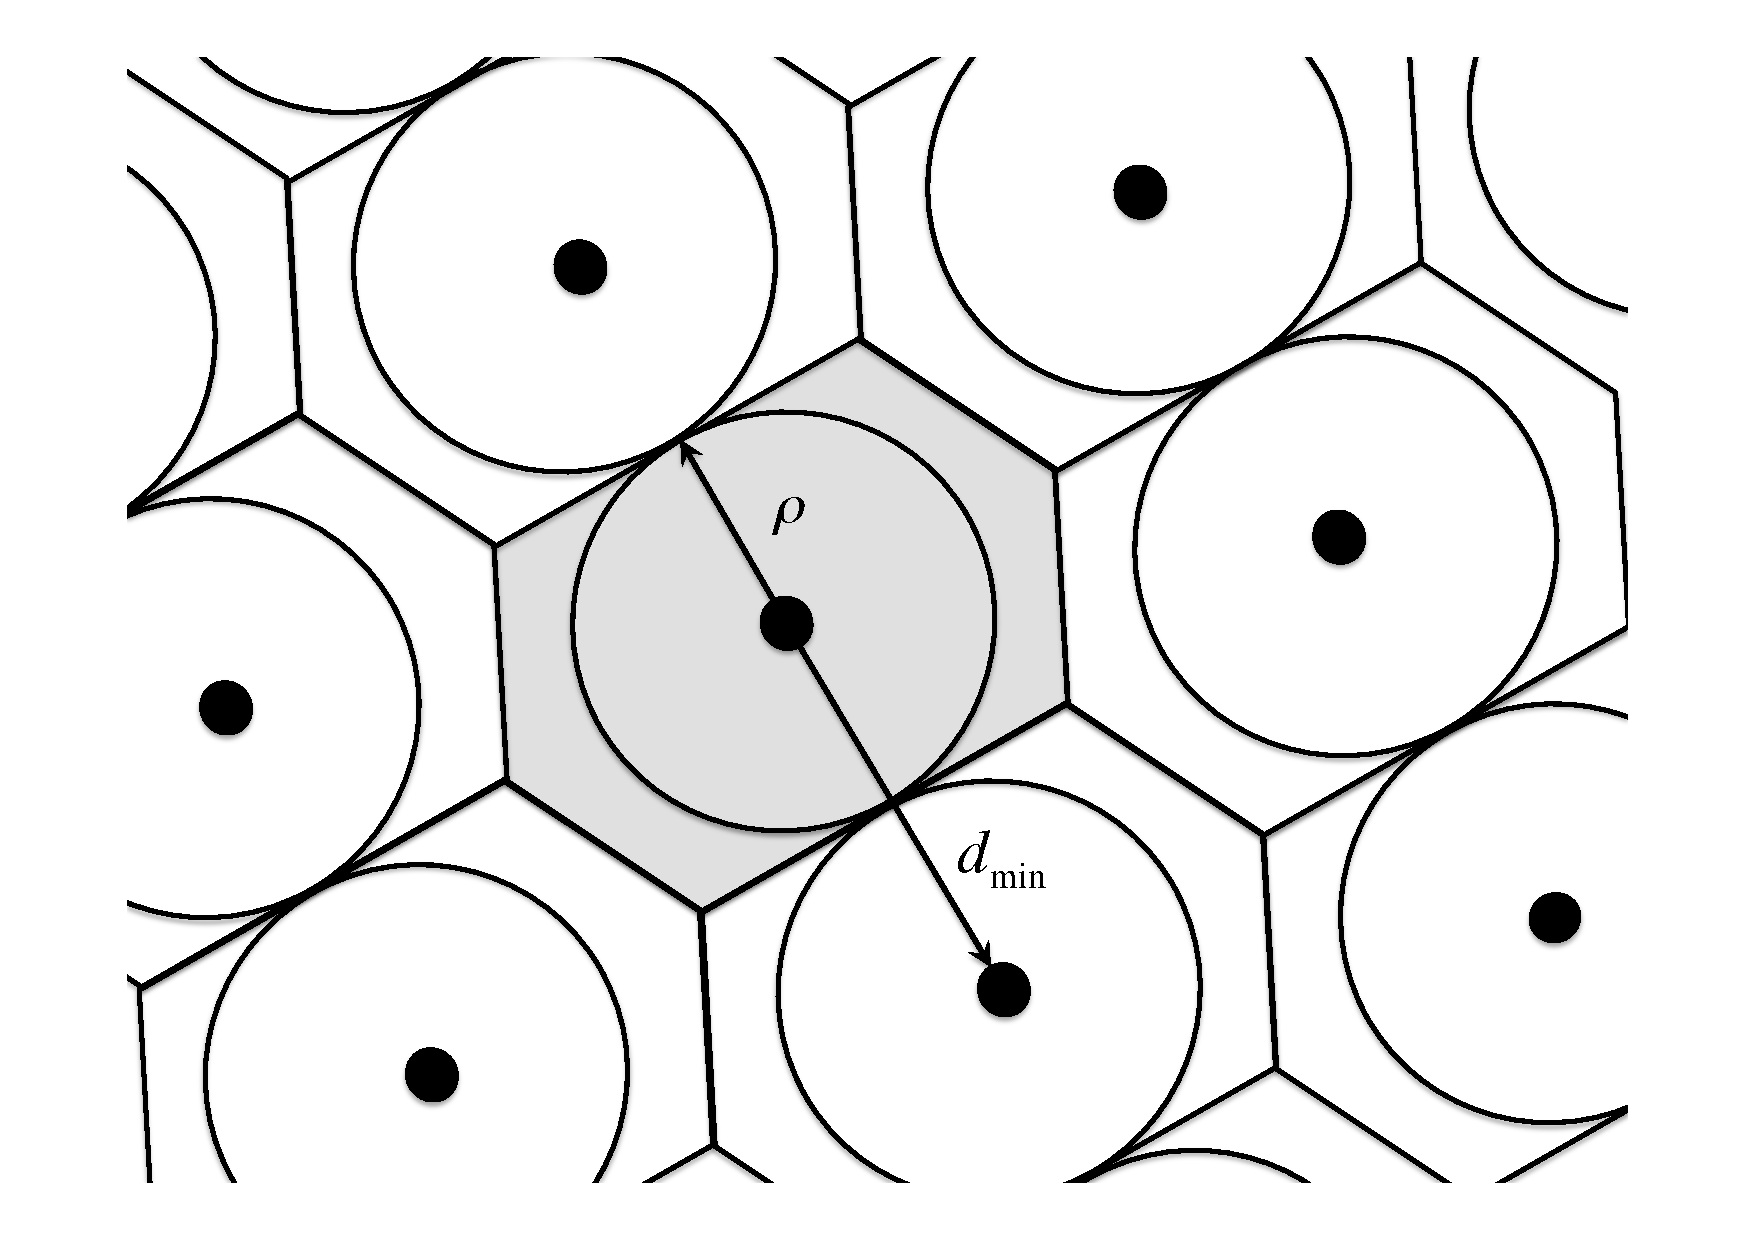
\includegraphics[scale=0.30]{figs/bound_dmin.pdf} 
%%\caption{The length of a short vector $\dmin$ and inradius $\rho = \dmin/2$ of the 2-dimensional lattice. This lattice has two short vectors. The shaded region shows the Voronoi cell of the lattice. The circles exhibit a sphere packing.}
%\includegraphics{chapters/ch4/Figs/latticefigures-1.mps}
%\caption{The length of a short vector $\dmin$ and inradius $\rho = \dmin/2$ of the 2-dimensional lattice with basis $\bbf_1 = [3,0.6]^\prime, \bbf_2 = [0.6,3]^\prime$. This lattice has four short vectors.  The shaded region shows the Voronoi cell of the lattice.  The circles exibit a sphere packing.}
%\label{fig:bound_dmin}
%\end{center}  
%\end{figure} 
%  
%**************************************************************************************************************************************************************
%		Section IV : Criterion for robust range estimation
%**************************************************************************************************************************************************************
\section{Bound for the least squares range estimator}\label{ch4:sec:robustness-bound}

Recall that the least squares estimate $\hat{\zetabf}$ of the wrapping variables $\zetabf$ minimises the quadratic form $\|\Qbf \ybf - \Qbf \zbf\|^2$ over $\zbf \in \ints^N$, that is,
\[
\|\Qbf \ybf - \Qbf \hat{\zetabf}\|^2 = \min_{\zbf \in \ints^N} \|\Qbf \ybf - \Qbf \zbf\|^2.
\]
It is shown in~\refchapter{Chapter3} that the set
\[
\Lambda^* = \{ \Qbf\zbf \mid \zbf \in \ints^N  \}
\]
is an $N-1$ dimesional lattice.  Thus, $\Qbf\hat{\zetabf}$ is a lattice point in $\Lambda^*$ and, because 
\begin{align*}
\|\Qbf \ybf - \Qbf \hat{\zetabf}\|^2 &= \min_{\zbf \in \ints^N} \|\Qbf \ybf -  \Qbf \zbf\|^2 \\
&= \min_{\xbf \in \Lambda^*} \|\Qbf \ybf - \xbf\|^2,
\end{align*}
it follows that $\Qbf \hat{\zetabf}$ is a closest lattice point to $\Qbf\ybf$.  Because of this, $\Qbf \ybf - \Qbf \hat{\zetabf}$ is an element of the Voronoi cell of the lattice $\Lambda^*$, that is,
\[
\Qbf \ybf - \Qbf \hat{\zetabf} = \Qbf ( \ybf -  \hat{\zetabf} ) \in \vor \Lambda^*.
\]
Observe from~\ref{ch4:eq:Yndefn_vecform} that
\begin{align*}
\Qbf (\ybf - \hat{\zetabf}) &= \Qbf (r_0\wbf + \Phibf + \zetabf - \hat{\zetabf}) \\
&= \Qbf \Phibf - \Qbf(\zetabf - \hat{\zetabf}).
\end{align*}
Suppose that the projection of the phase noise $\Qbf \Phibf$ is in the interior of the Voronoi cell $\interior \Lambda$.  Then, it follows from Remark~\ref{remarksimpleintvor} of~\refchapter{Chapter2}, with $\tbf = \Qbf(\zetabf - \hat{\zetabf})$, $\ubf = \Qbf (\ybf - \hat{\zetabf})$, and $\vbf = \Qbf \Phibf$, that $\Qbf(\zetabf - \hat{\zetabf}) = \zerobf$ or equivalently $\Qbf\zetabf =\Qbf\hat{\zetabf}$.

We have found that the least squares estimate $\hat{\zetabf}$ of the wrapping variables is correct whenever the projection of the phase noise $\Phibf$ orthogonal to $\wbf$ is contained in the interior of the Voronoi cell, that is, if $\Qbf \Phibf \in \interior \Lambda$, then $\Qbf \hat{\zetabf} = \Qbf \zetabf$.  Let $\rho = \dmin/2$ be the inradius of the lattice $\Lambda^*$.  If $\|\Qbf \Phibf\| < \rho$ then $\Qbf \Phibf \in \interior \Lambda$ and so $\Qbf \hat{\zetabf} = \Qbf \zetabf$.  Becasue $\Qbf$ is an orthogonal projection matrix $\|\Phibf\| \geq \|\Qbf\Phibf\|$ and so 
\begin{align*}
&\|\Phibf\| < \rho \\
\implies &\|\Qbf\Phibf\| < \rho \\
\implies &\Qbf \hat{\zetabf} = \Qbf \zetabf,
\end{align*}
that is, the least squares estimate $\hat{\zetabf}$ of the wrapping variables is correct whenever the Euclidean norm of the phase noise is less than the inradius $\rho$ of the lattice $\Lambda^*$.  The inradius $\rho$ depends upon the lattice $\Lambda^*$ which in turn depends upon the wavelengths.  This naturally leads to the question of whether it is possible to select wavelengths that maximise the inradius.  This is an interesting and nontrivial problem that we intend to investigate in future research.


% For the least squares estimator we say that the wrapping variable $\hat{\zetabf}$ are correct if $\Qbf \zetabf = \Qbf \hat{\zetabf}$.  To see why this definition is valid, observe that $\hat{\zetabf} = \zetabf + a \wbf$ where $a$ is such that $a\wbf \in \ints^{N}$.  Because the least common multiple $P$ is the smallest positive number such that $P\wbf$ contains only integers, it follows that $a = kP$ for some integer $k$.  Now, the regression estimator of the range satisfies
% \[
% \hat{r} = \frac{(\ybf - \hat{\zetabf})^\prime\wbf}{\wbf^\prime\wbf} = \frac{(\ybf - \zetabf + kP\wbf)^\prime\wbf}{\wbf^\prime\wbf} = \frac{(\ybf - \zetabf)^\prime\wbf}{\wbf^\prime\wbf} + kP
% \]
% and, from~\eqref{hatrangeLS}, the least square estimator of the range is
% \[
% \hat{r}_{\text{LS}}  = \frac{(\ybf - \hat{\zetabf})^\prime\wbf}{\wbf^\prime\wbf} - P \floor{\hat{r}} = 
% \]

%In this section we provide a bound on phase errors to robustly estimate the wrapping variables, and hence the range, from multiple noisy phase observations. %\subsection{Estimating the wrapping variables}
%It can be observed from~\eqref{eq:Yndefn} that 
%\[
%\fracpart{Y_n - r/\lambda_n}^2 = (Y_n - r/\lambda_n - z_n)^2
%\]
%where $z_n$ $(n=1,\ldots, N)$ are often called \emph{wrapping variables}. These wrapping variables are related to the number of whole wavelengths that occur over the range $r_0$ between the transmitter and the receiver.
%In \cite{Akhlaq_basis_construction_range_est_2015}, we showed how the least squares range estimator $\hat{r}$  from \eqref{eq:hatdininterval} can be efficiently computed by computing a closest point in a lattice of dimension $N-1$. The wrapping variables $\zbf = [z_1,\ldots,z_n]'$ are obtained by minimising the function~\cite{Akhlaq_basis_construction_range_est_2015}
%\[
%F(\zbf) = \| \Qbf\ybf - \Qbf\zbf \|^2
%\]
%where $\Qbf = \Ibf - \wbf\wbf^\prime/\|\wbf\|^2$ is the orthogonal projection matrix onto the $N-1$ dimensional subspace orthogonal to $\wbf$. If we denote this subspace by $H$ then by~\cite[Corollary 1]{Akhlaq_basis_construction_range_est_2015} the set $\Lambda = \ints^N \cap H$ is an $N-1$ dimensional lattice with determinant $\|\wbf\|$ and dual lattice $\Lambda^* = \{ \Qbf \zbf \mid \zbf \in \ints^N \}$.  We see that the problem of minimising $F_2(\zbf)$ is precisely that of finding a closest lattice point in $\Lambda^*$ to $\Qbf\ybf \in \reals^N$.  
%
%Suppose we find $\hat{\xbf} \in \Lambda^*$ closest to $\Qbf \ybf$ and a corresponding $\hat{\zbf} \in \ints^N$ such that $\hat{\xbf} = \Qbf\hat{\zbf}$.  Then $\hat{\zbf}$ minimises $F_2$ and $\hat{\beta}(\hat{\zbf})$ minimises $F$.  The least squares range estimator in the interval $[0,P)$ is then
%\begin{equation}\label{eq:leastsquaresrangehatz}
%\hat{r} = P\big(\hat{\beta}(\hat{\zbf}) - \sfloor{\hat{\beta}(\hat{\zbf})}\big). %= P\left(\frac{(\ybf - \hat{\zbf})^\prime\wbf}{\wbf^\prime\wbf} - \floor{\frac{(\ybf - \hat{\zbf})^\prime\wbf}{\wbf^\prime\wbf}} \right)
%\end{equation}
%Let $V$ denotes the interior of the Voronoi cell $\vor\Lambda^*$. Note that $\hat{\zetabf}$ is a minimiser of $\| \Qbf (\ybf - \zbf) \|$ over $\zbf \in \ints^N$. %We say that the estimator is robust when $\hat{\zetabf}=\zetabf$.
% wrapping variables $\hat{\zbf}$ are ``correct'' if $\Qbf \hat{\zbf} = \Qbf \zbf_0$, that is, the estimates of the wrapping variables $\hat{\zbf}$ when the true range $r_0$ is known i.e. $\hat{\zbf}=\zbf_0$ . From~\eqref{eq:Yndefn}, we have
%\begin{align*}
%Y_n &= \fracpart{ r_0/\lambda_n + X_n} = \fracpart{ \beta_0 w_n + X_n} \\ %r_0/\lambda_n + X_n + z_{0n}\\
%&= \beta_0 w_n + X_n + z_{0n}
%\end{align*}
%where $r_0= P\beta_0 $, $w_n = P/\lambda_n$ and
%\[
%z_{0n} = -\round{\beta_0 w_n + X_n} = -\round{\dfrac{r_0}{\lambda_n} + X_n} 
%\]
% is the $n$th element of the vector $\zbf_0$. Observe that $\ybf - \zbf_0 = \beta_0 \wbf + \xbf$ because
%\[
%Y_n - z_{0n} = \fracpart{\beta_0 w_n +  X_n} + \round{\beta_0 w_n +  X_n} = \beta_0 w_n +  X_n
%\]
%where $\xbf = (X_1,\dots,X_N)^\prime$ is the column vector containing the phase noise. 
% Equivalently, $\Qbf (\ybf - \hat{\zetabf})$ is contained in the Voronoi cell $\vor\Lambda^*$. Now
% So  $\Qbf\zetabf = \Qbf\hat{\zetabf}$ only if $\Qbf\Phibf \in V$. In the following we provide an upper bound $\tau_{_{LS}}$ on phase errors such that $\Qbf\Phi$ is in $V$. This bound is based on the inradius of the lattice $\Lambda^*$. %It will be shown in the simulations results that the robustness bound obtained using the in-radius provides a better bound.

%\subsection{Upper bound $\tau_{_{LS}}$ on phase errors}

% Let $d_{\min}$ be the length of the shortest lattice vector in $\Lambda^*$ i.e. it is the distance between the origin and the closest lattice point in $\Lambda^*$. Then a sphere of radius $\rho = \tfrac{d_{\min}}{2}$ centred at the origin is the largest ball that lies inside $\vor\Lambda^*$ as shown in Figure \ref{fig:bound_dmin}. The radius $\rho$ is called the inradius of the Voronoi cell. Note that $\Qbf\hat{\zetabf} = \Qbf\zetabf$ when $\Qbf\Phi \in \vor\Lambda^*$, that is, $\Qbf\Phi$ lies inside a sphere of radius $\rho$ centred at the origin i.e.
%  \begin{equation}\label{eq-lowerbound-as-QPhi}
% % P_r(\Lambda,\sigma^2) \geq Pr(\|\xbf \| < \rho),
% \|\Qbf\Phi \| < \rho.
% \end{equation}
% As $\Qbf$ is the projection matrix it implies that $\| \Qbf\Phi \| \leq \| \Phi \|$. Therefore \eqref{eq-lowerbound-as-QPhi} is still satisfied if
%  \begin{equation}\label{eq-lowerbound-as-Phi}
% \|\Phi \|^2 < \rho^2.
% \end{equation}
% %Robust estimation requires that the length of the noise vector $\| \xbf \|$ is less than the inradius $\rho$ of the Voronoi cell, i.e.
% From~\eqref{eq-lowerbound-as-Phi}
We now define our bound $\tauls$ for the least squares range estimator.  Observe that if
\begin{equation}\label{eq:robust-reconstruction_criterion}
\abs{\Phi_n} < \frac{\rho}{\sqrt{N}} = \tau_{_{LS}}
\end{equation}
for all $n = 1, \ldots, N$, then
\[
\|\Phibf \|^2 = \sum_{n = 1}^N \Phi_n^2 < \rho^2.
\]
It follows that the least squares estimate of the wrapping variables is correct whenever the absolute value of the phase noise $\abs{\Phi_n} < \tauls = \rho/\sqrt{N}$ for all $n = 1, \dots, N$.

We now compare the bound $\tauls$ with the bound $\taucrt$ from~\ref{eq:crt-upper-bound} derived by Xiao~et~al.~\cite{Xiao_multistage_crt_2014}.  We will find that $\tauls > \taucrt$ is many cases.  We will also find that the bounds $\tauls$ and $\taucrt$ provide insight about the mean square error of these range estimators.

 % still holds and $\Qbf\hat{\zetabf} = \Qbf\zetabf$. Therefore, if each element $\Phi_n$ of the phase noise $\Phi$ is less than  $\tau_{_{LS}} = \frac{\rho}{\sqrt{N}}$ then $\Qbf\hat{\zetabf} = \Qbf\zetabf$. Although~\eqref{eq-lowerbound-as-Phi} provides a better bound than~\eqref{eq:robust-reconstruction_criterion}, however, in this paper we focus on~\eqref{eq:robust-reconstruction_criterion} for its comparison with the bound $\tau_{_{CRT}}$ for the CRT based estimator. Based on our simulation results in the next section we conjecture that this value of $\tau_{_{LS}}$ can be used as a good performance metric for the least squares range estimator.


%Based on our simulation results in the next section we conjecture that the bound $\tau_{_{LS}}$ on the phase errors for the least squares range estimator is larger than or equal the boud $\tau_{_{CRT}}$ for the CRT range estimator. Furthermore the comparison of both the bounds provides us useful information about the comparative performance of the individual range estimators.
%**************************************************************************************************************************************************************
%		Section V : Simulation Results
%**************************************************************************************************************************************************************
\section{Numerical Results}\label{ch4:sec:sim-results}

%%%%%%%%%%%%%%%%%%%%%%%%%%%%%%%%%%%%%%%%%%%%%%%%%%%%%%%%%%%%%%%%%%%%%
\begin{figure}

  \centering 
  \begin{tikzpicture}
    \selectcolormodel{gray} 
    \begin{axis}[
    	legend columns=-1,
	legend entries={$(x+0)^k$;,$(x+1)^k$;,$(x+2)^k$;,$(x+3)^k$},
	legend to name=named,
    font=\footnotesize,xmode=log,ymode=log,height=10cm,width=12cm,ymin=1e-1,ymax=1.2e0,ylabel={$P_c$},ylabel style={at={(-0.085,0.55)}},xlabel style={at={(0.53,-0.05)}}, legend style={draw=none, fill=none, at={(1,1)}, legend pos=south east,legend cell align=left, inner xsep = 1pt, inner ysep = 1pt, nodes = {inner sep=0.05pt, text depth = 0.05cm}},xmin=1e-4,xmax=2e-2,xlabel={$\sigma^2$} ]
	% \addplot[dashed] table {Chapter5/Figs/LeastSquaresA};
	\addplot[mark=*,only marks,mark options={scale= 0.5}] table {chapters/ch4/Figs/ProbLS_A_Uniform};
        \addplot[mark=o,only marks,mark options={scale= 1}] table {chapters/ch4/Figs/ProbCRT_A_Uniform};
        \addplot[mark=x,only marks,mark options={scale= 1}] table {chapters/ch4/Figs/ProbEF_A_Uniform};
        \addplot[mark=none] coordinates {(1.2e-3,1e-3) (1.2e-3,4e0)};
        \addplot[dashed, mark=none] coordinates {(4.69e-4,1e-3) (4.69e-4,4e0)};
  %      	\legend{LS A, CRT A, EF A, Bound LS A, Bound CRT A}
   \end{axis}  
  \end{tikzpicture}   
 %\caption{Probability of correct estimation of the wrapping variables and robustness bounds for the least squares range estimator and the CRT range estimator of Xiao~et~al.~\cite{Xiao_multistage_crt_2014} with $N=3$ wavelenths.}\label{fig:leastsquares_Pc_CRT_N3}   
\\ \vspace{0.1cm}

  \begin{tikzpicture}
    \selectcolormodel{gray} 
    \begin{axis}[font=\footnotesize,xmode=log,ymode=log,height=10cm,width=12cm,ymin=7e-1,ymax=4e5,ylabel={MSE},ylabel style={at={(-0.09,0.55)}},xlabel style={at={(0.53,-0.05)}}, legend style={draw=none, fill=none, at={(1,1)}, legend pos=south east, legend cell align=left, inner xsep = 1pt, inner ysep = 1pt, nodes = {inner sep=0.05pt, text depth = 0.05cm}},xmin=1e-4,xmax=2e-2,xlabel={$\sigma^2$}]
	% \addplot[dashed] table {Chapter5/Figs/LeastSquaresA};
	\addplot[mark=*,only marks,mark options={scale= 0.5}] table {chapters/ch4/Figs/MSELS_A_Uniform};
        \addplot[mark=o,only marks,mark options={scale= 1}] table {chapters/ch4/Figs/MSECRT_A_Uniform};
         \addplot[mark=x,only marks,mark options={scale= 1}] table {chapters/ch4/Figs/MSEEF_A_Uniform};
        \addplot[mark=none] coordinates {(1.2e-3,7e-1) (1.2e-3,4e5)};
        \addplot[dashed, mark=none] coordinates {(4.69e-4,7e-1) (4.69e-4,4e5)};
      	\legend{LS A, CRT A, EF A, Bound LS A, Bound CRT A}
   \end{axis}  
  \end{tikzpicture}   
 %\caption{Sample mean square error of the least squares range estimator and the range estimator based on the single stage CRT algorithms of Xiao~et~al.~\cite{Xiao_multistage_crt_2014} with $N=4$ wavelenths.}\label{fig:leastsquares_MSE_CRT_N3}    

\caption{Probability of correct estimation of wrapping variables $P_c$ (top), sample mean square error (MSE) (bottom), and bounds on variance with wavelengths $A $.} \label{fig:eastsquares_CRT-1}  
\end{figure}

%%%%%%%%%%%%%%%%%%%%%%%%%%%%%%%%%%%%%%%%%%%%%%%%%%%%%%%%%%%%%%%%%%%%%
%%%%%%%%%%%%%%%%%%%%%%%%%%%%%%%%%%%%%%%%%%%%%%%%%%%%%%%%%%%%%%%%%%%%%
\begin{figure}
\hspace{2ex}
  \centering 
  \begin{tikzpicture}
    \selectcolormodel{gray} 
    \begin{axis}[font=\footnotesize,xmode=log,ymode=log,height=10cm,width=12cm,ymin=1e-1,ymax=1.2e0,ylabel={$P_c$},ylabel style={at={(-0.06,0.55)}},xlabel style={at={(0.53,-0.05)}}, legend style={draw=none, fill=none, at={(1,1)}, legend pos=south east, legend cell align=left,inner xsep = 5pt, inner ysep = 5pt, nodes = {inner sep=0.05pt, text depth = 0.05cm}},xmin=1e-4,xmax=2e-2,xlabel={$\sigma^2$} ]
	% \addplot[dashed] table {Chapter5/Figs/LeastSquaresA};
	\addplot[mark=*,only marks,mark options={scale= 0.5}] table {chapters/ch4/Figs/ProbLS_B_Uniform};
        \addplot[mark=o,only marks,mark options={scale= 1}] table {chapters/ch4/Figs/ProbCRT_B_Uniform};
        \addplot[mark=x,only marks,mark options={scale= 1}] table {chapters/ch4/Figs/ProbEF_B_Uniform};
        \addplot[mark=none] coordinates {(1.7e-3,1e-3) (1.7e-3,4e0)};
        \addplot[dashed, mark=none] coordinates {(2.39e-4,1e-3) (2.39e-4,4e0)};
%        \addplot[dotted, mark=none] coordinates {(1.1e-3,1e-3) (1.1e-3,4e0)};
        %\legend{LS A, CRT A, EF A, Bound LS A, Bound CRT A}
   \end{axis}  
  \end{tikzpicture}   
%\caption{Probability of correct estimation of the wrapping variables and robustness bounds for the least squares range estimator and the CRT range estimator of Xiao~et~al.~\cite{Xiao_multistage_crt_2014} with $N=4$ wavelenths.}\label{fig:leastsquares_Pc_CRT_N4}     
\\ 
\vspace{0.1cm}

  \begin{tikzpicture}
    \selectcolormodel{gray} 
    \begin{axis}[font=\footnotesize,xmode=log,ymode=log,height=10cm,width=12cm,ymin=1e0,ymax=2e7,ylabel={MSE},ylabel style={at={(-0.09,0.55)}},xlabel style={at={(0.53,-0.05)}}, legend style={draw=none, fill=none, at={(1,1)}, legend pos=south east, legend cell align=left, inner xsep = 1pt, inner ysep = 1pt, nodes = {inner sep=0.05pt, text depth = 0.05cm}},xmin=1e-4,xmax=2e-2,xlabel={$\sigma^2$}]
	% \addplot[dashed] table {Chapter5/Figs/LeastSquaresA};
	\addplot[mark=*,only marks,mark options={scale= 0.5}] table {chapters/ch4/Figs/MSELS_B_Uniform};
        \addplot[mark=o,only marks,mark options={scale= 1}] table {chapters/ch4/Figs/MSECRT_B_Uniform};
        \addplot[mark=x,only marks,mark options={scale= 1}] table {chapters/ch4/Figs/MSEEF_B_Uniform};
        \addplot[mark=none] coordinates {(1.7e-3,1e0) (1.7e-3,1e8)};
        \addplot[dashed, mark=none] coordinates {(2.39e-4,1e0) (2.39e-4,1e8)};
        \legend{LS B, CRT B, EF B, Bound LS B, Bound CRT B}
  \end{axis}  
  \end{tikzpicture}   
 %\caption{Sample mean square error of the least squares range estimator and the range estimator based on the single stage CRT algorithms of Xiao~et~al.~\cite{Xiao_multistage_crt_2014} with $N=4$ wavelenths.}\label{fig:leastsquares_MSE_CRT_N4}   
\caption{Probability of correct estimation of wrapping variables $P_c$ (top), sample mean square error (MSE) (bottom), and bounds on variance with wavelengths $B$.}\label{fig:eastsquares_CRT-2}  
\end{figure}
%%%%%%%%%%%%%%%%%%%%%%%%%%%%%%%%%%%%%%%%%%%%%%%%%%%%%%%%%%%%%%%%%%%%%

This section presents the results of Monte-Carlo simulations with the least squares (LS), CRT, and excess fractions (EF) range estimators. In each simulation, the phase noise $\Phi_1,\dots,\Phi_N$ are uniformly distributed on the interval $[-\sqrt{3} \sigma, \sqrt{3} \sigma]$ where $\sigma^2 = \expect \Phi_n^2$ is the variance. %, that is, $\Phi_n = \fracpart{X_n}$ where $X_1,\dots,X_N$ are independent and uniformly distributed with zero mean and variance $\sigma^2$. Note that $\Phi_n = X_n$ if $\sigma^2 < \tfrac{1}{12}$. 
Simulations are performed as $\sigma^2$ varies and $10^6$ Monte-Carlo trials are used for each value of $\sigma^2$.  Each trial computes estimated wrapping variables and a corresponding range estimate.  From these, we compute an empirical probability that the estimated wrapping variables are correct $P_c$ and the sample mean square error of the range estimator.  
% The first is the empirical probability of correctly estimating the unwrapping variables
% \[
% P_c = \frac{1}{T} \sum_{t = 1}^T I( \Qbf\zetabf = \Qbf\hat{\zetabf} )
% \]
% where $I$ denotes the indicator function equal to one when $\Qbf\zetabf = \Qbf\hat{\zetabf}$ and zero otherwise.  The second measure of performance is the sample mean square error (MSE) of the range estimator
% \[
% \sum_{t = 1}^T r_n - 
% \]



Figure~\ref{fig:eastsquares_CRT-1} shows the probability $P_c$ in the case that the $N=3$ wavelengths are from the set
\[
A = \{15 \times 9, 20 \times 9, 18 \times 9\} = \{135,   180,   162\}
\]
and the true range $r_0 = 1000$. The maximum measurable range with these wavelengths is $\lcm(A) = 1620$. These wavelengths were also used in~\cite{Xiao_multistage_crt_2014} for the performance evaluation of the CRT range estimator.  %Here we have chosen these wavelengths to compare the bounds $\tau_{_{LS}}$ and $\tau_{_{CRT}}$ on phase errors for the least squares and the CRT range estimator respectively. The correct wrapping variables for this specific example are $\zetabf = [7, 6, 6]$. 
%The inradius of the lattice $\Lambda^*$ corresponding with these wavelengh
For these wavelength the bounds 
\[
\tauls \approx 5.991 \times 10^{-2} \qquad \text{and} \qquad \taucrt \approx 3.750 \times 10^{-2}
\]
to four significant figures. This suggests that the least squares range estimator has a higher probability of correctly estimating the wrapping variables. This is in agreement with Figure~\ref{fig:eastsquares_CRT-1}.  As expected, $P_c = 1$ when $\sigma^2 < \tauls^2/3 \approx 1.196\times 10^{-3}$ for the least squares range estimator and when $\sigma^2 < \taucrt^2/3 \approx 4.688 \times 10^{-3}$ for the CRT estimator.  These bounds on the variance are marked in Figure~\ref{fig:eastsquares_CRT-1} by the vertical solid and dashed lines.

The superior performance of the least squares range estimator is also exhibited by the sample MSE plotted on the bottom of  
Figure~\ref{fig:eastsquares_CRT-1}. The least squares range estimator and the CRT range estimator have similar behaviour when the noise variance $\sigma^2$ is small. The MSE exhibits a threshold effect and increases suddenly for sufficiently large $\sigma^2$. For the least squares estimator this threshold occurs at approximately $1.74\times 10^{-3}$ whereas for the CRT estimator the threshold occurs at approximately $7.4\times 10^{-4}$. These thresholds are approximated by the bounds on the phase errors $\tauls^2/3$ and $\taucrt^2/3$. %The least squares range estimator is more accurate than the CRT estimator when the noise variance is greater than approximately $6.727\times 10^{-4}$.
Simulation results are also plotted for the excess fractions (EF) range estimator~\cite{Falaggis_excess_fractions_2013}.  No bound equivalent to $\tauls$ or $\taucrt$ is presently known for this estimator.

%%%%%%%%%%%%%%%%%%%%%%%%%%%%%%%%%%%%%%%%%%%%%%%%%%%%%%%%%%%%%%%%%%%%%
%%%%%%%%%%%%%%%%%%%%%%%%%%%%%%%%%%%%%%%%%%%%%%%%%%%%%%%%%%%%%%%%%%%%%
Figure~\ref{fig:eastsquares_CRT-2} shows the probability $P_c$ when $N=3$ wavelengths are from the set
\[
B = [20\times14, 20\times18, 20\times21, 20\times28] = [280,   360,   420,   560].
\]
and the true range $r_0 = 2000$. The maximum measurable range with these wavelengths is $\lcm(B) = 5040$. For these wavelength the bounds 
\[
\tauls \approx 7.153 \times 10^{-2} \qquad \text{and} \qquad \taucrt \approx 2.678 \times 10^{-2}
\]
suggest that the least squares range estimator has a higher probability of correctly estimating the wrapping variables. As expected, $P_c = 1$ when $\sigma^2 < \tauls^2/3 \approx 1.705 \times 10^{-3} $ for the least squares range estimator and when $\sigma^2 < \taucrt^2/3 \approx 2.391 \times 10^{-4}$ for the CRT estimator.  %These bounds on the variance are marked in Figure~\ref{fig:Pc_leastsquares_CRT} by the vertical solid and dashed lines.

The mean square error plot on the bottom of  Figure~\ref{fig:eastsquares_CRT-2} also shows the superior performance of the least squares range estimator. The threshold for the least squares estimator in this example occurs at $2.55\times 10^{-3}$ whereas for the CRT estimator it occurs at approximately $ 3.452\times 10^{-4}$. These thresholds are approximated by the bounds on the phase errors as shown in the figure. Figure~\ref{fig:eastsquares_CRT-2} also shows the results for the excess fractions (EF) range estimator.

%\onecolumn
%\afterpage


%The correct wrapping variables for this specific example are $\zetabf = [7, 6, 5, 4]$. The bound $\tau_{_{LS}}$ for the least squares range estimator is $1.7\times 10^{-3}$ whereas the bound $\tau_{_{CRT}}$ for the CRT range estimator is $2.4\times 10^{-4}$. This simulation also indicates that the least squares range estimator provides a higher probability of correctly estimating the wrapping variables than the CRT range estimator. Figure~\ref{fig:MSE_leastsquares_CRT} (b) plots the mean square error of these estimators. In this simulation, the threshold for the least squares estimator occurs at approximately $2.55\times 10^{-3}$ whereas for the CRT estimator it occurs at approximately $ 3.452\times 10^{-4}$. The values of these thresholds exhibit a similar behaviour as suggested by the bounds  $\tau_{_{LS}}$ and $\tau_{_{CRT}}$ for the least squares and the CRT based range estimators respectively. The least squares range estimator is more accurate than the CRT estimator when the noise variance is greater than approximately $3.1384\times 10^{-4}$.

We have performed a computational search with $N = 2, 3, \text{and}\; 4$ wavelengths and found that in most cases $\tauls > \taucrt$. We rarely found examples when $\tauls < \taucrt$. Such an example is presented in Figure~\ref{fig:eastsquares_CRT-3} for $N=4$ wavelengths from the set
\[
C = [13, 17, 19, 20].
\]
%%%%%%%%%%%%%%%%%%%%%%%%%%%%%%%%%%%%%%%%%%%%%%%%%%%%%%%%%%%%%%%%%%%%%
\begin{figure}
% \begin{tikzpicture}
%         \begin{customlegend}[legend columns=2,legend style={align=left,draw=none,column sep=2ex},legend entries={Bound $\tauls$ ,Bound $\taucrt$ ,Least squares,CRT, EF}]
%         \addlegendimage{solid,line legend}
%         \addlegendimage{dashed}   
%         \addlegendimage{mark=*,  only marks}
%         \addlegendimage{mark=o, only marks}
% %        \addlegendimage{mark=square}
%         \end{customlegend}
% \end{tikzpicture}
  \centering 
  \begin{tikzpicture}
    \selectcolormodel{gray} 
    \begin{axis}[font=\footnotesize,xmode=log,ymode=log,height=10cm,width=12cm,ymin=1.5e-1,ymax=1.2e0,ylabel={$P_c$},ylabel style={at={(-0.06,0.55)}},xlabel style={at={(0.53,-0.05)}}, legend style={draw=none, fill=none, at={(1,1)}, legend pos=south east, legend cell align=left,inner xsep = 5pt, inner ysep = 5pt, nodes = {inner sep=0.05pt, text depth = 0.05cm}},xmin=3e-5,xmax=6e-4,xlabel={$\sigma^2$} ]
	% \addplot[dashed] table {Chapter5/Figs/LeastSquaresA};
	\addplot[mark=*,only marks,mark options={scale= 0.5}] table {chapters/ch4/Figs/ProbLS_C_Uniform};
        \addplot[mark=o,only marks,mark options={scale= 1}] table {chapters/ch4/Figs/ProbCRT_C_Uniform};
        \addplot[mark=x,only marks,mark options={scale= 1}] table {chapters/ch4/Figs/ProbEF_C_Uniform};
        \addplot[mark=none] coordinates {(4.32e-5,1e-3) (4.32e-5,4e0)};
        \addplot[dashed, mark=none] coordinates {(5.2083e-5,1e-3) (5.2083e-5,4e0)};
%        \addplot[dotted, mark=none] coordinates {(1.1e-3,1e-3) (1.1e-3,4e0)};
%	\legend{LS C, CRT C,Bound LS C, Bound CRT C}
   \end{axis}  
  \end{tikzpicture}   
%\caption{Probability of correct estimation of the wrapping variables and robustness bounds for the least squares range estimator and the CRT range estimator of Xiao~et~al.~\cite{Xiao_multistage_crt_2014} with $N=4$ wavelenths.}\label{fig:leastsquares_Pc_CRT_N4_2}     
\\
\vspace{0.1cm}

  \begin{tikzpicture}
    \selectcolormodel{gray} 
    \begin{axis}[font=\footnotesize,xmode=log,ymode=log,height=10cm,width=12cm,ylabel={MSE},ymin=2e-4,ymax=8e9,ylabel style={at={(-0.09,0.55)}},xlabel style={at={(0.53,-0.05)}}, legend style={draw=none, fill=none, at={(1,1)}, legend pos=south east, legend cell align=left, inner xsep = 1pt, inner ysep = 1pt, nodes = {inner sep=0.05pt, text depth = 0.05cm}},xmin=3e-5,xmax=6e-4,xlabel={$\sigma^2$}]
	% \addplot[dashed] table {Chapter5/Figs/LeastSquaresA};
	\addplot[mark=*,only marks,mark options={scale=0.5}] table {chapters/ch4/Figs/MSELS_C_Uniform};
        \addplot[mark=o,only marks,mark options={scale= 1}] table {chapters/ch4/Figs/MSECRT_C_Uniform};
        \addplot[mark=x,only marks,mark options={scale= 1}] table {chapters/ch4/Figs/MSEEF_C_Uniform};
        \addplot[mark=none] coordinates {(4.32e-5,1e-5) (4.32e-5,1e13)};
        \addplot[dashed, mark=none] coordinates {(5.2083e-5,1e-5) (5.2083e-5,1e13)};
        \legend{LS C, CRT C, EF C, Bound LS C, Bound CRT C}
   \end{axis}  
  \end{tikzpicture}   
% \caption{Sample mean square error of the least squares range estimator and the range estimator based on the single stage CRT algorithms of Xiao~et~al.~\cite{Xiao_multistage_crt_2014} with $N=4$ wavelenths.}\label{fig:leastsquares_MSE_CRT_N4_2}   
%%%%%%%%%%%%%%%%%%%%%%%%%%%%%%%%%%%%%%%%%%%%%%%%%%%%%%%%%%%%%%%%%%%%%
\caption{Probability of correct estimation of wrapping variables $P_c$ (top), sample mean square error (MSE) (bottom), and bounds on variance with wavelengths $C$.}\label{fig:eastsquares_CRT-3}  
\end{figure}
%\clearpage
%}
%%%%%%%%%%%%%%%%%%%%%%%%%%%%%%%%%%%%%%%%%%%%%%%%%%%%%%%%%%%%%%%%%%%%%

The true range in this example is $r_0 = 4000$ and the maximum measurable range is $\lcm(C) = 83980$. 
For these wavelength the bounds 
\[
\tauls \approx 1.138 \times 10^{-2} \qquad \text{and} \qquad \taucrt \approx 1.25 \times 10^{-2}
\]
to four significant figures. In this example, the probability of correctly estimating the wrapping variables for the least squares and the CRT estimator is almost the same. The probability $P_c = 1$ when $\sigma^2 < \tauls^2/3 \approx 4.319\times 10^{-5}$ for the least squares range estimator and when $\sigma^2 < \taucrt^2/3 \approx 5.208 \times 10^{-5}$ for the CRT estimator. The mean square error plot on the bottom of  Figure~\ref{fig:eastsquares_CRT-3} shows that the CRT estimator performs slightly better in this case. This figure also shows results for the excess fractions method that performs similar to the CRT estimator.
%The correct wrapping variables for this specific example are $\zetabf = [308, 235, 211,200]$. The bound $\tau_{_{LS}}$ for the least squares range estimator is $4.319\times 10^{-5}$ whereas the bound $\tau_{_{CRT}}$ for the CRT range estimator is $5.2\times 10^{-5}$. It is obvious from Figure~\ref{fig:Pc_leastsquares_CRT} (c) that the performance of the CRT based range estimator and the least squares range estimator is almost the same. The same behaviour is observed in Figure~\ref{fig:MSE_leastsquares_CRT} (c) for the mean square error of these estimators. However, the threshold for the least squares range estimator occurs slightly earlier than the CRT range estimator. The CRT based range estimator is more accurate than the least squares range estimator when the noise variance is greater than approximately $10^{-4.2}$. 

We observe from simulation results that upper bound $\tauls$ on phase errors, probability $P_c$ of correct wrapping variable estimation and mean square error depend on wavelengths used for range estimation. This leads to a natural question that whether it is possible to select wavelengths that improve these performance metrics. This is an interesting and nontrivial problem and is investigated in \refchapter{Chapter5}.

%These simulations indicate that the bounds on phase errors as well as the probability of wrapping variable estimation and mean squares error depends strongly upon the wavelengths used for range estimation. For a given range there always exist wavelengths that can better suit the least squares range estimator than the CRT range estimator and vice versa. These bounds have a complex relationship with the wavelengths and can be used for optimal wavelength selection for range estimation.

% These bounds have a complex relationship with the wavelengths and can be used for optimal wavelength selection for range estimation.
%%%%%%%%%%%%%%%%%%%%%%%%%%%%%%%%%%%%%%%%%%%%%%%%%%%%%%%%%%%%%%%%%%%%%%%
%%%%%%%%%%%%%%%%%%%%%%%%%%%%%%%%%%%%%%%%%%%%%%%%%%%%%%%%%%%%%%%%%%%%%%%
%\twocolumn
%%%%%%%%%%%%%%%%%%%%%%%%%%%%%%%%%%%%%%%%%%%%%%%%%%%%%%%%%%%%%%%%%%%%%%%
%%%%%%%%%%%%%%%%%%%%%%%%%%%%%%%%%%%%%%%%%%%%%%%%%%%%%%%%%%%%%%%%%%%%%%%
%**************************************************************************************************************************************************************
%		Section VI : Conclusion
%**************************************************************************************************************************************************************

\section{Summary}\label{ch4:sec:summary}
In this chapter, we provided a formal definition of correct wrapping variables and found that the wrapping variables for the least squares range estimator are correct whenever the projection of the phase noise is contained in the interior of the Voronoi cell of $\Lambda^*$. As the characterization of the phase noise in terms of the Voronoi cell of a lattice is not trivial, we instead used inradius of the lattice to define a condition for the correctness of the wrapping variables. Based on this condition we derive an upper bound for the least squares range estimator. We found that if all absolute phase measurement errors are less than this bound, then the least squares range estimator is guaranteed to correctly estimate the wrapping variables. We compared this with a similar bound derived for estimators based on the Chinese remainder theorem. The bound for the least squares estimator is often larger. This corroborates with existing empirical evidence suggesting that the least squares estimator is often more accurate than those estimators based on the CRT.


The bound for the least squares range estimator derived in this chapter is based on the inradius of a lattice. The inradius depends upon the lattice which in turn depends upon the wavelengths. This naturally leads us to the question of whether it is possible to select wavelengths that maximise the inradius and hence the probability of correctness of these wrapping variables. This is an interesting and nontrivial problem that is investigated in~\refchapter{Chapter5}.
%%%%%%%%%%%%%%%%%%%%%%%%%%%%%%%%%%%%%%%%%%%%%%%%%%%%%%%%%%%%%%%%%%%%%

%%%%%%%%%%%%%%%%%%%%%%%%%%%%%%%%%%%%%%%%%%%%%%%%%%%%%%%%%%%%%%%%%%%%%

%\section{First section of the third chapter}
%And now I begin my third chapter here \dots
%
%And now to cite some more people~\citet{Rea85,Ancey1996}
%
%\subsection{First subsection in the first section}
%\dots and some more 
%
%\subsection{Second subsection in the first section}
%\dots and some more \dots
%
%\subsubsection{First subsub section in the second subsection}
%\dots and some more in the first subsub section otherwise it all looks the same
%doesn't it? well we can add some text to it \dots
%
%\subsection{Third subsection in the first section}
%\dots and some more \dots
%
%\subsubsection{First subsub section in the third subsection}
%\dots and some more in the first subsub section otherwise it all looks the same
%doesn't it? well we can add some text to it and some more and some more and
%some more and some more and some more and some more and some more \dots
%
%\subsubsection{Second subsub section in the third subsection}
%\dots and some more in the first subsub section otherwise it all looks the same
%doesn't it? well we can add some text to it \dots
%
%\section{Second section of the third chapter}
%and here I write more \dots
%
%\section{The layout of formal tables}
%This section has been modified from ``Publication quality tables in \LaTeX*''
% by Simon Fear.
%
%The layout of a table has been established over centuries of experience and 
%should only be altered in extraordinary circumstances. 
%
%When formatting a table, remember two simple guidelines at all times:
%
%\begin{enumerate}
%  \item Never, ever use vertical rules (lines).
%  \item Never use double rules.
%\end{enumerate}
%
%These guidelines may seem extreme but I have
%never found a good argument in favour of breaking them. For
%example, if you feel that the information in the left half of
%a table is so different from that on the right that it needs
%to be separated by a vertical line, then you should use two
%tables instead. Not everyone follows the second guideline:
%
%There are three further guidelines worth mentioning here as they
%are generally not known outside the circle of professional
%typesetters and subeditors:
%
%\begin{enumerate}\setcounter{enumi}{2}
%  \item Put the units in the column heading (not in the body of
%          the table).
%  \item Always precede a decimal point by a digit; thus 0.1
%      {\em not} just .1.
%  \item Do not use `ditto' signs or any other such convention to
%      repeat a previous value. In many circumstances a blank
%      will serve just as well. If it won't, then repeat the value.
%\end{enumerate}
%
%A frequently seen mistake is to use `\textbackslash begin\{center\}' \dots `\textbackslash end\{center\}' inside a figure or table environment. This center environment can cause additional vertical space. If you want to avoid that just use `\textbackslash centering'
%
%
%\begin{table}
%\caption{A badly formatted table}
%\centering
%\label{table:bad_table}
%\begin{tabular}{|l|c|c|c|c|}
%\hline 
%& \multicolumn{2}{c}{Species I} & \multicolumn{2}{c|}{Species II} \\ 
%\hline
%Dental measurement  & mean & SD  & mean & SD  \\ \hline 
%\hline
%I1MD & 6.23 & 0.91 & 5.2  & 0.7  \\
%\hline 
%I1LL & 7.48 & 0.56 & 8.7  & 0.71 \\
%\hline 
%I2MD & 3.99 & 0.63 & 4.22 & 0.54 \\
%\hline 
%I2LL & 6.81 & 0.02 & 6.66 & 0.01 \\
%\hline 
%CMD & 13.47 & 0.09 & 10.55 & 0.05 \\
%\hline 
%CBL & 11.88 & 0.05 & 13.11 & 0.04\\ 
%\hline 
%\end{tabular}
%\end{table}
%
%\begin{table}
%\caption{A nice looking table}
%\centering
%\label{table:nice_table}
%\begin{tabular}{l c c c c}
%\hline 
%\multirow{2}{*}{Dental measurement} & \multicolumn{2}{c}{Species I} & \multicolumn{2}{c}{Species II} \\ 
%\cline{2-5}
%  & mean & SD  & mean & SD  \\ 
%\hline
%I1MD & 6.23 & 0.91 & 5.2  & 0.7  \\
%
%I1LL & 7.48 & 0.56 & 8.7  & 0.71 \\
%
%I2MD & 3.99 & 0.63 & 4.22 & 0.54 \\
%
%I2LL & 6.81 & 0.02 & 6.66 & 0.01 \\
%
%CMD & 13.47 & 0.09 & 10.55 & 0.05 \\
%
%CBL & 11.88 & 0.05 & 13.11 & 0.04\\ 
%\hline 
%\end{tabular}
%\end{table}
%
%
%\begin{table}
%\caption{Even better looking table using booktabs}
%\centering
%\label{table:good_table}
%\begin{tabular}{l c c c c}
%\toprule
%\multirow{2}{*}{Dental measurement} & \multicolumn{2}{c}{Species I} & \multicolumn{2}{c}{Species II} \\ 
%\cmidrule{2-5}
%  & mean & SD  & mean & SD  \\ 
%\midrule
%I1MD & 6.23 & 0.91 & 5.2  & 0.7  \\
%
%I1LL & 7.48 & 0.56 & 8.7  & 0.71 \\
%
%I2MD & 3.99 & 0.63 & 4.22 & 0.54 \\
%
%I2LL & 6.81 & 0.02 & 6.66 & 0.01 \\
%
%CMD & 13.47 & 0.09 & 10.55 & 0.05 \\
%
%CBL & 11.88 & 0.05 & 13.11 & 0.04\\ 
%\bottomrule
%\end{tabular}
%\end{table}


%%%%%%%%%%%%%%%%%%%% Chapter 5 - Distributed Delay Minimization %%%%%%%%%%%%%%%%%%%%%%%%%%%%%%%%%%%%%%%%%%%%%
%\setcounter{mtc}{13}

\chapter{Selecting Wavelengths for Least Squares Estimation of Range}
%\minitoc
%\newpage
\graphicspath{{./}{chapters/ch5/}}
\label{Chapter5}
 \setstretch{1.5}

%**************************************************************************************************************************************************************
%		Section I :  Introduction
%**************************************************************************************************************************************************************
\section{Introduction}
%\newcommand*{\Resize}[2]{\resizebox{#1}{!}{$#2$}}%


%Range (or distance) estimation is an important component in technologies such as electronic surveying~\cite{Jacobs_ambiguity_resolution_interferometery_1981, anderson1998surveying}, global positioning~\cite{Teunissen_GPS_LAMBDA_2006,Teunissen_GPS_1995}, and ranging cameras~\cite{time_of_flight_cam_continuous_wave_2009,Arrigo_patent_2014}. Common methods of range estimation are based upon received signal strength~\cite{Chitte_RSS_Estimation2009, HingCheung_RSSbasedRangeEstimation2012}, time of flight (or time of arrival)~\cite{XinrongLi_TOA_range_estimation2004, Lanzisera_TOA_range_estimation2011}, and phase of arrival~\cite{Fauzia_POA_range_estimation2007, Povalac_POA_rangeestimation2011}. This paper focuses on the phase of arrival method which provides the most accurate range estimates in many applications. Phase of arrival has become the technique of choice in modern high precision surveying and global positioning~\cite{Thangarajah_PDOA_rangeestimation2012, RTK_Report2003, Grejner-Brzezinska_ambguity-resolution2007, Odijk-nteger-ambiguity-resolutionPPP}. 
%
%A difficulty with phase of arrival is that only the principal component of the phase can be observed.  This limits the range that can be unambiguously estimated.  This is sometimes referred to as the problem of \emph{phase ambiguity} and it is related to what has been called the \emph{notorious wrapping problem} in the circular statistics and meteorology literature~\cite{Fisher1993}.  One approach to address this problem is to utilise signals of multiple different wavelengths and observe the phase at each.  The range can then be measured within an interval of length equal to the least common multiple of the wavelengths.  Range estimators from such observations have been studied by numerous authors.  Techniques include the beat wavelength method of Towers~et~al.~\cite{Towers_frequency_selection_interferometry_2003,Towers:04_generalised_frequency_selection}, the method of excess fractions~\cite{Falaggis_excess_fractions_2011,Falaggis_excess_fractions_2012,Falaggis_excess_fractions_2013,Falaggis_algebraic_solution_2014}, and methods based on the Chinese Remainder Theorem (CRT)~\cite{Oystein_Ore_general_chinese_Remainder_1952, Oded_Chinese_remaindering_with_errors_2000, Xia_generalised_CRT_2005, Xia2007, XWLi2008, W.Wang_closed_form_crt_2010, YangBin_range_estimation_with_CRT_2014, Xiao_multistage_crt_2014}.  Least squares/maximum likelihood and maximum a posteriori estimators of range have been studied by Teunissen~\cite{Teunissen_GPS_1995}, Hassibi and Boyd~\cite{Hassibi_GPS_1998}, and more recently by Li~et~al.~\cite{Li_distance_est_wrapped_phase} and Akhlaq~et~al.~\cite{Akhlaq_basis_construction_range_est_2015}.  A key realisation is that the least squares estimator can be efficiently computed by solving a well known integer programming problem, that of computing a \emph{closest point} in a \emph{lattice}~\cite{Agrell2002}.    Teunissen~\cite{Teunissen_GPS_1995} appears to have been the first to have realised this connection. 
We observed in previous chapters that the accuracy of the least squares range estimator is dependent upon the values of measurement wavelengths. However, the relationship between wavelengths and range estimation accuracy is nontrivial and this complicates wavelengths selection procedures. In this chapter, we develop an algorithm to automatically select wavelengths for use with the least square range estimator from~\Chap{Chapter3}~\cite{Akhlaq_basis_construction_range_est_2015}.
%In the previous chapter, we provided an upper bound on phase measurement errors for the least squares range estimator. This bound is based on the inradius of the lattice. We observed that this bound depends upon the measurement wavelengths. This naturally leads to the problem of selecting wavelengths that maximise this bound and hence the accuracy of the least squares range estimator. 
The wavelengths selection procedure is typically subject to practical constraints such as minimum and maximum wavelength (i.e. bandwidth constraints) and constraints on the maximum identifiable range. Procedures have been described for the beat wavelength~\cite{Towers_frequency_selection_interferometry_2003} and the excess fractions~\cite{Falaggis_excess_fractions_2012} methods.  Some of these methods are heuristic and require a non-negligible amount of experimentation.  Procedures for selecting wavelengths for the CRT and least squares range estimators have not yet been developed.

For the least squares estimator one possible approach for wavelength selection is to utilise the inradius of the lattice. However, the relation between the measurement wavelengths and the inradius is also nontrivial. Therefore, in this chapter, we use the relation between the wavelengths, the determinant of the lattice and its Voronoi cell to select wavelengths that maximise the accuracy of the estimator. We will notice that finding the determinant of a lattice using Corollary~\ref{cor:intlatticedim1} is simple in our case that simplifies the wavelengths selection procedure for the least squares range estimator. 

For the purpose of wavelengths selection, we devise an optimisation criterion connected with the mean square error under constraints on the minimum and maximum wavelengths and on the identifiable range.  The optimisation criterion is developed using  interesting properties of a particular class of \emph{lattices}, a structure common in algebraic and computational number theory~\cite{SPLAG,Martinet2003,cohen1993compnumtheory,McKilliam2010thesis}.  These properties lead to simple and sufficiently accurate approximations for the mean square range error in terms of the wavelengths.  The resulting constrained optimisation problem is simple enough to be minimised by a depth first search.  Monte-Carlo simulations indicate that wavelengths that minimise this criterion can result in considerably more accurate range estimates than wavelengths selected by ad hoc means.

The chapter is organised as follows. Section~\ref{ch5:sec:phase-and-range-relation}  provides an upper bound on the correct solution of the quadratic form~\ref{ch3:eq:hatz} using a well known relation between the determinant of a lattice and its Voronoi cell.  %Section~\ref{sec:lattice-theory} describes required properties from the theory of lattices~\cite{SPLAG,Martinet2003,cohen1993compnumtheory,McKilliam2010thesis}.  
The interesting properties of a particular class of lattices constructed by intersection with and projection onto a subspace are described.  These properties are used to develop simple and sufficiently accurate approximations for the mean square error of the least squares range estimator in Section~\ref{sec:appr-error-range}.  Section~\ref{sec:optim-freq-range} uses these approximations to design an optimisation criterion related to the mean square error and describes an algorithm to compute wavelengths that minimise the criterion.  The algorithm is based on depth first search and can take a long time when the number of wavelengths is not small.  For this case we describe two methods that reduce the search time at the expense of not guaranteeing that the true minimising wavelengths are found.  The results of Monte-Carlo simulations are presented in Section~\ref{sec:sim-results}.  The simulations indicate that wavelengths that minimise (or approximately minimise) the criterion can result is considerably more accurate range estimates than wavelengths selected by ad hoc means.  The simulations corroborate with existing empirical evidence suggesting that the least squares range estimator is often more accurate than other estimators~\cite{Akhlaq_basis_construction_range_est_2015,robustness_least_squares_ausctw_2016}.

%**************************************************************************************************************************************************************
%		Section II :  The estimation of phase and its relationship with range
%**************************************************************************************************************************************************************
\section{Bound on the Correctness of Wrapping Variables}\label{ch5:sec:phase-and-range-relation}

%Suppose that a transmitter sends a signal of the form
%\begin{equation}\label{eq:xtranssignal}
%s(t) = \sin (2\pi ft + 2\pi\phi)
%\end{equation}
%of known phase $\phi$ and frequency $f$ in Hertz.  The signal is assumed to propagate by line of sight to a receiver resulting in the signal 
%\begin{equation}
%y(t) = \alpha s(t - r_0/c) + \omega(t) = \alpha \sin (2\pi ft + 2\pi\theta) +  \omega(t)
%\end{equation}
%where $r_0$ is the distance (or range) in meters between receiver and transmitter, $c$ is the speed at which the signal propagates in meters per second, $\alpha$ is the amplitude of the received signal, $\omega(t)$ represents noise,
%\begin{equation}
%\theta = \phi - \dfrac{ f }{c}r_0 = \phi - \dfrac{r_0}{\lambda}
%\end{equation}
%is the phase of the received signal, and $\lambda = c/f$ is the wavelength.  Alternatively, the transmitter and receiver could be in the same location and the receiver obtains the signal after being reflected off a target.  In this case, the range of the target would be $r_0/2$. The receiver is assumed to be \emph{synchronised} by which it is meant that the phase $\phi$ and frequency $f$ are known to the receiver.  
%
%Our aim is to estimate $r_0$ from the signal $y(t)$. To do this we first calculate an estimate $\hat{\theta}$ of the principal component of the phase $\theta$.  In optical ranging applications the phase estimate might be given by an interferometer.  In sonar or radio frequency ranging applications an estimate might be obtained from samples of the signal $y(t)$ after demodulation.  Whatever the method of phase estimation, the distance $r_0$ between receiver and transmitter is related to $\hat{\theta}$ by the phase difference
%\begin{equation}
%Y = \sfracpart{\phi - \hat{\theta}} = \fracpart{ r_0/\lambda + \Phi },
%\end{equation}
%where $\Phi$ represents phase noise and $\sfracpart{x} = x - \round{x}$.  The notation $\round{x}$ denotes the closest integer to $x$ with half integers rounded up.  For all integers $k$ we have
%\begin{equation}
%Y = \fracpart{ r_0/\lambda + \Phi } = \sfracpart{(r_0 + k\lambda)/\lambda + \Phi}
%\end{equation}
%and so ranges $r_0$ and $r_0 + k \lambda$ result in the same phase difference.  For this reason the range is identifiable from the phase only if we assume $r_0$ to lie in some interval of length $\lambda$.  A natural choice is the interval $[0, \lambda)$.  This poses a problem if the range $r_0$ is larger than the wavelength $\lambda$.  
%
%A common approach to address this problem is to transmit multiple signals at multiple different frequencies and observe the phase at each. In this approach, $N$ phase estimates $\hat{\theta}_1,\ldots,\hat{\theta}_N$ and $N$ phase differences 
%%\begin{equation}\label{eq:Yndefn}
%\begin{equation}\label{eq:Yndefn}
%Y_n = \sfracpart{\phi - \hat{\theta}_n} = \fracpart{ r_0/\lambda_n + \Phi_n}, \qquad n = 1, \dots, N
%%& = \fracpart{ r_0/\lambda_n + X_n} \qquad n = 1,\dots,N 
%%& = r_0/\lambda_n + X_n - z_{0n}
%\end{equation}
%%\end{equation}
%are computed, where $\lambda_n = c/f_n$ is the wavelength of the $n$th signal and $\Phi_1,\dots,\Phi_N$ represent phase noise.  Let 
%\[
%P = \lcm(\lambda_1,\dots,\lambda_N)
%\] 
%be the least common multiple of the wavelengths.  The least common multiple is the smallest positive integer such that $P/\lambda_1, \dots, P/\lambda_N$ are all integers.  Observe that the ranges $r_0$ and $r_0 + kP$ for any integer $k$ result in the same phase differences $Y_1,\dots,Y_N$ and so $r_0$ can be uniquely identified only within an interval of length $P$.  A natural choice is the interval $[0,P)$.  The least common multiple $P$ is typically much larger than any individual wavelength and so the identifiable range can be considerably enlarged by the use of multiple wavelengths.   If $\lambda_n/\lambda_m$ is irrational for any $n$ and $m$ then the least common multiple $P$ does not exist.  In this paper we assume this is not the case and that a finite least common multiple $P$ does exist.  This is a common assumption in the literature and in practice.  %In what follows we will call the ranges $r_0$ and $r_0 + kP$ as 

In this section we utilise the concept of correct wrapping variables introduced in~\Sec{ch4:sec:phase-and-range-relation}. To motivate our wavelength selection procedure we make the assumption that the phase noise $\Phi_1,\dots,\Phi_n$ in~\ref{ch4:eq:Yndefn_vecform} are zero mean, independent and identically distributed (i.i.d.) wrapped normal random variables~\cite[p.~50]{Mardia_directional_statistics}\cite[p.~76]{McKilliam2010thesis}\cite[p.~47]{Fisher1993}.  In this case, 
\[
\Phi_n = \fracpart{\epsilon_n} \qquad n = 1, \dots, N
\]
where $\epsilon_1,\dots,\epsilon_N$ are independent and identically distributed normal random variables with zero mean and variance $\sigma^2$.  Under this assumption, the least squares range estimator from~\cite{Akhlaq_basis_construction_range_est_2015} is also the maximum likelihood estimator. Observe that
\[
Y = \fracpart{r_0/\lambda_n + \Phi_n} = \fracpart{r_0/\lambda_n + \fracpart{\epsilon_n}} = \fracpart{r_0/\lambda_n + \epsilon_n}
\]
and that the phase differences can be written in the form 
\[
Y_n =  \fracpart{ r_0/\lambda_n + \epsilon_n} =  r_0/\lambda_n + \epsilon_n + \zeta_n
\]
where the integers
\[
\zeta_n = -\round{r_0/\lambda_n + \epsilon_n} \qquad n = 1 ,\dots, N 
\]
are called \emph{wrapping variables}. The wrapping variables are related to the number of whole wavelengths that occur over the range $r_0$ between the transmitter and the receiver.  Writing in column vector form
\begin{equation}\label{ch5:eq:Yndefn_vecform}
\ybf = r_0\wbf + \epsilonbf + \zetabf
\end{equation}
where the column vectors
\[
\ybf = \left(\begin{matrix} Y_1 \\ \vdots \\ Y_N \end{matrix}\right)  \;\; 
\zetabf = \left( \begin{matrix} \zeta_1 \\ \vdots \\ \zeta_N \end{matrix}\right) \;\;
\wbf = \left( \begin{matrix} \frac{1}{\lambda_1} \\ \vdots \\ \frac{1}{\lambda_N} \end{matrix} \right) \;\; 
\epsilonbf = \left( \begin{matrix} \epsilon_1 \\ \vdots \\ \epsilon_N \end{matrix} \right) .
\]
%The $n$th element of the vector $\wbf$ is the reciprocal of the $n$th wavelength, that is, $w_n = 1/\lambda_n$.  Observe that $P$ is the smallest positive number such that the vector 
%\[
%\vbf = P\wbf = (P/\lambda_1, \dots, P/\lambda_N) \in \ints^N,
%\]
%that is, such that the elements of $\vbf = P\wbf$ are all integers.  Equivalently, $P$ is the unique positive real number such that the elements of $\vbf$ are jointly relatively prime, that is, such that 
%\[
%\gcd(v_1,\dots,v_N) = \gcd(P/\lambda_1, \dots, P/\lambda_N) = 1.
%\]



%Observe that
%\[
%Y = \fracpart{r_0/\lambda_n + \Phi_n} = \fracpart{r_0/\lambda_n + \fracpart{\epsilon_n}} = \fracpart{r_0/\lambda_n + \epsilon_n}
%\]
%and that the phase differences can be written in the form 
%\[
%Y_n =  \fracpart{ r_0/\lambda_n + \epsilon_n} =  r_0/\lambda_n + \epsilon_n + \zeta_n
%\]
%where the integers
%\[
%\zeta_n = -\round{r_0/\lambda_n + \epsilon_n} \qquad n = 1 ,\dots, N 
%\]
%are called \emph{wrapping variables}. The wrapping variables are related to the number of whole wavelengths that occur over the range $r_0$ between the transmitter and the receiver.  Writing in column vector form
%\begin{equation}\label{eq:Yndefn_vecform}
%\ybf = r_0\wbf + \epsilonbf + \zetabf
%\end{equation}
%where the column vectors
%\[
%\ybf = \left(\begin{matrix} Y_1 \\ \vdots \\ Y_N \end{matrix}\right)  \;\; 
%\zetabf = \left( \begin{matrix} \zeta_1 \\ \vdots \\ \zeta_N \end{matrix}\right) \;\;
%\wbf = \left( \begin{matrix} \frac{1}{\lambda_1} \\ \vdots \\ \frac{1}{\lambda_N} \end{matrix} \right) \;\; 
%\epsilonbf = \left( \begin{matrix} \epsilon_1 \\ \vdots \\ \epsilon_N \end{matrix} \right) .
%\]
%The $n$th element of the vector $\wbf$ is the reciprocal of the $n$th wavelength, that is, $w_n = 1/\lambda_n$.  Observe that $P$ is the smallest positive number such that the vector 
%\[
%\vbf = P\wbf = (P/\lambda_1, \dots, P/\lambda_N) \in \ints^N,
%\]
%that is, such that the elements of $\vbf = P\wbf$ are all integers.  Equivalently, $P$ is the unique positive real number such that the elements of $\vbf$ are jointly relatively prime, that is, such that 
%\[
%\gcd(v_1,\dots,v_N) = \gcd(P/\lambda_1, \dots, P/\lambda_N) = 1.
%\]
%
%Many range estimators, such as the least squares estimator and those estimators based on the CRT operate in two stages. In the first stage, an estimate $\hat{\zetabf}$ of the wrapping variables $\zetabf$ is made. Given $\hat{\zetabf}$, an estimate of the range $r_0$ is typically given by linear regression, that is, 
%\begin{equation}\label{ch5:eq:rhatlinreg}
%\hat{r}  = \frac{(\ybf - \hat{\zetabf})^\prime\wbf}{\wbf^\prime\wbf}
%\end{equation}
%where superscript $^\prime$ indicates the vector or matrix transpose.  For any integer $k$, the ranges $r_0$ and $r_0 + kP$ are equivalent and so range estimates $\hat{r}$ and $\hat{r} + kP$ for any integer $k$ are equivalent.  % To account for this, the least squares range estimator is given by~\cite[Eq.~(6)]{Akhlaq_basis_construction_range_est_2015}
%% \begin{equation}\label{hatrangeLS}
%% \hat{r}_{\text{LS}}  = \hat{r} - P \floor{\hat{r}/P}.
%% \end{equation}
%It follows that estimates $\hat{\zetabf}$ and $\hat{\zetabf} + kP\wbf$ of the wrapping variables are equivalent, because
%\[
%\frac{(\ybf - \hat{\zetabf} + kP\wbf)^\prime\wbf}{\wbf^\prime\wbf} = \hat{r} + kP.
%\]
%For this reason, the estimated wrapping variables $\hat{\zetabf}$ are to be considered error free (or correct), if $\hat{\zetabf} = \zetabf + kP\wbf$ for some integer $k$.  Because $P$ is the smallest positive integer such that $\vbf = P\wbf \in \ints^N$ this occurs if and only if $\Qbf \hat{\zetabf} = \Qbf \zetabf$ where 
%\begin{equation}\label{eq:Qproj}
%\Qbf = \Ibf - \frac{\wbf\wbf^\prime}{\wbf^\prime\wbf} = \Ibf - \frac{\vbf\vbf^\prime}{\vbf^\prime\vbf}
%\end{equation}
%is the $N \times N$ orthogonal projection matrix onto the $N-1$ dimensional subspace orthogonal to $\wbf$ and $\Ibf$ is the $N\times N$ identity matrix.  In what follows, estimates $\hat{\zetabf}$ of the wrapping variables $\zetabf$ are said to be \emph{correct} if $\Qbf \hat{\zetabf} = \Qbf \zetabf$.
It is shown in \Sec{ch3:sec:range-estim-clos-1}, that the least squares estimator $\hat{\zetabf} \in \ints^N$ of the wrapping variables minimises the quadratic form
\begin{equation}\label{eq:hatz}
\| \Qbf\ybf - \Qbf\zbf \|^2 \qquad \text{over $\zbf \in \ints^N$},
\end{equation}
%An estimate $\hat{\zetabf}$ of the wrapping variables $\zetabf$ for the least squares estimator is obtained by minimising~\cite{Akhlaq_basis_construction_range_est_2015}
%\begin{equation}\label{eq:hatz}
%F(\zetabf) = = \arg\min_{\zetabf \in \ints} \| \Qbf\ybf - \Qbf\zetabf \|^2
%\end{equation}
%The wrapping variables $\zetabf = [\zeta_1,\ldots,\zeta_n]'$ are obtained by minimising the function~\cite{Akhlaq_basis_construction_range_est_2015}
%\[
%F(\zetabf) = \| \Qbf\ybf - \Qbf\zetabf \|^2
%\]
where $\|\cdot\|$ indicates the Euclidean norm of a vector.  Given $\hat{\zetabf}$, the least square range estimator $\hat{r}$ is then given by~\ref{ch4:eq:rhatlinreg}.  It is shown in \Sec{ch3:sec:range-estim-clos-1} how the quadratic form~\ref{eq:hatz} can be minimised over $\ints^N$ by computing a closest point in a \emph{lattice}.  We will use the properties of this lattice from \Sec{sec:ch2-lattice-theory}  to develop our wavelengths selection procedure.

%\begin{figure}[t] 
%	\centering      
%		\includegraphics[scale=0.43]{figs/pdf_Comparisons.eps} 
%		\caption{Comparison of projected normal and wrapped normal distributions.}     
%		\label{fig:prognormwrappednormclose}   
%\end{figure} 
%%%%%%%%%%%%%%%%%%%%%%%%%%%%%%%%%%%%%%%%%%%%%%%%%%%%%%%%%%%%%%%%%%%%%
%\begin{figure}[t]
%  \centering 
%  \begin{tikzpicture}
%    \selectcolormodel{gray} 
%    \begin{axis}[font=\footnotesize,xmode=normal,ymode=normal,height=7cm,width=9cm,xlabel={$x$},ylabel={f(x)},ylabel style={at={(0.08,0.50)}},xlabel style={at={(0.5,0.1)}}, legend style={draw=none,fill=none,legend pos=north west,cells={anchor=west},font=\footnotesize}]
%      \addplot[solid] table {chapters/ch5/chapters/ch5/data/projectedNormalpdf1}; % 30
%      \addplot[dotted] table {chapters/ch5/chapters/ch5/data/wrappedNormalpdf1};% 0.11 (originally set to 0.08 at the start in KL distance program)
%      \node [above] at (500,80) {$\sigma^2 = 0.11$};
%      \addplot[solid] table {chapters/ch5/chapters/ch5/data/projectedNormalpdf2}; % 4.0 
%      \addplot[dotted] table {chapters/ch5/chapters/ch5/data/wrappedNormalpdf2};% 0.062 (originally set to 0.05 at the start in KL distance program )
%      \node [above] at (500,180) {$\sigma^2 = 0.06$};
%      \addplot[solid] table {chapters/ch5/chapters/ch5/data/projectedNormalpdf3}; % 0.3
%      \addplot[dotted] table {chapters/ch5/chapters/ch5/data/wrappedNormalpdf3};% 0.0076(originally set to 0.0008 at the start in KL distance program )
%      \node [above] at (540,455) {$\sigma^2 = 0.0076$};
%      \legend{Projected normal ,Wrapped normal} 
%   \end{axis}  
%  \end{tikzpicture}  
%  \caption{Comparison of projected normal and wrapped normal distributions.}\label{fig:prognormwrappednormclose}   
%\end{figure} 
%%%%%%%%%%%%%%%%%%%%%%%%%%%%%%%%%%%%%%%%%%%%%%%%%%%%%%%%%%%%%%%%%%%%%
%**************************************************************************************************************************************************************
%		Section III :  Lattice theory
%**************************************************************************************************************************************************************
%\section{Lattice theory}\label{sec:lattice-theory}
%
%Let $\mathbf{b}_1,....,\mathbf{b}_n$ be linearly independent vectors from $m$-dimensional Euclidean space $\reals^m$ with $m\geq n$.  The set of vectors
%\[
%\Lambda = \{ u_1\bbf_1 + \dots + u_n \bbf_n \mid u_1,\dots,u_n \in \ints \}
%\]
%is called an $n$-dimensional \term{lattice}.  The elements of $\Lambda$ are called \term{lattice points} or \term{lattice vectors}. 
%The vectors $\bbf_1,\dots,\bbf_n$ form a \emph{basis} for the lattice $\Lambda$.  We can equivalently write
%\[
%\Lambda=\{ \Bbf\ubf \mid \ubf \in \ints^n \}
%\]
%where $\Bbf$ is the $m\times n$ matrix with columns $\bbf_1,\dots,\bbf_n$.  %Unless otherwise stated vectors are column vectors in this paper.  
%The matrix $\Bbf$ is called a \term{basis} or \term{generator} for $\Lambda$.  The set of integers $\ints^n$ is called the \term{integer lattice} with the $n \times n$ identity matrix $\bf{I}$ as a basis.  % The basis of a lattice is not unique. If $\Ubf$ is an $n \times n$ matrix with integer elements and determinant $\det\Ubf=\pm 1$ then  $\Ubf$ is called a \term{unimodular matrix} and $\Bbf$ and $\Bbf\Ubf$ are both bases for $\Lambda$.  When $m = n$ the lattice is said to be \term{full rank}.
%When $m > n$ the lattice points lie in the $n$-dimensional subspace of $\reals^m$ spanned by $\bbf_1,\dots,\bbf_n$.  The parallelepiped formed by basis vectors $\bbf_1,\dots,\bbf_n$ is called a \term{fundamental parallelepiped} of the lattice $\Lambda$.  A fundamental parallelepiped has $n$-dimensional volume $\sqrt{\det \Bbf^\prime\Bbf }$ where $\det \Bbf^\prime\Bbf$ is the determinant of the $n\times n$ matrix $\Bbf^\prime\Bbf$.  This quantity is also called the \emph{determinant} of the lattice and is denoted by $\det\Lambda$.  
%
%Let $\Lambda$ be an $n$-dimensional lattice and let $H$ be the $n$-dimensional subspace spanned by its lattice points. The \term{dual lattice} of $\Lambda$, denoted $\Lambda^*$, contains those points from $H$ that have integer inner product with all points from $\Lambda$, that is,
%\[
%\Lambda^* = \{ \xbf  \in H \mid \xbf^\prime \ybf \in \ints \text{ for all } \ybf \in \Lambda \}.
%\]
%The determinant of a lattice and its dual are reciprocals, that is, $\det\Lambda = (\det\Lambda^*)^{-1}$~\cite[p. 10]{SPLAG}.  A lattice and its dual have interesting properties when intersected with or projected onto a subspace.
%
%\begin{proposition} \label{prop:projectedintersection}
%Let $\Lambda\subset\reals^n$ be an $n$ dimensional lattice, and let $H$ be an $n-k$ dimensional subspace of $\reals^n$.  Let $H^\perp$ be the $k$ dimensional space orthogonal to $H$ and let $p$ be the orthogonal projection onto $H$.  The set $\Lambda \cap H$ is an $n-k$ dimensional lattice if and only if $\Lambda \cap H^\perp$ is a $k$ dimensional lattice.  Moreover, if $\Lambda \cap H$ is an $n-k$ dimensional lattice then:
%\begin{enumerate}
%\item The dual of $\Lambda \cap H$ is the orthogonal projection of $\Lambda^*$ onto $H$, that is, $(\Lambda \cap H)^* = p(\Lambda^*)$.
%\item The determinants of $\Lambda$, $\Lambda \cap H$ and $\Lambda^* \cap H^{\perp}$ are related by $\det(\Lambda) \det(\Lambda^* \cap H^{\perp}) = \operatorname{det}(\Lambda \cap H)$.
%\end{enumerate}
%\end{proposition}
%\begin{proof}
%Proposition~1.3.4 and Corollary~1.3.5 of \cite{Martinet2003}.
%\end{proof}
%
%For the purpose of developing our wavelength optimisation criterion we will be particularly interested in Proposition~\ref{prop:projectedintersection} when $\Lambda$ is the integer lattice $\ints^n$ and $k = 1$.  We state this special case in the following corollary.  The corollary makes use of the fact that the interger lattice is \emph{self-dual}, that is, $\ints^n = (\ints^n)^*$.
%
%\begin{corollary} \label{cor:intlatticedim1}
%Let $\vbf\in\ints^n$ be a vector of jointly relatively prime integers, let $H$ be the $n-1$ dimensional subspace orthogonal to $\vbf$, and let
%\[
%\Qbf = \Ibf - \frac{\vbf\vbf^\prime}{\vbf^\prime\vbf} = \Ibf - \frac{\vbf\vbf^\prime}{\|\vbf\|^2}
%\]
%be the $n\times n$ orthogonal projection matrix onto $H$.  The set of vectors $\ints^n\cap H$ is an $n-1$ dimensional lattice with determinant 
%\[
%\det(\ints^n \cap H) = \|\vbf\|
%\]
%and dual lattice
%\[
%(\ints^n \cap H)^* = \{ \Qbf \zbf \mid \zbf \in \ints^n \}.
%\]
%\end{corollary}
%
%
%The (closed) \term{Voronoi cell}, denoted $\vor\Lambda$, of an $n$-dimensional lattice $\Lambda$ in $\reals^m$ is the subset of $\reals^m$ containing all points nearer or of equal distance (here with respect to the Euclidean norm) to the lattice point at the origin than to any other lattice point. If the lattice is full rank so that $n=m$ then the volume of the Voronoi cell is equal to the volume of a fundamental parallelepiped, that is, $\det\Lambda$.  Otherwise, if $m > n$ the Voronoi cell is unbounded in those directions orthogonal to the subspace spanned by the basis vectors $\bbf_1,\dots,\bbf_n$.  Specifically, if $\xbf$ is contained in this orthogonal subspace, then $\ybf \in \vor\Lambda$ if and only if $\ybf + s \xbf \in \vor\Lambda$ for all $s \in \reals$.   In this case, the intersection of the Voronoi cell with the subspace spanned by $\bbf_1,\dots,\bbf_n$ has $n$-dimensional volume equal to $\det\Lambda$.  % The Voronoi cell $\vor\Lambda$ tesselates $\reals^N$ in the sense that
%% \[
%% \reals^N = \bigcup_{\xbf \in \Lambda} (\vor\Lambda + \tbf)
%% \]
%% and $\vor\Lambda$ and a translate $\vor\Lambda + \tbf$ by a lattice point $\tbf \in \Lambda\backslash  \{\zerobf\}$ intersect at most on the boundary of $\vor\Lambda$.  The set $\Lambda \backslash  \{\zerobf\}$ denotes those lattice points from $\Lambda$ not equal to the origin $\zerobf$.  In particular, if $\interior\Lambda$ denotes the interior of the Voronoi cell, then the intersection of $\interior\Lambda$ and $\vor \Lambda + \tbf$ is empty for all $\tbf \in \Lambda \backslash  \{\zerobf\}$.  This leads to the following simple property that we will find useful.
%
%% \begin{remark}\label{remarksimpleintvor}
%% If $\tbf \in \Lambda$, $\ubf \in \vor\Lambda$, $\vbf \in \interior\Lambda$, and $\ubf = \vbf + \tbf$, then $\tbf = \zerobf$.
%% \end{remark}
%
%A \emph{short vector} in a lattice $\Lambda$ is a lattice point of minimum nonzero Euclidean length, that is, a lattice point of length
%\[
%\dmin =  \min_{\xbf \in \Lambda \backslash \{ \zerobf \} } \| \xbf \|^2.
%\]    
%The length $\dmin$ of a short vector is the smallest distance between any two lattice points.  The \emph{inradius} or \emph{packing radius} $\rho = \dmin/2$ is the length of a point on the boundary of the Voronoi cell that is closest to the origin (Figure~\ref{fig:bound_dmin}).  Equivalently, the inradius is the radius of the largest sphere that fits inside the Voronoi cell.  It is also the radius of the largest sphere that can be centered at each lattice point such that no two spheres intersect.  Such an arrangement of spheres is called a \emph{sphere packing} (Figure~\ref{fig:bound_dmin}).

Of interest to us is the probability that an $m$-variate normal random variable with i.i.d. components having zero mean and variance $\sigma^2$ lies inside the Voronoi cell.  We denote this probability by 
\begin{equation}\label{eq:probcorrectexact}
P(\Lambda, \sigma^2) = \frac{1}{\sigma^m \sqrt{(2\pi)^m}} \int_{\vor\Lambda} e^{-\|\xbf\|^2/2\sigma^2}  d\xbf.
\end{equation}
This probability can be upper bounded by the probability that an $n$-variate normal random variable lies within a sphere of $n$-volume equal to the determinant of the lattice $\det\Lambda$ using~\ref{ch2:upperBoundUsingSphere}, i.e.,
\begin{equation}\label{upperBoundUsingSphere}
P(\Lambda, \sigma^2) \leq F_n \left ( \frac{\Gamma(n/2 + 1)^{2/n} (\text{det}\Lambda)^{2/n}}{\pi \sigma^2} \right)
\end{equation}
where $F_n$ is the chi-square cumulative distribution function with $n$ degrees of freedom and $\Gamma$ is the gamma function.  This upper bound will be involved in the construction of our wavelengths optimisation criterion in Section~\ref{sec:optim-freq-range}.
The probability $P(\Lambda, \sigma^2)$ can be lower bounded by the probability that an $n$-variate normal random variable lies within a sphere of radius equal to the inradius $\rho$ of the lattice, i.e., 
\begin{equation}\label{lowerboundinradius}
P(\Lambda, \sigma^2) \geq F_n(\rho/\sigma^2).
\end{equation}
It may be possible to build an alternative wavelengths optimisation criterion using this lower bound rather than~\ref{upperBoundUsingSphere}.  However, the relationship between the wavelengths and the inradius $\rho$ is nontrivial and so we have not attempted this here. 

%Given a lattice $\Lambda$ in $\reals^m$ and a vector $\ybf \in \reals^m$, a problem of interest is to find a lattice point $\xbf \in \Lambda$ such that the squared Euclidean norm
%\[
%\| \ybf - \xbf \|^2 = \sum_{i=1}^m (y_i - x_i)^2
%\] 
%is minimised.  This is called the \term{closest lattice point problem} (or \term{closest vector problem}) and a solution is called a \term{closest lattice point} (or simply \term{closest point}) to $\ybf$ \cite{Agrell2002, MicciancioVoulgaris_deterministic_jv_2013,McKilliam_closest_point_lattice_first_kind_2014}.  The problem has found numerous applications in computer science, engineering, and statistics~\cite{Conway1983VoronoiCodes,Erex2004_lattice_decoding,Clarkson2007,McKilliam2009IndentifiabliltyAliasingPolyphase,McKilliamFrequencyEstimationByPhaseUnwrapping2009,McKilliam_mean_dir_est_sq_arc_length2010,Micciancio_lattice_based_post_quantum_crypto,McKilliam_pps_unwrapping_tsp_2014,McKilliam_fast_sparse_period_est_2015}.  The closest lattice point problem and the Voronoi cell are related in that $\xbf\in\Lambda$ is a closest lattice point to $\ybf$ if and only if $\ybf - \xbf \in \vor\Lambda$.  The closest lattice point is not necessarily unique, that is, there can be multiple lattice points that minimise $\| \ybf - \xbf \|^2$.  This occurs precisely when $\ybf - \xbf$ lies on the boundary of $\vor\Lambda$.  If $\ybf - \xbf$ is contained strictly in the interior of $\vor\Lambda$, then $\xbf \in \Lambda$ is the unique closest lattice point to $\ybf$.  In particular, if $\ybf$ itself is in the interior of $\vor\Lambda$, then the unique closest lattice point to $\ybf$ is the origin $\zerobf$.

Recall from~\ref{ch3:eq:hatz} that the least squares range estimator first computes an estimate $\hat{\zetabf} \in \ints^N$ of the wrapping variables by minimising the quadratic form $\|\Qbf\ybf - \Qbf\zbf \|^2$ with respect to $\zbf \in \ints^N$.  Recall from~\Sec{ch4:sec:phase-and-range-relation} that the $N \times N$ matrix $\Qbf$ is the orthogonal projection into the $N-1$ dimensional subspace orthogonal to the vector $\wbf$ containing the reciprocals of the wavelengths~\ref{eq:Qproj}.  Let $H$ denote this subspace.  The elements in the vector $\vbf = P\wbf$ are jointly relatively prime and so, by Corollary~\ref{cor:intlatticedim1}, the set $\Lambda = \ints^N \cap H$ is an $N-1$ dimensional lattice with determinant $\det \Lambda = \|\vbf\|$ and dual lattice $\Lambda^* = \{ \Qbf \zbf \mid \zbf \in \ints^N \}$.  We see that the problem of minimising the quadratic form~\ref{eq:hatz} is precisely that of finding a closest lattice point to $\Qbf\ybf$ in the lattice $\Lambda^*$.  

This connection between the least squares range estimator and the closest lattice point problem appears to have been first realised by~Teunissen~\cite{Teunissen_GPS_1995}.  %The notation we use here and the connection with Corollary~\ref{cor:intlatticedim1} first appeared in~\cite{Akhlaq_basis_construction_range_est_2015}.
In~\Sec{ch4:sec:phase-and-range-relation} we defined the concept of correct wrapping variables. In the next section, using the definition of correct wrapping variables, we will show that the least squares estimator $\hat{\zetabf}$ of the wrapping variables is correct when the noise $\epsilonbf$ is contained within the Voronoi cell of the lattice $\Lambda^*$.  This fact has been realised by numerous authors including Hassibi and Boyd~\cite{Hassibi_GPS_1998} who relate it to what they call the problem of~\emph{verification}.  More recently this has been utilised by Li~et~al.~\cite{Li_distance_est_wrapped_phase} and Akhlaq~et~al.~\cite{robustness_least_squares_ausctw_2016} for studying the accuracy of the least squares range estimator.  

The existing literature typically makes use of either the lower bound~\ref{lowerboundinradius} based on the inradius $\rho$ of the lattice $\Lambda^*$ or the upper bound~\ref{upperBoundUsingSphere} based on the determinant $\det\Lambda^*$.  The relationship between the wavelengths and the inradius is non trivial.  So far in the literature $\det\Lambda^*$ has been computed by first finding a basis matrix $\Bbf$ for the lattice $\Lambda^*$ and then computing the determinant directly as $\det \Lambda^* = \sqrt{\det \Bbf^\prime\Bbf }$.  The relationship between the wavelengths and the basis $\Bbf$ is nontrivial~\cite{Akhlaq_basis_construction_range_est_2015} and the determinant of the $N\times N$ matrix $\Bbf^\prime\Bbf$ is also not given by a simple expression when $N$ is not small.  For these reasons it at first appears that the relationship between the wavelengths and the determinant $\det\Lambda^*$ is non trivial.

A key realisation we make in this thesis is that $\det\Lambda^*$ is related to the wavelengths in a simple way by Corollary~\ref{cor:intlatticedim1}.  This corollary and the fact that $\det\Lambda^* = (\det\Lambda)^{-1}$ shows that $\det\Lambda^*$ takes the simple form 
\[
\det \Lambda^* = \frac{1}{\|\vbf\|} = \frac{1}{\|P\wbf\|} = \frac{1}{P \sqrt{\sum_{i = 1}^N \lambda_i^{-2}}}.
\]  
Combining this simple expression with the upper bound~\ref{upperBoundUsingSphere} will lead to a simple and sufficiently accurate approximation of the probability that the least square estimator of the unwrapping variables is correct, that is, an approximation of the probability that $\Qbf \hat{\zetabf} = \Qbf \zetabf$.  It is this simple approximation that leads to our optimisation criterion for selecting wavelengths.

%\begin{figure}[t]
%\begin{center}   
%%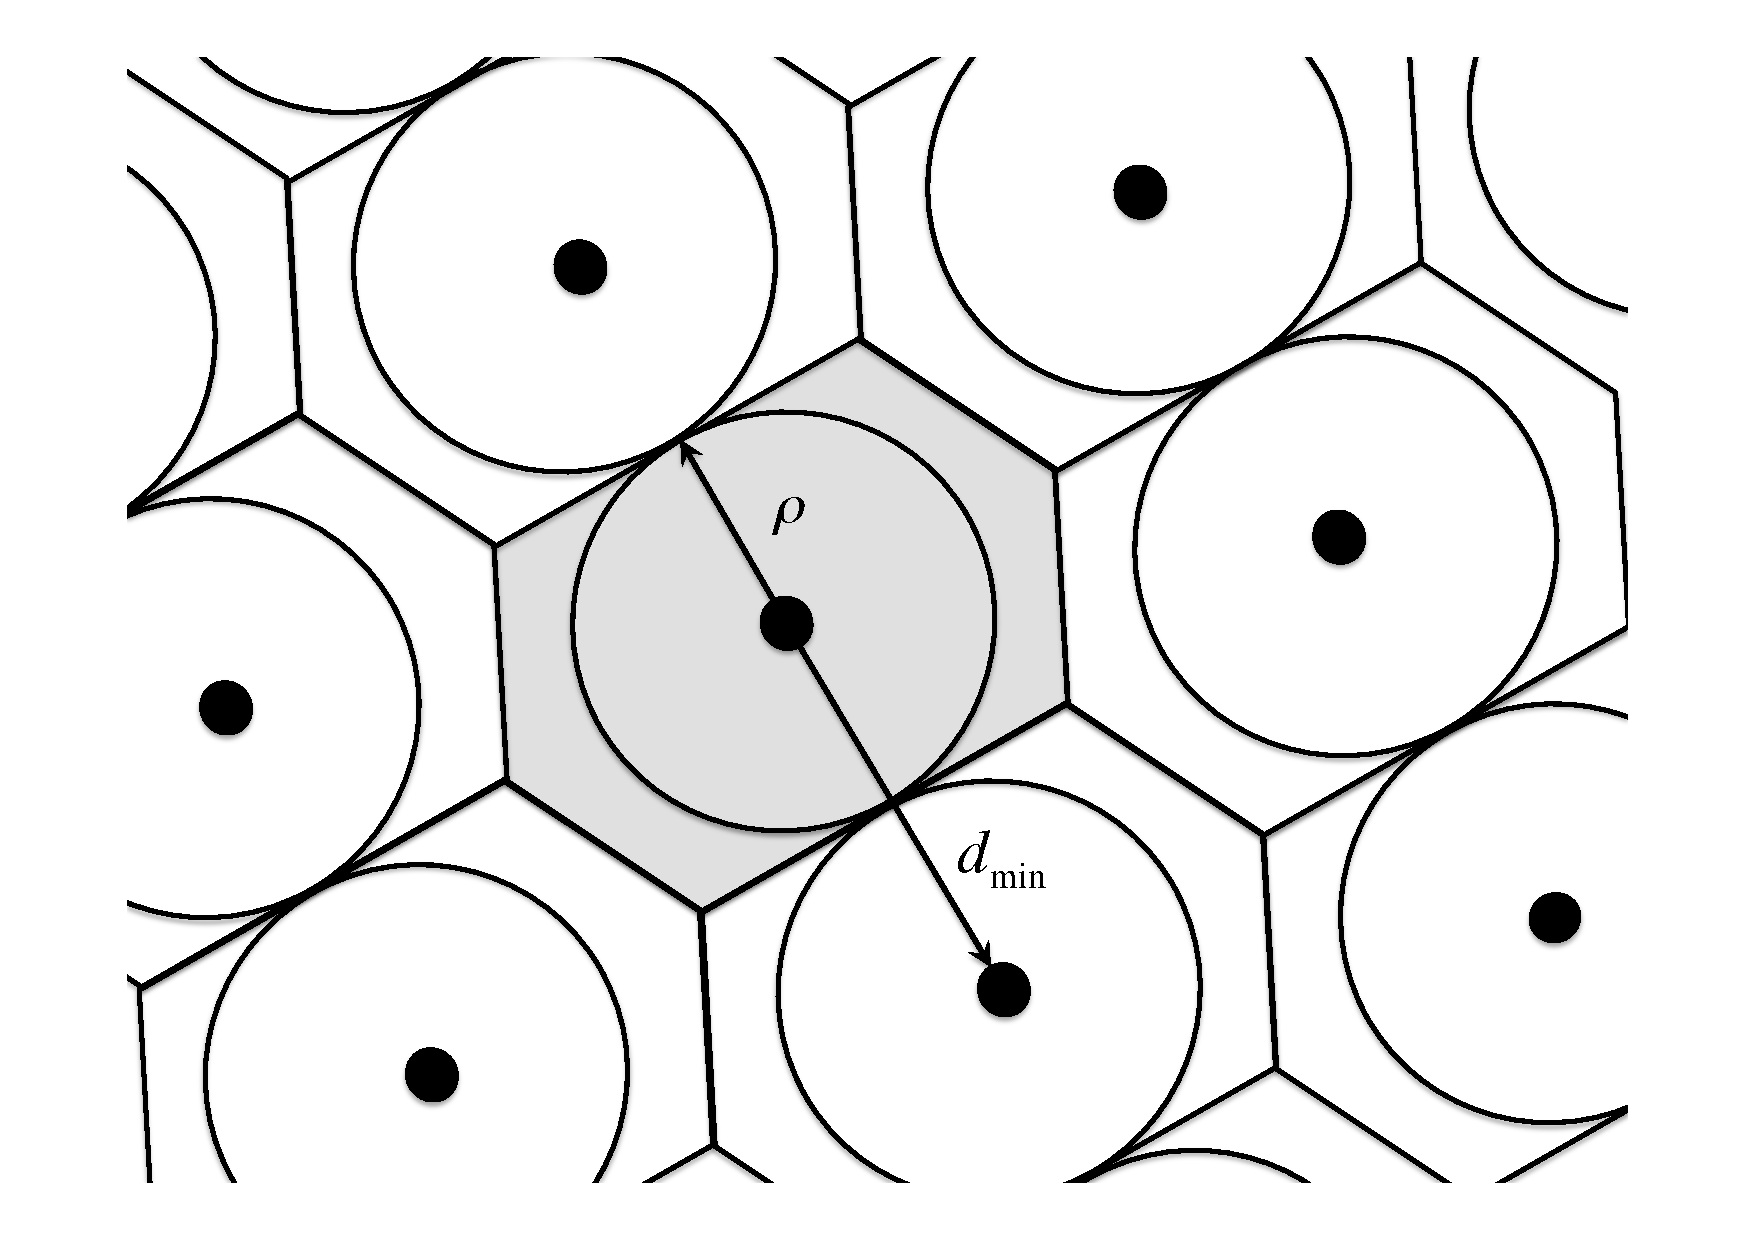
\includegraphics[scale=0.30]{figs/bound_dmin.pdf} 
%%\caption{The length of a short vector $\dmin$ and inradius $\rho = \dmin/2$ of the 2-dimensional lattice. This lattice has two short vectors. The shaded region shows the Voronoi cell of the lattice. The circles exhibit a sphere packing.}
%\includegraphics{figs/latticefigures-1.mps}
%\caption{The inradius $\rho = \dmin/2$ of the 2-dimensional lattice with basis $\bbf_1 = [3,0.72]^\prime, \bbf_2 = [0.6,3.6]^\prime$. The dots are the lattice points.  The origin $\zerobf$ is the lattice point in the center of the figure.  This lattice has two short vectors.  The shaded region shows the Voronoi cell of the lattice.  The solid circles exhibit a sphere packing.  The dashed circle has area (2-volume) equal to that of the Voronoi cell. The sphere with volume equal to the Voronoi cell is used in the upper bound~\ref{upperBoundUsingSphere}.}
%\label{fig:bound_dmin}
%\end{center}  
%\end{figure} 




%*********************************************************************************************************************************************************************************
\section{Approximating range error} \label{sec:appr-error-range}
%*********************************************************************************************************************************************************************************
In Section~\ref{sec:optim-freq-range} we will describe a procedure for selecting favourable sets of wavelengths for the least squares range estimator.  To do so, we first require approximations for the error of the range estimator in terms of the wavelengths $\lambda_1,\dots,\lambda_N$.  We consider two approximations.  The first approximates the error in the case that the least squares estimator of the wrapping variables $\hat{\zetabf}$ is correct.  The second uses~\ref{upperBoundUsingSphere} to upper bound the probability that $\hat{\zetabf}$ is correct.   

Recall from~\Sec{ch4:sec:phase-and-range-relation} that when the wrapping variables are correct $\Qbf \hat{\zetabf} = \Qbf \zetabf$ or equivalently $\zetabf = \hat{\zetabf} + k P \wbf$ for some $k \in \ints$.  In this case, the least squares estimator of the range takes the form~\ref{ch4:eq:rhatlinreg},
\[
\hat{r} = \frac{(\ybf - \hat{\zetabf})^\prime\wbf}{\wbf^\prime\wbf} = \frac{(\ybf - \zetabf + kP\wbf)^\prime\wbf}{\|\wbf\|^2}.
\]
Substituting~\ref{ch5:eq:Yndefn_vecform} for $\ybf$ we find that
\[
\hat{r} = \frac{\epsilonbf^\prime \wbf}{\|\wbf\|^2} + r_0 + kP.
\]
Recall from Section~\ref{ch4:sec:phase-and-range-relation} that range estimates $\hat{r}$ and $\hat{r} + kP$ are considered equivalent for integers $k$.  For this reason the error of the least squares range estimator corresponds with the term $\epsilonbf^\prime \wbf/\|\wbf\|^2$.  Under our assumption that $\epsilon_1,\dots,\epsilon_N$ are i.i.d. and normally distributed with zero mean and variance $\sigma^2$ this error is normally distributed with zero mean and variance
\begin{equation}\label{eq:approxwhenwrappingiscorrect}
\var \frac{\epsilonbf^\prime \wbf}{\|\wbf\|^2} = \frac{\sigma^2}{\|\wbf\|^2} = \frac{\sigma^2}{\sum_{n=1}^N \lambda_n^{-2}}.
\end{equation} 
The variance decreases as $\sum_{n=1}^N \lambda_n^{-2}$ increases.  The variance~\ref{eq:approxwhenwrappingiscorrect} serves as an approximation of the mean square error of the least squares range estimator when the estimated wrapping variables $\hat{\zetabf}$ are correct.  The simulation results in Section~\ref{sec:sim-results} suggest this approximation to be very close.

We now approximate the probability that the wrapping variables are correct, that is, we approximate the probability that $\Qbf\hat{\zetabf} = \Qbf\zetabf$.  Our approximation is based upon the upper bound~\ref{upperBoundUsingSphere}. Recall that $\hat{\zetabf}$ minimises the quadratic form $\|\Qbf \ybf - \Qbf \zbf\|^2$ over $\zbf \in \ints^N$.  It follows that $\Qbf \hat{\zetabf}$ is a closest point in the lattice $\Lambda^* = \{\Qbf \zbf \mid \zbf \in \ints^N \}$ to the point $\Qbf \ybf$.  Equivalently,
\[
\Qbf \ybf - \Qbf \hat{\zetabf} \in \vor\Lambda^*
\]
from the definition of the Voronoi cell.  Using~\ref{ch5:eq:Yndefn_vecform},
\[
\Qbf \ybf - \Qbf \hat{\zetabf} = \Qbf (r_0 \wbf + \epsilonbf + \zetabf) - \Qbf \hat{\zetabf} = \Qbf \epsilonbf - \Qbf(\hat{\zetabf} - \zetabf)
\]
and so
\[
\Qbf \epsilonbf - \Qbf(\hat{\zetabf} - \zetabf) \in \vor\Lambda^*.
\]
We see that $\Qbf(\zetabf - \hat{\zetabf})$ is a closest lattice point to the projection of the noise variables $\Qbf \epsilonbf$.  If $\Qbf \epsilonbf$ lies in the interior of the $\vor\Lambda^*$ then the unique closest lattice point is the origin $\zerobf$, that is, $\Qbf(\zetabf - \hat{\zetabf}) = \zerobf$ or equivalently $\Qbf\zetabf = \Qbf\hat{\zetabf}$.  We have found that the least square estimator $\hat{\zetabf}$ of the unwrapping variables is correct if the projection $\Qbf\epsilonbf$ of the noise variables lies within the interior of the Voronoi cell.  The estimator $\hat{\zetabf}$ can similarly be shown to be incorrect if $\Qbf\epsilonbf \notin \vor\Lambda^*$.  Because the boundary of the Voronoi cell has zero $n$-volume, it follows that the probability that unwrapping variables are correct is the same as the probability that $\Qbf\epsilonbf$ lies in $\vor\Lambda^*$

A further simplification can be made.  The $N-1$ dimensional lattice $\Lambda^*$ lies in the subspace orthogonal to $\wbf$ and so $\vor\Lambda^*$ is unbounded in the direction of $\wbf$.  Specifically, $\Qbf\epsilonbf \in \vor\Lambda^*$ if and only if $\Qbf \epsilonbf + s\wbf \in \vor\Lambda^*$ for all $s \in \reals$.  Because $\epsilonbf = \Qbf \epsilonbf + s \wbf$ for some $s$, it follows that $\Qbf \epsilonbf \in \vor\Lambda^*$ if and only if $\Qbf \epsilonbf + s\wbf = \epsilonbf \in \vor\Lambda^*$, that is,
\[
\Qbf \epsilonbf \in \vor\Lambda^* \Leftrightarrow \epsilonbf \in \vor\Lambda^*.
\]
Thus, the probability that the unwrapping variables are correct is the same as the probability that the noise $\epsilonbf$ lies in $\vor\Lambda^*$, that is, the same as the probability $P(\Lambda^*, \sigma^2)$ from~\ref{eq:probcorrectexact}.  We approximate this probability by the upper bound~\ref{upperBoundUsingSphere},
\begin{equation}\label{eq:upperboundcorrectwrapping}
P(\Lambda^*, \sigma^2) \leq F_{N-1}\left(\frac{\Gamma\big( \tfrac{N}{2} + \tfrac{1}{2} \big)^{2/(N-1)}}{\|\vbf\|^{2/(N-1)}\sigma^2 \pi}\right)
\end{equation}
where we have used the simple expression $\det\Lambda^* = \|\vbf\|^{-1}$ derived from Corollary~\ref{cor:intlatticedim1}.  This bound depends upon the wavelengths $\lambda_1,\dots,\lambda_N$ only through the term
\[
\|\vbf\|^2 = \|P\wbf\|^2 = P^2 \sum_{n=1}^N \lambda_n^{-2} = \lcm^2(\lambda_1,\dots,\lambda_N) \sum_{n=1}^N \lambda_n^{-2}.
\]
The bound increases as this term decreases.

This bound~\ref{eq:upperboundcorrectwrapping} for the probability of correct unwrapping is simpler than similar bounds in the literature that involve computing the determinant $\det\Lambda^* = \sqrt{\det \Bbf^\prime \Bbf}$ directly~\cite{Hassibi_GPS_1998,Li_distance_est_wrapped_phase}.  The simplicity of our bound is made possible by Corollary~\ref{cor:intlatticedim1} leading to the simple expression $\det\Lambda^* = \|\vbf\|^{-1}$.  This simplicity enables the wavelength selection procedure we describe in the next section.

% Substituting~\ref{eq:Yndefn} into $LS$ we obtain
% \[
% LS(r) = \sum_{n=1}^N \fracpart{\frac{r_0-r}{\lambda_n} + \Phi_n}^2.
% \] 

% Put
% \[
% z_{0n} = \round{Y_n - r_0 / \lambda_n}, \qquad n = 1,\dots,N
% \]
% and define the vector $\zbf_0 = (z_{01},\dots,z_{0N})$.  If it happens that $\hat{\zbf} = \zbf_0$ then, from~\ref{eq:leastsquaresrangehatz}, the least squares range estimator becomes
% \[
% \hat{r} = P\left( \frac{(\ybf - \zbf_0)^\prime\vbf}{\vbf^\prime\vbf} - \floor{\frac{(\ybf - \zbf_0)^\prime\vbf}{\vbf^\prime\vbf}}\right)
% \]

%*********************************************************************************************************************************************************************************
\section{Selecting wavelengths for range estimation}\label{sec:optim-freq-range}
%*********************************************************************************************************************************************************************************
In the previous section two approximations,~\ref{eq:approxwhenwrappingiscorrect} and~\ref{eq:upperboundcorrectwrapping}, related to range error were developed.  The first approximation~\ref{eq:approxwhenwrappingiscorrect} describes the variance of the range error when the wrapping variables are correct.  To decrease this variance we should choose wavelengths such that 
\[
\frac{\sigma^2}{\sum_{n=1}^N \lambda_n^{-2}}
\]
is small.  The second approximation~\ref{eq:upperboundcorrectwrapping} upper bounds the probability that the wrapping variables are correct.  To increase this bound we should choose wavelengths such that
\[
P^2 \sum_{n=1}^N \lambda_n^{-2} = \lcm^2(\lambda_1,\dots,\lambda_N) \sum_{n=1}^N \lambda_n^{-2}
\]
is small.  

\newcommand{\lambdamin}{\lambda_{\text{min}}}
\newcommand{\lambdamax}{\lambda_{\text{max}}}
\newcommand{\rmax}{r_{\text{max}}}

These are two competing objectives.  To have both small estimator variance while simultaneously allowing large probability of correct unwrapping we propose to choose wavelengths that minimise an objective function of the form
\begin{equation}\label{eq:Qobjectivefunction}
L(\lambda_1,\dots,\lambda_N) = P^2 \sum_{n=1}^N \lambda_n^{-2} + \frac{ \gamma}{\sum_{n=1}^N \lambda_n^{-2}}
\end{equation}
where $\gamma > 0$ weights the importance of the individual objectives and is free to be chosen. The weight $\gamma$ can be chosen to incorporate $\sigma^2$ if it is known.  We have found that choosing
\[
\gamma = \frac{N^2 \rmax^2}{\lambdamax^{2}\lambdamin^{2}}
\]
works well empirically.  The quantities $\rmax$, $\lambdamin$, and $\lambdamax$ will be introduced shortly.  This choice for $\gamma$ is used in the experiments performed in Section~\ref{sec:sim-results} and has the convenient property of being independent of the noise variance $\sigma^2$.  The choice is approximately the ratio of the minimum value of the two individual objectives. The motivation behind this being to approximately balance the importance given to both objectives. 

We incorporate into this optimisation problem three practical constraints.  First, we suppose that the wavelengths are all contained in an interval $[\lambdamin,\lambdamax]$.  In practice the minimum and maximum allowable wavelengths $\lambdamin$ and $\lambdamax$ might be dictated by hardware constraints, such as antennae size, or properties of the medium through which the signal propagates.  The second constraint is upon the maximum identifiable range.  We suppose that the system must be capable of unambiguously estimating range on an interval of some prespecified length $\rmax$, that is, $P \geq \rmax$.  For example $\rmax$ maybe a few meters for indoor applications, a few tens of meters for outdoor electronic surveying, and a few thousand kilometers for global positioning via satellite.  Finally, we assume that one of the wavelengths, say $\lambda_1$, is fixed and known.  We assume that $\lambda_1 = \lambdamax$ in what follows.  This constraint simplifies the optimisation problem and, since $\lambdamax$ is free to be selected, results in only minor loss of generality.  

Our optimisation problem is now to find wavelengths $\lambda_2,\dots,\lambda_{N}$ that minimise
\[
L_1(\lambda_2,\dots,\lambda_{N}) = L(\lambdamax,\lambda_2,\dots,\lambda_{N})
\]
subject to constraints
\begin{align}
&\lambdamin \leq \lambda_n \leq \lambdamax \qquad n = 2,\dots,{N} \label{eq:bandwidthcontraint} \\
&P = \lcm(\lambdamax,\lambda_2,\dots,\lambda_{N}) \geq \rmax. \label{eq:rangecontraint} 
\end{align}
These are referred to as the \emph{bandwidth constraint} and the \emph{range constraint} respectively.  The least common multiple $P = \lcm(\lambdamax,\lambda_2,\dots,\lambda_{N})$ depends upon the wavelengths in a non trivial way.  This optimisation problem is multivariate, nonlinear, and nonconvex with nonconvex constraints.  It is not immediately obvious how a solution is to be found.  We will show how this problem can be transformed into an equivalent problem involving $2(N-1)$ integer parameters.  This equivalent problem can be solved by a depth first search.

%First assume that the wavelengths are in decending order, that is, $\lambda_1 \geq \lambda_2 \geq \dots \geq \lambda_N$.  This assumption is without loss of generality because the objective function $L$ and the constraints are unchanged by permutation of $\lambda_1,\dots,\lambda_N$.  Under this assumption the range constraint can be refined to
% \begin{equation}
% \lambdamax \geq \lambda_{n-1} \geq \lambda_n \geq \lambda_{n+1} \geq \lambdamin \qquad n = 2,\dots,N-1. \label{eq:refinedbandwidthconstraint}
% \end{equation}
A solution of the minimisation problem is such that the wavelengths $\lambda_1 = \lambdamax$ and $\lambda_2, \dots, \lambda_{N-1}$ are rationally related, that is, $\lambda_n/\lambda_m$ is rational for all $n,m$.  Otherwise, $P = \lcm(\lambdamax,\lambda_2,\dots,\lambda_{N}) = \infty$ and $L_1$ will not be minimised. Thus, there exist positive integers $p_2,\dots,p_{N}$ and $q_2,\dots,q_{N}$ such that $\gcd(p_n,q_n) = 1$ and
\begin{equation}\label{eq:lambda-as-p-q}
\lambda_{n} = \frac{p_n}{q_n}\lambda_1 = \frac{p_n}{q_n}\lambdamax \qquad n = 2,\dots,N.
\end{equation}
%The case when $n = 1$ above asserts that $p_1 = q_1 = 1$.  %Also, because $\lambda_1 \geq \lambda_n$ we have $q_n \geq p_n$.  
Now,
\begin{equation}\label{eq:P-as-p-q} 
P = \lcm\left(\lambdamax, \frac{p_2}{q_2}\lambdamax, \dots, \frac{p_N}{q_N}\lambdamax \right) = \lambdamax Q
\end{equation}
where
\[
Q = \lcm\left(1,  \frac{p_2}{q_2}, \dots, \frac{p_N}{q_N} \right).
\]
A simpler expression for $Q$ can be obtained.  %First observe that $\lcm(d,a/b) = \lcm(d,a)$ is an integer if $d$ is an integer and $a$ and $b$ are relatively prime integers.  
Let $\ell_1,\dots,\ell_N$ satisfy
\[
\ell_1 = 1, \qquad \ell_{n} = \lcm\left( \ell_{n-1}, \frac{p_n}{q_n} \right) \qquad n = 2,\dots,N
\]
and observe that $Q = \ell_N$.  Because $\ell_1$ is an integer and $p_2$ and $q_2$ are relatively prime $\ell_2 = \lcm(\ell_1,p_2/q_2) = \lcm(1,p_2)$ is an integer.  Similarly,
\[
\ell_3 = \lcm\left(\ell_2,\frac{p_3}{q_3}\right) = \lcm(\ell_2,p_3) = \lcm(1,p_2,p_3) 
\]
is an integer and, by induction,
\[
\ell_N = \lcm\left(\ell_{N-1},\frac{p_N}{q_N}\right) = \lcm(1,p_2,\dots,p_N).
\]
Now $Q = \ell_N = \lcm(p_2,\dots,p_N)$.  Observe that $Q$ does not depend on the denominators $q_2,\dots,q_N$.  It is convenient to introduce vectors $\pbf = (p_2,\dots,p_N)$ and $\qbf = (q_2,\dots,q_N)$ and write $Q(\pbf)$ to highlight the dependence of $Q$ on $p_2,\dots,p_N$.

From the range constraint~\ref{eq:rangecontraint} and \ref{eq:P-as-p-q},
\begin{equation}\label{eq:reecondedrangeconst}
Q(\pbf) = \lcm(p_2, \dots, p_N) = \frac{P}{\lambdamax} \geq \frac{\rmax}{\lambdamax}
\end{equation}
and from the bandwidth constraint~\ref{eq:bandwidthcontraint} and \ref{eq:lambda-as-p-q},
\begin{equation}\label{eq:reecondedbrandwidthconst}
\frac{\lambdamin}{\lambdamax} \leq \frac{p_{n}}{q_{n}} \leq 1 \qquad n = 2,\dots,N.
\end{equation}
Define the objective function
\begin{align}
L_2(\pbf,\qbf) &= L_1\big(\tfrac{p_2}{q_2}\lambdamax, \dots, \tfrac{p_N}{q_N}\lambdamax\big) \nonumber \\
&= Q^2(\pbf) D(\pbf,\qbf) + \frac{ \gamma \lambdamax^2}{D(\pbf,\qbf)}.  \label{eq:objectvefunctionL1}
\end{align}
where 
\begin{equation}\label{eq:D-p-q}
D(\pbf,\qbf) = 1 + \sum_{n=2}^N \frac{q_n^2}{p_n^2}.
\end{equation}
Our optimisation problem can now be re-encoded into that of finding integers vectors 
\[
\hat{\pbf} = (\hat{p}_2,\dots,\hat{p}_N), \qquad \hat{\qbf} = (\hat{q}_2,\dots,\hat{q}_N)
\]
that minimise $L_2$ subject to constraints~\ref{eq:reecondedrangeconst}~and~\ref{eq:reecondedbrandwidthconst}.  Given these minimisers, the wavelengths
\[ 
\hat{\lambda}_n = \frac{\hat{p}_n}{\hat{q}_n} \lambdamax \qquad n = 2,\dots,N
\]
are a solution of the original optimisation problem, that is, these wavelengths minimise $L_1$ subject to the bandwidth and range constraints~\ref{eq:bandwidthcontraint}~and~\ref{eq:rangecontraint}.  We now describe an algorithm to find minimisers $\hat{\pbf}$ and $\hat{\qbf}$.

% For fixed $\lambda_1$ we will be able to minimise $L_1$ with respect to the integers $p_2,\dots,p_N, q_2,\dots,q_N$ by a depth first search.  That is, we will be able to compute the function
% \[
% L_2(\lambda_1) = \min_{p,q \in \ints^{N-1}} L_1(\lambda_1,p,q)
% \]
% where the minimisation is subject to constraints~\ref{eq:reecondedrangeconst}~and~\ref{eq:reecondedbrandwidthconst}.  Given $L_2$, the optimised wavelength $\hat{\lambda}_1$ can be approximated by minimising $L_2$ over a grid 
% \[
% \lambdamax, \;\;  \lambdamax - \delta, \;\; \lambdamax - 2\delta, \;\; \cdots \;\; \lambdamax - \floor{\tfrac{\lambdamax - \lambdamin}{\delta}} \delta
% \]
% uniformly spaced on the interval $[\lambdamin, \lambdamax]$.  The approximation can be made as close as desired by chooseing $\delta$ small.  It remains to describe a method of minimising $L_1$ with respect to the integers $p_2,\dots,p_N, q_2,\dots,q_N$ for fixed $\lambda_1$, that is, a method for computing the function $L_2$.

We first discover some bounds that the minimisers $\hat{p}_n,\hat{q}_n$ must satisfy.  From~\ref{eq:reecondedbrandwidthconst} and \ref{eq:D-p-q},
\begin{equation}\label{eq:Dineq}
N \leq D(\hat{\pbf},\hat{\qbf})  \leq  1 + \frac{(N-1)\lambdamax^2}{\lambdamin^2}.
\end{equation}
Also
\begin{equation}\label{eq:Qineq}
Q(\hat{\pbf}) = \lcm(\hat{p}_2,\dots,\hat{p}_N) \geq \hat{p}_n \qquad n = 2,\dots,N.
\end{equation}
Let $\widehat{L} = L_2(\hat{\pbf},\hat{\qbf})$ be the minimum value of $L_2$ (and also of $L_1$) and let $\widetilde{L}$ be a finite upper bound on $\widehat{L}$.  For example, it suffices to choose
\begin{equation}\label{eq:L-tilde}
\widetilde{L} = L_1\big(\tfrac{w}{w+1}\lambdamax,\dots,\tfrac{w}{w+1}\lambdamax\big)
\end{equation}
where $w$ is the smallest integer greater than or equal to both $\rmax/\lambdamax$ and $\lambdamin/(\lambdamax-\lambdamin)$.  With this choice $\tfrac{w}{w+1}\lambdamax \in [\lambdamin, \lambdamax]$ so that the bandwidth constraint is satisfied and
\begin{align*}
\lcm\big(\lambdamax,\tfrac{w}{w+1}\lambdamax,\dots,\tfrac{w}{w+1}\lambdamax\big) = \lambdamax w \geq r_{\text{min}}
\end{align*}
so that the range constraint is satisfied.  Now, 
\[
\widetilde{L} \geq \widehat{L} = Q(\hat{\pbf})^2D(\hat{\pbf},\hat{\qbf}) + \frac{ \gamma \lambdamax^2}{D(\hat{\pbf},\hat{\qbf})} 
\]
and using the inequalities~\ref{eq:Qineq} for $Q(\hat{\pbf})$ and~\ref{eq:Dineq} for $D(\hat{\pbf},\hat{\qbf})$ we find that,
\[
\widetilde{L} \geq \widehat{L} \geq \hat{p}_n^2 N + \gamma B \qquad \text{for all $n = 2,\dots,N$}
\]
where 
\[
B = \frac{\lambdamin^2 \lambdamax^2}{\lambdamin^2 + (N-1)\lambdamax^2}.
\]
Because $\hat{p}_n \geq 1$ is a positive integer we obtain the following lower and upper bounds
\begin{equation}\label{eq:pkbound}
1 \leq \hat{p}_n \leq \sqrt{\frac{\widetilde{L} - \gamma B}{N}} \qquad n = 2,\dots,N.
\end{equation}
Given $\hat{p}_n$ upper and lower bounds on $\hat{q}_n$ derive from the bandwidth constraint~\ref{eq:reecondedbrandwidthconst},
 \begin{equation}\label{eq:qkbound}
 \hat{p}_n \leq \hat{q}_n \leq \frac{\lambdamax}{\lambdamin} \hat{p}_n \qquad n = 2,\dots,N.
 \end{equation}
To find minimisers of $L_2$, it suffices to check only those integer vectors $\hat{\pbf}$ and $\hat{\qbf}$ with elements satisfying the above two inequalities \ref{eq:pkbound} and \ref{eq:qkbound}.  Because the number of integer vectors satisfying these inequalities are finite this procedure will terminate in finite time.  The number of candidate solutions that need to be checked can be reduced by incorporating the property $\gcd(\hat{p}_n, \hat{q}_n) = 1$ into the search.  The number of candidates is further reduced by noting that the objective function $L_1$ is unchanged by permutation of the wavelengths $\lambda_2,\dots,\lambda_N$.  Equivalently, $L_2(\pbf,\qbf)$ is unchanged if both arguments $\pbf$ and $\qbf$ undergo the same permutation.  For this reason it is sufficient to suppose that the elements of $\hat{\pbf}$ are in, say, ascending order, that is, $\hat{p}_2 \leq \hat{p}_3 \leq \cdots \leq \hat{p}_N$. 

Psuedocode describing the search procedure is given in Algorithm 1. The algorithm makes use of two functions $\operatorname{psearch}$ and $\operatorname{qsearch}$ that are called recursively.  The integer variables $N$, $p_2,\dots,p_N$, $q_2,\dots,q_N$, and the real variables $\widetilde{L}, \gamma, B$ are assumed to be globally accessible to both functions $\operatorname{psearch}$ and $\operatorname{qsearch}$.  The while loop on line~\ref{alg:psearch:whilepn} of $\operatorname{psearch}$ iterates over those $p_n$ satisfying~\ref{eq:pkbound}. The while loop on line~\ref{alg:qsearch:whileqn} of $\operatorname{qsearch}$ iterates over those $q_n$ satisfying~\ref{eq:qkbound}.  The condition on line~\ref{alg:qsearch:ifgcd} of $\operatorname{qsearch}$ ensures that only those relatively prime $p_n, q_n$ are included in the search. Lines~\ref{alg:updateif} to~\ref{alg:updatewavelengths} update the minimum found value of the objective function $\tilde{L}$ and the corresponding wavelengths whenever a new minimiser of the objective function $L_2$ is found.

This depth first search becomes computationally expensive if the number of wavelengths is not small or the minimum range $\rmax$ is large when compared with the maximum wavelength $\lambdamax$.  For this reason we now suggest some methods that accelerate the search at the expense of not necessarily guaranteeing that the true minimisers of $L$ are found.  The first method simply terminates the search after a specified amount of time and takes the best wavelengths found to that point.  This approach is simple, but can be highly effective because the minimisers of $L$ are regularly found well before the search completes.

The second method places a more restrictive upper bound on $\hat{p}_2,\dots,\hat{p}_N$.  The upper bound is motivated by physical constraints regularly occurring in practice that limit the accuracy to which a signal of a given wavelength can be generated~\cite[Sec.~5.B]{Falaggis_algebraic_solution_2014}.   Rather than the upper bound from~\ref{eq:pkbound} a smaller fixed constant, say $\kappa$, is chosen and those $p_n$ satisfying $1 \leq \hat{p}_n \leq \kappa$ are searched.  The condition on Line~\ref{alg:psearch:whilepn} of $\operatorname{psearch}$ is correspondingly modified to $p_n \leq \kappa$.   From ~\ref{eq:qkbound} we see that the new bound on $\hat{p}_n$ places a new bound on $\hat{q}_n$,
\[
\hat{q}_n \leq \frac{\lambdamax}{\lambdamin} \hat{p}_n \leq \frac{\lambdamax}{\lambdamin} \kappa
\]
Recall that the wavelengths take the form $\hat{\lambda}_n = \hat{p}_n \lambdamax/\hat{q}_n$ and so this new bound limits the resolution of the wavelengths searched by the optimiser.  Specifically, the wavelengths are restricted to the form $\lambdamax p/q$ where $p \leq q$ and $q$ is smaller than $\kappa\lambdamax/\lambdamin$.

\begin{algorithm} \label{alg:main}
\SetAlCapFnt{\small} 
\SetAlTitleFnt{}
\DontPrintSemicolon
\KwIn{$N, \rmax, \lambdamin, \lambdamax, \gamma$}
$d = \ceil{\max\big(\frac{\rmax}{\lambdamax}, \frac{\lambdamin}{\lambdamax-\lambdamin}\big)}$ \;
$(\hat{\lambda}_2, \dots, \hat{\lambda}_N) = \big(\tfrac{w}{w+1}\lambdamax,\dots,\tfrac{w}{w+1}\lambdamax\big)$ \;
$\widetilde{L} = L_1\big(\hat{\lambda}_2, \dots, \hat{\lambda}_N)$ \;
$B = \frac{\gamma \lambdamin^2 \lambdamax^2}{\lambdamin^2 + (N-1)\lambdamax^2}$\;
$p_2 = 1$ \;
$\operatorname{psearch}(2)$ \;
\KwRet{$(\lambdamax , \hat{\lambda}_2, \dots, \hat{\lambda}_N)$}  
\caption{Computes wavelengths optimised for the least squares range estimator.}
\end{algorithm}

\begin{function} \label{alg:psearch}
\SetAlCapFnt{\small}
\SetAlTitleFnt{}
\DontPrintSemicolon
\KwIn{$n \in \{2,\dots,N \}$}
\While{$p_{n}^2 \leq (\widetilde{L} - \gamma B)/N$ \nllabel{alg:psearch:whilepn} }{
$q_n = p_n$ \;
$\operatorname{qsearch}(n)$ \;
$p_n = p_n+1$ 
}
\caption{psearch($n$)}
\end{function}

\begin{function} \label{alg:qsearch}
\SetAlCapFnt{\small}
\SetAlTitleFnt{}
\DontPrintSemicolon
\KwIn{$n \in \{2,\dots,N \}$}
\While{ $q_n \leq p_n \lambdamax/\lambdamin$ \nllabel{alg:qsearch:whileqn} } {
\If{ $\gcd(p_n,q_n) = 1$ \nllabel{alg:qsearch:ifgcd} } {
\If{ $n < N$ } {
$p_{n+1} = p_n$ \;
$\operatorname{psearch}(n+1)$ \;
}
\ElseIf{$L_2(\pbf,\qbf) \leq \widetilde{L}$ \emph{and} $\lcm(\pbf) \geq \tfrac{\rmax}{\lambdamax}$ \nllabel{alg:updateif} } {
$\widetilde{L} = L_2(\pbf,\qbf)$ \;
$\hat{\lambda}_n = \lambdamax p_n/q_n \;\; n = 2,\dots,N$ \nllabel{alg:updatewavelengths} \;
}
}
$q_n = q_n + 1 $
}
\caption{qsearch($n$)}
\end{function}

In practice we cannot generate sinusoidal signals with arbitrarily precise wavelengths.  For example, optical interferometric experiments are limited by uncertainties in the refractive index of the medium through which the signal propagates~\cite[Sec.~5.B]{Falaggis_algebraic_solution_2014}.  Audio and radio frequency devices are limited by the stability of oscillators used to generate signals.  For these reasons, restricting the wavelength optimisation to a finite resolution is likely to be of little practical consequence.  It might even be necessary for some applications.  In practice, one might select $\kappa$ so that $\kappa\lambdamax/\lambdamin$ is related to the precision with which a sinusoidal signal can be generated. 


\section{Numerical Results}\label{sec:sim-results}
We present the results of Monte-Carlo simulations with the least squares range estimator, the excess fractions estimator~\cite{Falaggis_excess_fractions_2011},  the algebraic method of Falaggis~et~al.~\cite{Falaggis_algebraic_solution_2014}, the beat wavelength method of~Towers~et~al.~\cite{Towers_frequency_selection_interferometry_2003}, and range estimators based on the single-stage and multi-stage CRT algorithms of Xiao~et~al.~\cite{Xiao_multistage_crt_2014}. %the least squares range estimator, the range estimator based on the method of excess fractions~\cite{Falaggis_excess_fractions_2011} and the range estimator based on the single stage and multi-stage CRT algorithms of Xiao~et.~al.~\cite{Xiao_multistage_crt_2014}. 
In each simulation the phase noise variables $\Phi_1,\dots,\Phi_N$ are wrapped normally distributed, that is, $\Phi_n = \fracpart{\epsilon_n}$ where $\epsilon_1,\dots,\epsilon_N$ are independent and normally distributed with zero mean and variance $\sigma^2$.  The number of Monte-Carlo trials used for each value of $\sigma^2$ is $10^5$. 

\fig{fig:leastsquares_EF_CRT_N3} shows the sample mean square error of these estimators for $N=3$ wavelengths. In each simulation the true range is $r_0 = 6\pi$ and we consider three different sets of wavelengths
\[
A = \{ 2 , 3, 5\},
\]
\[ 
B = \{  \tfrac{30}{13}, \tfrac{15}{4}, 5\},
\]
\[
C = \{  2,   \tfrac{2142857142857143}{10^{12}},   \tfrac{2696140478029631}{10^{15}} \}.
\]
The wavelengths from all the sets are contained in the interval $[2, 5]$ and the identifiable range is $\lcm(A)=\lcm(B)=30$. The wavelengths $A$ are used in the simulations of Li et. al.~\cite{Li_distance_est_wrapped_phase} and $B$ are optimised wavelengths given by Algorithm 1. Wavelengths $C$ are obtained using optimal wavelengths selection for the beat wavelength method of~Towers~et~al.~\cite{Towers_frequency_selection_interferometry_2003} to measure the same distance of $\rmax=30$. The maximum range of the beat wavelength method is equal to the largest synthetic/beat wavelength generated. When the noise variance is small the probability that the wrapping variables are correct is large and so we expect the mean square error of the least squares estimator to be similar to~\ref{eq:approxwhenwrappingiscorrect}.  This predicted mean square error is shown by the solid line for wavelengths $A$ and by the dashed line for wavelengths $B$.  Observed from~\fig{fig:leastsquares_EF_CRT_N3} that these predictions accurately model the behaviour of the least squares estimator when $\sigma^2$ is small.  

Wavelengths $A$ result in slightly reduced sample mean square error compared with $B$ when $\sigma^2$ is small.  As $\sigma^2$ increases the sample mean square error exhibits a `threshold' effect and increases suddenly. The threshold occurs at $\sigma^2 \approx 5 \times 10^{-4}$ with wavelengths $A$ and $\sigma^2 \approx 9 \times 10^{-4}$ with wavelength $B$ for the least squares estimator. Wavelengths $B$ are more accurate than $A$ when $\sigma^2$ is greater than approximately $5 \times 10^{-4}$. The threshold for the CRT and excess fractions based range estimators occurs at approximately the same value of $\sigma^2$ with wavelengths $A$. The CRT estimator performs poorly with wavelengths $B$. The threshold for the excess fractions estimator is similar to that of the least squares estimator with wavelength $B$.  However, the mean square error of the excess fraction estimator is larger than that of the least squares estimator when the noise variance is small. The beat wavelength estimator with wavelengths $C$ performs poorly compared with the least squares and the excess fractions estimators with wavelengths $A$ and $B$. The threshold for the beat wavelength method with wavelengths $C$ occurs at $\sigma^2 \approx 3 \times 10^{-4}$. 

\begin{figure}[t]
  \centering 
  \begin{tikzpicture}
    \selectcolormodel{gray}
    \begin{axis}[font=\footnotesize,xmode=log,ymode=log,height=10cm,width=12cm,ylabel={MSE},ylabel style={at={(-0.1,0.5)}},xlabel style={at={(0.53,-0.05)}}, legend style={draw=none, fill=none, at={(1,1)},xmin=4e-5,xmax=7e-2, legend pos=south east, cells={anchor=west}, inner xsep = 1pt, inner ysep = 1pt, nodes = {inner sep=0.05pt, text depth = 0.05cm}},xlabel={$\sigma^2$}]
	\addplot[mark=*,only marks,mark options={scale= 0.7}] table {chapters/ch5/data/LeastSquaresA};
	\addplot[mark=o,only marks,mark options={fill=black , scale=  1}] table {chapters/ch5/data/LeastSquaresB};
	\addplot[mark=diamond,only marks,mark options={fill=black , scale=  1}]table {chapters/ch5/data/CRTA};
	\addplot[mark=square, only marks,mark options={fill=black , scale=  1}]table {chapters/ch5/data/CRTB};
	\addplot[densely dashdotted]table {chapters/ch5/data/ExcessFractionsA};
	\addplot[densely dotted]table {chapters/ch5/data/ExcessFractionsB};
	\addplot[mark=square,mark options={solid}]table {chapters/ch5/data/TowersC};
        \addplot[solid ,domain=4e-5:7e-2] {x/( 1/2/2 + 1/3/3+ 1/5/5 )};
	\addplot[loosely dashed ,domain=4e-5:7e-2] {x/( 13/30*13/30 + 4/15*4/15 + 1/5*1/5 )};
        %\addplot[mark=o,only marks,mark options={scale= 0.5}] table {chapters/ch5/data/LeastSquaresD};
        
	\legend{Least squares $A$, Least squares $B$, CRT $A$, CRT $B$, EF $A$, EF $B$, Beat wavelength $C$, MSE $A$ using \ref{eq:approxwhenwrappingiscorrect}, MSE $B$ using \ref{eq:approxwhenwrappingiscorrect},}
   \end{axis}  
  \end{tikzpicture}    
 \caption{Sample mean square error of the least squares range estimator, the excess fraction based range estimator~\cite{Falaggis_excess_fractions_2011}, the beat wavelength method~\cite{Towers_frequency_selection_interferometry_2003}, and the range estimator based on the single stage and multi-stage CRT algorithms of Xiao~et.~al.~\cite{Xiao_multistage_crt_2014} with $N=3$ wavelenths.}
  \label{fig:leastsquares_EF_CRT_N3}   
\end{figure} 

\fig{fig:leastsquares_EF_CRT_N4_1} displays the simulations results when there are $N=4$ wavelengths from the sets
\[
D = \{ \tfrac{101039}{66}, \tfrac{1076285}{682}, \tfrac{198036440}{125389}, \tfrac{17572}{11} \},
\]
\[
%B  = \{  1528,   \tfrac{26309}{17}, \tfrac{20404}{13}, \tfrac{17572}{11}  \}.
E  = \{  1528,   \tfrac{3868970284693}{25\times 10^8}, \tfrac{156953786407767}{10^{11}}, \tfrac{17572}{11}  \}.
\]
\[
F = \{1528,   \tfrac{1528064857863967}{10^{12}},   \tfrac{1529861512776706}{10^{12}},   \tfrac{1583226826910749}{10^{12}}\}
\]
%\[
%C = \{1539, 1540, 1595, 1596 \}
%\]
%\[
%D = \{1528, 1528, 1543, 1597   \}
%\]
\normalsize 

The wavelengths from all the sets are contained in the interval $[1528 , \tfrac{17572}{11}]$.  Wavelengths $E$ are those selected for the excess fractions estimator using the procedure described in~\cite{Falaggis_excess_fractions_2012}.  These wavelengths are measured in nanometers in~\cite{Falaggis_excess_fractions_2012}.  The least common multiple of $E$ is greater than $2 \times 10^{22}$ meters.  However, the maximum range of the excess fractions estimator is not the least common multiple, but is instead what is called the \emph{unambiguous measurement range} (UMR)~\cite{Falaggis_excess_fractions_2012} and is $1.8\times10^7\si{\nano\meter} = \SI{0.018}{\meter}$ in this case. Wavelengths $F$ are optimal wavelengths for the beat wavelength method and are obtained using optimal wavelength selection method of~Towers~et~al~\cite{Towers_frequency_selection_interferometry_2003} to measure the same distance of $1.8\times10^7\si{\nano\meter} = \SI{0.018}{\meter}$. Wavelengths $D$ are optimised for the least squares estimator using Algorithm 1 with $\rmax = 1.8\times 10^7$ equal to the UMR.  To speed up the search we put $\kappa = 1000$ as described in Section~\ref{sec:optim-freq-range}.  The identifiable range with wavelengths $D$ is 
\[
\lcm(D) =  198036440/11 \approx 18003312 > 1.8\times 10^7.
\]  

In each simulation the true range $r_0 = 4000000\pi \approx 0.7 \rmax$.  It can be observed from this figure that the single and multi-stage CRT estimators~\cite{Xiao_multistage_crt_2014} and the algebraic method of Falaggis~et~al.~\cite{Falaggis_algebraic_solution_2014} perform very poorly when compared with the beat wavelength, the excess fractions~\cite{Falaggis_excess_fractions_2011} and the least squares estimator. 
%When $\sigma^2$ is less than $ \approx 5\times 10^{-11}$ the single and multi-stage CRT estimators perform similar to the least squares estimator. When $\sigma^2$ is less than $ \approx 9\times 10^{-8}$ the modified excess fractions based estimator performs slightly poor than the least squares estimator. 
When $\sigma^2$ is less than $ \approx 8\times10^{-6}$ the least squares estimator is slightly more accurate than the beat wavelength and the excess fractions estimator. %However, when $\sigma^2$ is greater than $ \approx 2\times 10^{-7}$ the least squares and the CRT estimators outperform the modified excess fractions based estimator.
%As $\sigma^2$ increases the sample mean square error exhibits a threshold' effect and increases suddenly.
%The threshold for the least squares estimator occurs at $ \approx 10^{-4.8}$ whereas the threshold for the single and multi-stage CRT, the modified excess fractions, and the excess fractions based estimators occur at $ \approx 4\times 10^{-11}$, $ \approx 8\times 10^{-8}$, and $ 10^{-5}$ respectively.
The thresholds for the beat wavelength, the excess fractions and the least squares estimators occur at approximately $7 \times 10^{-6}$, $10^{-5}$ and  $2 \times 10^{-5}$ respectively. The least squares estimator is the most accurate among the estimators. It can also be observed that \ref{eq:approxwhenwrappingiscorrect} provides a very good approximation for the MSE of the least squares estimator.


%The performance of the classical excess fractions based estimator is similar for the wavelengths $A$ and $B$ respectively. When the noise variance $\sigma^2$ is small the least squares estimator exhibits smaller mean square error with wavelengths $A$ as compared to that of excess fractions based range estimator with wavelengths $B$. As $\sigma^2$ increases the sample mean square error exhibits a �threshold� effect and increases suddenly. Single stage estimator with wavelengths $C$ performs poorly compared to the least squares and excess fractions range estimators with wavelengths $A$ and $B$ respectively. A large improvement is gained by use of the multi-stage CRT estimator by splitting the wavelengths from $C$ into two sets $\{ 1596, 1539 \}$ and $\{ 1595, 1540\}$. Simulations indicate that this is the best splitting of the wavelengths for the multi-stage CRT estimator in this case. Two stage CRT estimator performs similar to the least squares range estimator with wavelengths $A$ and slightly better than the excess fractions range estimator with wavelengths $B$ when the noise variance $\sigma^2$ is less than $ \approx 4\times 10^{-6}$. Least sqaures range estimator with wavelengths $D$ performs very poorly as compared to least squares, excess fractions and CRT estimators with wavelengths $A$, $B$ and $C$ respectively as indicated in the simulation results.

\begin{figure}[t]
  \centering 
  \begin{tikzpicture}
    \selectcolormodel{gray}
    \begin{axis}[font=\footnotesize,xmode=log,ymode=log,height=10cm,width=12cm,ylabel={MSE},ylabel style={at={(-0.1,0.5)}},xlabel style={at={(0.53,-0.05)}}, legend style={draw=none, fill=none, at={(1,1)}, legend pos=south east,cells={anchor=west}, inner xsep = 1pt, inner ysep = 1pt, nodes = {inner sep=0.05pt, text depth = 0.05cm}},xmin=1e-6,xmax=3e-4,ymin=1e-6,ymax=1e15,xlabel={$\sigma^2$}]
	\addplot[mark=o,only marks,mark options={scale= 1}] table {chapters/ch5/data/LeastSquaresD};
	\addplot[densely dashdotted] table {chapters/ch5/data/ExcessFractionsE};
	\addplot[dotted]table {chapters/ch5/data/ExcessFractionsAlgebraicE};
	\addplot[solid, mark=diamond,only marks,mark options={fill=black , scale=  1}]table {chapters/ch5/data/CRTD};
	\addplot[solid, mark=square,only marks,mark options={fill=black , scale=  1}]table {chapters/ch5/data/TwoStageCRTD};
	\addplot[mark=square,mark options={solid}]table {chapters/ch5/data/TowersF};
	\addplot[loosely dashed ,domain=1e-6:7e-2] {x/( 66/101039*66/101039 + 682/1076285*682/1076285 + 125389/198036440*125389/198036440 + 11/17572*11/17572 )};
        %\addplot[mark=o,only marks,mark options={scale= 0.5}] table {chapters/ch5/data/LeastSquaresD};
        
	\legend{Least squares D, EF method E, Algebraic method E,  1-stage CRT D, 2-stage CRT D, Beat wavelength F, MSE D using \ref{eq:approxwhenwrappingiscorrect} }
   \end{axis}  
  \end{tikzpicture}    
 \caption{Sample mean square error of the least squares range estimator, the excess fraction based range estimator~\cite{Falaggis_excess_fractions_2011}, the algebraic method of Falaggis~et~al.~\cite{Falaggis_algebraic_solution_2014}, the beat wavelength method~\cite{Towers_frequency_selection_interferometry_2003}, and the range estimator based on the single stage and multi-stage CRT algorithms of Xiao~et.~al.~\cite{Xiao_multistage_crt_2014} with $N=4$ wavelenths.}
  \label{fig:leastsquares_EF_CRT_N4_1}   
\end{figure} 

%\begin{figure}[t]
%  \centering 
%  \begin{tikzpicture}
%    \selectcolormodel{gray}
%    \begin{axis}[font=\footnotesize,xmode=log,ymode=log,height=10cm,width=12cm,ylabel={MSE},ylabel style={at={(-0.1,0.5)}},xlabel style={at={(0.53,-0.05)}}, legend style={draw=none, fill=none, at={(1,1)}, legend pos=south east,cells={anchor=west}, inner xsep = 1pt, inner ysep = 1pt, nodes = {inner sep=0.05pt, text depth = 0.05cm}},xmin=1e-6,xmax=3e-4,ymin=1e-6,ymax=1e15,xlabel={$\sigma^2$}]
%	\addplot[mark=o,only marks,mark options={scale= 1}] table {chapters/ch5/data/LeastSquaresC2};
%	\addplot[densely dashdotted] table {chapters/ch5/data/ExcessFractionsD2};
%	\addplot[dotted]table {chapters/ch5/data/ExcessFractionsAlgebraicD2};
%	\addplot[solid, mark=diamond,only marks,mark options={fill=black , scale=  1}]table {chapters/ch5/data/CRTC2};
%	\addplot[solid, mark=square,only marks,mark options={fill=black , scale=  1}]table {chapters/ch5/data/TwoStageCRTC2};
%	\addplot[loosely dashed ,domain=1e-6:7e-2] {x/( 66/101039*66/101039 + 682/1076285*682/1076285 + 125389/198036440*125389/198036440 + 11/17572*11/17572 )};
%        %\addplot[mark=o,only marks,mark options={scale= 0.5}] table {chapters/ch5/data/LeastSquaresD};
%        
%	\legend{Least squares C, EF method D, Algebraic method D, 1-stage CRT C, 2-stage CRT C, MSE C using \ref{eq:approxwhenwrappingiscorrect} }
%   \end{axis}  
%  \end{tikzpicture}    
% \caption{Sample mean square error of the least squares range estimator, the excess fraction based range estimator~\cite{Falaggis_excess_fractions_2011}, the algebraic method of Falaggis~et~al.~\cite{Falaggis_algebraic_solution_2014} and the range estimator based on the single stage and multi-stage CRT algorithms of Xiao~et.~al.~\cite{Xiao_multistage_crt_2014} with $N=4$ wavelenths.}
%  \label{fig:leastsquares_EF_CRT_N4_1}   
%\end{figure} 
%\begin{figure}[t]
%  \centering 
%  \begin{tikzpicture}
%    \selectcolormodel{gray}
%    \begin{axis}[font=\footnotesize,xmode=log,ymode=log,height=8cm,width=9cm,ylabel={MSE},ylabel style={at={(-0.1,0.5)}},xlabel style={at={(0.53,-0.05)}}, legend style={draw=none, fill=none, at={(1,1)}, legend pos=south east, inner xsep = 1pt, inner ysep = 1pt, nodes = {inner sep=0.05pt, text depth = 0.05cm}},xmin=5e-6,xmax=5e-5,ymin=1e-3,ymax=1e15,xlabel={$\sigma^2$}]
%	\addplot[mark=*,only marks,mark options={scale= 1}] table {chapters/ch5/data/LeastSquaresC};
%	\addplot[mark=o,only marks,mark options={fill=black , scale= 1}] table {chapters/ch5/data/ExcessFractionsD};
%	\addplot[solid, mark=diamond,only marks,mark options={fill=black , scale= 1}]table {chapters/ch5/data/ExcessFractionsAlgebraicD};
%%	\addplot[solid, mark=square,only marks,mark options={fill=black , scale= 1}]table {chapters/ch5/data/CRTAzoomed};
%%	\addplot[solid]table {chapters/ch5/data/TwoStageCRTAzoomed};
%	
%        %\addplot[mark=o,only marks,mark options={scale= 0.5}] table {chapters/ch5/data/LeastSquaresD};
%        
%	\legend{Least squares A, EF method B, EF Algebraic B, 1-stage CRT A, 2-stage CRT A }
%   \end{axis}  
%  \end{tikzpicture}    
% \caption{Sample mean square error of the least squares range estimator, the excess fraction based range estimator~\cite{Falaggis_excess_fractions_2011} and 2-stage CRT algorithm of Xiao~et.~al.~\cite{Xiao_multistage_crt_2014} with $N=4$ wavelenths.}
%  \label{fig:leastsquares_EF_CRT_N4_1} 
%\end{figure} 

In another simulation in Figure~\ref{fig:leastsquares_EF_CRT_N5_1} we compare the sample mean square error of the least squares range estimator, the excess fractions~\cite{Falaggis_excess_fractions_2011}, the beat wavelength method~\cite{Towers_frequency_selection_interferometry_2003} and the single stage and multi-stage CRT based estimators of Xiao~et.~al.~\cite{Xiao_multistage_crt_2014} with $N=5$ wavelengths. In each simulation the true range $r_0 = 300\pi$. Three different sets of wavelengths are considered,
\[
G = \{2, 3, 5, 7, 11\},
\]
\[
H = \{\tfrac{110}{31},  \tfrac{66}{17}, \tfrac{77}{18}, \tfrac{22}{3}, 11\},
\]
\[
I = \{ 2,   \tfrac{2001733102253033}{10^{15}},   \tfrac{2010145912086660}{10^{15}},  \tfrac{2060633086544078}{10^{15}}, \tfrac{2414105213128363}{10^{15}}\}.
\]
The wavelengths from all sets are contained in the interval $[2,11]$ and $P = \lcm(G) = \lcm(H) = 2310$ so that the identifiable range is the same. Wavelengths $G$ are relatively prime integers and are used in~\cite{Li_distance_est_wrapped_phase}. Wavelengths $H$ are obtained using Algorithm 1 with $\kappa=15$. Wavelengths $I$ are optimal wavelengths for the beat wavelength method and are obtained using optimal wavelength selection method of~Towers~et~al.~\cite{Towers_frequency_selection_interferometry_2003} to measure the same distance of $2310$.%Algorithm 1 becomes computationally expensive as the number of wavelengths are increased. However, by setting $p_1=p_2=\ldots=p_N=P$ it terminates in reasonable time and still provides a set of wavelengths that works well. Wavelengths $D$ are obtained by setting $p_1=p_2=\ldots=p_5=P$ in Algorithm 1.%The first set $E$ contains pairwise relatively prime integers and so is suitable for the basis of Li~et.~al.~\cite{Li_distance_est_wrapped_phase}, our basis, and the excess fractions and CRT based estimators.  This set $E$ was used in the simulations in~\cite{Li_distance_est_wrapped_phase}. The second set $F$ is obtained using Algorithm 1 and is not suitable for the basis of Li~et.~al.~\cite{Li_distance_est_wrapped_phase} because its elements can not be scaled to pairwise relatively prime integers.  To see this, observe that the smallest positive number by which we can multiply the elements of $F$ to obtain integers is $c = \tfrac{5924555610077}{2310}$.  Multiplying the elements by $c$ we obtain the set
%\small
%\begin{equation}
%\begin{split}
%c \times F = &\{6755479601, 11328022199, 21388287401,\\
%  & 26807943937, 28078462607 \} \nonumber
%%c \times B = &\{11271540630,   22173987990,   22984525410,   \\
%%& 24937884510,   41919396343 \} \nonumber
%\end{split}
%\end{equation}
%\normalsize
%and these elements are not pairwise relatively prime.   

\begin{figure}
  \centering 
  \begin{tikzpicture}
    \selectcolormodel{gray} 
    \begin{axis}[font=\footnotesize,xmode=log,ymode=log,height=10cm,width=12cm,ylabel={MSE},ylabel style={at={(-0.09,0.55)}},xlabel style={at={(0.53,-0.05)}}, legend style={draw=none, fill=none, at={(1,1)}, legend pos=south east,cells={anchor=west}, inner xsep = 1pt, inner ysep = 1pt, nodes = {inner sep=0.05pt, text depth = 0.05cm}},xmin=7e-6,xmax=1e-2,ymin = 1e-10, ymax = 1e8, xlabel={$\sigma^2$}]
	% \addplot[dashed] table {chapters/ch5/data/LeastSquaresA};
	\addplot[mark=*,only marks,mark options={scale= 1}] table {chapters/ch5/data/LeastSquaresG};
        \addplot[mark=o,only marks,mark options={scale= 1}] table {chapters/ch5/data/LeastSquaresH};
	\addplot[mark=diamond,only marks,mark options={scale= 1}] table {chapters/ch5/data/CRTG}; 
	\addplot[mark=square,only marks,mark options={scale= 1}] table {chapters/ch5/data/CRTH};
	\addplot[mark=triangle,only marks,mark options={scale= 1}] table {chapters/ch5/data/TwoStageCRTH};
	\addplot[densely dashdotted] table {chapters/ch5/data/ExcessFractionsG};
	\addplot[densely dotted] table {chapters/ch5/data/ExcessFractionsH};
	\addplot[mark=square,mark options={solid}]table {chapters/ch5/data/TowersI};
	\addplot[solid ,domain=4e-6:7e-2] {x/( 1/2/2 + 1/3/3+ 1/5/5 + 1/7/7 + 1/11/11)};
	\addplot[loosely dashed ,domain=4e-5:7e-2] {x/( 3/22*3/22 + 17/66*17/66 + 18/77*18/77 + 31/110*31/110 + 1/11/11 )};
	
		\legend{Least squares G, Least squares H,  1-stage CRT G, 1-stage CRT H, 2-stage CRT H, EF method G, EF method H, Beat wavelength I, MSE E using \ref{eq:approxwhenwrappingiscorrect}, MSE F using \ref{eq:approxwhenwrappingiscorrect}}
		
   \end{axis}  
  \end{tikzpicture}   
 \caption{Sample mean square error of the least squares range estimator, the excess fraction based range estimator~\cite{Falaggis_excess_fractions_2011}, the beat wavelength estimator~\cite{Towers_frequency_selection_interferometry_2003} and the range estimator based on the single stage and multi-stage CRT algorithms of Xiao~et.~al.~\cite{Xiao_multistage_crt_2014} with $N=5$ wavelenths.}\label{fig:leastsquares_EF_CRT_N5_1}   
\end{figure} 

%\begin{figure}
%  \centering 
%  \begin{tikzpicture}
%    \selectcolormodel{gray} 
%    \begin{axis}[font=\footnotesize,xmode=log,ymode=log,height=8cm,width=9cm,ylabel={MSE},ylabel style={at={(-0.09,0.55)}},xlabel style={at={(0.53,-0.05)}}, legend style={draw=none, fill=none, at={(1,1)}, legend pos=south east, inner xsep = 1pt, inner ysep = 1pt, nodes = {inner sep=0.05pt, text depth = 0.05cm}},xmin=5e-5,xmax=1e-3,xlabel={$\sigma^2$}]
%	% \addplot[dashed] table {chapters/ch5/data/LeastSquaresA};
%	\addplot[mark=o,only marks,mark options={scale= 1}] table {chapters/ch5/data/LeastSquaresCzoomed};
%        \addplot[mark=*,only marks,mark options={scale= 1}] table {chapters/ch5/data/LeastSquaresDzoomed};
%       	\addplot[mark=triangle,only marks,mark options={scale=1}] table {chapters/ch5/data/ExcessMethodsCzoomed};
%% \addplot[mark=o,only marks,mark options={scale= 0.5}] table {chapters/ch5/data/CRTA};
%%	\addplot[mark=*,only marks,mark options={scale= 0.5}] table {chapters/ch5/data/CRTEzoomed}; 
%	% \addplot[solid] table {chapters/ch5/data/LeastSquaresB};
%	\addplot[dashed] table {chapters/ch5/data/CRTCzoomed};
%%	\addplot[dotted] table {chapters/ch5/data/TwoStageCRTF};
%	\legend{Least squares C, Least squares D,  EF method C, CRT C}
%   \end{axis}  
%  \end{tikzpicture}   
% \caption{Zoomed picture of Figure~\ref{fig:leastsquares_EF_CRT_N5_1}: sample mean square error of the least squares range estimator, the excess fraction based range estimator~\cite{Falaggis_excess_fractions_2011} and the range estimator based on the single stage and multi-stage CRT algorithms of Xiao~et.~al.~\cite{Xiao_multistage_crt_2014} with $N=5$ wavelenths.}\label{fig:leastsquares_EF_CRT_N5_2}   
%\end{figure} 

%In each simulation the true range $r_0 = 200\pi$ and the phase noise variables $\Phi_1,\dots,\Phi_N$ are wrapped normally distributed, that is, $\Phi_n = \fracpart{X_n}$ where $X_1,\dots,X_N$ are independent and normally distributed with zero mean and variance $\sigma^2$. The number of Monte-Carlo trials used for each value of $\sigma^2$ is $10^5$.  
The behaviour of the least squares, excess fractions and single-stage CRT estimators is similar for the wavelengths $F$. No benefit is gained by applying the multi-stage CRT estimator with wavelengths $F$.  When the noise variance $\sigma^2$ is small the least squares estimator exhibits slightly smaller mean square error than the excess fractions and CRT estimators.  The threshold for all of the estimators occurs at $\sigma^2 \approx 8 \times 10^{-5}$ with wavelengths $F$.  Different behaviour is exhibited with wavelength $G$.  When the noise variance $\sigma^2$ is small the least squares estimator exhibits slightly smaller mean square error with wavelengths $F$ than with $G$.  However, the threshold with wavelengths $G$ occurs at $\sigma^2 \approx 2\times 10^{-4}$.  Wavelengths $G$ are more accurate than $F$ when $\sigma^2$ is greater than approximately $8\times10^{-5}$. The single-stage CRT estimator performs comparatively poorly with wavelengths $G$. %The threshold occurs at approximately $\sigma^2 \approx 1.5 \times 10^{-8}$ 
A small improvement is gained by use of the multi-stage CRT estimator by splitting the wavelengths from $G$ into two sets $\{\tfrac{110}{31} , 11\}$ and $\{ \tfrac{22}{3}, \tfrac{66}{17} , \tfrac{77}{18}\}$.  Simulations indicate that this is the best splitting of the wavelengths for the multi-stage CRT estimator in this case. The excess fractions estimator performs very poorly with wavelengths $G$. The threshold for the beat wavelength method with wavelengths $I$ occurs at approximately the same position as that for the least squares estimator with wavelengths $F$. When the noise variance is small the least squares estimator with wavelengths $G$ performs slightly better than the beat wavelength estimator with wavelengths $I$. However, it should be noted that the separation between the measurement wavelengths for the beat wavelength method is very small which makes it unsuitable for practical applications at long ranges.


%It is clear from the simulation results that within the given bandwidth there exist some wavelengths that result in more accurate estimates of the range than the prime and mutually co-prime wavelengths. Wavelength selection algorithm proposed in this paper gives us such wavelengths.

%The first set $A$ contains pairwise relatively prime integers and so is suitable for the basis of Li~et.~al.~\cite{Li_distance_est_wrapped_phase}, our basis, and the CRT estimator.  This set $A$ was used in the simulations in~\cite{Li_distance_est_wrapped_phase}.  The second set $B$ is not suitable for the basis of Li~et.~al.~\cite{Li_distance_est_wrapped_phase} because its elements can not be scaled to pairwise relatively prime integers.  To see this, observe that the smallest positive number by which we can multiply the elements of $B$ to obtain integers is $c = \tfrac{6124949}{210}$.  Multiplying the elements by $c$ we obtain the set
%\[
%c \times B = \{77531, 100409, 149389, 197579 \}
%\]  
%and these elements are not pairwise relatively prime.% because, for example, $\gcd(77531, 100409) = 1271$.
%
%%It is obvious from Fig. that wavelengths $B$ using the proposed least squares estimator outperforms the optimal wavelength set $A$ for excess fractions method.
%
%In each simulation the true range $r_0 = 9$mm and the phase noise variables $\Phi_1,\dots,\Phi_N$ are wrapped normally distributed, that is, $\Phi_n = \fracpart{X_n}$ where $X_1,\dots,X_N$ are independent and normally distributed with zero mean and variance $\sigma^2$.  In this case, the least squares estimator is also the maximum likelihood estimator.  Figure~\ref{fig:leastsquares_and_EF} shows the sample mean square error for $\sigma^2$ in the range $10^{-6}$ to $10^{-2}$.  The number of Monte-Carlo trials used for each value of $\sigma^2$ is $10^5$.  %computed exactly using the algorithm of Schnorr and Euchner~\cite{Agrell2002,schnorr_euchner_sd_1994}. 
%
%Figure~\ref{fig:leastsquares_and_EF} presents the results of simulations with both sets $A$ and $B$.  The behaviour of the least squares and single-stage CRT estimators is similar for the wavelengths $A$.  No benefit is gained by applying the multi-stage CRT estimator with wavelengths $A$.  When the noise variance $\sigma^2$ is small the least squares estimator exhibits slightly smaller mean square error than the CRT estimator.  As $\sigma^2$ increases the sample mean square error exhibits a `threshold' effect and increases suddenly.  For wavelengths $A$ this threshold occurs at $\sigma^2 \approx 2 \times 10^{-4}$.  Different behaviour is exhibited with wavelengths $B$.  When the noise variance $\sigma^2$ is small the least squares estimator exhibits slightly smaller mean square error with wavelengths $A$ than with $B$.  However, the threshold with wavelengths $B$ occurs at $\sigma^2 \approx 4\times 10^{-4}$.  Wavelengths $B$ are more accurate than $A$ when $\sigma^2$ is greater than approximately $2\times 10^{-4}$.  The single-stage CRT estimator performs comparatively poorly with wavelengths $B$.  The threshold occurs at approximately $\sigma^2 \approx 10^{-6}$.  Only small improvement is gained by use of the multi-stage CRT estimator by splitting the wavelength from $B$ into two sets $\{\tfrac{210}{79}, \tfrac{210}{31}\}$ and $\{\tfrac{210}{61}, \tfrac{210}{41}\}$.  Simulations indicate that this is the best splitting of $B$ for the multi-stage CRT estimator.

 \begin{figure}
\centering
  \begin{tikzpicture}
    \selectcolormodel{gray} 
    \begin{axis}[font=\footnotesize,ymode=log,height=10cm,width=12cm,xlabel={$N$},ylabel={time (ms)}, legend style={draw=none,fill=none,legend pos=south east,cells={anchor=west},font=\footnotesize}]
      \addplot[mark=*,mark repeat={3},mark options={scale= 0.6}] table {chapters/ch5/data/LeastSquaresBenchmark};
      \addplot[mark=diamond,mark repeat={3}] table {chapters/ch5/data/CRTBenchmark};
      \addplot[densely dashdotted] table {chapters/ch5/data/ExcessMethodBenchmark}; 
      \addplot[dashdotted] table {chapters/ch5/data/BeatWavelengthBenchmark}; 
      \legend{Least squares, CRT, Excess fractions, Beat wavelength}
   \end{axis}
  \end{tikzpicture}  
 \caption{Computation time benchmark: Comparison of the least squares estimator, the CRT estimator and the excess fractions estimator.}
 \label{fig:benchmarks}
\end{figure}



Figure~\ref{fig:benchmarks} shows the computation time required for the least squares estimator computed using a sphere decoder (\Sec{sec:ch2-lattice-theory}), the single stage CRT estimator of Xiao~et.~al.~\cite{Xiao_multistage_crt_2014}, and the excess fractions based estimator~\cite{Falaggis_excess_fractions_2011} as the number of wavelengths $N$ increases.  The wavelengths are set to integers $\{1,2,3,\dots,N\}$ in each benchmark.   In these benchmarks the least squares estimator is faster than the CRT for $N$ less than 38. However, for large $N$ the least square estimator computed using the sphere decoder becomes prohibitively expensive. The excess fractions estimator is computationally expensive even for a small number of wavelengths. The computational complexity of the excess fractions estimator increases with the ratio between the unambiguous measurement range (UMR) and the smallest wavelength. The complexity can be prohibitive even for three wavelengths if this ratio is large.

\section{Conclusion}\label{sec:conclusion}
From previous chapters we observed that there exists a non trivial relationship between the measurement wavelengths and the accuracy of the least squares range estimator. In this chapter, we provided an algorithm to automatically select an optimised set of wavelengths to maximise the accuracy of the least squares range estimator. This selection procedure is typically subject to practical constraints such as minimum and maximum wavelength (i.e. bandwidth constraints) and constraints on the maximum identifiable range. 

The relationship between measurement wavelengths and range estimation accuracy is, however, non trivial and this complicates wavelength selection procedures. In this chapter we first make a key realisation that relates the measurement wavelengths to the determinant of the lattice. This observation helped us to exploit the relationship between the measurement wavelengths and the Voronoi cell of the lattice through an upper bound on the volume of the Voronoi cell. 

For the purpose of wavelength selection algorithm, we first defined two approximations for the error of the range estimator in terms of the measurement wavelengths. The first approximates the error in the case that the least squares estimator of the wrapping variables is correct. The second upper bounds the probability that the wrapping variables are correct. Next we formulated an optimisation criterion that aims to minimise the mean square error of the estimator. Based on this optimisation criterion a depth first search algorithm is developed that outputs a set of wavelengths that typically yield smaller mean square error when employed with the least square estimator. Simulations indicate that the wavelengths obtained using this algorithm outperform the existing wavelength selection methods for the excess fractions range estimator and the beat wavelength method and also outperform the CRT based range estimators. 

% For the least squares estimator this threshold occurs at $\sigma^2 \approx 2\times 10^{-4}$ with wavelengths $A$ and $\sigma^2 \approx 4\times 10^{-4}$ for wavelength $B$.  

% It can be observed that the LSRE with wavelengths $B$ outperforms the single-stage CRERE with wavelengths $A$ and $C$ as well as the multi-stage CRERE with wavelengths $C_1 = \{77531, 197579\}$ and $C_2 = \{100409, 149389\}$. Figure~\ref{fig:leastsquares_EF_CRT_N5} also presents the zoomed picture of the gain obtained by using wavelengths $B$ over $A$ for the LSRE. When the noise variance $\sigma^2$ is small LSRE with $A$ result in slightly reduced sample mean square error as compared with $B$.  As $\sigma^2$ increases the sample mean square error exhibits a `threshold' effect and increases suddenly.  The threshold occurs at $\sigma^2 \approx 1.2\times 10^{-4}$ for $A$ and $\sigma^2 \approx 3\times 10^{-4}$ for $B$.  Wavelengths $B$ are more accurate than $A$ when $\sigma^2$ is greater than approximately $1.2\times 10^{-4}$..



 
 
 
 
 
 
 
 
 
 
 
 
 %%%%%%%%%%%%%%%%%%%%%%%%%%%%%%%%%%%%%%%%%%%%%%%%%%%%%%%%%%%%%%%%%%%%%%%%%

%\section{Introduction}
%\newcommand*{\Resize}[2]{\resizebox{#1}{!}{$#2$}}%
%Range (or distance) estimation is an important part of modern localisation systems such as electronic surveying~\cite{Jacobs_ambiguity_resolution_interferometery_1981, anderson1998surveying} and global positioning systems~\cite{Teunissen_GPS_LAMBDA_2006,Teunissen_GPS_1995}. Common methods of range estimation are based upon: received signal strength~\cite{Chitte_RSS_Estimation2009, HingCheung_RSSbasedRangeEstimation2012}, time of flight (or time of arrival)~\cite{XinrongLi_TOA_range_estimation2004, Lanzisera_TOA_range_estimation2011}, and phase of arrival~\cite{Fauzia_POA_range_estimation2007, Povalac_POA_rangeestimation2011}. Range estimators based upon the phase of arrival method provide higher accuracy when compared to the others. Phase of arrival has become the technique of choice in modern high precision surveying and global positioning~\cite{Thangarajah_PDOA_rangeestimation2012, RTK_Report2003, Grejner-Brzezinska_ambguity-resolution2007, Odijk-nteger-ambiguity-resolutionPPP}. The accuracy of phase of arrival based range estimators is strongly dependent upon the nontrivial relation of the measurement wavelengths and the unambiguous measurement range. This paper focuses on the selection of optimised wavelengths to increase the accuracy of the phase of arrival based range estimator.  
%
%
%%
%%Range (or distance) estimation is an important component of modern technologies such as electronic surveying~\cite{Jacobs_ambiguity_resolution_interferometery_1981, anderson1998surveying} and global positioning systems~\cite{Teunissen_GPS_LAMBDA_2006,Teunissen_GPS_1995}. Common methods of range estimation are based upon: recieved signal strength~\cite{Chitte_RSS_Estimation2009, HingCheung_RSSbasedRangeEstimation2012}, time of flight (or time of arrival)~\cite{XinrongLi_TOA_range_estimation2004, Lanzisera_TOA_range_estimation2011}, and phase of arrival~\cite{Fauzia_POA_range_estimation2007, Povalac_POA_rangeestimation2011}. This paper focuses on the phase of arrival method which provides the most accurate range estimates in many applications. Phase of arrival has become the technique of choice in modern high precision surveying and global positioning~\cite{Thangarajah_PDOA_rangeestimation2012, RTK_Report2003, Grejner-Brzezinska_ambguity-resolution2007, Odijk-nteger-ambiguity-resolutionPPP}.
%
%%To the authors' best knowledge range estimators using lattice theoretic approach \cite{Li_distance_est_wrapped_phase,Li_coloured_2013} are limited to the use of mutually co-prime wavelengths. This requirement of mutually co-prime wavelengths for range estimation has recently been removed in~\cite{Akhlaq_basis_construction_range_est_2015} where we provided a simple method to find the basis matrix for range estimation problem. In this paper we show that this result leads to a simplified expression for the determinant of the resulting lattice. Optimal wavelength selection techniques for range estimation have already been explored in the literature using beat wavelength method\cite{Towers_frequency_selection_interferometry_2003, Towers:04_generalised_frequency_selection} and the method of excess fractions~\cite{Falaggis_excess_fractions_2012}, however, it is still unaddressed in the existing literature using lattice theoretic approach. In this paper, we also provide an algorithm to find an optimised set of wavelengths for range estimation that outperforms optimal frequency selection techniques provided in \cite{Towers_frequency_selection_interferometry_2003, Towers:04_generalised_frequency_selection,Falaggis_excess_fractions_2012}.
%
%The phase of arrival method inherits the problem of phase ambiguity. 
%%Phase ambiguity occurs when the distance to be measured is longer than the measurement wavelength. Then the distance measured by the phase is only the ``remainder" of the unknown distance due to the periodic nature of the phase. Hence the integer multiple of the measurement wavelength is lost and the resulting distance estimate is ambiguous by this integer multiple. 
%A practical approach to address this phase ambiguity is to transmit signals at multiple different frequencies and observe the phase at each \cite{Urazghildiiev2007,Li_distance_est_wrapped_phase}. The range can then be measured within an interval of length equal to the least common multiple of these wavelengths. Range estimators from such observations have been studied by numerous authors~\cite{Teunissen_GPS_1995,Hassibi_GPS_1998,Towers_frequency_selection_interferometry_2003,Towers:04_generalised_frequency_selection,Li_distance_est_wrapped_phase, Xia2007, XWLi2008,Xiao_multistage_crt_2014, deGroot_94,  Falaggis_excess_fractions_2011, Falaggis_excess_fractions_2013, Falaggis_algebraic_solution_2014}.  Techniques include methods based on the Chinese Remainder Theorem (CRT)~\cite{Oystein_Ore_general_chinese_Remainder_1952,Yuke_new_CRT_1998, Oded_Chinese_remaindering_with_errors_2000, G.Wang_location_and_imaging_2004, Xia_generalised_CRT_2005, Xia2007, XWLi2008, Xiaowei_Li_robust_CRT_2009, W.Wang_closed_form_crt_2010, Xiaowei_Li_location_and_imaging_2011, YangBin_range_estimation_with_CRT_2014, Xiao_multistage_crt_2014}, the beat wavelength method~\cite{deGroot_94, Towers_frequency_selection_interferometry_2003,Towers:04_generalised_frequency_selection}, and the method of excess fractions~\cite{Falaggis_excess_fractions_2011, Falaggis_excess_fractions_2013}. The beat wavelength method is limited only to short range measurements. The excess fractions method~\cite{Falaggis_excess_fractions_2011} can be used for long range measurements but is computationally very complex. A modified excess fractions method is proposed in~\cite{Falaggis_algebraic_solution_2014} that is computationally fast but comparatively poor in performance than the excess fractions method~\cite{Falaggis_excess_fractions_2011}.  % and maximum apriori and least squares estimators of Teunissen~\cite{Teunissen_GPS_1995}, Hassibi and Boyd~\cite{Hassibi_GPS_1998}, and Li~et~al.~\cite{Li_distance_est_wrapped_phase,Li_coloured_2013}.
%%
%%Range estimation using phase measurements of the received signal provides higher accuracy as compared to the other range estimation methods, however, the problem of phase ambiguity is introduced \cite{YongqiangCheng2011}. Phase ambiguity problem occurs due to an inherent property of the phase that the observed value of the phase is always in the range $[- \pi, \pi)$.  Phase ambiguity problem is introduced when the wavelength of the electromagnetic signal is far shorter than the distance to be measured. The distance measured by the phase is only the ``remainder" of the unknown distance due to the periodic nature of the phase. Hence the integer multiple of the signal wavelength is lost and the resulting distance estimate is ambiguous by this integer multiple . The task of rectifying these unknown integral multiples is called \emph{phase unwrapping}.
%%The problem is then transformed into a class of linear Diophantine equations \cite{mordell1969diophantine}. A solution to linear Diophantine equations is not trivial because the number of equations is always less than the number of unknown variables. Among many available methods, the Chinese Remainder Theorem (CRT) is one method for solving linear Diophantine equations \cite{numb_theory_McClellan_1979}. 
%%
%%Multiwavelength interferometry (MWI) based on conventional CRT is sensitive to noise. In the presence of noise, the problem is addressed using statistical estimation techniques~\cite{Vrana1993, XWLi2008, Xia2007, Xiaowei_Li_robust_CRT_2009}. Closed form robust CRT and multi-stage robust CRT~\cite{W.Wang_closed_form_crt_2010, Xiao_multistage_crt_2014} based estimators are proposed to solve the phase ambiguity problem in the presence of phase noise. %The robustness bound obtained is kind of dependent on the gcd of the wavelengths. A better robustness bound requires a large gcd. 
%%However, the robustness is dependent upon the assumption of the existence of the greater common divisor (gcd) between all the wavelengths. 
%%
%%Although the reconstruction is robust but the constraint on the wavelengths makes many frequencies, within a given bandwidth, unusable for range estimation. Wang et. al. \cite{ChenWang_RobbustCRT2011} proposed a robust CRT based ranging method that increases the spectrum utilisation by using only a pair of mutually co-prime wavelengths at a time and conducting multiple measurements with each pair of mutually co-prime wavelengths. As several frequency pairs are used to measure the same distance, several estimates of the same distance are statistically processed to find a robust result. A dual-band robust CRT is also presented by Yang et. al~\cite{YangBin_range_estimation_with_CRT_2014} where the unknown distance is reconstructed from dual-band wrapped phases but the pair-wise co-prime condition on the measurement wavelengths is still required within each individual band. A multi-stage robust CRT is recently proposed by Xiao et. al.~\cite{Xiao_multistage_crt_2014} where the co-prime condition on the wavelengths $\lambda_i$ after factored by their gcd $\Gamma$ is removed. The robustness bound obtained is kind of dependent on the gcd of the wavelengths. A better robustness bound requires a large gcd. This method suggests that we must have a large gcd among the wavelengths used for range estimation which limits its use for practical systems because the best wavelengths for the range estimation problem need not to share a large gcd as described in Section \ref{sec:optim-freq-range} in this paper.
%%However, conventional CRT method is sensitive to noise. In the absence of phase noise, CRT  method can be used to exactly estimate the unknown distance provided that the unknown distance is less than the least common multiple (LCM) of the transmitted wavelengths \cite{general_chinese_rem_thrm_1952, Yuke_new_CRT_1998}. However, in the presence of noise, this problem is unsolvable even using classical CRT method.
%%
%%Therefore, the problem is addressed using statistical estimation techniques in the presence of noise \cite{Vrana1993, XWLi2008, Xia2007, Xiaowei_Li_robust_CRT_2009}. A closed form robust CRT to solve the phase ambiguity problem in the presence of phase noise is also proposed in \cite{W.Wang_closed_form_crt_2010}. However, these methods \cite{XWLi2008, Xia2007, Xiaowei_Li_robust_CRT_2009, W.Wang_closed_form_crt_2010} have special constraint that the measurement wavelengths $\lambda_i$ need to have a gcd $\Gamma > 1$ and the remaining integers after the wavelengths $\lambda_i$ are factored by $\Gamma$ must be pair-wise co-prime. The remainder error levels must be less than $\Gamma/4$ to guarantee the robust reconstruction. Although the reconstruction is robust but the constraint on the wavelengths makes many frequencies, within a given bandwidth, unusable for range estimation. Wang et. al. \cite{ChenWang_RobbustCRT2011} proposed a robust CRT based ranging method that increases the spectrum utilisation by using only a pair of mutually co-prime wavelengths at a time and conducting multiple measurements with each pair of mutually co-prime wavelengths. As several frequency pairs are used to measure the same distance, several estimates of the same distance are statistically processed to find a robust result. A dual-band robust CRT is also presented by Yang et. al~\cite{YangBin_range_estimation_with_CRT_2014} where the unknown distance is reconstructed from dual-band wrapped phases but the pair-wise co-prime condition on the measurement wavelengths is still required within each individual band. A multi-stage robust CRT is recently proposed by Xiao et. al.~\cite{Xiao_multistage_crt_2014} where the co-prime condition on the wavelengths $\lambda_i$ after factored by their gcd $\Gamma$ is removed. The robustness bound obtained is kind of dependent on the gcd of the wavelengths. A better robustness bound requires a large gcd. This method suggests that we must have a large gcd among the wavelengths used for range estimation which limits its use for practical systems because the best wavelengths for the range estimation problem need not to share a large gcd as described in Section \ref{sec:optim-freq-range} in this paper.
%%
%%Wang et. al. proposed a closed form Chinese remainder theorem in \cite{W.Wang_closed_form_crt_2010} where the robustness is dependent upon the assumption of the existence of the greater common divisor (gcd) between all the moduli.
%%
%%MWI has also found applications in optical metrology. The most important techniques in this field are the beat wavelength method~\cite{deGroot_94} and the method of excess fractions~\cite{Falaggis_excess_fractions_2011}. In the beat wavelength method the unambiguous measurement range (UMR) is inversely proportional to the smallest separation in the measurement wavelengths which makes it impractical for long range applications~\cite{Falaggis_excess_fractions_2011}. The method of excess fractions (EF) overcomes this limitation of small wavelength separation to achieve an extended UMR~\cite{Falaggis_excess_fractions_2011} but it is computationally expensive. % due to the least-squares procedure to find the correct fringe order (integer multiple). 
%%Recently Falaggis~et.~al.~\cite{Falaggis_excess_fractions_2013, Falaggis_algebraic_solution_2014} proposed computationally efficient modified EF methods.
%%
%%Multiwavelength interferometry (MWI) has also found applications in optical metrology. The most important techniques in this field are the beat wavelength method~\cite{deGroot_94} and the method of excess fractions~\cite{Falaggis_excess_fractions_2011}. In the beat wavelength method the unambiguous measurement range (UMR) is defined by the largest synthetic wavelength which is inversely proportional to the smallest separation in the measurement wavelengths. To increase the UMR the frequency separation must be very small (e.g. ~2pm in C-band) which makes it impractical for large distance measurements~\cite{Falaggis_excess_fractions_2011}. The method of excess fractions (EF) overcomes this limitation of small wavelength separation to achieve an extended UMR~\cite{Falaggis_excess_fractions_2011}. In the EF method a value for the fringe order (i.e. integer multiple) is assumed at one wavelength (the smallest wavelength) and the fringe orders (i.e. integer multiples) at each of the other wavelengths are determined using the set of measured fractional fringe values. The correct fringe order is the one that gives values close to integers at all other measurement wavelengths~\cite{Falaggis_excess_fractions_2011}. The method of excess fractions is computationally expensive due to the least-squares procedure to find the correct integer fringe order. Recently Falaggis~et.~al.~\cite{Falaggis_excess_fractions_2013, Falaggis_algebraic_solution_2014} provided modified EF methods that provides the correct integer fringe order using a sequence of direct calculations and is computationally efficient then the conventional EF method.
%%
%Both approximate and exact techniques for computing the range estimator and related estimators have also been studied by Teunissen~\cite{Teunissen_GPS_1995}, Hassibi and Boyd~\cite{Hassibi_GPS_1998}, Li~et~al.~\cite{Li_distance_est_wrapped_phase,Li_coloured_2013} and most recently by Assad~et~al.~\cite{Akhlaq_basis_construction_range_est_2015}.  A key realisation is that the least squares estimator can be computed by solving an integer programming problem known as the closest lattice point problem~\cite{Babai1986, Agrell2002}. %Efficient general purpose algorithms for computing a closest lattice point require a basis for the lattice. We provided an explicit basis construction for the least squares estimator recently \cite{Akhlaq_basis_construction_range_est_2015} and removed the pairwise relatively prime condition on the wavelengths. This is important because the accuracy of the range estimator depends upon the wavelengths and the optimal wavelengths need not to be pairwise relatively prime.
%
%%Li~et.~al.~\cite{Li_distance_est_wrapped_phase,Li_coloured_2013} used Babai's closest plane algorithm for range estimation. However, their method is limited to the use of pair-wise relatively prime wavelengths. For the frequency estimation problem, a least squares phase unwrapping algorithm was proposed in \cite{McKilliamFrequencyEstimationByPhaseUnwrapping2009} to unwrap the unknown frequency by utilising the closest lattice point problem.  
%
%%Both approximate and exact techniques for computing the range estimator and related estimators have also been studied by Teunissen~\cite{Teunissen_GPS_1995}, Hassibi and Boyd~\cite{Hassibi_GPS_1998}, and more recently Li~et.~al.~\cite{Li_distance_est_wrapped_phase,Li_coloured_2013}.  A key realisation is that the least squares estimation can be computed by solving an interger programming problem known as the closest lattice point problem~\cite{Babai1986,Agrell2002}.  Teunissen~\cite{Teunissen_GPS_1995} appears to have been the first to have realised this connection. Hassibi and Boyd~\cite[Sec. VII]{Hassibi_GPS_1998} in particular consider the weighted least squares estimator with weights chosen by $w_n = \lambda_n$. (I can't figure out what are the weights in that paper. $\lambda_n$ is the wavelength and $z_n$ are the integer multiples). This choice for the weights appears to have been motivated by the signal model considered in~\cite{Hassibi_GPS_1998}. 
%%For the frequency estimation problem, a least squares phase unwrapping algorithm was proposed in \cite{McKilliamFrequencyEstimationByPhaseUnwrapping2009} to unwrap the unknown frequency by utilising the closest lattice point problem. Closest lattice point problem is also used to unwrap the unknown wrapping variables for the  range estimation problem \cite{Li_distance_est_wrapped_phase,Li_coloured_2013}. They utilised Babai's closest plane algorithm to find the wrapping variables and then estimated the unknown distance via a maximum likelihood method. 
%
%%Reliability of all these range estimation techniques is strongly dependent upon the nontrivial relation of the measurement wavelengths and the unabiguous measurement range. 
%The accuracy of range estimators depends upon the wavelengths used for range estimation. In many real world applications the operating frequency is limited to a certain bandwidth. Within this bandwidth there are some wavelengths that are more favourable compared to the others. Selection of these favorable wavelengths is a challenging task. To the author's knowledge there are no wavelength selection methods available in the literature for the CRT and least squares range estimators. However, wavelength selection methods for the beat wavelength~\cite{deGroot_94} and the excess fractions~\cite{Falaggis_excess_fractions_2011} based range estimators have been studied in~\cite{Towers_frequency_selection_interferometry_2003, Towers:04_generalised_frequency_selection} and~\cite{Falaggis_excess_fractions_2012} respectively. %A heuristic method for wavelength selection for the excess fractions based range estimator~\cite{Falaggis_excess_fractions_2012}. % ~\cite{Falaggis_excess_fractions_2012} provides a heuristic approach to wavelength selection using excess fractions method.
%
%%A heuristic approach to optimal wavelength selection based on the method of excess fractions is provided in~\cite{Falaggis_excess_fractions_2012}. However, to the author's knowledge, there is no wavelength selection method available in the literature for the least squares range estimator.
%
%%Beat wavelength method for range estimation over large distances is not practically suitable due to the requirement of very close frequency separation~\cite{Falaggis_excess_fractions_2011}. Although the method of excess fractions overcomes this drawback of close frequency separation for long distances, it is computationally very expensive. Modified excess fractions method (i.e. Algebraic solution)~\cite{Falaggis_algebraic_solution_2014} is computationally efficient than the excess fractions method but is not robust. %Our proposed method to find the basis matrix~\cite{Akhlaq_basis_construction_range_est_2015} resulted in computing the determinant of the resulting lattice by simply taking the length of a vector. This simplified description of the determinant of a lattice led us to find an optimised set of frequencies for range estimation problem. 
%
%%Reliability of the range estimation techniques is strongly dependent upon the nontrivial relation of the measurement wavelengths and the unabiguous measurement range. In many real world applications the operating frequency is limited to a certain bandwidth. Within this bandwidth there are certain wavelengths that are more favourable as compared to the other wavelengths. Selection of these favorable wavelengths is a challenging task. Optimal wavelength selection methods for range estimation have already been explored by some researchers using the beat wavelength approach~\cite{Towers_frequency_selection_interferometry_2003, Towers:04_generalised_frequency_selection} and the method of excess fractions~\cite{Falaggis_excess_fractions_2012}. Beat wavelength method for range estimation over large distances is not practically suitable due to the requirement of very close frequency separation~\cite{Falaggis_excess_fractions_2011}. Although the method of excess fractions overcomes this drawback of close frequency separation for long distances, it is computationally very expensive. Modified excess fractions method (i.e. Algebraic solution)~\cite{Falaggis_algebraic_solution_2014} is computationally efficient than the excess fractions method but is not robust. %Our proposed method to find the basis matrix~\cite{Akhlaq_basis_construction_range_est_2015} resulted in computing the determinant of the resulting lattice by simply taking the length of a vector. This simplified description of the determinant of a lattice led us to find an optimised set of frequencies for range estimation problem. 
%
%%In this paper, using some properties from the lattice theory, we derive an optimisation criteria to minimise the mean square error (MSE) of the least squares range estimator. We also provide a wavelength selection algorithm for the least squares range estimator. To the others' knowledge no such wavelength selection algorithm exists in the literature for the least squares range estimator.
%
%%In this paper, we provide a wavelength selection algorithm to select an optimised set of wavelengths to minimise the mean square error (MSE) of the least squares estimator. By using results for the least squares range estimator from~\cite{Akhlaq_basis_construction_range_est_2015} and some known properties of the lattices an optimisation criterion is designed to minimise the MSE. Based on this optimisation criterion we provide a wavelength selection algorithm for the least squares range estimator. It is observed from the simulation results that the measurement wavelengths obtained by this algorithm perform better than the mutualy-co-prime wavelengths for the least squares range estimator as well as the existing optimal frequency selection method for the excess fractions method~\cite{Falaggis_excess_fractions_2012}.
%
%In this paper, using results for the least squares range estimator from~\cite{Akhlaq_basis_construction_range_est_2015} and some known properties of the lattices, we design an optimisation criterion to minimise the mean square error (MSE) of the least squares estimator. Based on this optimisation criterion we provide a wavelength selection algorithm for the least squares range estimator. Opposed to the excess fractions based wavelength selection method~\cite{Falaggis_excess_fractions_2012} our method is not heuristic. This algorithm requires as input: the number of wavelengths that we want to use, the minimum and the maximum wavelength (i.e. the available bandwidth), and the minimum distance that we want to measure. It outputs an optimised set of wavelengths within the given bandwidth. It is observed from the simulation results that the measurement wavelengths obtained by this algorithm perform better than the mutualy-co-prime wavelengths for the least squares range estimator as well as the existing optimal frequency selection method for the excess fractions method~\cite{Falaggis_excess_fractions_2012}.
%
%%as well as the existing optimal frequency selection method for the excess fractions method~\cite{Falaggis_excess_fractions_2012}.
%
%%we provide a wavelength selection algorithm to select an optimised set of wavelengths to minimise the mean square error (MSE) of the least squares estimator. By using results for the least squares range estimator from~\cite{Akhlaq_basis_construction_range_est_2015} and some known properties of the lattices an optimisation criterion is designed to minimise the MSE. Based on this optimisation criterion we provide a wavelength selection algorithm for the least squares range estimator. It is observed from the simulation results that the measurement wavelengths obtained by this algorithm perform better than the mutualy-co-prime wavelengths for the least squares range estimator as well as the existing optimal frequency selection method for the excess fractions method~\cite{Falaggis_excess_fractions_2012}.
%
%%In this paper, we use lattice theoretic approach to solve the range estimation problem. We show how the least squares range estimator can be efficiently computed by solving a problem from computational number theory called the \emph{closest lattice point problem} \cite{Agrell2002}. %The range estimation problem is decomposed into two parts. In the first part, phase ambiguity is resolved by estimating the wrapping variables, i.e. the integer multiples of wavelengths. For this purpose the range estimation problem is transformed into a closest lattice point problem via least squares estimation. 
%%Algorithms to solve this problem require a basis for this lattice. Constructing a basis is non-trivial and an explicit construction for the basis is provided in~\cite{Li_distance_est_wrapped_phase,Li_coloured_2013} when the wavelengths can be scaled to pairwise relatively prime integers. We provided an explicit construction of a basis in~\cite{Akhlaq_basis_construction_range_est_2015} without this assumption i.e. the wavelengths do not need to be pairwise relatively prime. This is important because the accuracy of the range estimator depends upon the wavelengths~\cite{Akhlaq_basis_construction_range_est_2015, Falaggis_excess_fractions_2012}. 
%%%in Properties of the lattices are used to devise a simple method to find the basis of the lattice for range estimation problem. Then the sphere decoder is used to find the wrapping variables employing the closest lattice point problem. Once the wrapping variables are computed correctly, range estimation is carried out in the second part. Opposed to existing works using lattice theoretic approach \cite{Li_distance_est_wrapped_phase,Li_coloured_2013} our proposed method is not constrained to the use of mutually co-prime wavelengths for range estimation. 
%%We provide an algorithm to select one of the best set of wavelengths within the given bandwidth by utilising the properties of the lattices. Our proposed method to find the basis matrix~\cite{Akhlaq_basis_construction_range_est_2015} provides a simple method to compute the determinant of the lattice. This simplified description of the determinant of a lattice together with the known properties of the lattices are used to define an optimisation criteria for best wavelength selection for range estimation problem. It is observed from the simulation results that the measurement wavelengths obtained by using this algorithm perform better than the mutualy-co-prime wavelength set as well as the existing optimal frequency selection methods \cite{Falaggis_excess_fractions_2012}.
%
%%Range estimation is an important part of many real world applications where the operating frequency is limited to a certain bandwidth. Range estimation error is a complicated function of the wavelengths used ~\cite{Hassibi_GPS_1998}. Therefore, the selection of one of the best wavelength set, within the given bandwidth, for range estimation problem is a challenging task. Optimal wavelength selection method for range estimation has already been explored by some researchers in the literature [ ]. 
%
%%We also computed the mean squared error (MSE) for our estimator and found that our estimator outperforms the estimator presented in \cite{Li_distance_est_wrapped_phase} under certain conditions on the wavelengths used for range estimation, described later in the simulation results section. We also provide an upper bound for MSE our estimator using the volume of the Voronoi cell of the corresponding lattice. It is found that volume of the Voronoi cell of the resulting lattice for the range estimation problem is equal to the reciprocal of the length of the vector that consists of the transmitted wavelengths. Hence, computation of an upper bound for MSE is computationally very cheap. Using this bound we can easily decide about the transmission frequencies that should be used to locate a target within a certain range.
%
%The paper is organised as follows. In Section \ref{sec:phase-and-range-relation} we present the system model and describe the range estimation problem as a least squares estimation.  Section \ref{sec:lattice-theory} briefly describes some important concepts in lattice theory. In Section \ref{sec:range-estim-clos} we show how the least squares range estimator can be efficiently computed by solving a problem from computational number theory called the \emph{closest lattice point problem} \cite{Agrell2002}. Section \ref{sec:appr-error-range} describe statistical properties of the estimator. Based on these properties a method for selecting optimised wavelengths for range estimation is described in Section \ref{sec:optim-freq-range}. In Section \ref{sec:sim-results}, we present the comparison of the proposed wavelength selection algorithm with the existing methods by Monte-Carlo simulation. Section \ref{sec:conclusion} concludes this paper.
%
%%TODO:  Time constraints, bandwidth constraints, power constraints
%%
%%Li~et.~al. have also considered the coloured case~\cite{Li_coloured_range_est_case}.
%
%
%%**************************************************************************************************************************************************************
%%		Section II :  The estimation of phase and its relationship with range
%%**************************************************************************************************************************************************************
%%\section{The estimation of phase and its relationship with range}\label{sec:phase-and-range-relation}
%
%%For the range estimation problem the phase noise is often assumed to be Gaussian without proper justification. However, an additive Gaussian assumption about the phase noise is questionable because the principal component of the phase is contained on the interval $[-\pi , \pi)$ (or $[-1/2, 1/2]$ in our notation), but the support of the normal distribution is the entire real line. This section shows that the wrapped normal distribution ~\cite[p. 50]{Mardia_directional_statistics}~\cite[p. 76]{McKilliam2010thesis}~\cite[p. 47]{Fisher1993} with support on $[-1/2, 1/2 ]$ is a reasonable model for the phase noise. For the least squares estimator it happens that the �wrapping� can be ignored and that the wrapped normal model for the phase noise is actually equivalent to the normal distribution without wrapping. Some authors have stated that the normal assumption is a reasonable approximation when the variance of the phase noise is small ~\cite{Tretter1985, Li_distance_est_wrapped_phase, Vrana1993}. We show the equivalence between the wrapped normal and normal distribution for the least squares range estimator actually holds regardless of the value of the noise variance. In the following we describe system model for range estimation problem followed by the justification of an additive Gaussian noise assumption for the phase noise.
%%
%%Suppose that a transmitter sends a signal of the form
%%\begin{equation}\label{eq:xtranssignal}
%%x(t) = \sin (2\pi ft + 2\pi\phi)
%%\end{equation}
%%of known phase $\phi$ and frequency $f$ in Hertz.  The signal is assumed to propogate by line of sight to a reciever resulting in the signal 
%%\begin{equation}
%%y(t) = \alpha x(t - r_0/c) + w(t) = \alpha \sin (2\pi ft + 2\pi\theta) + w(t)
%%\end{equation}
%%where $r_0$ is the distance (or range) in meters between receiver and transmitter, $c$ is the speed at which the signal propagates in meters per second, $\alpha$ is the amplitude of the received signal, $w(t)$ represents noise,
%%\begin{equation}
%%\theta = \phi - \dfrac{ f }{c}r_0 = \phi - \dfrac{r_0}{\lambda}
%%\end{equation}
%%is the phase of the received signal, and $\lambda = c/f$ is the wavelength.  Alternatively, the transmitter and receiver could be in the same location and the receiver obtains the signal after being reflected off a target.  In this case the range of the target would be $r_0/2$.
%%
%%The receiver is assumed to be \emph{synchronised} by which it is meant that the phase $\phi$ and frequency $f$ are known to the receiver.  Our aim is to estimate $r_0$ from the signal $y(t)$. To do this we first calculate an estimate $\hat{\theta}$ of the principal component of the phase $\theta$.  In optical ranging applications the phase estimate might be given by an interferometer.  In sonar or radio frequency ranging applications the signal $y(t)$ might first be sampled.  In this case the receiver acquires, say $L$, samples of the form
%%\begin{equation}
%%y(\ell T) = \alpha \sin(2\pi f \ell T + 2\pi\theta) + w(\ell T) \;\;\; \ell=0,\dots,L-1
%%\end{equation}
%%where $T < \tfrac{1}{2f}$ is the sample period in seconds.  It could be that the signal is sampled after first being demodulated by an analogue circuit to a lower frequency.  In this case $x(t)$ would represent the~\emph{baseband} transmitted signal prior to modulation.  If a complex heterodyne modulator is used then the real valued signal $x(t)$ from~\ref{eq:xtranssignal} might instead be considered as the complex valued signal $x(t) = e^{2\pi j f t}$.  This would not fundamentally alter our results.  We keep to the real valued setting here because it also covers the case where no modulation is used and the baseband signal is sampled directly.  This is likely the case in sonar and low frequency radio ranging applications.
%%
%%Given samples, a pragmatic phase estimator involves first computing the complex number
%%\begin{equation}
%%a = \frac{2j}{L}\sum_{\ell=0}^{L-1} y(\ell T) e^{-2\pi j f \ell T} =  \alpha e^{2\pi j \theta} +  \alpha e^{-2\pi j \theta}A +  W
%%%%%TEST: This relationship is tested by functions testAWithoutNoise and testAWithNoise in code/scala/test/PhaseEstimatorTest.scala
%%\end{equation}
%%where $W = \frac{2j}{L} \sum_{\ell=0}^{L-1}  w(\ell T) e^{-2\pi j f \ell T}$ and
%%\[
%%%\begin{equation}\label{eq:A}
%%A =  e^{-2\pi j f  T (L-1)} \frac{  \sin(2\pi fLT)  }{L \sin(2\pi fT)  } .
%%%\end{equation}
%%\]
%%Observe that $A\to 0$ as the number of samples $L\to\infty$.  Put
%%\[
%%b = a - a^*A = \alpha e^{2 \pi j \theta} + X
%%\]
%%where $X = W - W^*A$ and superscript $^*$ denotes the complex conjugate.  The phase estimate is
%%\begin{equation}
%%\hat{\theta} = \frac{1}{2\pi}\angle b = \fracpart{ \theta - Z }
%%\end{equation}
%%where $\angle$ denotes the complex argument and
%%\[
%%Z = -\frac{1}{2\pi} \angle\left( 1 + \frac{e^{-2\pi j \theta}}{\alpha} X\right)
%%\]
%%is the \emph{phase noise} induced by $X$~\cite{Tretter1985,Quinn2009_dasp_phase_only_information_loss}.  The notation $\fracpart{\cdot}$ denotes the (centered) fractional part of its argument, that is, if $\round{x}$ denotes the nearest integer to $x$ with half integer rounded up, then $\fracpart{x} = x - \round{x}$.
%%%if $\sfloor{x}$ denotes the greatest integer less than or equal to $x$, then $\fracpart{x} = x - \sfloor{x+0.5}$.  
%%With this definition $\fracpart{x}$ is always in the interval $[-0.5, 0.5)$.
%%
%%Under the common assumption that the noise samples $w(0),w(T),\dots,w((L-1)T)$ are independent and identically distributed with zero mean and variance $\sigma^2$ it follows that $X$ is a zero mean complex valued random variable with finite variance.
%%% \[
%%% E\abs{X}^2 = \text{TODO}.
%%% \] 
%%Furthermore, as $L\to\infty$, the distribution of $\sqrt{L} X$ can be shown to converge to the circularly symmetric complex normal distribution with independent real and imaginary parts having variance $\sigma^2/2$.  
%%%Under mild conditions on the noise variables $w(0),w(T),\dots,w((L-1)T)$ it can be shown that, as $L\to\infty$, the distribution of $\sqrt{L} X$ converges to a complex normal distribution.  For example, under the common assumption $w(0),w(T),\dots,w((L-1)T)$ are independent and identically distributed, it can be shown that $\sqrt{L} X$ converges to the circularly symmetric complex normal distribution with independent real and imaginary parts having variance $\sigma^2/2$.  
%%This realisation motivates use of the \emph{projected normal distribution} to model the phase noise~\cite[p.~46]{Mardia_directional_statistics}\cite[p.~81]{McKilliam2010thesis}.  However, for the purpose of analysis, it will be more convenient to model the phase noise using the~\emph{wrapped normal distribution}~\cite[p.~50]{Mardia_directional_statistics}\cite[p.~76]{McKilliam2010thesis}\cite[p.~47]{Fisher1993}.  That is, we model the phase noise as $Z = \fracpart{\Phi}$ where $\Phi$ is normally distributed with zero mean.  This assumption is reasonable because the projected normal and wrapped normal distributions are similar as observed in Figure~\ref{fig:prognormwrappednormclose}.  With this assumption
%%\begin{equation}
%%\hat{\theta} = \fracpart{ \theta - \fracpart{\Phi} } = \fracpart{ \theta - \Phi }
%%\end{equation}
%%and so, the phase noise may equivalently be modelled as normally distributed \emph{without wrapping}.  This is a highly convenient consequence of the wrapped normal assumption.  The assumption of normally distributed phase noise is common in the range estimation literature but is usually made without justification~\cite{Hassibi98,Li_distance_est_wrapped_phase}.  The assumption is justified by the discussion above.
%
%%Suppose that a transmitter sends a signal of the form
%%\begin{equation}\label{eq:xtranssignal}
%%s(t) = \sin (2\pi ft + 2\pi\phi)
%%\end{equation}
%%of known phase $\phi$ and frequency $f$ in Hertz.  The signal is assumed to propogate by line of sight to a reciever resulting in the signal 
%%\begin{equation}
%%y(t) = \alpha s(t - r_0/c) + \omega(t) = \alpha \sin (2\pi ft + 2\pi\theta) +  \omega(t)
%%\end{equation}
%%where $r_0$ is the distance (or range) in meters between receiver and transmitter, $c$ is the speed at which the signal propagates in meters per second, $\alpha$ is the amplitude of the received signal, $\omega(t)$ represents noise,
%%\begin{equation}
%%\theta = \phi - \dfrac{ f }{c}r_0 = \phi - \dfrac{r_0}{\lambda}
%%\end{equation}
%%is the phase of the received signal, and $\lambda = c/f$ is the wavelength.  Alternatively, the transmitter and receiver could be in the same location and the receiver obtains the signal after being reflected off a target.  In this case the range of the target would be $r_0/2$. The receiver is assumed to be \emph{synchronised} by which it is meant that the phase $\phi$ and frequency $f$ are known to the receiver.  Our aim is to estimate $r_0$ from the signal $y(t)$. To do this we first calculate an estimate $\hat{\theta}$ of the principal component of the phase $\theta$.  In optical ranging applications the phase estimate might be given by an interferometer.  In sonar or radio frequency ranging applications the signal $y(t)$ might first be sampled. In this case the receiver acquires, say $L$, samples of the form
%%\begin{equation}
%%y(\ell T) = \alpha \sin(2\pi f \ell T + 2\pi\theta) +  \omega(\ell T) \;\;\; \ell=0,\dots,L-1
%%\end{equation}
%%where $T < \tfrac{1}{2f}$ is the sample period in seconds.  It could be that the signal is sampled after first being demodulated by an analogue circuit to a lower frequency.  In this case $s(t)$ would represent the~\emph{baseband} transmitted signal prior to modulation.  If a complex heterodyne modulator is used then the real valued signal $s(t)$ from~\ref{eq:xtranssignal} might instead be considered as the complex valued signal $s(t) = e^{2\pi j f t}$.  This would not fundamentally alter our results.  We keep to the real valued setting here because it also covers the case where no modulation is used and the baseband signal is sampled directly.  This is likely the case in sonar and low frequency radio ranging applications.
%%
%%Whatever the method of phase estimation, the distance $r_0$ between receiver and transmitter is related to $\hat{\theta}$ by the phase difference
%%\begin{equation}
%%Y = \sfracpart{\phi - \hat{\theta}} = \fracpart{ r_0/\lambda + \Phi },
%%\end{equation}
%%where $\Phi$ represents phase noise and $\sfracpart{a} = a - \round{a}$ where $\round{a}$ denotes the round operation with $0.5$ rounded upward. The number $Y\in [-\tfrac{1}{2}, \tfrac{1}{2})$ represents the phase difference between the transmitted and received signals.  For all integers $k$ we have
%%\begin{equation}
%%Y = \fracpart{ r_0/\lambda + \Phi } = \sfracpart{(r_0 + k\lambda)/\lambda + \Phi}
%%\end{equation}
%%and so, the range is identifiable from the phase difference only if we assume $r_0$ to lie in some interval of length $\lambda$.  A natural choice is the interval $[0, \lambda)$.
%%
%%This phase ambiguity poses a problem if the range $r_0$ is larger than the wavelength $\lambda$.  To alleviate this, a common approach is to transmit multiple signals 
%%\[
%%s_n(t) = \sin (2\pi f_n t + 2\pi\phi) \qquad n = 1,\dots,N,
%%\]
%%each with a different frequency $f_n$.  Now $N$ phase estimates $\hat{\theta}_1,\dots,\hat{\theta}_N$ are computed along with $N$ corresponding phase differences 
%%%\begin{equation}\label{eq:Yndefn}
%%\begin{align*}\label{eq:Yndefn}
%%Y_n &= \sfracpart{\phi - \hat{\theta}_n} = \fracpart{ r_0/\lambda_n + \Phi_n} \\
%%& = \fracpart{ r_0/\lambda_n + X_n} \qquad n = 1,\dots,N 
%%\end{align*}
%%%\end{equation}
%%where $\lambda_n = c/f_n$ is the wavelength of the $n$th signal and $\Phi_1,\dots,\Phi_N$ represent independent and identically wrapped normally distributed  phase noise with zero mean, that is, $\Phi_n = \fracpart{X_n } $ where $X_n$ is independent and identically normally distributed with zero mean~\cite[p.~50]{Mardia_directional_statistics}\cite[p.~76]{McKilliam2010thesis}\cite[p.~47]{Fisher1993}. Given $Y_1,\dots,Y_N$, a pragmatic estimator of the range $r_0$ is a minimiser of the least squares objective function
%%\begin{equation}\label{eq:LS-function}
%%LS(r) = \sum_{n=1}^N \fracpart{Y_n - r/\lambda_n}^2.
%%\end{equation}
%%This least squares estimator is also the maximum likelihood estimator under the assumption that the phase noise variables $\Phi_1,\dots,\Phi_N$ are independent and identically wrapped normally distributed with zero mean.%, that is, $\Phi_n = \fracpart{X_n } $ where $X_n$ is independent and identically normally distributed with zero mean~\cite[p.~50]{Mardia_directional_statistics}\cite[p.~76]{McKilliam2010thesis}\cite[p.~47]{Fisher1993}.
%%
%%The objective function $LS$ is periodic with period equal to the smallest positive real number $P$ such that $P/\lambda_n \in \ints$ for all $n=1,\dots,N$, that is, 
%%\begin{equation}\label{eq:def_P}
%%P = \lcm(\lambda_1,\dots,\lambda_N)
%%\end{equation} 
%%is the least common multiple of the wavelengths.  The range is identifiable if we assume $r_0$ to lie in an interval of length $P$.  A natural choice is the interval $[0,P)$ and we correspondingly define the least squares estimator of the range $r_0$ as
%%\begin{equation}\label{eq:hatdininterval}
%%\hat{r} = \arg\min_{r \in [0,P)} LS(r).
%%\end{equation}
%%If $\lambda_n/\lambda_k$ is irrational for some $n$ and $k$ then the period $P$ does not exist and the objective function $LS$ is not periodic.  In this paper we assume that this is not the case and that a finite period $P$ does exist.
%
%In Chapter 3 we showed that how the least squares estimator $\hat{r}$ can be efficiently computed by solving a problem from computational number theory called the closest lattice point problem \cite{Agrell2002}. In  \ref{sec:appr-error-range} will derive approximations for the range error in terms of wavelengths and noise variance and in Section~\ref{sec:optim-freq-range} we will present an algorithm for the selection of optimised wavelengths for the least squares estimator.
%
%
%%  We describe this in Section~\ref{sec:range-estim-clos}.  First we will consider a generalisation of $LS$ that accounts for the scenario when the phase noise $\Phi_1,\dots,\Phi_N$ are correlated.
%
%% Previously we have supposed that each signal $x_1,\dots,x_N$ is transmitted for a finite amount of time, one after the other.  A consequence is that the amount of time required to transmit these signals grows proportionally with number of different frequencies.  This is problematic if rapid estimation of range is required.  A simple approach to alleviate this problem is to transmit the superposition of the signals, that is, the signal
%% \[
%% x(t) = \sum_{n=1}^N x_n(t) = \sum_{n=1}^N \sin(2\pi f_n t + 2\pi \phi)
%% \]
%% is transmitted.  Again assuming line of sight propogation, the recieved signal is
%% \[
%% y(t) = \alpha \sum_{n=1}^N \sin(2\pi f_n \ell T + 2\pi\theta_n) + w(t)
%% \]
%% where $\theta_n =  \phi_n - d/\lambda_n$.  Supposing again that $L$ samples of $y$ are obtained, an estimate $\hat{\theta}_n$ of the principal component of the phase $\theta_n$ can now be computed by a similar proceedure as before, but with some notable differences.  First compute
%% \begin{align*}
%% a_n &= \frac{2j}{L}\sum_{\ell=0}^{L-1} y(\ell T) e^{-2\pi j f_n \ell T} \\
%% &=  W_n + \alpha \sum_{k=1}^N \big( e^{2\pi j \theta_k}B_{nk} - e^{-2\pi j \theta_k}A_{nk} \big)
%% \end{align*}
%% where $W_n = \frac{2j}{L}\sum_{\ell=0}^{L-1} w(\ell T) e^{-2\pi j f_n \ell T} $,
%% \[
%% B_{nk} = ? \qquad n \neq k
%% \]
%% \[
%% A_{nk} = ? \qquad n \neq k
%% \]
%% and $B_{nn} = 1$ and $A_{nn}$ is given by~\ref{eq:A} with $f$ replaced by $f_n$.
%
%%\begin{figure}[t] 
%%	\centering      
%%		\includegraphics[scale=0.43]{figs/pdf_Comparisons.eps} 
%%		\caption{Comparison of projected normal and wrapped normal distributions.}     
%%		\label{fig:prognormwrappednormclose}   
%%\end{figure} 
%%%%%%%%%%%%%%%%%%%%%%%%%%%%%%%%%%%%%%%%%%%%%%%%%%%%%%%%%%%%%%%%%%%%%%
%%\begin{figure}[t]
%%  \centering 
%%  \begin{tikzpicture}
%%    \selectcolormodel{gray} 
%%    \begin{axis}[font=\footnotesize,xmode=normal,ymode=normal,height=7cm,width=9cm,xlabel={$x$},ylabel={f(x)},ylabel style={at={(0.08,0.50)}},xlabel style={at={(0.5,0.1)}}, legend style={draw=none,fill=none,legend pos=north west,cells={anchor=west},font=\footnotesize}]
%%      \addplot[solid] table {chapters/ch5/data/projectedNormalpdf1}; % 30
%%      \addplot[dotted] table {chapters/ch5/data/wrappedNormalpdf1};% 0.11 (originally set to 0.08 at the start in KL distance program)
%%      \node [above] at (500,80) {$\sigma^2 = 0.11$};
%%      \addplot[solid] table {chapters/ch5/data/projectedNormalpdf2}; % 4.0 
%%      \addplot[dotted] table {chapters/ch5/data/wrappedNormalpdf2};% 0.062 (originally set to 0.05 at the start in KL distance program )
%%      \node [above] at (500,180) {$\sigma^2 = 0.06$};
%%      \addplot[solid] table {chapters/ch5/data/projectedNormalpdf3}; % 0.3
%%      \addplot[dotted] table {chapters/ch5/data/wrappedNormalpdf3};% 0.0076(originally set to 0.0008 at the start in KL distance program )
%%      \node [above] at (540,455) {$\sigma^2 = 0.0076$};
%%      \legend{Projected normal ,Wrapped normal} 
%%   \end{axis}  
%%  \end{tikzpicture}  
%%  \caption{Comparison of projected normal and wrapped normal distributions.}\label{fig:prognormwrappednormclose}   
%%\end{figure} 
%%%%%%%%%%%%%%%%%%%%%%%%%%%%%%%%%%%%%%%%%%%%%%%%%%%%%%%%%%%%%%%%%%%%%%
%%**************************************************************************************************************************************************************
%%		Section III :  Lattice theory
%%**************************************************************************************************************************************************************
%%************************************************************
%%		Section IV :  Range estimation and the closest lattice point problem
%%**************************************************************************************************************************************************************
%%\section{Range estimation and the closest lattice point problem} \label{sec:range-estim-clos}
%%
%%In this section we show how the least squares range estimator $\hat{r}$  from \ref{eq:hatdininterval} can be efficiently computed by computing a closest point in a lattice of dimension $N-1$.  %TODO: must be careful to differentiate from Li~et.~al. here\cite{Li_distance_est_wrapped_phase,Li_coloured_range_est_case}.  
%%Our notation will be simpler if we first make the change of variable $r = P\beta$ where $P$ is the least common multiple of the wavelengths \ref{eq:def_P}.  Put $v_n = P/\lambda_n \in \ints$ and using \ref{eq:LS-function} define the function
%%\[
%%F(\beta) = LS(P\beta) = \sum_{n=1}^N\fracpart{Y_n - \beta v_n}^2.
%%\]
%%Because $LS$ has period $P$ it follows that $F$ has period $1$.  If $\hat{\beta}$ minimises $F$ then $P\hat{\beta}$ minimises $LS$ and the least squares range estimator from~\ref{eq:hatdininterval} contained in the interval $[0,P)$ is given by $\hat{r} = P( \hat{\beta} - \sfloor{\hat{\beta}} )$ where $\sfloor{\cdot}$ denotes the greatest integer less than or equal to its argument.  We thus require to find a minimiser $\hat{\beta} \in \reals$ of the function $F$.
%%
%%Observe that
%%\begin{equation}
%%Y_n  = \fracpart{r_0/\lambda_n + \Phi_n} = \fracpart{\beta_0 v_n + X_n}
%%\end{equation}
%%\begin{equation}\label{eq-Yn-Beta_vn}
%%\fracpart{Y_n - \beta v_n}^2 = \min_{z \in \ints} (Y_n - \beta v_n - z)^2
%%\end{equation}
%%and so $F$ may equivalently be written as
%%\[
%%F(\beta) = \min_{z_1,\dots,z_N \in \ints} \sum_{n=1}^N (Y_n - \beta v_n - z_n)^2.
%%\]
%%The integers $z_1,\dots,z_N$ are often called \emph{wrapping variables} and are related to the number of whole wavelengths that occur over the range $r_0$ between transmitter and receiver. The minimiser $\hat{\beta}$ can be found by jointly minimising the function
%%\[
%%F_1(\beta, z_1,\dots,z_N) = \sum_{n=1}^N (Y_n - \beta v_n - z_n)^2
%%\] 
%%over the real number $\beta$ and integers $z_1,\dots,z_N$.  This minimisation problem can be solved by computing a closest point in a lattice.  It is easier to see this if we write it in vector form.  Define column vectors 
%%\begin{align*}
%%\ybf &= (Y_1,\dots,Y_N)^\prime \in \reals^N, \\
%%\zbf &= (z_1,\dots,z_N)^\prime \in \ints^N, \\
%%\vbf &= (v_1,\dots,v_N)^\prime = \left(P/\lambda_1,\dots,P/\lambda_N\right)^\prime \in \ints^N.
%%\end{align*}Now
%%\[
%%F_1(\beta, z_1,\dots,z_N) = F_1(\beta, \zbf) =  \| \ybf - \beta\vbf - \zbf \|^2.
%%\]
%%The minimiser of $F_1$ with respect to $\beta$ as a function of $\zbf$ is
%%\begin{equation}\label{betahatz}
%%\hat{\beta}(\zbf) = \frac{(\ybf - \zbf)^\prime\vbf}{\vbf^\prime\vbf}.
%%\end{equation}
%%Substituting this into $F_1$ gives
%%\[
%%F_2(\zbf) = \min_{\beta \in \reals} F_1(\beta, \zbf) = F_1\big(\hat{\beta}(\zbf), \zbf\big) = \| \Qbf\ybf - \Qbf\zbf \|^2
%%\]
%%where $\Qbf = \Ibf - \vbf\vbf^\prime/\|\vbf\|^2$ is the orthogonal projection matrix onto the $N-1$ dimensional subspace orthogonal to $\vbf$.  Denote this subspace by $H$.  By Corollary~\ref{cor:intlatticedim1} the set $\Lambda = \ints^N \cap H$ is an $N-1$ dimensional lattice with determinant $\|\vbf\|$ and dual lattice $\Lambda^* = \{ \Qbf \zbf \mid \zbf \in \ints^N \}$.  We see that the problem of minimising $F_2(\zbf)$ is precisely that of finding a closest lattice point in $\Lambda^*$ to $\Qbf\ybf \in \reals^N$.  
%%
%%Suppose we find $\hat{\xbf} \in \Lambda^*$ closest to $\Qbf \ybf$ and a corresponding $\hat{\zbf} \in \ints^N$ such that $\hat{\xbf} = \Qbf\hat{\zbf}$.  Then $\hat{\zbf}$ minimises $F_2$ and $\hat{\beta}(\hat{\zbf})$ minimises $F$.  The least squares range estimator in the interval $[0,P)$ is then
%%\begin{equation}\label{eq:leastsquaresrangehatz}
%%\hat{r} = P\big(\hat{\beta}(\hat{\zbf}) - \sfloor{\hat{\beta}(\hat{\zbf})}\big). %= P\left(\frac{(\ybf - \hat{\zbf})^\prime\vbf}{\vbf^\prime\vbf} - \floor{\frac{(\ybf - \hat{\zbf})^\prime\vbf}{\vbf^\prime\vbf}} \right)
%%\end{equation}
%%%It remains to provide a method to compute a closest point $\hat{\xbf} \in \Lambda^*$ and a corresponding $\hat{\zbf} \in \ints^N$.  In order to use known general purpose algorithms we must first provide a basis for the lattice $\Lambda^*$~\cite{Agrell2002}.  
%%The projection matrix $\Qbf$ is \emph{not} a basis because it is not full rank. In ~\cite{Akhlaq_basis_construction_range_est_2015} we provided an explicit procedure to construct a basis $\Bbf$ given $\Qbf$. %As noted by Li~et.~al.~\cite{Li_distance_est_wrapped_phase}, a modification of the Lenstra-Lenstra-Lovas algorithm due to Pohst~\cite{Pohst_modified_LLL_reduced_rank_1987} can be used to compute a basis given $\Qbf$.  However, it is not hard to provide a basis $\Bbf$ explicitly [cite letter : Basis construction]. 
%%Given $\Bbf$ a sphere decoder~\cite{Agrell2002} can be used to compute $\hat{\zbf}$~\cite{Akhlaq_basis_construction_range_est_2015}. %$\hat{\wbf} \in \ints^{N-1}$ such that $\hat{\xbf} = \Bbf\hat{\wbf}$ is a closest lattice point in $\Lambda^*$ to $\Qbf\ybf \in \reals^{N}$.  Now
%%%\begin{equation}\label{eq:unwrappingvariablesxandzrelationship}
%%%\hat{\xbf} = \Bbf\hat{\wbf} = \Qbf\Ubf_2\hat{\wbf} = \Qbf\hat{\zbf}
%%%\end{equation}
%%%and so $\hat{\zbf} = \Ubf_2\hat{\wbf} \in \ints^N$.  
%%The least squares range estimator $\hat{r}$ is then given by~\ref{eq:leastsquaresrangehatz}.
%
%%\begin{proposition}\label{prop:unimodMbasisfinder}
%%Let $\mathbf{U}$ be an $N \times N$ unimodular matrix with first column given by $\vbf$.  A basis for the lattice $\Lambda^*$ is given by the projection of the last $N-1$ columns of $\mathbf{U}$ orthogonally onto $H$.  That is,
%%\[
%%\Qbf\ubf_2, \dots, \Qbf\ubf_{N}
%%\]
%%is a basis for $\Lambda^*$ where $\ubf_1,\dots,\ubf_{N}$ are the columns of $\Ubf$.
%%\end{proposition}
%%\begin{proof}
%%Because $\mathbf{U}$ is unimodular it is a basis matrix for the integer lattice $\ints^N$.  So, every lattice point $\zbf \in \ints^N$ can be uniquely written as
%%\[
%%\zbf = c_1 \ubf_1 + \dots + c_{N} \ubf_{N} \qquad c_1,\dots,c_N\in\ints.
%%\]
%%The lattice
%%\begin{align*}
%%\Lambda^* &= \{ \Qbf\zbf \mid \zbf \in \ints^N \} \\
%%&= \{ \Qbf (c_1 \ubf_1 + \dots + c_{N} \ubf_{N})  \mid c_1,\dots,c_N\in\ints \} \\
%%&= \{ c_2 \Qbf\ubf_2 + \dots + c_{N} \Qbf\ubf_{N}  \mid c_{2},\dots,c_{N}\in\ints \}
%%\end{align*}
%%because $\Qbf\mathbf{u}_1 = \Qbf\vbf = \zerobf$ is the origin.  It follows that $\Qbf\ubf_2,\dots,\Qbf\ubf_{N}$ form a basis for $\Lambda^*$.
%%\end{proof}
%%
%%%\newcommand{\gcd}{\operatorname{gcd}}
%%
%%To find a basis for $\Lambda^*$ we require to find a matrix $\mathbf{U}$ as described by the previous proposition.  Such a matrix is described by Li~et.~al.~\cite[Eq.~(76)]{Li_distance_est_wrapped_phase} in the specific case that the wavelengths $\lambda_1,\dots,\lambda_N$ are pairwise relatively prime, that is, $\gcd(\lambda_k,\lambda_n)=1$ for all $k\neq n$.  We do not require this assumption here.  This is important because the optimised frequencies described in Section~\ref{sec:optim-freq-range} may not be pairwise relatively prime. In fact, they may not even be integers.
%%
%%Because $P = \lcm(\lambda_1,\dots,\lambda_N)$ it follows that $v_1,\dots,v_N$ are \emph{jointly} relatively prime, that is $\gcd(v_1,\dots,v_N) = 1$.  Define integers $g_{1},\dots,g_N$ by $g_N = v_N$ and
%%\[
%%g_k = \gcd(v_k,\dots,v_N) = \gcd(v_k,g_{k+1}), \;\;\; k = 1,\dots,N-1
%%\]
%%and observe that $g_{k+1}/g_k$ and $v_k/g_k$ are relatively prime integers.  For $k = 1,\dots,N-1$, define the $N$ by $N$ matrix $\Abf_k$ with $(m,n)$th element
%%\[
%%A_{kmn} = \begin{cases}
%%v_k/g_k & m=n=k \\
%%g_{k+1}/g_k & m=k+1, n=k \\
%%a_k & m=k, n=k+1 \\
%%b_k & m=n=k+1 \\
%%I_{mn} & \text{otherwise}
%%\end{cases}
%%\]
%%where $I_{mn} = 1$ if $m=n$ and $0$ otherwise.  The integers $a_k$ and $b_k$ are chosen to statisfy 
%%\begin{equation}\label{eq:akbkexteuc}
%%b_k \frac{v_k}{g_k} - a_k \frac{g_{k+1}}{g_k} = 1
%%\end{equation}
%%and can be computed by the extended Euclidean algorithm.  Thus, $\Abf_k$ is equal to the identity matrix everywhere except at the $2$ by $2$ block of indices $k \leq m \leq k+1$ and $k \leq n \leq k+1$.  For example,
%%\[
%%\Abf_{1} =  \left(\begin{array}{ccccc}
%%v_1 & a_{1} & 0 & \cdots & 0 \\
%%g_2 & b_{1} & 0 & \cdots & 0 \\
%%0 & 0 & 1 & \cdots & 0 \\
%%\vdots & \vdots & \vdots & \ddots & \vdots \\
%%0 & 0 & 0 & \cdots & 1 
%%\end{array}
%%\right)
%%\]
%%because $g_1 = \gcd(v_1, \ldots, v_N) = 1$.  The matrix $\Abf_k$ is unimodular for each $k$ because it has integer elements and because the determinant of the $2$ by $2$ matrix
%%\[
%%\left\vert\begin{array}{cc}
%%v_k/g_k & a_{k} \\
%%g_{k+1}/g_k & b_{k}  
%%\end{array}
%%\right\vert = b_k \frac{v_k}{g_k} - a_k \frac{g_{k+1}}{g_k} = 1
%%\]
%%as a result of~\ref{eq:akbkexteuc}. A matrix $\Ubf$ satisfying the requirements of Proposition~\ref{prop:unimodMbasisfinder} is now given by the product
%%\[
%%\Ubf = \prod_{k=1}^{N-1} \Abf_k = \Abf_{N-1}\times \Abf_{N-2} \times \dots \times \Abf_1.
%%\]
%%That $\Ubf$ is unimodular follows immediately from the unimodularly of $\Abf_1,\dots,\Abf_{N-1}$.  It remains to show that the first column of $\Ubf$ is equal to $\vbf$.  Let $\vbf_1,\dots,\vbf_{N-1}$ be column vectors of length $N$ defined as
%%\begin{align*}
%%&\vbf_k = (v_1,\dots,v_k, g_{k+1},0,\dots,0)^\prime, \qquad k = 1,\dots,N-2 \\
%%&\vbf_{N-1} = (v_1,\dots,v_{N-1}, g_{N})^\prime = \vbf.
%%\end{align*}
%%One can readily check that 
%%\[
%%\vbf_{k+1} = \Abf_{k+1}\vbf_k \qquad \text{for all $k=1,\dots,N-1$.}
%%\]
%%The first column of the matrix $\Abf_1$ is $\vbf_1$ and so, by induction, the first column of the product $\prod_{k=1}^K \Abf_k$ is $\vbf_K$ for all $K = 1,\dots,N-1$. It follows that the first column of $\Ubf$ is $\vbf_{N-1} = \vbf$ as required.  %We have asserted that $\Ubf$ satisfies the requirements of Proposition~\ref{prop:unimodMbasisfinder}.
%%
%%Let $\Ubf_2$ be the $N$ by $N-1$ matrix formed by removing the first column from $\Ubf$, that is, $\Ubf_2 =(\ubf_2,\dots,\ubf_N)$.  By Proposition~\ref{prop:unimodMbasisfinder} a basis for $\Lambda^*$ is given by projecting the columns of $\Ubf_2$ orthogonally to $\vbf$, that is, a basis matrix for $\Lambda^*$ is the $N$ by $N-1$ matrix $\Bbf = \Qbf\Ubf_2$.  Given $\Bbf$ a general purpose algorithm~\cite{Agrell2002} can be used to compute $\hat{\wbf} \in \ints^{N-1}$ such that $\hat{\xbf} = \Bbf\hat{\wbf}$ is a closest lattice point in $\Lambda^*$ to $\Qbf\ybf \in \reals^{N}$.  Now
%%\[
%%\hat{\xbf} = \Bbf\hat{\wbf} = \Qbf\Ubf_2\hat{\wbf} = \Qbf\hat{\zbf}
%%\]
%%and so $\hat{\zbf} = \Ubf_2\hat{\wbf} \in \ints^N$.  The least squares range estimator $\hat{r}$ is then given by~\ref{eq:leastsquaresrangehatz}. 
%
%%*********************************************************************************************************************************************************************************
%\section{Approximating range error} \label{sec:appr-error-range}
%%*********************************************************************************************************************************************************************************
%In Section~\ref{sec:optim-freq-range} we will describe a procedure for selecting favourable sets of wavelengths for range estimation.  To do this, we require approximations for the error of the range estimator in terms of the wavelengths $\lambda_1,\dots,\lambda_N$ and noise variance $\sigma^2$. Similar approximations have been explored previously in the literature by Hassibi and Boyd~\cite{Hassibi_GPS_1998} as apart of what they call the problem of~\emph{verification}. Approximations have also be studied by Li~et.~al.~\cite{Li_distance_est_wrapped_phase}.
%
%Recall that $\hat{\zbf}$ is a minimiser of $\| \Qbf (\ybf - \zbf) \|$ over $\zbf \in \ints^N$. We say the wrapping variables $\hat{\zbf}$ are ``correct'' if $\Qbf \hat{\zbf} = \Qbf \zbf_0$. The vector $\zbf_0$ has length $N$ with $n$th element
%\[
%z_{0n} = -\round{r_0/\lambda_n + X_n} = -\round{\beta_0 v_n + X_n}
%\]
%where $r_0 = P\beta_0$. Observe that $\ybf - \zbf_0 = \beta_0 \vbf + \xbf$ because
%\[
%Y_n - z_{0n} = \fracpart{\beta_0 v_n +  X_n} + \round{\beta_0 v_n +  X_n} = \beta_0 v_n +  X_n.
%\]
%where $\xbf = (X_1,\dots,X_N)^\prime$ is the column vector containing the phase noise. Equivalently, $\Qbf (\ybf - \hat{\zbf})$ is contained in the Voronoi cell $\vor\Lambda^*$. Now,
%\[
%\Qbf (\ybf - \hat{\zbf}) = \Qbf (\ybf - \hat{\zbf} + \zbf_0 - \zbf_0) = \Qbf \xbf - \Qbf(\hat{\zbf} - \zbf_0).
%\]
%So $\Qbf\hat{\zbf} = \Qbf\zbf_0$ only if $\Qbf\xbf$ is contained in $\vor\Lambda^*$.  That is, the wrapping variables are ``correct'' only if $\Qbf\xbf \in \vor \Lambda^*$.  It is possible that $\Qbf\hat{\zbf} \neq \Qbf\zbf_0$ and $\Qbf\xbf \in \vor\Lambda^*$, but this occurs only when $\Qbf\xbf$ lies on the boundary of the Voronoi cell (a set of measure zero) and will not affect our results.  
%
%We consider two approximations.  The first describes the error in the case that the wrapping variables $\hat{\zbf}$ from~\ref{eq:leastsquaresrangehatz} are ``correct'', and the second upper bounds the probability that the wrapping variables are ``correct''.  
%%It turns out to be easier to study the value $\hat{r} - r_0$ will
%% BLERG: It will be easier if error is measured as 
%% \[
%% P\fracpart{\frac{\hat{r} - r_0}{P}}
%% \]
%%Call this the \emph{modulo error} or the range estimator
%When the wrapping variables are correct, $\Qbf \hat{\zbf} = \Qbf \zbf_0$, and $\zbf_0 = \hat{\zbf} + c \vbf$ where $c \in \ints$.  That $c$ is an integer follows because the elements of $\hat{\zbf}$, $\zbf_0$, and $\vbf$ are integers and the elements of $\vbf$ are jointly relatively prime.  Now, from \ref{betahatz}
%\[
%\hat{\beta}(\hat{\zbf}) = \frac{(\ybf - \hat{\zbf})^\prime\vbf}{\vbf^\prime\vbf} = \frac{(\ybf - \zbf_0 + c\vbf)^\prime\vbf}{\vbf^\prime\vbf} = \frac{\xbf^\prime \vbf}{\|\vbf\|^2} + \beta_0 + c.
%\]
%
%Under the assumption that $X_1,\dots,X_N$ are independent and normally distributed with variance $\sigma^2$ it follows that
%\[
%\hat{\beta}(\hat{\zbf}) - \beta_0 - c = \frac{\xbf^\prime \vbf}{\|\vbf\|^2} = d
%\]
%is normally distributed with variance 
%\[
%\var d = \frac{\sigma^2}{\|\vbf\|^2} = \frac{\sigma^2}{P^2 \sum_{n=1}^N \lambda_n^{-2}}
%\]
%and so
%\[
%\sfracpart{\hat{\beta}(\hat{\zbf}) - \beta_0} = \sfracpart{\hat{\beta}(\hat{\zbf}) - \beta_0 - c} = \sfracpart{d}
%\]
%is wrapped normally distributed~\cite{Mardia_directional_statistics,Fisher1993,McKilliam2010thesis}.  From~\ref{eq:leastsquaresrangehatz},
%\[
%P\fracpart{\frac{\hat{r} - r_0}{P}} = \sfracpart{\hat{\beta}(\hat{z}) - \sfloor{\hat{\beta}(\hat{z})} - \beta_0} = P\fracpart{d}.
%\]
%If $r_0$ is not too close to $0$ or $P$ and if the variance of $d$ is not too large, then both $P_r\{d>1/2\}$ and $P_r\{d<1/2\}$ are small. In this case the distribution of $d$ and its fractional part $\fracpart{d}$ are similar.
%%
%%In the case the variance of $d$ is small and $r_0$ is sufficiently far from $0$ or $P$.
%\[
%P\fracpart{\frac{\hat{r} - r_0}{P}} = \hat{r} - r_0 \approx P d.
%\]
%So, when the wrapping variables are ``correct'' an approximation for the distribution of the range estimation error $\hat{r} - r_0$ is the zero mean normal with variance
%\begin{equation}\label{eq:approxwhenwrappingiscorrect}
%P^2 \var d = \frac{\sigma^2}{\sum_{n=1}^N \lambda_n^{-2}}.
%\end{equation} 
%The variance decreases as $\sum_{n=1}^N \lambda_n^{-2}$ increases.
%
%We now upper bound the probability that the wrapping variables are correct, that is, we upper bound the probability that $\Qbf\hat{\zbf} = \Qbf\zbf_0$. %under the assumption that $\Phi_1,\dots,\Phi_N$ are independent and normally distributed with zero mean and variance $\sigma^2$.  %First recall that $\hat{\zbf}$ is a minimiser of $\| \Qbf (\ybf - \zbf) \|$ over $\zbf \in \ints^N$.  Equivalently, $\Qbf (\ybf - \hat{\zbf})$ is contained in the Voronoi cell $\vor\Lambda^*$.  Now,
%%\[
%%\Qbf (\ybf - \hat{\zbf}) = \Qbf (\ybf - \hat{\zbf} + \zbf_0 - \zbf_0) = \Qbf \phibf - \Qbf(\hat{\zbf} - \zbf_0)
%%\]
%%and so $\Qbf\hat{\zbf} = \Qbf\zbf_0$ only if $\Qbf\phibf$ is contained in $\vor\Lambda^*$.  That is, the wrapping variables are ``correct'' only if $\Qbf\phibf \in \vor \Lambda^*$.  It is possible that $\Qbf\hat{\zbf} \neq \Qbf\zbf_0$ and $\Qbf\phibf \in \vor\Lambda^*$, but this occurs only when $\Qbf\phibf$ lies on the boundary of the Voronoi cell (a set of measure zero) and will not affect our results.  
%%Recall that the lattice $\Lambda^*$ lies in the $N-1$ dimensional subspace orthogonal to $\vbf$.  The Voronoi cell $\vor\Lambda^*$ is an infinite cyclinder with axis $\vbf$ and polytopal cross section having $N-1$ dimensional volume $\sqrt{\det\Lambda^*} = \|\vbf\|^{-1}$.  This Voronoi cell has the property that $\phibf \in \vor\Lambda^*$ if and only if $\phibf + a \vbf \in \vor\Lambda^*$ for all $a \in \reals$. Because $\Qbf\phibf = \phibf + a \vbf$ for some $a \in \reals$ it follows that the wrapping variables are correct only if $\phibf \in \vor\Lambda^*$.  
%%The probability that the wrapping variables are correct can now be expressed as
%%\[
%%P_c = \int_{\vor\Lambda^*} p_N(\xbf) d\xbf
%%\]
%%where
%%\[
%%p_N(\xbf) = (2\pi \sigma^2)^{-N}e^{-\|\xbf\|^2/2\sigma^2}
%%\]
%%is the $N$-variate normal distribution of $\phibf$.  Let $\Rbf$ be an orthogonal transformation that takes $\vbf$ to $\|\vbf\|\ebf_1$ where $\ebf_1$ is the vector with first element equal to one and remaining elements equal to zero.  For example, $\Rbf = \Ibf - 2\ubf\ubf^\prime/\|\ubf\|^2$ where $\ubf = \vbf - \|\vbf\|\ebf_1$
%%could be a Householder reflection matrix.  The distribution $p_N(\xbf)$ is orthogonally invariant, that is, it depends only on the magnitude $\|\xbf\|$, and so, $p_N(\xbf) = p_N(\Rbf\xbf)$ for all $\xbf \in \reals^N$.  By a change of variables the probability that the wrapping variables are correct is
%%\[
%%P_c = \int_{R} p_N(\xbf) d\xbf = \int_{R} p_N(x_1,\dots,x_N) dx_1\,\dots\,dx_N
%%\]
%%where $R = \{ \Rbf \xbf \mid \xbf \in \vor\Lambda^*\}$ is the reflected Voronoi cell.  The region $R$ is an infinite cylinder with axis $\ebf_1$ and polytopal cross section $R_1$ lying in the plane orthogonal to $\ebf_1$ having volume $\sqrt{\det\Lambda^*} = \|\vbf\|^{-1}$.  Now,
%%\begin{align*}
%%P_c &= \int_{R_1} \int_{-\infty}^{\infty} p_N(x_1,\dots,x_N) dx_1\,\dots\,dx_N \\
%%&= \int_{R_1} p_{N-1}(x_2,\dots,x_N) \int_{-\infty}^{\infty} p_{1}(x_1) dx_1\,\dots\,dx_N \\
%%&= \int_{R_1} p_{N-1}(x_2,\dots,x_N) dx_2\,\dots\,dx_N.
%%\end{align*}
%%Replacing $R_1$ in the integral above with an $N-1$ dimensional hypersphere $S$ of the same volume $\|\vbf\|^{-1}$ leads to the upper bound~\cite[Sec.~IV.C]{Hassibi_GPS_1998}
%The probability that the wrapping variables are correct can be upper bounded using a sphere of volume equal to the volume of the Voronoi cell of $\Lambda^*$ using \ref{upperBoundUsingSphere}
%\begin{equation}\label{eq:upperboundcorrectwrapping}
%P_r(\Lambda^*, \sigma^2) \leq F_{N-1}\left(\frac{\Gamma\big( \tfrac{N}{2} + \tfrac{1}{2} \big)^{2/(N-1)}}{\|\vbf\|^{2/(N-1)}\sigma^2 \pi}\right),
%\end{equation}
%where $F_{N-1}(x)$ is the chi-square cumulative distribution function with $N-1$ degrees of freedom and $\Gamma(x)$ is the gamma function.  This bound depends upon the wavelengths $\lambda_1,\dots,\lambda_N$ only through the term
%\[
%\|\vbf\|^2 = P^2 \sum_{n=1}^N \lambda_n^{-2} = \lcm^2(\lambda_1,\dots,\lambda_N) \sum_{n=1}^N \lambda_n^{-2}.
%\]
%The bound increases as this term decreases.  
%
%This bound for the probability of correct unwrapping is simpler than similar bounds in the literature that involve the determinant of a matrix or other complicated properties such as short vectors in the lattice $\Lambda^*$~\cite{Hassibi_GPS_1998,Li_distance_est_wrapped_phase}.  The simplicity of our bound is made possible by Corollary~\ref{cor:intlatticedim1} leading to the simple expression $\det\Lambda^* = \|\vbf\|^{-2}$ for the determinant of the lattice $\Lambda^*$.  This simplicity enables the selection of wavelengths that allow large probability of correct unwrapping \ref{eq:upperboundcorrectwrapping} while simultaneously having small range error variance \ref{eq:approxwhenwrappingiscorrect}.  We explore this in the next section.
%
%% Substituting~\ref{eq:Yndefn} into $LS$ we obtain
%% \[
%% LS(r) = \sum_{n=1}^N \fracpart{\frac{r_0-r}{\lambda_n} + \Phi_n}^2.
%% \] 
%
%% Put
%% \[
%% z_{0n} = \round{Y_n - r_0 / \lambda_n}, \qquad n = 1,\dots,N
%% \]
%% and define the vector $\zbf_0 = (z_{01},\dots,z_{0N})$.  If it happens that $\hat{\zbf} = \zbf_0$ then, from~\ref{eq:leastsquaresrangehatz}, the least squares range estimator becomes
%% \[
%% \hat{r} = P\left( \frac{(\ybf - \zbf_0)^\prime\vbf}{\vbf^\prime\vbf} - \floor{\frac{(\ybf - \zbf_0)^\prime\vbf}{\vbf^\prime\vbf}}\right)
%% \]
%
%%*********************************************************************************************************************************************************************************
%\section{Selecting frequencies for range estimation}\label{sec:optim-freq-range}
%%*********************************************************************************************************************************************************************************
%In the previous section two approximations,~\ref{eq:approxwhenwrappingiscorrect} and~\ref{eq:upperboundcorrectwrapping}, related to range error were developed.  The first approximation~\ref{eq:approxwhenwrappingiscorrect} describes the variance of the range error when the wrapping variables are correct.  To decrease this variance we should choose wavelengths such that 
%\[
%\frac{\sigma^2}{\sum_{n=1}^N \lambda_n^{-2}}
%\]
%is small.  The second approximation~\ref{eq:upperboundcorrectwrapping} upper bounds the probability that the wrapping variables are correct.  To increase this bound we should choose wavelengths such that
%\[
%P^2 \sum_{n=1}^N \lambda_n^{-2} = \lcm^2(\lambda_1,\dots,\lambda_N) \sum_{n=1}^N \lambda_n^{-2}
%\]
%is small.  
%
%\newcommand{\lambdamin}{\lambda_{\text{min}}}
%\newcommand{\lambdamax}{\lambda_{\text{max}}}
%\newcommand{\rmin}{r_{\text{min}}}
%
%These are two competing objectives.  To have both small estimator variance while simultaneously allowing large probability of correct unwrapping we propose to choose wavelengths that minimise
%\begin{equation}\label{eq:Qobjectivefunction}
%L(\lambda_1,\dots,\lambda_N) = P^2 \sum_{n=1}^N \lambda_n^{-2} + \frac{ \gamma}{\sum_{n=1}^N \lambda_n^{-2}}
%\end{equation}
%where $\gamma > 0$ weights the importance of the individual objectives and is free to be chosen. The weight $\gamma$ can be chosen to incorporate $\sigma^2$. In Section \ref{sec:weight-selection} we suggest a value for $\gamma$ that has the convenient property of being independent of $\sigma^2$.  For now, we focus on minimising $L$ for fixed $\gamma$.  
%
%We incorporate into this optimisation problem three practical contraints.  First, we suppose that the wavelengths are all contained in an interval $[\lambdamin,\lambdamax]$.  In practice the minimum and maximum allowable wavelengths $\lambdamin$ and $\lambdamax$ might be dictated by hardware constraints, such as antennae size, or properties of the medium through which the signal propogates.  The second contraint is upon the minimum identifiable range.  We suppose that the system must be capable of unambigiously estimating range on an interval of some prespecified length $\rmin$. For example $r_{\min}$ is few nanometers for optical interferometery, tens of meters for electronic surveying and few thousand kilometers for GPS.  In other words, $P \geq \rmin$.  Finally, we assume that one of the wavelengths, say $\lambda_1$, is fixed and known.  We assume that $\lambda_1 = \lambdamax$ in what follows.  This contraint simplifies the optimisation problem and, since $\lambdamax$ is free to be selected, results in only minor loss of generality.  
%
%Our optimisation problem is now to find wavelengths $\lambda_2,\dots,\lambda_{N}$ that minimise
%\[
%L_1(\lambda_2,\dots,\lambda_{N}) = L(\lambdamax,\lambda_2,\dots,\lambda_{N})
%\]
%subject to contraints
%\begin{align}
%&\lambdamin \leq \lambda_n \leq \lambdamax \qquad n = 2,\dots,{N} \label{eq:bandwidthcontraint} \\
%&P = \lcm(\lambdamax,\lambda_2,\dots,\lambda_{N}) \geq \rmin. \label{eq:rangecontraint} 
%\end{align}
%These are refered to as the \emph{bandwidth constraint} and the \emph{range constraint} respectively.  The least common multiple $P = \lcm(\lambdamax,\lambda_2,\dots,\lambda_{N})$ depends upon the wavelengths in a notrivial way.  This optimisation problem is multivariate, nonlinear, and nonconvex with nonconvex contraints.  It is not immediately obvious how a solution is to be found.  We will show how this problem can be transformed into an equivalent problem involving $2(N-1)$ integer parameters.  This equivalent problem can be solved by a depth first search.
%
%%First assume that the wavelengths are in decending order, that is, $\lambda_1 \geq \lambda_2 \geq \dots \geq \lambda_N$.  This assumption is without loss of generality because the objective function $L$ and the constraints are unchanged by permutation of $\lambda_1,\dots,\lambda_N$.  Under this assumption the range constraint can be refined to
%% \begin{equation}
%% \lambdamax \geq \lambda_{n-1} \geq \lambda_n \geq \lambda_{n+1} \geq \lambdamin \qquad n = 2,\dots,N-1. \label{eq:refinedbandwidthconstraint}
%% \end{equation}
%A solution of the minimisation problem is such that the wavelengths $\lambda_1 = \lambdamax$ and $\lambda_2, \dots, \lambda_{N-1}$ are rationally related, that is, $\lambda_n/\lambda_m$ is rational for all $n,m$.  Otherwise, $P = \lcm(\lambdamax,\lambda_2,\dots,\lambda_{N}) = \infty$ and $L_1$ will not be minimised. Thus, there exist positive integers $p_2,\dots,p_{N}$ and $q_2,\dots,q_{N}$ such that $\gcd(p_n,q_n) = 1$ and
%\begin{equation}\label{eq:lambda-as-p-q}
%\lambda_{n} = \frac{p_n}{q_n}\lambda_1 = \frac{p_n}{q_n}\lambdamax \qquad n = 2,\dots,N.
%\end{equation}
%%The case when $n = 1$ above asserts that $p_1 = q_1 = 1$.  %Also, because $\lambda_1 \geq \lambda_n$ we have $q_n \geq p_n$.  
%Now,
%\begin{equation}\label{eq:P-as-p-q}
%P = \lcm\left(\lambdamax, \frac{p_2}{q_2}\lambdamax, \dots, \frac{p_N}{q_N}\lambdamax \right) = \lambdamax Q
%\end{equation}
%where
%\[
%Q = \lcm\left(1,  \frac{p_2}{q_2}, \dots, \frac{p_N}{q_N} \right).
%\]
%A simpler expression for $Q$ can be obtained.  %First observe that $\lcm(d,a/b) = \lcm(d,a)$ is an integer if $d$ is an integer and $a$ and $b$ are relatively prime integers.  
%Let $\ell_1,\dots,\ell_N$ satisfy
%\[
%\ell_1 = 1, \qquad \ell_{n} = \lcm\left( \ell_{n-1}, \frac{p_n}{q_n} \right) \qquad n = 2,\dots,N
%\]
%and observe that $Q = \ell_N$.  Because $\ell_1$ is an integer and $p_2$ and $q_2$ are relatively prime $\ell_2 = \lcm(\ell_1,p_2/q_2) = \lcm(1,p_2)$ is an integer.  Similarly,
%\[
%\ell_3 = \lcm\left(\ell_2,\frac{p_3}{q_3}\right) = \lcm(\ell_2,p_3) = \lcm(1,p_2,p_3) 
%\]
%is an integer and, by induction,
%\[
%\ell_N = \lcm\left(\ell_{N-1},\frac{p_N}{q_N}\right) = \lcm(1,p_2,\dots,p_N).
%\]
%Now $Q = \ell_N = \lcm(p_2,\dots,p_N)$.  Observe that $Q$ does not depend on the denominators $q_2,\dots,q_N$.  It is convienient to introduce vectors $\pbf = (p_2,\dots,p_N)$ and $\qbf = (q_2,\dots,q_N)$ and write $Q(\pbf)$ to highlight the dependence of $Q$ on $p_2,\dots,p_N$.
%
%From the range constraint~\ref{eq:rangecontraint} and \ref{eq:lambda-as-p-q},
%\begin{equation}\label{eq:reecondedrangeconst}
%Q(\pbf) = \lcm(p_2, \dots, p_N) = \frac{P}{\lambdamax} \geq \frac{\rmin}{\lambdamax}
%\end{equation}
%and from the bandwidth constraint~\ref{eq:bandwidthcontraint} and \ref{eq:P-as-p-q},
%\begin{equation}\label{eq:reecondedbrandwidthconst}
%\frac{\lambdamin}{\lambdamax} \leq \frac{p_{n}}{q_{n}} \leq 1 \qquad n = 2,\dots,N.
%\end{equation}
%Define the objective function
%\begin{align}
%L_2(\pbf,\qbf) &= L_1\big(\tfrac{p_2}{q_2}\lambdamax, \dots, \tfrac{p_N}{q_N}\lambdamax\big) \nonumber \\
%&= Q^2(\pbf) D(\pbf,\qbf) + \frac{ \gamma \lambdamax^2}{D(\pbf,\qbf)}.  \label{eq:objectvefunctionL1}
%\end{align}
%where 
%\begin{equation}\label{eq:D-p-q}
%D(\pbf,\qbf) = 1 + \sum_{n=2}^N \frac{q_n^2}{p_n^2}.
%\end{equation}
%Our optimisimation problem can now be re-encoded into that of finding integers vectors 
%\[
%\hat{\pbf} = (\hat{p}_2,\dots,\hat{p}_N), \qquad \hat{\qbf} = (\hat{q}_2,\dots,\hat{q}_N)
%\]
%that minimise $L_2$ subject to constraints~\ref{eq:reecondedrangeconst}~and~\ref{eq:reecondedbrandwidthconst}.  Given these minimisers, the wavelengths
%\[ 
%\hat{\lambda}_n = \frac{\hat{p}_n}{\hat{q}_n} \lambdamax \qquad n = 2,\dots,N
%\]
%are a solution of the original optimisation problem, that is, these wavelengths minimise $L_1$ subject to the bandwidth and range constraints~\ref{eq:bandwidthcontraint}~and~\ref{eq:rangecontraint}.  We now describe an algorithm to find minimisers $\hat{\pbf}$ and $\hat{\qbf}$.
%
%% For fixed $\lambda_1$ we will be able to minimise $L_1$ with respect to the integers $p_2,\dots,p_N, q_2,\dots,q_N$ by a depth first search.  That is, we will be able to compute the function
%% \[
%% L_2(\lambda_1) = \min_{p,q \in \ints^{N-1}} L_1(\lambda_1,p,q)
%% \]
%% where the minimisation is subject to constraints~\ref{eq:reecondedrangeconst}~and~\ref{eq:reecondedbrandwidthconst}.  Given $L_2$, the optimised wavelength $\hat{\lambda}_1$ can be approximated by minimising $L_2$ over a grid 
%% \[
%% \lambdamax, \;\;  \lambdamax - \delta, \;\; \lambdamax - 2\delta, \;\; \cdots \;\; \lambdamax - \floor{\tfrac{\lambdamax - \lambdamin}{\delta}} \delta
%% \]
%% uniformly spaced on the interval $[\lambdamin, \lambdamax]$.  The approximation can be made as close as desired by chooseing $\delta$ small.  It remains to describe a method of minimising $L_1$ with respect to the integers $p_2,\dots,p_N, q_2,\dots,q_N$ for fixed $\lambda_1$, that is, a method for computing the function $L_2$.
%
%Some bounds on the integers $\hat{p}_n,\hat{q}_n$ are required.  From the bandwidth constraint~\ref{eq:reecondedbrandwidthconst} and \ref{eq:D-p-q} we have 
%\[
%N \leq D(\hat{\pbf},\hat{\qbf})  \leq  1 + \frac{(N-1)\lambdamax^2}{\lambdamin^2}.
%\]
%Also
%\[
%Q(\hat{\pbf}) = \lcm(\hat{p}_2,\dots,\hat{p}_N) \geq \hat{p}_n \qquad \text{for all $n = 2,\dots,N$}.
%\]
%Let $\widehat{L} = L_2(\hat{\pbf},\hat{\qbf})$ be the minimum value of $L_2$ (and also of $L_1$) and let $\widetilde{L}$ be a finite upper bound on $\widehat{L}$.  For example, it suffices to choose
%\begin{equation}\label{eq:L-tilde}
%\widetilde{L} = L_1\big(\tfrac{w}{w+1}\lambdamax,\dots,\tfrac{w}{w+1}\lambdamax\big)
%\end{equation}
%where $w$ is the smallest integer greater than or equal to both $\rmin/\lambdamax$ and $\lambdamin/(\lambdamax-\lambdamin)$.  With this choice $\tfrac{w}{w+1}\lambdamax \in [\lambdamin, \lambdamax]$ so that the bandwidth constraint is satisfied and
%\begin{align*}
%\lcm\big(\lambdamax,\tfrac{w}{w+1}\lambdamax,\dots,\tfrac{w}{w+1}\lambdamax\big) = \lambdamax w \geq r_{\text{min}}
%\end{align*}
%so that the range constraint is satisfied.  Now, 
%\[
%\widetilde{L} \geq \widehat{L} = Q(\hat{\pbf})^2D(\hat{\pbf},\hat{\qbf}) + \frac{ \gamma \lambdamax^2}{D(\hat{\pbf},\hat{\qbf})} 
%\]
%and using the above inequalities for $Q(\hat{\pbf})$ and $D(\hat{\pbf},\hat{\qbf})$ we find that, for each $n = 2,\dots,N$,
%\[
%\widetilde{L} \geq \widehat{L} \geq \hat{p}_n^2 N + \gamma B,
%\]
%where 
%\[
%B = \frac{\gamma \lambdamin^2 \lambdamax^2}{\lambdamin^2 + (N-1)\lambdamax^2}.
%\]
%Because $\hat{p}_n \geq 1$ is a positive integer we obtain the following lower and upper bounds
%\begin{equation}\label{eq:pkbound}
%1 \leq \hat{p}_n \leq \sqrt{\frac{\widetilde{L} - \gamma B}{N}} \qquad n = 2,\dots,N.
%\end{equation}
%Given $\hat{p}_n$ upper and lower bounds on $\hat{q}_n$ derive from the bandwidth constraint~\ref{eq:reecondedbrandwidthconst},
% \begin{equation}\label{eq:qkbound}
% \hat{p}_n \leq \hat{q}_n \leq \frac{\lambdamax}{\lambdamin} \hat{p}_n \qquad n = 2,\dots,N.
% \end{equation}
%
%To find minimisers of $L_2$, it suffices to check only those integer vectors $\hat{\pbf}$ and $\hat{\qbf}$ with elements satisfying the above two inequalities \ref{eq:pkbound} and \ref{eq:qkbound}.  Because the number of integer vectors satisfying these inequalities is finite this proceedure will terminate in finite time.  The number of candidate solutions that need to be checked can be reduced by incorporating the property $\gcd(\hat{p}_n, \hat{q}_n) = 1$ into the search.  The number of candiates is further reduced by noting that the objective function $L_1$ is unchanged by permutation of the wavelengths $\lambda_2,\dots,\lambda_N$.  Equivalently, $L_2(\pbf,\qbf)$ is unchanged if both arguments $\pbf$ and $\qbf$ undergo the same permutation.  For this reason it is sufficient to suppose that the elements of $\hat{\pbf}$ are in, say, ascending order, that is, $\hat{p}_2 \leq \hat{p}_3 \leq \cdots \leq \hat{p}_N$.  This algorithm becomes computationally expensive if the number of wavelengths are more than four. We can fix $p_1=p_2=\ldots=p_N$ when the number of wavelengths are more than four. In this case the algorithm still provides a best set of wavelengths and terminates in a reasonable time. 
%
%Psuedocode describing the search procedure is given in Algorithm 1. The algorithm makes use of two functions $\operatorname{psearch}$ and $\operatorname{qsearch}$ that are called recursively. Some of the important conditions tested in these functions are following. Line 1 in $\operatorname{psearch}$ guarantees \ref{eq:pkbound}. Line 1 in $\operatorname{qsearch}$ satisfies \ref{eq:qkbound} whereas line 2 avoids additional search for candidate solutions $\hat{p}_n, \hat{q}_n$. Line 3 in $\operatorname{qsearch}$ ensures that we have not reached at the top of the tree during depth first search. Line 6 checks that two conditions are satisfied. First it checks that the current value of $L_2$ from \ref{eq:objectvefunctionL1} is less than the finite upper bound from \ref{eq:L-tilde} and also satisfies that the lcm condition from \ref{eq:reecondedrangeconst} fulfilled.
%
%\begin{algorithm} \label{alg:main}
%\SetAlCapFnt{\small} 
%\SetAlTitleFnt{}
%\DontPrintSemicolon
%\KwIn{$N, \rmin, \lambdamin, \lambdamax, \gamma, B$}
%$d = \ceil{\max\big(\frac{\rmin}{\lambdamax}, \frac{\lambdamin}{\lambdamax-\lambdamin}\big)}$ \;
%$(\hat{\lambda}_2, \dots, \hat{\lambda}_N) = \big(\tfrac{w}{w+1}\lambdamax,\dots,\tfrac{w}{w+1}\lambdamax\big)$ \;
%$\widetilde{L} = L_1\big(\hat{\lambda}_2, \dots, \hat{\lambda}_N)$ \;
%$B = \frac{\gamma \lambdamin^2 \lambdamax^2}{\lambdamin^2 + (N-1)\lambdamax^2}$\;
%$p_2 = 1$ \;
%$\operatorname{psearch}(2)$ \;
%\KwRet{$(\lambdamax , \hat{\lambda}_2, \dots, \hat{\lambda}_N)$}  
%\caption{Computes wavelengths optimised for range estimation.}
%\end{algorithm}
%
%\begin{function} \label{alg:psearch}
%\SetAlCapFnt{\small}
%\SetAlTitleFnt{}
%\DontPrintSemicolon
%\KwIn{$n \in \{2,\dots,N \}, p_n, \widetilde{L}, \gamma,B,N$}
%\While{$p_{n}^2 \leq (\widetilde{L} - \gamma B)/N$}{
%$q_n = p_n$ \;
%$\operatorname{qsearch}(n)$ \;
%$p_n = p_n+1$ 
%}
%\caption{psearch($n$)}
%\end{function}
%
%\begin{function} \label{alg:qsearch}
%\SetAlCapFnt{\small}
%\SetAlTitleFnt{}
%\DontPrintSemicolon
%\KwIn{$n \in \{2,\dots,N \},p_n, q_n, \widetilde{L}, \gamma,N$}
%\While{ $q_n \leq p_n \lambdamax/\lambdamin$ } {
%\If{ $\gcd(p_n,q_n) = 1$ } {
%\If{ $n < N$ } {
%$p_{n+1} = p_n$ \;
%$\operatorname{psearch}(n+1)$ \;
%}
%\ElseIf{$L_2(\pbf,\qbf) \leq \widetilde{L}$ \emph{and} $\lcm(\pbf) \geq \tfrac{\rmin}{\lambdamax}$} {
%$\widetilde{L} = L_2(\pbf,\qbf)$ \;
%$\hat{\lambda}_n = \lambdamax p_n/q_n \;\; n = 2,\dots,N$ \;
%}
%}
%$q_n = q_n + 1 $
%}
%\caption{qsearch($n$)}
%\end{function}
%
%
%\subsection{Selecting the weight $\gamma$} \label{sec:weight-selection}
%The objective function that we want to minimise is given in \ref{eq:objectvefunctionL1}. It is the sum of two competing objectives
%\[
%f_1(\pbf, \qbf) = Q^2(\pbf) D(\pbf,\qbf) 
%\]
%\[
%f_2(\pbf, \qbf) = \frac{\sigma^2 \lambdamax^2}{D(\pbf,\qbf)}
%\]
%The weight $\gamma$ controls the importance of the individual objectives. In practice one might wish to adjust $\gamma$ to suit a priori knowledge about a given application. We now provide a simple choice for $\gamma$ that appears to work well. This choice has the added advantage of being independent of $\sigma^2$. To select $\gamma$ we define the minimum values of these objective functions as $f_{1\min}(\pbf, \qbf)$ and $f_{2\min}(\pbf, \qbf)$. $f_{1\min}(\pbf, \qbf)$ is obtained by running Algorithm 1 with $\gamma=0$ and \[f_{2\min}(\pbf, \qbf)=\frac{\sigma^2 \lambdamax^{2}}{1 + (N-1)\lambdamax^{2}/\lambdamin^{-2}}.\]
%Now the weight $\gamma$ is given as 
%\[\gamma = \frac{\sigma^2 f_{1\min}}{f_{2\min}} = \frac{ (\lambdamin^{-2} + (N-1)\lambdamax^{2}) f_{1\min}}{\lambdamax^{2} \lambdamin^{-2}}  .
%\]
%In the next section we will show that this choice of weight provides a set of wavelengths that produces better result than existing methods in the literature.
%%The objective function \ref{eq:objectvefunctionL1} is the sum of two competeing functions
%%\[
%%f_1 = Q^2(\pbf) D(\pbf,\qbf) 
%%\]
%%\[
%%f_2 = \frac{\sigma^2  \lambdamax^2}{D(\pbf,\qbf)}
%%\]
%%To select the weight $\beta$ we define the minimum values of these function as $f_{1_{\min}}$ and $f_{2_{\min}}$. %$f_1$ achieves minimum value when $P$ is minimum (i.e.  $P = \rmin$) and %and the wavelengths are all set equal to $\lambdamax$ except the one wavelength that is closest to $\lambdamax$ satisfying 
%%%\[
%%%\lcm(\lambda_1, \lambda_2, \ldots, \lambda_N) = P,
%%%\]
%%%such that $\lambda_1=\lambda_2 = \ldots =\lambda_{N-1} = \lambda_{\max}$ and $\lambda_N < \lambda_{\max}$ is the closest wavelength to $\lambda_{\max}$. 
%%The minimum value of $f_1$ is obtained by running Algorithm 1 with $\beta=0$. The minimum value of $f_2$ is given as
%%\[
%%f_{2_{\min}} = \frac{\sigma^2}{\sum_{n=1}^N \lambdamin^{-2}}.
%%\]
%%%\begin{equation}
%%%f_{1_{\min}} = P^2 \sum_{n=1}^N \lambdamax^{-2}  \qquad   f_{2_{\min}} = \frac{1}{\sum_{n=1}^N \lambdamin^{-2}}.     \nonumber
%%%\end{equation}
%%
%%%\begin{equation}
%%% f_{1_{\max}} = \frac{1}{\sum_{n=1}^N \lambdamax^{-2}},  \qquad  f_{2_{\max}} = P^2 \sum_{n=1}^N \lambdamax^{-2},   \nonumber
%%%\end{equation}
%%Then the weight $\beta = \dfrac{\sigma^2 f_{1_{\min}}}{f_{2_{\min}}} $. This choice of $\beta$ is independent of the noise variance and provides better MSE performance for the range estimator compared to other range estimators. %Algorithm 1 provides several sets of wavelengths and among these sets the one that gives the longest short vector for the resulting lattice is chosen as the best wavelength set. Simulations show that the wavelengths that result in a lattice with longest short vector are the best wavelengths for range estimation.%***********************************************************************************************************************************************************************************
%%                  									 SIMULATION RESULTS
%%***********************************************************************************************************************************************************************************
%\section{Simulation Results}\label{sec:sim-results}
%We present the results of Monte-Carlo simulations with the least squares range estimator, the excess fractions and modified excess fractions based range estimator of Falaggis~et~al.~\cite{Falaggis_excess_fractions_2011, Falaggis_algebraic_solution_2014}, and the range estimators based on the multi-stage CRT algorithms of Xiao~et~al.~\cite{Xiao_multistage_crt_2014}. %the least squares range estimator, the range estimator based on the method of excess fractions~\cite{Falaggis_excess_fractions_2011} and the range estimator based on the single stage and multi-stage CRT algorithms of Xiao~et.~al.~\cite{Xiao_multistage_crt_2014}. 
%In each simulation the phase noise variables $\Phi_1,\dots,\Phi_N$ are wrapped normally distributed, that is, $\Phi_n = \fracpart{X_n}$ where $X_1,\dots,X_N$ are independent and normally distributed with zero mean and variance $\sigma^2$. In this case, the least squares estimator is also the maximum likelihood estimator. The number of Monte-Carlo trials used for each value of $\sigma^2$ is $10^5$. 
%
%Figure~\ref{fig:leastsquares_EF_CRT_N4_1} shows the sample mean square error of these estimators for $N=4$ wavelengths. In each simulation the true range $r_0 = 2000\pi$ and we consider two different sets of wavelengths. 
%\[
%A = \{ \tfrac{101039}{66}, \tfrac{1076285}{682}, \tfrac{198036440}{125389}, \tfrac{17572}{11} \}.
%\]
%\[
%B  = \{  1528,   \tfrac{26309}{17}, \tfrac{20404}{13}, \tfrac{17572}{11}  \}.
%\]
%%\[
%%C = \{1539, 1540, 1595, 1596 \}
%%\]
%%\[
%%D = \{1528, 1528, 1543, 1597   \}
%%\]
%\normalsize
%For both the sets the wavelengths are contained within the interval $[1528 , \tfrac{17572}{11}]$. This bandwidth is chosen to compare the optimal wavelength selection method given for the excess fractions based range estimator in~\cite{Falaggis_excess_fractions_2012} to the one provided in this paper in Algorithm \ref{alg:main}. Wavelengths $A$ are the optimised wavelengths for the least squares range estimator obtained using Algorithm \ref{alg:main} to measure a range of up to $\approx 18000000$. Wavelengths $B$ are the optimal wavelengths used to measure the same range using excess fractions method in~\cite{Falaggis_excess_fractions_2011}. %Wavelengths $C$ are one of the suitable set of wavelengths for the the multi-stage CRT algorithm of Xiao~et.~al.~\cite{Xiao_multistage_crt_2014}. These wavelengths are chosen to provide a large greatest common divisor (gcd) among a pair of wavelengths as required by the multi-stage CRT~\cite{Xiao_multistage_crt_2014}. In this case pairs $\{ 1596, 1539 \}$ and $\{ 1595, 1540\}$ have a large gcd.%Wavelengths $D$ are one of the possible sets of mutually co-prime wavelengths suitable for the basis of Li~et.~al.~\cite{Li_distance_est_wrapped_phase}. 
%
%The single and multi-stage CRT estimators~\cite{Xiao_multistage_crt_2014} and the modified excess fractions based estimator~\cite{Falaggis_algebraic_solution_2014} perform poorly compared to the excess fractions~\cite{Falaggis_excess_fractions_2011} and least squares estimator. 
%%When $\sigma^2$ is less than $ \approx 5\times 10^{-11}$ the single and multi-stage CRT estimators perform similar to the least squares estimator. When $\sigma^2$ is less than $ \approx 9\times 10^{-8}$ the modified excess fractions based estimator performs slightly poor than the least squares estimator. 
%When $\sigma^2$ is less than $ \approx 10^{-5}$ the excess fractions based estimator performs slightly poor than the least squares estimator. %However, when $\sigma^2$ is greater than $ \approx 2\times 10^{-7}$ the least squares and the CRT estimators outperform the modified excess fractions based estimator.
%As $\sigma^2$ increases the sample mean square error exhibits a threshold effect and increases suddenly.
%%The threshold for the least squares estimator occurs at $ \approx 10^{-4.8}$ whereas the threshold for the single and multi-stage CRT, the modified excess fractions, and the excess fractions based estimators occur at $ \approx 4\times 10^{-11}$, $ \approx 8\times 10^{-8}$, and $ 10^{-5}$ respectively.
%The threshold for the least squares estimator occurs at $ \approx 10^{-4.8}$ whereas the threshold for the excess fractions based estimators occur at $ \approx 10^{-5}$. The least squares estimator is more accurate than the excess fractions, the modified excess fractions and the single and multi-stage CRT estimators.
%
%%The performance of the classical excess fractions based estimator is similar for the wavelengths $A$ and $B$ respectively. When the noise variance $\sigma^2$ is small the least squares estimator exhibits smaller mean square error with wavelengths $A$ as compared to that of excess fractions based range estimator with wavelengths $B$. As $\sigma^2$ increases the sample mean square error exhibits a �threshold� effect and increases suddenly. Single stage estimator with wavelengths $C$ performs poorly compared to the least squares and excess fractions range estimators with wavelengths $A$ and $B$ respectively. A large improvement is gained by use of the multi-stage CRT estimator by splitting the wavelengths from $C$ into two sets $\{ 1596, 1539 \}$ and $\{ 1595, 1540\}$. Simulations indicate that this is the best splitting of the wavelengths for the multi-stage CRT estimator in this case. Two stage CRT estimator performs similar to the least squares range estimator with wavelengths $A$ and slightly better than the excess fractions range estimator with wavelengths $B$ when the noise variance $\sigma^2$ is less than $ \approx 4\times 10^{-6}$. Least sqaures range estimator with wavelengths $D$ performs very poorly as compared to least squares, excess fractions and CRT estimators with wavelengths $A$, $B$ and $C$ respectively as indicated in the simulation results.
%
%%\begin{figure}[t]
%%  \centering 
%%  \begin{tikzpicture}
%%    \selectcolormodel{gray}
%%    \begin{axis}[font=\footnotesize,xmode=log,ymode=log,height=8cm,width=9cm,ylabel={MSE},ylabel style={at={(-0.1,0.5)}},xlabel style={at={(0.53,-0.05)}}, legend style={draw=none, fill=none, at={(1,1)}, legend pos=south east, inner xsep = 1pt, inner ysep = 1pt, nodes = {inner sep=0.05pt, text depth = 0.05cm}},xmin=5e-6,xmax=5e-5,ymin=1e-3,ymax=1e15,xlabel={$\sigma^2$}]
%%	\addplot[mark=*,only marks,mark options={scale= 1}] table {chapters/ch5/data/LeastSquaresA};
%%	\addplot[mark=o,only marks,mark options={fill=black , scale=  1}] table {chapters/ch5/data/ExcessMethodsB};
%%	\addplot[solid, mark=diamond,only marks,mark options={fill=black , scale=  1}]table {chapters/ch5/data/ExcessMethodsAlgebraicB};
%%	\addplot[solid, mark=square,only marks,mark options={fill=black , scale=  1}]table {chapters/ch5/data/CRTA};
%%	\addplot[solid]table {chapters/ch5/data/TwostageCRTAzoomed};
%%	
%%        %\addplot[mark=o,only marks,mark options={scale= 0.5}] table {chapters/ch5/data/LeastSquaresD};
%%        
%%	\legend{Least squares A, EF method B, EF Algebraic B, 1-stage CRT A, 2-stage CRT A }
%%   \end{axis}  
%%  \end{tikzpicture}    
%% \caption{Sample mean square error of the least squares range estimator, the excess fraction based range estimator~\cite{Falaggis_excess_fractions_2011} and the range estimator based on the single stage and multi-stage CRT algorithms of Xiao~et.~al.~\cite{Xiao_multistage_crt_2014} with $N=4$ wavelenths.}
%%  \label{fig:leastsquares_EF_CRT_N4_1}   
%%\end{figure} 
%
%
%\begin{figure}[t]
%  \centering 
%  \begin{tikzpicture}
%    \selectcolormodel{gray}
%    \begin{axis}[font=\footnotesize,xmode=log,ymode=log,height=10cm,width=12cm,ylabel={MSE},ylabel style={at={(-0.1,0.5)}},xlabel style={at={(0.53,-0.05)}}, legend style={draw=none, fill=none, at={(1,1)}, legend pos=south east, inner xsep = 1pt, inner ysep = 1pt, nodes = {inner sep=0.05pt, text depth = 0.05cm}},xmin=5e-6,xmax=5e-5,ymin=1e-3,ymax=1e15,xlabel={$\sigma^2$}]
%	\addplot[mark=*,only marks,mark options={scale= 1}] table {chapters/ch5/figs/LeastSquaresAzoomed};
%	\addplot[mark=o,only marks,mark options={fill=black , scale= 1}] table {chapters/ch5/figs/ExcessMethodsBzoomed};
%	\addplot[solid, mark=diamond,only marks,mark options={fill=black , scale= 1}]table {chapters/ch5/figs/ExcessMethodsAlgebraicBzoomed};
%	\addplot[solid, mark=square,only marks,mark options={fill=black , scale= 1}]table {chapters/ch5/figs/CRTAzoomed};
%	\addplot[solid]table {chapters/ch5/figs/TwostageCRTAzoomed};
%	
%        %\addplot[mark=o,only marks,mark options={scale= 0.5}] table {chapters/ch5/data/LeastSquaresD};
%        
%	\legend{Least squares A, EF method B, EF Algebraic B, 1-stage CRT A, 2-stage CRT A }
%   \end{axis}  
%  \end{tikzpicture}    
% \caption{Sample mean square error of the least squares range estimator, the excess fraction based range estimator~\cite{Falaggis_excess_fractions_2011} and 2-stage CRT algorithm of Xiao~et.~al.~\cite{Xiao_multistage_crt_2014} with $N=4$ wavelenths.}
%  \label{fig:leastsquares_EF_CRT_N4_1} 
%\end{figure} 
%
%In another simulation in Figure~\ref{fig:leastsquares_EF_CRT_N5_1} we compare the sample mean square error of the least squares range estimator, the range estimator based on the method of excess fractions~\cite{Falaggis_excess_fractions_2011} and the single stage and multi-stage CRT algorithms of Xiao~et.~al.~\cite{Xiao_multistage_crt_2014} with $N=5$ wavelenths. In each simulation the true range $r_0 = 200\pi$. Two different sets of wavelengths are considered,
%\[
%C = \{2, 3, 5, 7, 11\}, \;\;\; D = \{\tfrac{2310}{899}, \tfrac{2310}{271}, \tfrac{2310}{227}, \tfrac{2310}{211}, 11\}.
%\]
%The wavelengths from both sets are contained in the interval $[2,11]$ and $P = 2310 = \lcm(C) = \lcm(D)$ so that the identifiable range is the same. Wavelengths $C$ are relatively prime integers and are used in~\cite{Li_distance_est_wrapped_phase} for the least squares range estimator. Wavelengths $D$ are obtained using Algorithm 1. Algorithm 1 becomes computationally expensive as the number of wavelengths are increased. However, by setting $p_1=p_2=\ldots=p_N=P$ it terminates in reasonable time and still provides an optimised set of wavelengths. Wavelengths $D$ are obtained by setting $p_1=p_2=\ldots=p_5=P$ in Algorithm 1.
%
%\begin{figure}
%  \centering 
%  \begin{tikzpicture}
%    \selectcolormodel{gray} 
%    \begin{axis}[font=\footnotesize,xmode=log,ymode=log,height=10cm,width=12cm,ylabel={MSE},ylabel style={at={(-0.09,0.55)}},xlabel style={at={(0.53,-0.05)}}, legend style={draw=none, fill=none, at={(1,1)}, legend pos=south east, inner xsep = 1pt, inner ysep = 1pt, nodes = {inner sep=0.05pt, text depth = 0.05cm}},xmin=1e-5,xmax=2e-2,xlabel={$\sigma^2$}]
%	% \addplot[dashed] table {chapters/ch5/data/LeastSquaresA};
%	\addplot[mark=o,only marks,mark options={scale= 1}] table {chapters/ch5/figs/LeastSquaresC};
%        \addplot[mark=*,only marks,mark options={scale= 1}] table {chapters/ch5/figs/LeastSquaresD};
%        	\addplot[mark=triangle,only marks,mark options={scale= 1}] table {chapters/ch5/figs/ExcessMethodsC};
%	\addplot[dashed] table {chapters/ch5/figs/CRTC}; 
%	\addplot[mark=square,only marks,mark options={scale= 1}] table {chapters/ch5/figs/CRTD};
%	\addplot[solid] table {chapters/ch5/figs/TwoStageCRTD};
%	\legend{Least squares C, Least squares D,  EF method D, 1-stage CRT C, 1-stage CRT D, 2-stage CRT D}
%   \end{axis}  
%  \end{tikzpicture}   
% \caption{Sample mean square error of the least squares range estimator, the excess fraction based range estimator~\cite{Falaggis_excess_fractions_2011} and the range estimator based on the single stage and multi-stage CRT algorithms of Xiao~et.~al.~\cite{Xiao_multistage_crt_2014} with $N=5$ wavelenths.}\label{fig:leastsquares_EF_CRT_N5_1}   
%\end{figure} 
%
%
%
%The behaviour of the least squares, excess fractions and single-stage CRT estimators is similar for the wavelengths $C$. No benefit is gained by applying the multi-stage CRT estimator with wavelengths $C$.  When the noise variance $\sigma^2$ is small the least squares estimator exhibits slightly smaller mean square error than the excess fractions and CRT estimators.  As $\sigma^2$ increases the sample mean square error exhibits a `threshold' effect and increases suddenly.  For wavelengths $C$ this threshold occurs at $\sigma^2 \approx 10^{-4}$.  
%
%Different behaviour is exhibited with wavelength $D$.  When the noise variance $\sigma^2$ is small the least squares estimator exhibits slightly smaller mean square error with wavelengths $C$ than with $D$.  However, the threshold with wavelengths $D$ occurs at $\sigma^2 \approx 3\times 10^{-4}$.  Wavelengths $D$ are more accurate than $C$ when $\sigma^2$ is greater than approximately $10^{-4}$. The single-stage CRT estimator performs comparatively poorly with wavelengths $D$. %The threshold occurs at approximately $\sigma^2 \approx 1.5 \times 10^{-8}$.  
%No improvement is gained by use of the multi-stage CRT estimator by splitting the wavelengths from $D$ into two sets $\{\tfrac{2310}{211} , \tfrac{2310}{227}\}, $ and $\{ \tfrac{2310}{271}, \tfrac{2310}{899} , 11\}$.  Simulations indicate that this is the best splitting of the wavelengths for the multi-stage CRT estimator in this case.
%
%%It is clear from the simulation results that within the given bandwidth there exist some wavelengths that result in more accurate estimates of the range than the prime and mutually co-prime wavelengths. Wavelength selection algorithm proposed in this paper gives us such wavelengths.
%
%%The first set $A$ contains pairwise relatively prime integers and so is suitable for the basis of Li~et.~al.~\cite{Li_distance_est_wrapped_phase}, our basis, and the CRT estimator.  This set $A$ was used in the simulations in~\cite{Li_distance_est_wrapped_phase}.  The second set $B$ is not suitable for the basis of Li~et.~al.~\cite{Li_distance_est_wrapped_phase} because its elements can not be scaled to pairwise relatively prime integers.  To see this, observe that the smallest positive number by which we can multiply the elements of $B$ to obtain integers is $c = \tfrac{6124949}{210}$.  Multiplying the elements by $c$ we obtain the set
%%\[
%%c \times B = \{77531, 100409, 149389, 197579 \}
%%\]  
%%and these elements are not pairwise relatively prime.% because, for example, $\gcd(77531, 100409) = 1271$.
%%
%%%It is obvious from Fig. that wavelengths $B$ using the proposed least squares estimator outperforms the optimal wavelength set $A$ for excess fractions method.
%%
%%In each simulation the true range $r_0 = 9$mm and the phase noise variables $\Phi_1,\dots,\Phi_N$ are wrapped normally distributed, that is, $\Phi_n = \fracpart{X_n}$ where $X_1,\dots,X_N$ are independent and normally distributed with zero mean and variance $\sigma^2$.  In this case, the least squares estimator is also the maximum likelihood estimator.  Figure~\ref{fig:leastsquares_and_EF} shows the sample mean square error for $\sigma^2$ in the range $10^{-6}$ to $10^{-2}$.  The number of Monte-Carlo trials used for each value of $\sigma^2$ is $10^5$.  %computed exactly using the algorithm of Schnorr and Euchner~\cite{Agrell2002,schnorr_euchner_sd_1994}. 
%%
%%Figure~\ref{fig:leastsquares_and_EF} presents the results of simulations with both sets $A$ and $B$.  The behaviour of the least squares and single-stage CRT estimators is similar for the wavelengths $A$.  No benefit is gained by applying the multi-stage CRT estimator with wavelengths $A$.  When the noise variance $\sigma^2$ is small the least squares estimator exhibits slightly smaller mean square error than the CRT estimator.  As $\sigma^2$ increases the sample mean square error exhibits a `threshold' effect and increases suddenly.  For wavelengths $A$ this threshold occurs at $\sigma^2 \approx 2 \times 10^{-4}$.  Different behaviour is exhibited with wavelengths $B$.  When the noise variance $\sigma^2$ is small the least squares estimator exhibits slightly smaller mean square error with wavelengths $A$ than with $B$.  However, the threshold with wavelengths $B$ occurs at $\sigma^2 \approx 4\times 10^{-4}$.  Wavelengths $B$ are more accurate than $A$ when $\sigma^2$ is greater than approximately $2\times 10^{-4}$.  The single-stage CRT estimator performs comparatively poorly with wavelengths $B$.  The threshold occurs at approximately $\sigma^2 \approx 10^{-6}$.  Only small improvement is gained by use of the multi-stage CRT estimator by splitting the wavelength from $B$ into two sets $\{\tfrac{210}{79}, \tfrac{210}{31}\}$ and $\{\tfrac{210}{61}, \tfrac{210}{41}\}$.  Simulations indicate that this is the best splitting of $B$ for the multi-stage CRT estimator.
%
%
%
%
%
%Figure~\ref{fig:benchmarks} shows the computation time required for the least squares estimator computed using a sphere decoder, the single stage CRT estimator of Xiao~et.~al.~\cite{Xiao_multistage_crt_2014} and the excess fractions based estimator~\cite{Falaggis_excess_fractions_2011} as the number of wavelengths $N$ increases.  The wavelengths are set to integers $\{1,2,3,\dots,N\}$ in each benchmark.   In these benchmarks the least squares estimator is faster than the CRT for $N$ less than 38. However, for large $N$ the sphere decoder becomes prohibitively expensive. The excess fractions estimator is highly computationally complex even for a small number of wavelengths. The computational complexity of the excess fractions estimator depends upon the ratio between the unambiguous maximum range and the smallest wavelength and increases with an increase in this ratio.
%
%\begin{figure}
%\centering
%  \begin{tikzpicture}
%    \selectcolormodel{gray} 
%    \begin{axis}[font=\footnotesize,ymode=log,height=10cm,width=12cm,xlabel={$N$},ylabel={time (ms)}, legend style={draw=none,fill=none,legend pos=south east,cells={anchor=west},font=\footnotesize}]
%      \addplot[mark= ] table {chapters/ch5/figs/LeastSquaresBenchmark};
%      \addplot[mark= ,dashed] table {chapters/ch5/figs/CRTBenchmark};
%      \addplot[mark= ,dashed] table {chapters/ch5/figs/ExcessMethodBenchmark};
%      \legend{Least squares, CRT, Excess Fractions}
%   \end{axis}
%  \end{tikzpicture}  
% \caption{Computation time benchmark: Comparison of the least squares estimator, the CRT estimator and the excess fractions estimator.}
% \label{fig:benchmarks}
%\end{figure} 
%
%\section{Conclusion}\label{sec:conclusion}
%We have considered the problem of selecting an optimised set of wavelengths for the least squares range estimator. Using some known properties from the lattice theory and the results for the least squares range estimator we have formulated an optimisation criterion to minimise the mean square error of the estimator. Based on this optimisation criterion a depth first search algorithm is provided that outputs an optimised set of wavelengths. Simulations indicate that the wavelengths obtained using this algorithm outperform the existing wavelength selection methods provided in the literature.
%
%
%
%
%
%
%


%%%%%%%%%%%%%%%%%%%% Chapter 6 - Resilient Routing %%%%%%%%%%%%%%%%%%%%%%%%%%%%%%%%%%%%%%%%%%%%%
%\setcounter{mtc}{14}
\chapter{Conclusion and Future Work}
%\minitoc
%\newpage
\graphicspath{{./}{figs/Chap6/}}
\label{Chapter6}
 \setstretch{1.5}

\section{Conclusions}
This thesis has provided new insight to the least squares estimation of range using the phase of arrival method. An important realisation made in the existing literature is that the least squares estimator can be efficiently computed by solving a well known integer programming problem, that of computing a closest point in a lattice. General purpose algorithms require a basis for the lattice to compute a closest lattice point. For the least squares estimator an explicit basis construction method was recently provided. This basis construction method is only valid if the measurement wavelengths can be scaled to pair-wise relatively prime integers. This assumption on wavelengths is not practically suitable because using only the wavelengths that can be scaled to pair-wise relatively prime integers may greatly degrade the accuracy of the range estimator. In fact, the accuracy of all the range estimators depends upon the measurement wavelengths. However, the relationship between the measurement wavelengths and the accuracy of these range estimators is not trivial. This thesis not only removes the restriction on scaled wavelengths to be co-prime but also provides an algorithm to automatically select wavelengths that maximise the accuracy of the least squares range estimator.

%The dependence of estimation accuracy upon the measurement wavelengths leads to 
%\begin{itemise}
%\item{Whether it is possible to devise a basis construction method that is independent of mutually co-prime restriction on the scaled wavelengths?}
%\item{Given a basis construction method that is  independent of mutually co-prime restriction on the scaled wavelengths, whether it is possible to select wavelengths that can maximise the accuracy of the least squares range estimator?}
%\end{itemise}
%
%These two questions are mainly answered in this thesis.

\Chap{Chapter2} presents a brief overview of some introductory concepts from lattice theory. The main concepts related to the Voronoi cell, the nearest lattice point problem, dual lattices, and the properties of lattices generated by intersection with or projection onto a subspace are discussed. These concepts provide a solid foundation for the evaluation of the least squares range estimator in later chapters. This chapter also provides a highlight of other range estimation techniques based on the phase of arrival method. This includes the techniques such as the beat wavelength method, the method of excess fractions, and the CRT method. Wavelength selection methods for the beat wavelength method and the method of excess fractions are also discussed for the completeness of the topic.

\Chap{Chapter3} laid the foundation for the realisation of an algorithm to automatically select an optimised set of wavelengths. This chapter first provided the system model that was used throughout the thesis. The problem of range estimation from phase observations at multiple frequencies was described and a least squares estimator of the range was derived. The chapter then described key connection between the least squares estimator and the lattice theory. It was shown that how the least squares estimator can be solved by computing a closest point in a lattice. The main contribution of this chapter was to provide a basis construction method that could be used to compute a closest point in a lattice. The basis construction method provided in this chapter is independent of the restriction that the the scaled wavelengths should be mutually co-prime integers. Moreover, this method is very simple as compared to the existing basis construction method. 

\Chap{Chapter4} first presents an insight about the correctness of the wrapping variables. The correct wrapping variables are related to the whole number of wavelengths that occur over the range. It is expected that accurate estimators of the wrapping variables are also the accurate estimators of the range. This chapter derives an upper bound on the phase measurement errors such that if all absolute phase measurement errors are less than this bound, then the least squares range estimator is guaranteed to correctly estimate the wrapping variables and hence the range. An interesting property of the lattice called \emph{inradius} is used to derive this bound. It is observed that this bound is dependent upon the values of the measurement wavelengths. This observation combined with the result from~\Chap{Chapter3} that a basis can be constructed for a general set of wavelengths lead to a natural question of whether it is possible to select wavelengths that maximise the inradius and hence the accuracy of the least squares range estimator.

Motivated from the results in the previous chapters~\Chap{Chapter5} addresses the problem of selecting the wavelengths for the least squares estimator to maximise its accuracy. For this purpose the nontrivial relationship between the measurement wavelengths and the Voronoi cell of the lattice was exploited.  An important observation was that the Voronoi cell of a lattice can be approximated by a sphere of volume equal to that of the Voronoi cell in the presence of normally distributed phase noise. The volume of the Voronoi cell is equal to the determinant of the basis matrix. Our basis construction method provided a simple expression to calculate the determinant of the Voronoi cell. It is this simple expression that disclosed the nontrivial relationship between the measurement wavelengths and the Voronoi cell of the lattice. For the purpose of wavelengths selection we consider two approximations. The first approximates the error in the case that the least squares estimator of the wrapping variables is correct. The second upper bounds the probability that the wrapping variables are correct. We formulated an optimisation criterion that aims to minimise the mean square error of the estimator. This optimisation criterion is used to develop a wavelength selection algorithm that provides a set of wavelengths that typically result in smaller mean square error when used with the least square estimator. It is observed from numerical results that this algorithm outputs a set of wavelengths that outperforms the existing wavelength selection methods for the excess fractions range estimator and also outperform the CRT based range estimators.

\section{Future Work}
This thesis has not only provided a new insight to the least squares estimation of range using phase of arrival method but has also opened up some extensions for future work. Some of these are summarised below.

\subsection*{Range estimation of moving target}
\Chap{Chapter3} deals with the estimation of range between two fixed nodes. A natural extension of this work is to extend it to range estimation of moving target. It would be interesting to see that is it possible to use lattice theoretic approach to estimate the range for a moving target? In this case, the least squares estimator of the range is nonlinear and it must be linearised to apply similar methods to range estimation of moving target. It is expected that solution to this problem will enhance the tracking of moving targets.

\subsection*{Selecting wavelengths using inradius of a lattice}
A natural extension of the research work in~\Chap{Chapter5} is to explore methods to use the inradius of the lattice to select wavelengths that maximise the accuracy of the least squares range estimator. For this purpose it may be possible to use lower bound~\ref{lowerboundinradius} on the inradius. However, the relationship between the wavelengths and the inradius is nontrivial and is an attractive future research problem. Another interesting problem will be to develop algorithms to select wavelengths that maximise the range estimation accuracy of moving targets.

The closest lattice point problem can be used in many other signal processing applications. A few of these are listed below.
\subsection*{Phase unwrapping and Image Processing}
There are many digital image processing techniques that can be used to extract the phase distribution from images generated by applications such as magnetic resonance imaging (MRI), synthetic aperture sonar and synthetic aperture radar (SAR) etc. In these applications extracted phase is related to the physical properties of the object under consideration. These digital image processing techniques employ arctangent function to extract the phase of the signal. The arctangent function produces outputs that are wrapped onto the range $[-\pi, \pi)$. Thus an unwrapping step must be added to the phase retrieval process to retrieve the true phase. An interesting problem is to use lattice theoretic approach to unwrap the phase in these digital image processing applications.

\subsection*{Lattice based cryptography}
Lattice-based cryptography is a term used for lattice based asymmetric cryptographic primitives. Although lattice based cryptography has beed a topic of interest to researchers for several decades, recently a renewed interest has emerged in lattice based cryptography with regard to quantum computer. Lattice based cryptosystems have recently appeared that are more resistant to attacks by both classical and quantum computers. It has appeared that breaking the lattice based cryptography is equivalent to solving known hard problems on lattices. \emph{There are currently no known quantum algorithms for solving lattice problems that perform significantly better than the best known classical (i.e., non-quantum) algorithms}~\cite{Ludwig2011}. In spite of this fact, there is still need for more research to develop improved cryptosystems to support the widespread use of lattice based cryptography.




























%%%%%%%%%%%%%%%%%%%% Chapter 7 - Conclusions %%%%%%%%%%%%%%%%%%%%%%%%%%%%%%%%%%%%%%%%%%%%%
%\setcounter{mtc}{15}
%\chapter{Conclusion and Future Work}
%%\minitoc
%%\newpage
%\graphicspath{{./}{figs/Chap7/}}
%\input{chapters/1_Introduction_v1}

%%%%%%%%%%%%%%%%%%%% Appendices %%%%%%%%%%%%%%%%%%%%%%%%%%%%%%%%%%%%%%%%%%%%%
%\appendix
%\chapter{Proof of Lemma 1}
%%\input{texfiles/Appendix_A_v3}
%
%\chapter{Proof of Lemma 2}
%%\input{texfiles/Appendix_B_v3}
%
%\chapter{Proof of Concept for Torus Networks}
%%\input{texfiles/Appendix_C_v3}
%
%\chapter{Global Delay for Torus Networks}
%%\input{texfiles/Appendix_D_v3}

\normalspaced

%\bibliographystyle{IEEEtran}
%\bibliographystyle{IEEEbib}
\begin{footnotesize}
    \bibliography{bib}
\end{footnotesize}

\end{document}
